%% Based on Omar Pardo's Thesis repository at Github (@opardo)
%% Based on a TeXnicCenter-Template by Tino Weinkauf.
%%%%%%%%%%%%%%%%%%%%%%%%%%%%%%%%%%%%%%%%%%%%%%%%%%%%%%%%%%%%%

%%%%%%%%%%%%%%%%%%%%%%%%%%%%%%%%%%%%%%%%%%%%%%%%%%%%%%%%%%%%%
%%% LATEX %%%
%%%%%%%%%%%%%%%%%%%%%%%%%%%%%%%%%%%%%%%%%%%%%%%%%%%%%%%%%%%%%
\documentclass[oneside,10pt,review,usenames,dvipsnames]{book}

%% Generales %%
%\usepackage[letterpaper, paperwidth=17cm, paperheight=22.5cm, bottom = 1.25cm, right = 1.2cm, left = 1.2cm, top = 1.75cm]{geometry}
\usepackage[letterpaper, paperwidth=170mm, paperheight=225mm, bottom=15mm, right=15mm, left = 20mm, bottom = 13mm]{geometry}
\usepackage[onehalfspacing]{setspace}
\usepackage[bottom]{footmisc}
\usepackage{enumerate}
\usepackage{fancyhdr} 
\usepackage{bm}
\usepackage{url}
\usepackage[usenames,dvipsnames]{xcolor}
            
%% Español y letras %%
\usepackage[spanish,es-nodecimaldot]{babel} 
\usepackage[utf8]{inputenc}
%\usepackage{lmodern} %Type1-font for non-english texts and characters
%\usepackage[T1]{fontenc}
%\usepackage{dsfont}

%% Tablas %%
\usepackage{longtable} 
\usepackage{multirow}
\usepackage{arydshln}
\usepackage{rotating}

%% Figuras %%
\usepackage{graphicx}
\usepackage{subcaption}
\usepackage{float}
\usepackage[font=scriptsize,labelfont=bf]{caption} 

%% Bibliografía %%
\usepackage[nottoc]{tocbibind}
\usepackage[backend=biber,style=chicago-authordate, natbib=true,ibidtracker = strict, opcittracker = strict]{biblatex}
\renewcommand*{\revsdnamedelim}{} %Se necesita para eliminar la coma antes de la conjunción "y" en una lista de dos nombres cuando el primero está  invertido (apellido, nombre)
\addbibresource{referencias_tesis_ACT.bib}
\addbibresource{referencias_tesis_RRII.bib}

%% Matemáticas %%
\usepackage{amsmath,amssymb,amsthm}
\usepackage[spanish,onelanguage,linesnumbered,ruled]{algorithm2e} %Algoritmos
%\usepackage{mathtools} Mejoras a símbolos matemáticos

%% Corrección espacios %%
\allowdisplaybreaks
	\setlength\abovedisplayskip{-10pt plus 0 pt minus 0pt}
	\setlength\belowdisplayskip{-10pt plus 0 pt minus 0pt}
	\setlength{\abovedisplayshortskip}{-10pt plus 0 pt minus 0pt}
	\setlength{\belowdisplayshortskip}{-10pt plus 0 pt minus 0pt}

%% Nuevos comandos mates %%

\renewcommand{\Pr}{\ensuremath{\mathbb{P}}}
\newcommand{\E}[1]{\ensuremath{\mathbb{E}\left[ #1 \right]}}
\addto\captionsspanish{%
  \renewcommand{\appendixname}{Anexo}
}
\renewcommand{\proofname}{Demostración}


\newtheorem{teo}{Teorema}[chapter] 
\newtheorem{cor}[teo]{Corolario}
\newtheorem{lem}[teo]{Lema}

\theoremstyle{definition}
	\newtheorem{axiom}{Axioma}
	\newtheorem{pos}[axiom]{Postulado}
	\newtheorem{dfn}{Definición}[chapter]
	\newtheorem*{dfn*}{Definición}
	\newtheorem{obs}{Observación}[chapter]
	\newtheorem*{obs*}{Observación}
	\newtheorem{propiedad}{Propiedad}
	\newtheorem*{propiedad*}{Propiedad}

%% Contenido (ToC) %%
\setcounter{tocdepth}{3}
\setcounter{secnumdepth}{3}

%% Referencias cruzadas %%
\usepackage[pdftex,
            pdfauthor={Fernando Antonio Zepeda Herrera},
            pdftitle={Modelado estadístico del voto FN en Francia},
            pdfsubject={Tesis para el título de licenciado},
            pdfkeywords={Front National Bayesian ITAM Statistics},
            pdfproducer={Latex con hyperref},
            pdfcreator={pdflatex},
            hidelinks]{hyperref}
\addto\extrasspanish{%
\def\chapterautorefname{capítulo}%
}

%%%%%%%%%%%%%%%%%%%%%%%%%%%%%%%%%%%%%%%%%%%%%%%%%%%%%%%%%%%%%
%%% INICIO DEL DOCUMENTO %%%
%%%%%%%%%%%%%%%%%%%%%%%%%%%%%%%%%%%%%%%%%%%%%%%%%%%%%%%%%%%%%

\begin{document}

%%%%%%%%%%%%%%%%%%%%%%%%%%%%%%%%%%%%%%%%%%%%%%%%%%%%%%%%%%%%%
%%% PRELIMINARES %%%
%%%%%%%%%%%%%%%%%%%%%%%%%%%%%%%%%%%%%%%%%%%%%%%%%%%%%%%%%%%%%

\frontmatter

%% TAPA VERDE %%
\begin{titlepage}

\begin{center}

\large{INSTITUTO TECNOLÓGICO AUTÓNOMO DE MÉXICO}\\
%\hline

\begin{center}
	
\includegraphics[scale=0.8]{Figs/logo-ITAM.pdf}
\end{center}

\textsc{\large \textbf{CONFIGURACIONES SOCIALES DE LOS MOVIMIENTOS NATIVISTAS Y AUTORITARIOS DE CORTE POPULISTA: Modelado estadístico del voto por el FN en 2012.}}\\[2em]

\textsc{\large Tesis}\\[1em]

\textsc{que para obtener el título de}\\[1em]

\textsc{LICENCIADO EN ACTUARÍA}\\[1em]

\textsc{presenta}\\[1em]

\textsc{\Large FERNANDO ANTONIO ZEPEDA HERRERA}\\[1em]

\textsc{\large Asesor: DR. LUIS ENRIQUE NIETO BARAJAS}

\end{center}

\vspace*{\fill}
\textsc{México, D.F. \hspace*{\fill} 2019}

\end{titlepage}

%% PORTADA %%
\begin{titlepage}

\begin{center}

\large{INSTITUTO TECNOLÓGICO AUTÓNOMO DE MÉXICO}\\
%\hline

\begin{center}
	
\includegraphics[scale=0.8]{Figs/logo-ITAM.pdf}
\end{center}

\textsc{\large \textbf{CONFIGURACIONES SOCIALES DE LOS MOVIMIENTOS NATIVISTAS Y AUTORITARIOS DE CORTE POPULISTA: Modelado estadístico del voto por el FN en 2012.}}\\[2em]

\textsc{\large Tesis}\\[1em]

\textsc{que para obtener el título de}\\[1em]

\textsc{LICENCIADO EN ACTUARÍA}\\[1em]

\textsc{presenta}\\[1em]

\textsc{\Large FERNANDO ANTONIO ZEPEDA HERRERA}\\[1em]

\textsc{\large Asesor: DR. LUIS ENRIQUE NIETO BARAJAS}

\end{center}

\vspace*{\fill}
\textsc{México, D.F. \hspace*{\fill} 2019}

\end{titlepage}

%% DECLARACIÓN LEGAL %%
\thispagestyle{empty}
\vspace*{\fill}
\begingroup
``Con fundamento en los artículos 21 y 27 de la Ley Federal del Derecho de Autor y como titular de los derechos moral y patrimonial de la obra titulada ``\textbf{CONFIGURACIONES SOCIALES DE LOS MOVIMIENTOS NATIVISTAS Y AUTORITARIOS DE CORTE POPULISTA: Modelado estadístico del voto por el FN en 2012.}'', otorgo de manera gratuita y permanente al Instituto Tecnológico Autónomo de México y a la Biblioteca Raúl Bailléres Jr., la autorización para que fijen la obra en cualquier medio, incluido el electrónico, y la divulguen entre sus usuarios, profesores, estudiantes o terceras personas, sin que pueda percibir por tal divulgación una contraprestación''.

\centering

\hspace{1em}

\textsc{AUTOR}

\vspace{3em}

\rule[1em]{20em}{0.5pt} % Línea para la fecha

\textsc{Fecha}
 
\vspace{8em}

\rule[1em]{20em}{0.5pt} % Línea para la firma

\textsc{Firma}

\endgroup
\vspace*{\fill}
\newpage
%% DEDICATORIA %%
\pagestyle{empty}

\begin{flushright}
\textsc{A Dios,} \hspace{1cm} ${}$\\
\textit{por todo}\\
\textit{ }\\
\textsc{A mis hermanos,} \hspace{1.2cm} ${}$\\
\textit{por tanto}\\
\textit{ }\\
\textsc{A mis padres,} \hspace{1.6cm} ${}$\\
\textit{por siempre}\\
\textit{ }
\end{flushright}
\vspace{6cm}
\begin{center}
\textsc{A todas las víctimas de}\\
\textsc{racismo, xenofobia y discriminación,}\\
\textit{pero también a los que tienen miedo por su futuro,}\\
\textit{para que puedan encontrar esperanza sin odio.}\\
\vspace{0.5cm}
\textit{VSC}
\end{center}

%% AGRADECIMIENTOS %%
\chapter*{Agradecimientos}
\addcontentsline{toc}{chapter}{Agradecimientos}
%\markboth{AGRADECIMIENTOS23}{AGRADECIMIENTOS} % encabezado 

Los logros individuales se comparten. Sé que nunca he estado solo en este camino. Por lo mismo, quiero aprovechar estas líneas para agradecer, a manera de reconocimiento, a todas aquellas personas que son partícipes de la satisfacción que para mí representa esta tesis.\\

En primer lugar, gracias infinitas a Dios. ``¡Cuántas maravillas has hecho, Señor, Dios mío! ¡Cuántos proyectos para nosotros! [...] Yo quisiera contarlos, publicarlos, pero son innumerables'' (Sal 40, 6). Gracias, porque Tú Señor me has dado ``un lote estupendo, ¡qué hermosa es mi herencia!'' (Sal 16, 6). Gracias, porque nunca te has alejado de mí; más me has amado cuando yo sí lo he hecho.\\

Gracias a mi familia. Mis papás siempre han sido ejemplo de humanidad, amor, esfuerzo y responsabilidad para mí y mis hermanos. Con ustedes cuatro quiero compartir todos mis logros. Gracias a mi tía Beatriz, porque siempre me ha animado y ayudado; no importa si son idiomas, investigaciones, viajes, discusiones, planes o juegos de mesa, siempre estás ahí.\\ 

Quiero agradecer también a mi tía Coco, a mis tíos Pedro Pablo y Claudia, por su cariño. Gracias a Calixto y Ana, a quienes admiro y respeto. Gracias a mis primos, especialmente, a Mónica, por la Roma y la poesía; a Paola, Andrea, Mariana, Andrés y Pedro Pablo por los cafés y los desayunos; a Ana y Fátima por las risas y el cariño. Gracias a mis terceros abuelos, Rosa María y Jorge. Si en México decimos mi casa es tu casa, ustedes fueron más allá y convirtieron el dicho en un hogar y una nueva parte de mi familia.\\

Gracias al Dr. Luis Enrique Nieto, por invitarme al congreso del ISBA, pero más por su guía constante y dedicada y su disposición para ayudarme a ser un mejor estadístico. Gracias al Dr. Goodliffe por ayudarme a entender mejor al Front National. Agradezco a mis sinodales de ambas carreras. Al Dr. Manuel Mendoza por sus comentarios y porque mi formación estadística no sería la misma sin sus clases; al Dr. Vives, porque siempre he tenido la puerta abierta para aprender, escuchar y, por qué no, compartir un mate; al Dr. Barrios, porque las buenas bases probabilísticas siempre se agradecen en Aguascalientes; al Dr. Sberro, por promover que siempre pensemos en la antítesis de nuestras ideas; al Dr. Rubén Hernández por sus consejos y su motivación. Gracias a todos mis profesores.\\

Gracias a Estudios y a FAL. Al profesor Villafranca y a Grace, por ayudarme a recorrer el ITAM desde el inicio y hasta ahora. A todo el equipo de la oficina, porque siempre hubo sonrisas y una que otra vinoterapia. En especial a Mike y Eri, por los libros y la música.\\

Gracias a Numérika, porque me ha permitido aplicar la estadística, pero además mejorando mi vida y disfrutando mi trabajo. Gracias Álvaro y Emilio, por la oportunidad y la enorme calidad humana. Gracias Flor, Santiago, Ame y Lu por ser los mejores compañeros de trabajo que pude pedir.\\

Gracias a Andrea, Chilaquil, Lucy, Mer, Moni, Omar, Paulina y Raúl porque el ITAM nos puso a caminar juntos y aquí seguimos, haya o no geografía de por medio.



%% Índice %%
\tableofcontents

%% Introducción %%
\chapter*{Introducción}
\addcontentsline{toc}{chapter}{Introducción}

Al cursar la Licenciatura en Actuaría elegí el área de concentración en estadística pues considero que esta es el puente perfecto entre mi inclinación cuantitativa y mi gusto por las ciencias sociales. Sin perder formalidad y rigor matemáticos, resulta ser ampliamente aplicable a problemas reales. Bien dijo John Tukey que la mejor parte de ser un estadístico es que puedes jugar en el patio trasero de todo mundo; el mío son los fenómenos políticos.\\

Además de Actuaría también cursé en el ITAM la Licenciatura en Relaciones Internacionales. Por ello, me resultó natural iniciar como tesis de ambas carreras un estudio estadístico relacionado con uno de los fenómenos políticos internacionales que más han despertado interés en los últimos años: aquellos movimientos populistas que usualmente son llamados de \textit{derechas extremas o radicales}.\\ 

Desarrollada particularmente en Europa, ni la academia ni los medios de comunicación logran un consenso sobre cómo llamar o clasificar a esta familia política. A pesar de ello, de acuerdo con Cas Mudde, es posible definir a la familia política con base en tres características básicas \parencites{Mudde07a}{Beauchamp16a}. En primer lugar, comparten el nativismo como forma xenófoba de nacionalismo. En segundo lugar, son movimientos autoritarios, que privilegian el discurso de la seguridad, la ley y el orden. Finalmente, los une el populismo como forma no solo de hacer política sino, más fundamentalmente, de ver a la sociedad: frente a las élites corruptas--- \textit{el ellos}--- el pueblo puro--- \textit{el nosotros}---. Mudde los llama movimientos de derecha radical populistas aunque aquí los llamaré NAP--- nativistas autoritarios de corte populista--- con el objetivo de resaltar sus características fundamentales.\\

De manera particular, el partido que pudiera considerarse \textit{pater familias} de esta corriente es el \textit{Front National} francés \parencite{Mudde07a}. Este fue fundado, entre otros personajes, por Jean-Marie Le Pen en 1972. Surgió en la escena política en 1984 al obtener algo más de 2 millones de sufragios en las elecciones europeas de ese año \parencite{LeBras15}. En 2002, Le Pen avanzó de manera sorpresiva a la segunda vuelta presidencial, aunque finalmente perdió frente a Jacques Chirac. En los últimos años, ya con Marine Le Pen--- hija del fundador--- como lideresa, el FN ha roto el bipartidismo en Francia \parencite{LeBras16};  en las elecciones presidenciales de 2017 ella también avanzó a la segunda vuelta presidencial. En junio de 2018 el partido cambió oficialmente de nombre a \textit{Rassemblement National} con miras a seguir creciendo en medio de la ola nativista que pareciera darse en el mundo.\\

Las preguntas respecto a los movimientos NAP son múltiples. ¿Por qué la gente vota por estas propuestas, siendo que algunas son abiertamente racistas? ¿Qué tipo de votante los ha apoyado y cuál los rechaza? ¿Dónde han tenido más votos? ¿Cuáles son los terrenos fértiles que han permitido este surgimiento y cuáles han fungido como barreras a su crecimiento? De hecho, es la familia política más estudiada en los últimos años \parencite{Mudde16}.\\ 

Siendo el referente tradicional de los movimientos NAP, muchos libros y artículos se han publicado en la búsqueda por entender al votante y la sociología política del Front National. La mayoría de ellos se aproximan a las preguntas mediante estudios cualitativos o con base en datos individuales provenientes de encuestas con representatividad nacional.\\ 

Esta tesis pretende complementar el entendimiento del fenómeno mediante un estudio de caso, aunque con una estrategia distinta. A partir de datos censales agregados--- también llamados ecológicos--- y técnicas de modelado estadístico jerárquico, buscaré describir las \textit{configuraciones sociales} que favorecieron o inhibieron el voto por la candidatura frontista de Marine Le Pen en la elección presidencial de 2012. Es decir, ¿acaso las zonas de mayor desempleo votaron en mayor medida por Le Pen?, ¿fueron más bien los lugares de mayor inmigración los que apoyaron a la candidata frontista?, ¿lugares con mayor presencia de personas escolarizadas experimentaron menores niveles de apoyo al FN?\\

Este enfoque de modelado jerárquico de datos ecológicos, tiene la ventaja, como bien apunta Joël \textcite{Gombin05}, de reconocer y modelar la variabilidad territorial de los fenómenos políticos, así como la importancia del contexto social en el que los individuos se desarrollan. Empero, se debe tener en cuenta que, a causa de la naturaleza agregada de los datos, las conclusiones derivadas del modelo estadístico tienen que ser matizadas para evitar caer en una falacia ecológica. Es decir, las inferencias a nivel agregado no se pueden trasladar directamente a conclusiones sobre los individuos. No obstante lo anterior, los resultados pueden y deben considerarse a la luz de otras investigaciones que, estas sí, permitan obtener conclusiones a nivel individual.\\ 

Ahora bien, debido a que este trabajo es un proyecto de titulación para dos carreras pertenecientes a áreas del conocimiento distintas, decidí estructurarlo en 3 apartados relativamente independientes entre sí. Esto quiere decir que dependiendo del interés de cada lector, es posible concentrarse en cada uno de ellos por separado, estudiarlos en un orden diferente al presentado u omitir alguna de las 3 partes.\\ 

En primer lugar, considero que cualquier análisis estadístico aplicado tiene que estar acompañado de un conocimiento general del problema en cuestión. Es necesario entonces contar con un marco teórico sobre los movimientos NAP en general y el Front National en particular. Este es el objetivo de la primera parte. El capítulo 1 define en términos más formales a los movimientos NAP y presenta una primera referencia de lo que caracteriza al FN como un partido de dicha corriente política. El capítulo 2 tiene como objetivo familiarizar al lector con el sistema político francés así como con la historia del FN dentro de dicho sistema. El tercer capítulo, por su parte, recoge una serie de teorías presentes en la literatura sobre las razones por las cuales las personas votan por estos movimientos y partidos. Es con relación a estas teorías que busqué obtener las variables para el modelo estadístico.\\

La segunda parte de la tesis constituye el marco teórico estadístico en el que baso el análisis de los datos franceses. Así como es importante conocer el contexto al que aplicaremos la estadística--- nuestro patio de juego--- es fundamental el contexto estadístico por sí mismo, sobre todo en una tesis de Actuaría. Así pues, esta segunda parte me permitirá explorar un paradigma estadístico no siempre visto en la licenciatura, pero que tuve la fortuna de conocer a través de materias optativas: la estadística bayesiana.\\ 

En este sentido, el capítulo 4 es una introducción a dicho paradigma. En él presento la interpretación bayesiana de la probabilidad como medida de incertidumbre y no solo de variabilidad, comparándola con las más conocidas interpretaciones clásica y frecuentista. Asimismo, menciono algunas estrategias para asignar distribuciones iniciales que puedan ser actualizadas a la luz de los datos mediante el proceso de aprendizaje bayesiano y así analizar los fenómenos de interés con base en la distribución posterior.\\ 

El capítulo 5, por su parte, constituye una aproximación teórica a los modelos objeto de esta tesis. Comienzo exponiendo el modelo de regresión lineal y continúo presentando la regresión logística como un caso particular de un modelo lineal generalizado. Finalmente discuto el modelado jerárquico o multinivel como importante alternativa a los más conocidos enfoques de regresión cuando se están estudiando fenómenos con subpoblaciones provenientes de una misma población general. En lugar de realizar una agrupación completa de los datos mediante una sola regresión poblacional o de presentar tantas regresiones independientes como subpoblaciones hayan, el modelado jerárquico busca realizar una agrupación parcial a través del concepto de intercambiabilidad.\\

Debido a las implicaciones que conlleva la perspectiva bayesiana, el capítulo 6 presenta algunos de los métodos computacionales que permiten llevar a cabo inferencias estadísticas bayesianas en la práctica. De manera particular, recorro un poco la historia y características de los dos algoritmos más conocidos de MCMC: Metropolis-Hastings y \textit{Gibbs Sampler}. Este recorrido busca llevar al lector a entender de mejor manera un atractivo método de MCMC, relativamente más reciente y desconocido, conocido como \textit{Hamiltonian Monte Carlo} y que será el utilizado en la última parte de la tesis mediante un \textit{software} de vanguardia llamado Stan.\\

Finalmente, la tercera parte de la tesis constituye propiamente el modelado de los datos franceses. Una vez que se cuenta con ambos marcos teóricos--- el cualitativo y el cuantitativo--- procedo al análisis. El capítulo 7 presenta los datos de manera descriptiva y mediante un análisis exploratorio. El capítulo 8 es el proceso de modelado en sí: contiene los diferentes modelos aplicados a los datos franceses y la discusión de por qué fueron considerados hasta llegar a un modelo final con base en una medida de pérdida esperada llamada WAIC, así como la interpretación de los resultados de dicho modelo final. Por último, el noveno capítulo contiene las conclusiones generales del proyecto.\\ 

Debido a las características de los gráficos presentados en esta tercera parte, así como el desarrollo del análisis a través del lenguaje $\mathsf{R}$ y de Stan, recomiendo al lector consultar la versión digital de esta tesis, disponible en el repositorio \url{https://github.com/fazepher/Tesis-ITAM}. Es a este vínculo al que me refiero cuando en el texto mencione el \textit{repositorio de esta tesis}.


%%%%%%%%%%%%%%%%%%%%%%%%%%%%%%%%%%%%%%%%%%%%%%%%%%%%%%%%%%%%%
%%% CUERPO %%%
%%%%%%%%%%%%%%%%%%%%%%%%%%%%%%%%%%%%%%%%%%%%%%%%%%%%%%%%%%%%%

\mainmatter 

\pagestyle{fancy}
	\fancyhf{}
	\rhead{\thepage}
	\fancyhead[L]{\nouppercase{\leftmark}}

%% Parte I %%
\part{Los movimientos NAP y el caso del FN} 
	
	\chapter{Los movimientos NAP}

En 2017, el diccionario Cambridge declaró al \textit{populismo} como la palabra del año \parencite{MuddeCambridge17}. Se percibiría entonces una \textit{ola populista} a nivel mundial como uno de los temas más interesantes para estudiar sobre política internacional. El triunfo de Donald Trump en las elecciones de 2016 en Estados Unidos supuso, al menos en términos de percepción, su expansión y manifestación más importante no solo por la relevancia que reviste la nación norteamericana sino también por la atención mediática que generó en todo el mundo y las posibles consecuencias para el sistema internacional, el Estado y las vidas concretas de miles de seres humanos.\\

Ahora bien, Trump no es el único ni el primero de estos populistas. Los movimientos y partidos políticos de esta ola son altamente diversos. La primera diferencia entre ellos es la cantidad de apelativos con la que son identificados. Es posible encontrar etiquetas tan variadas como \textit{nacionalismo populista}, \textit{tribalismo reaccionario}, \textit{neopopulismo} o, incluso, \textit{neofascismo}, \textit{postfascismo} o \textit{neonazismo} \parencites{Mudde07a}{Mammone12}{Hainsworth16a}; etiquetas que, en la mayoría de las ocasiones, los propios partidos rechazan \parencites{LeParisien13}{Hainsworth16a}{Sputnik17}.\\ 

Independientemente del debate sobre el término correcto, en general hay un acuerdo sobre cuáles movimientos pertenecen al núcleo de esta familia política. Esto permite ilustrar otra de las características de su diversidad: la geografía. Como mencionaba en la introducción, es un partido europeo--- el Front National francés--- el referente de esta familia política \parencite{Mudde07a}. Además, podemos mencionar dentro de la categoría a varios partidos que han tenido éxitos electorales recientes y que motivaron la elección del populismo como palabra del año en 2017: el UKIP de Nigel Farage impulsando el Brexit; la Lega de Matteo Salvini en Italia, socio principal del gobierno del M5S; el FPÖ astríaco, formando parte de la coalición gobernante surgida de las parlamentarias de 2017; el PVV holandés de Geert Wilders, quien llegó a ser líder en las encuestas hacia la elección de 2017 o la AfD alemana, misma que consiguió lugares en el Bundestag, gracias a sus buenos resultados particularmente en el este del país.\\ 

Otros ejemplos de partidos de esta corriente en regiones europeas tales como Escandinavia, Europa del Este o los Balcanes se pueden consultar en \textcite{Mammone12} o \textcite{Hainsworth16a}. Incluso España, que después del régimen franquista había sido inmune a la expansión de estos movimientos, ahora cuenta con el surgimiento de Vox. Pero, como sugieren el hablar de una \textit{ola populista} mundial o el triunfo de Trump, el fenómeno no es exclusivamente europeo, pues se da en partidos de Australia o Indonesia y líderes en el poder como Narendra Modi en India, Jair Bolsonaro en Brasil, Rodrigo Duterte en Filipinas o Benjamin Netanyahu en Israel \parencite{Mudde19}.\\ 

A esta extensión geográfica se suma el hecho de que estos movimientos se pueden encontrar en países institucionalmente muy disímiles. Los hay bajo monarquías parlamentarias, sistemas federales o regímenes más centralizados; con elecciones de mayoría relativa, de representación proporcional o mixtas; con una o dos vueltas. Tampoco han estado exentos de evoluciones temporales, ni son un fenómeno completamente nuevo. Mientras que en los años 80 la mayoría de estos partidos tenían un programa económico marcadamente favorable al libre mercado, en los años recientes han migrado hacia posiciones mucho más proteccionistas \parencite{Mudde16}.\\ 

A pesar de estas diferencias, es posible entender al fenómeno como una sola familia política trasnacional. Aunque hay que reconocer que, incluso si existen referencias que estudian su desarrollo fuera de Europa --- por ejemplo,  \textcite{CoxDurham16}--- la realidad es que las caracterizaciones tradicionales que uno puede encontrar en la literatura frecuentemente se basan en elementos que aluden explícitamente al viejo continente.\\ 

Por ejemplo, \textcite{Mammone12}, siguiendo al sociólogo Alain Bihr, señalan dos aspectos que consideran fundamentales, aunque aparentemente contradictorios. Con la creciente globalización, los Estados-Nación se percibirían como inoperantes e impotentes ante las decisiones tomadas “en otro lado, por otros”; por ejemplo, en Bruselas por la Unión Europea. En consecuencia, estos partidos buscan resaltar a la Nación. Más allá del contexto europeo podríamos palpar dicho nacionalismo en las posiciones antimultilateralistas, por ejemplo, de la salida de Estados Unidos del Acuerdo de París sobre cambio climático o las reacciones de Bolsonaro respecto a los incendios de la Amazonia. Sin embargo, al mismo tiempo añoran o reclaman un hogar común. Para los movimientos europeos, este sería una Europa blanca, opuesta a la globalización, la hegemonía de EUA, la pluralidad étnica y el Islam. Así, \citeauthor{Mammone12} encuentran que, en Europa, estos movimientos han buscado dejar el nacionalismo sin adjetivos para hablar de un “nacionalismo europeo”.\\ 

Por otro lado, estos movimientos podrían analizarse como una familia política porque comparten, según los autores, tres pilares básicos: la idea de la inequidad y la jerarquía, un nacionalismo étnico vinculado a la comunidad mono racial y la adopción de medios radicales para lograr sus objetivos y defender a la comunidad imaginada. De entre estos aspectos el más claro y relevante podría ser el etnonacionalismo. Los inmigrantes--- no blancos y, en general, provenientes de ex colonias--- serían vistos como poseedores de culturas diferentes que atentan contra la antigua tradición nacional. Los autores consideran esta postura diferencialista como simple racismo pues cambiar el término biológico por el cultural es solo retórica.\\

Esta interpretación de que la retórica culturalista es más bien racismo cultural es compartida por muchos autores. \textcite{Goodliffe17}, en un foro sobre el crecimiento del populismo en el mundo, también señaló que las teorías e ideas diferencialistas son, en el fondo, manifestaciones de racismo.  \textcite{Hainsworth16a} refiere la propia visión al tiempo que presenta varias citas que apoyan esta argumentación. Por lo mismo, y sin que quede claro si el motivo es solamente aparentar ser una opción más aceptable, estos partidos habrían buscado bajar el tono de dicha retórica sustituyéndolo por un abierto populismo. El mismo \textcite{Hainsworth16a}, refiere otra serie de elementos que pudieran caracterizar a esta familia política: chauvinismo de bienestar, ley y orden, la búsqueda de un Estado fuerte, el carácter antisistema o incluso la antidemocracia, entre otros.\\ 

A pesar de coincidir en algunas de estas características, no parece ser en movimientos como Syriza, de Alexis Tsipras, en los que los medios y académicos internacionales están pensando cuando hablan de ola populista. Tampoco se piensa en populismos latinoamericanos como los de los países del ALBA ni en Morena de López Obrador. Estos ejemplos serían considerados populistas de izquierda \parencite{MuddeRovira17}. Por el contrario, el mayor interés está en aquellos movimientos que podríamos llamar \textit{populismos de derecha}, \textit{derechas extremas} o \textit{derechas radicales}.\\

Por lo mismo, para poder tener un mayor entendimiento teórico del fenómeno se debe partir de una delimitación más puntual y formal de las características que hacen a un partido determinado pertenecer a esta familia política. Se debe pues, \textit{definir} teóricamente a la familia política. Éste es el objetivo de Cas \textcite{Mudde07a}. 
\nopagebreak

\section{Definiendo una familia política}

\citeauthor{Mudde07a} busca encontar la máxima cantidad de similitudes que puedan tener los partidos normalmente asociados al fenómeno para pertencer a esta familia política. Así, logra construir de manera simple pero estructurada una caracterización teórica de lo que él llama los partidos de derecha radical de corte populista. Para ello, hace uso, principalmente, de tres definiciones básicas.

\begin{itemize}
\item \textbf{Nativismo}\\
El \textit{nativismo} es una ideología que mantiene que los Estados deberán ser habitados exclusivamente por miembros de un grupo nativo--- la Nación--- y que los elementos no nativos--- personas e ideas--- amenazan fundamentalmente el Estado-Nación homogéneo.

\item \textbf{Autoritarismo}\\
El \textit{autoritarismo} es una creencia en una sociedad estrictamente ordenada en la cual las violaciones a la autoridad deben ser castigadas severamente.

\item \textbf{Populismo}\\
El \textit{populismo} es una ideología estrechamente centrada que considera que la sociedad está, al fin y al cabo, separada en dos grupos homogéneos al interior y antagónicos entre sí--- ``el pueblo puro'' vs ``la élite corrupta''--- y que argumenta que la política debe ser una expresión de la voluntad general del pueblo.
\end{itemize}

Para Mudde, cuando se habla de nacionalismo no hay diferencia en el motivo del mismo. Este puede ser étnico o político y, de forma más usual, una mezcla de ambos. Por ello, el nacionalismo que interpreta Mudde es diferente al simple amor por la patria o patriotismo. Con esto no basta, pues, para hacer una diferencia entre los que podrían llamarse nacionalistas moderados y los nacionalistas radicales. Es necesario, entonces, definir un tipo específico de nacionalismo: el nativismo. Este es básicamente la unión de nacionalismo con xenofobia. El nativismo es una \textit{definición mínima} que caracteriza a la familia política de interés. En este sentido, para este autor, la verdadera palabra del año debió haber sido nativismo \parencite{MuddeCambridge17}.\\

Sin embargo, se requieren dos elementos adicionales para llegar a una \textit{definición máxima}. Los discursos de seguridad, ley y orden que imperan en esta familia política se incluyen dentro del término autoritarismo. Por su parte, el populismo es definido por Mudde como un componente ideológico y no solamente como un recurso retórico o un estilo político. Un populista venera el ``sentido común'' del pueblo y nada es más importante que esto, ni siquiera los derechos humanos o las garantías constitucionales.\\

Para Mudde, entonces, los partidos de derecha radical de corte populista son aquellos que cuentan con tres componentes ideológicos: nativismo, autoritarismo y populismo. El orden de los términos es importante pues el nativismo es la definición mínima, al agregársele el autoritarismo se obtendría la derecha radical y, entonces, el populismo debe fungir como componente adicional a dicho término principal.\footnote{De hecho, para el autor, el populismo siempre es una especie de ideología huésped de otra ideología fundamental \parencite{MuddeRovira17}; en este caso la nativista y autoritaria.}\\ 

No obstante, aquí los llamo NAP, aunque no para seguir contribuyendo a la falta de término común. Más bien me parece que es importante destacar siempre los conceptos básicos que fueron definidos sin obscurecerlos detrás de otros. No me parece necesario, para efectos de este trabajo, construir más términos sobre los ya definidos, al tiempo que es más transparente hacer mención constante al nativismo, autoritarismo y populismo que caracteriza a la familia política.\footnote{Más aún, la argumentación por la cual Mudde llega a la etiqueta de derecha radical de corte populista reconoce que los términos \textit{derecha} y \textit{radical} deben ser interpretados de manera muy particular. El término radical, por ejemplo, se refiere a una oposición fundamental a los valores de la democracia liberal. Desde mi punto de vista, ésta es una definición problemática pues el término es usado en política con un significado distinto. Ejemplifico citando dos partidos políticos que enarbolan la etiqueta radical y que no compartirían la visión de Mudde: la Unión Cívica Radical en Argentina y el Parti Radical de Gauche en Francia. Otra objeción más quisquillosa al uso del término escogido por Mudde es que me parece que las definiciones dadas para derecha y radical no se deducen lógicamente de las definiciones de nativismo y autoritarismo, lo que contradice el objetivo inicial de tener un mayor rigor teórico y contar con definiciones que no estiren conceptos, como diría Sartori. No obstante, reconozco la practicidad que el término conlleva pues estos partidos son generalmente posicionados a la derecha de la derecha tradicional--- sin importar la definición de derecha que se tenga---, como buscan \textcite{Mammone12} o \textcite{Hainsworth16a} al abogar por el término derecha extrema o el propio \textcite{Mudde19} al hablar de la cuarta ola de la ultra derecha (far right).} Es bajo esta delimitación de la familia política de los NAP que habré de analizar al Front National en Francia. Por ello, lo primero que debe hacerse es verificar que, efectivamente, el FN satisfaga las definiciones de un partido NAP. 

\section{El Front National como movimiento NAP}

El nativismo del Front National ha estado presente desde sus inicios. Por ejemplo, ya desde 1973 se observan tintes nativistas en sus diagnósticos que identificaban ``la constitución de verdaderos barrios o ciudades extranjeras en Francia, elementos de fragmentación y que ponen en duda la unidad y la solidaridad de nuestro pueblo'' y que exigían ``poner fin a las políticas absurdas que toleran una inmigración salvaje, en condiciones materiales y morales desastrosas para los interesados y deshonrosas para nuestro país'' \parencite[traducción propia]{LeMonde12}. Otro ejemplo lo encontramos en un recorte de periódico sobre las elecciones legislativas de ese mismo año, en el que se lee ``Contra la invasión a Francia por los indeseables'' estableciendo que-- a pesar de rechazar la idea de que los franceses sean xenófobos o racistas-- la posición del FN es que ``no es tolerable que nuestro país se haya convertido en un basurero abierto a los buenos para nada, a los defectuosos, a los delincuentes, a los criminales''\parencite[traducciones propias]{LeTemps17}.\\

Otro punto donde se refleja claramente el nativismo del FN es en sus frases o \textit{slogans} de campaña. En 1978, presenta un cartel con la frase ``Un millón de desempleados, son un millón de inmigrantes de más. Los franceses primero.''\footnote{\textit{Un million de chômeurs, c'est un million d'immigrés en trop. Les Français d'abord."} \parencite{LeMonde12}.}. Después, en los años 80 surge el término \textit{preferencia nacional} \parencite{LeTemps17}. Este término incluye al chauvinismo de bienestar en el que la ayuda social está reservada a los miembros del grupo nativo. Esta posición continuó reflejada en el programa político del FN en 2007, pero reforzada, pues se propuso también incluirlo como un principio en el preámbulo de la constitución \parencite{LObs07}. El término evolucionó después a \textit{prioridad nacional} como puede leerse en la página  6 de la plataforma presidencial en 2012 \parencite{LePen12}. Finalmente, tanto en 2007 y 2012 como en 2017 las plataformas del FN propusieron eliminar la obtención de la nacionalidad francesa por derecho de suelo así como la binacionalidad, permitida únicamente para aquellos que posean otra nacionalidad europea \parencites{LObs07}{LePen12}{BBC17}.\\

Por su parte, el autoritarismo también ha estado presente en el programa político del FN. Íntimamente ligados a la inmigración dentro del discurso nativista de su líder histórico, Jean-Marie Le Pen, el crimen, la inseguridad, la ley y el orden han tenido también un lugar constante en la plataforma frontista. En 2001, a tan solo unos días de los atentados del 11 de septiembre en Nueva York, Le Pen aprovechó para señalar como amenazas, no realmente al terrorismo de Bin Laden sino todos los problemas de seguridad internos que él identificaba \parencite{ViePublique01}. Baste el siguiente extracto de su discurso para ejemplificarlo:
\begin{quote}
Los franceses enfrentan una dramática explosión de criminalidad, de violencia, de tráficos múltiples, el número de violaciones, de asesinatos y de actos de barbarie, así como el riesgo del terrorismo. La seguridad, sin embargo, es la primera de las libertades. Me comprometo, por una política de firmeza y de voluntad, basada sobre la tolerancia cero, a restaurar el orden y la ley y a organizar un referendum sobre el restablecimiento de la pena de muerte para los crímenes más graves. 
\end{quote}

La propuesta de la pena de muerte--- quizás la más viva prueba del autoritarismo--- no desaparecería pronto del discurso del FN. El ofrecimiento de restablecerla continuó en la plataforma de Jean-Marie Le Pen en las elecciones de 2007 junto con otras propuestas como disminuir la edad de responsabilidad penal de menores a los 10 años \parencite{LObs07}.\\ 

Asimismo, la sección sobre seguridad de la plataforma política de Marine Le Pen--- nueva lideresa desde 2011--- mantiene la línea dura de su padre: una política de tolerancia cero sería instaurada, los ataques organizados contra las fuerzas del orden serían fuertemente reprimidos, los efectivos policiacos habrían de aumentar, las sanciones contra reincidentes serían acrecentadas, aquella persona condenada a un año o más de prisión por reincidencia perdería todas las prestaciones sociales y, de nueva cuenta, se propondría por referendum reinstaurar la pena de muerte, así como la cadena perpetua como ``alternativas para reforzar nuestro arsenal penal'' \parencite{LePen12}. En este mismo programa podemos encontrar más evidencia de que el autoritarismo y el nativismo están íntimamente ligados dentro del FN. Por ejemplo, el ``racismo antifrancés'' como motivación de un crimen o delito sería considerado como un fuerte agravante y debería acrecentar la pena.\\

Finalmente, quedan por presentar ejemplos del populismo frontista. En este sentido Jean-Marie Le Pen siempre buscó hacer referencia a una élite corrupta constituida por lo que llamó \textit{le gang de l'établissement} \parencite{Leprince16}, de manera particular por la \textit{banda de los cuatro}, en referencia a los 4 partidos tradicionales en Francia--- 2 de derecha y 2 de izquierda--- \parencite{Boily05}.\\ 

Debido a que el populista se considera intérprete de la voluntad del pueblo, que es un valor en sí misma, la predilección por métodos democráticos directos es un síntoma frecuente del populismo. En Jean-Marie Le Pen lo vemos con sus propuestas sobre el referendum, no solo para la pena de muerte sino para todas las reformas fundamentales \parencite{LObs07}. Su carisma y autoproclamada vocación de darle voz al pueblo confirman ese populismo: en la elección presidencial del 2002 sus carteles rezaban \textit{Le Pen, le peuple} \parencite{Gross16}. Sin embargo, Jean-Marie Le Pen ha sido, desde mi punto de vista, ampliamente superado por su hija en términos populistas.\\ 

Marine Le Pen no solo ha mantenido el énfasis en la democracia directa y los referéndums, sino que en su plataforma de 2012 propuso que el referéndum fuera la \textit{única} manera de modificar la constitución \parencite[énfasis mío]{LePen12}. La centralidad de Marine como la líder populista es clara. Los logos del partido y la flama tricolor han pasado a un segundo plano detrás del rostro omnipresente de Marine Le Pen. También decía yo, al explicar la terminología de Mudde, que el populista venera el sentido común del pueblo; nunca más clara esta posición en el FN como bajo el slogan \textit{la force du bon sens} de las listas \textit{Rassemblement Bleu Marine}: la fuerza del sentido común bajo el reagrupamiento azul marino, en clara referencia a la lideresa. Más aún, en los últimos años el slogan de las grandes campañas frontistas ha sido \textit{Marine, au nom du peuple!} \parencite{Gross16}. Uno solo puede conjeturar que el caracter personalista del movimiento se acentuará con el abandono del nombre Front National y su cambio por \textit{Rassemblement National} que Marine Le Pen logró en 2018.
	\chapter{El FN dentro del sistema político francés}

Una vez establecido, de manera general, el caracter NAP del Front National debemos estudiar de manera un poco más detallada a este partido. Para ello, presento descripciones tanto del sistema político francés como de la historia del partido. Así podremos estar en mejores condiciones para entender dónde y cómo participa políticamente el FN y cuál ha sido su desarrollo general.\\

La siguiente sección tiene como objetivo proveer al lector del contexto político en Francia, presentar las estructuras básicas que se intentarán aprovechar en el análisis estadístico de los datos y facilitar la lectura de la historia del Front National, pues en ella haré referencia a varios conceptos que, en primera instancia, pueden resultar extraños.

\section{Recuento del sistema político}

Los sistemas políticos tradicionales son el presidencialismo y el parlamentarismo \parencites{Carpizo04}{Veser99}. Mientras que en el primero el poder se concentra en un presidente, tradicionalmente electo por sufragio universal para un periodo fijo, en el segundo el depositario de la soberanía popular es un parlamento, por lo que el gobierno depende de la confianza de dicha asamblea \parencite{Linz90}. Sin embargo, estos no son los únicos dos sistemas políticos de gobierno.\\ 

Existe también el llamado \textit{régimen semi presidencial}. El término fue popularizado por el sociólogo francés Maurice Duverger y tradicionalmente se emplea para todos aquellos regímenes híbridos que no son sistemas totalmente  presidenciales ni parlamentarios \parencites{Veser99}{Carpizo04}{Linz90}. De entre estos, el más conocido es el de Francia \parencite{Carpizo04}.

\subsection{Semipresidencialismo francés}

Para Duverger, un régimen semipresidencial como el francés tiene tres componentes principales \parencite{Veser99}:

\begin{enumerate}
\item El presidente de la república es electo por sufragio universal;
\item posee considerables poderes;
\item tiene frente a él un primer ministro y gabinete que poseen poderes ejecutivos y gubernamentales y pueden permanecer en el poder solo si el parlamento no muestra su oposición a ellos.
\end{enumerate}

Las primeras dos componentes tienen un caracter marcadamente presidencial. Sin embargo, el tercer punto es un contrapeso parlamentario que hace que el régimen no sea del todo presidencial. En general, los tres puntos se reflejan en la actual constitución, promulgada el 4 de octubre de 1958 y que instauró la llamada V\textsuperscript{ta} República. El primero, empero, no fue totalmente concretado sino hasta el referéndum plebiscitario de 1962 que estableció el sufragio universal directo para la elección a la presidencia de la república.\footnote{Ya desde el texto original de 1958 la Asamblea Nacional era electa de manera directa por la ciudadanía, pero la primera elección presidencial de la V\textsuperscript{ta} República fue mediante un colegio electoral.}\\ 

Por otro lado, como sugeriría el segundo punto de Duverger, el presidente es la piedra angular del régimen francés \parencite{AN17a}. Es el Jefe del Estado pues vela por el respeto a la Constitución, asegura el funcionamiento regular de los poderes públicos así como la continuidad del Estado, es el garante de la independencia nacional, de la integridad del territorio y del respeto de los tratados \parencite{ConstFr}. Algunos de los poderes más importantes del presidente francés son los siguientes \parencites{AN17a}{ViePublique}: 

\begin{itemize}
\item Nombra al Primer Ministro y acepta su dimisión. 
\item Puede disolver la Asamblea Nacional. 
\item En casos extremos puede tomar poderes extraordinarios. 
\item Puede someter a referéndum ciertos proyectos de ley. 
\item Tiene dos áreas de predominancia: 
		\begin{itemize}
		\item La Defensa, pues es comandante supremo de las fuerzas armadas y quien decide sobre el uso de la fuerza nuclear. 
		\item Las Relaciones Exteriores, pues es quien negocia y ratifica los tratados, acredita los embajadores franceses ante otros Estados y es frente a quien se acreditan los embajadores ante Francia.
		\end{itemize}
\end{itemize}

Sin embargo, a diferencia de lo que sucede en un régimen estrictamente presidencial, el presidente no es el Jefe de Gobierno. De hecho, el poder ejecutivo en Francia está divido entre la Presidencia y el Gobierno. El Primer Ministro es el Jefe de Gobierno y es este Gobierno formado por los ministros de las diferentes carteras el que determina y conduce la política, dispone de la administración pública y asegura la ejecución de las leyes \parencite{ConstFr}. Más aún, y en sincronía con el tercer componente de Duverger, el Gobierno es responsable frente a un Parlamento bicameral, compuesto por una Asamblea Nacional y un Senado. Sin embargo, esta división no es totalmente equitativa pues es solamente la Asamblea Nacional quien puede remover al Gobierno. Esta estructura general puede verse en el esquema de la \textbf{Figura \ref{fig:Regimen_Semipresidencial_VRepFr}}.\\ 

\begin{figure}[H]
\centering
	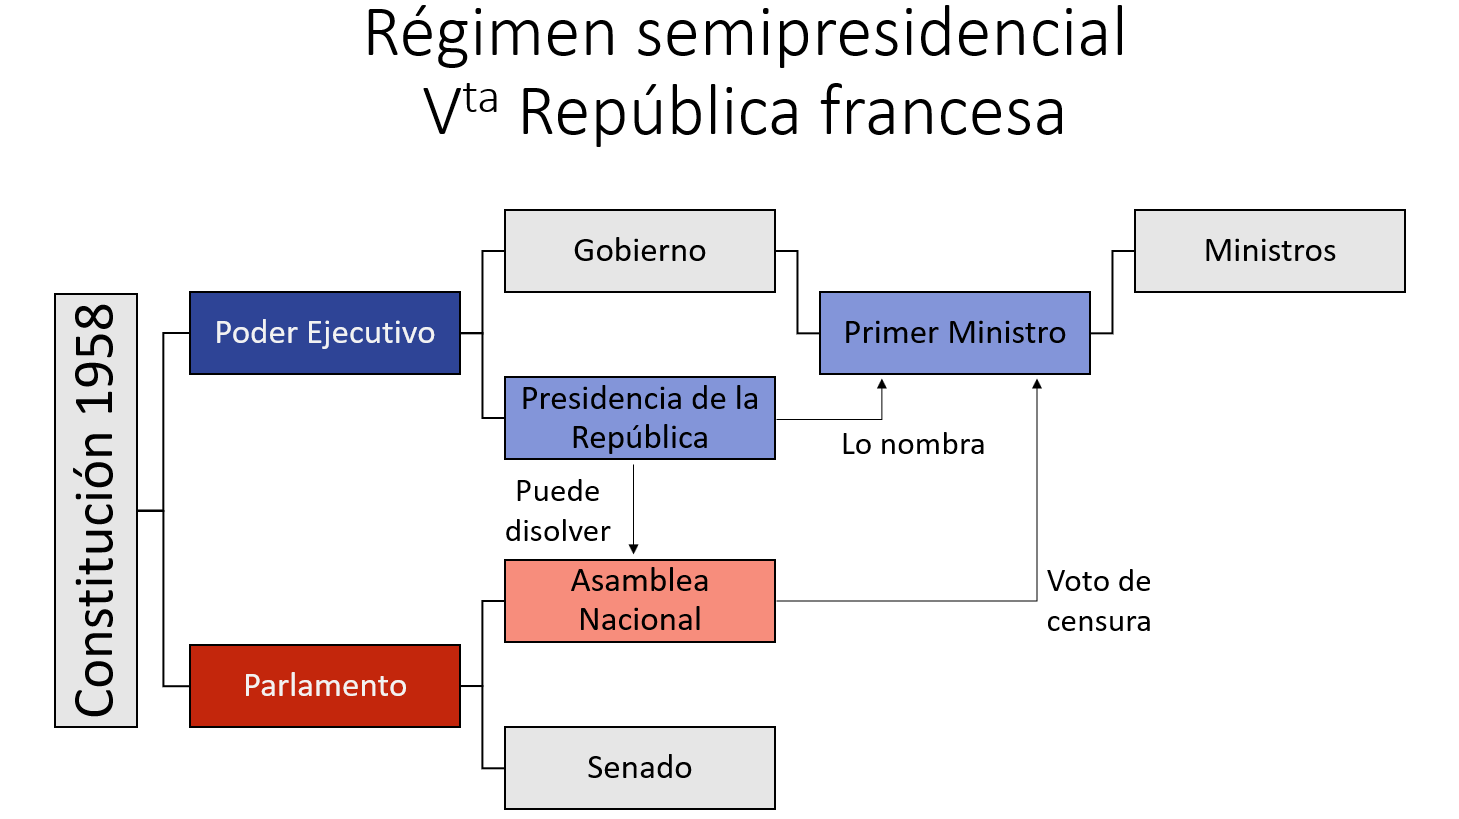
\includegraphics[width = 0.95\textwidth]{Figs/FN_Francia/RegSemiPresFrVta}
	\caption{Esquema del régimen semipresidencial francés de la V\textsuperscript{ta} República. Los poderes ejecutivo--- Presidencia de la República y Gobierno--- y legislativo--- Parlamento bicameral--- están separados. El Presidente nombra al Primer Ministro, quien forma un Gobierno que depende de la confianza de la Asamblea Nacional, misma que puede ser disuelta por el Presidente. Fuente: elaboración propia.}
	\label{fig:Regimen_Semipresidencial_VRepFr}	
\end{figure}


Existen tres mecanismos por los cuales la Asamblea Nacional puede obligar a un Gobierno a renunciar. El primero es usualmente llamado \textit{voto de confianza} y se da cuando el Primer Ministro somete su programa o alguna política general a la confianza de la Asamblea que vota y si la niega, el Gobierno debe renunciar. La segunda es el \textit{voto de censura} que se da por iniciativa de la Asamblea y, en caso de aprobarse, el Gobierno cae. Finalmente el Gobierno, bajo ciertas circunstancias, puede condicionar su responsabilidad a una iniciativa particular: si la Asamblea no está de acuerdo con el proyecto debe censurar al Gobierno y destituirlo o de lo contrario el texto propuesto es aprobado automáticamente \parencite{AN17c}.\\

¿Qué implicaciones tiene esta configuración legal? Como bien apunta \textcite{Carpizo04}, el régimen semipresidencial francés en la práctica es un régimen de alternancias entre un sistema (casi) presidencial y uno (casi) parlamentario. Cuál de estos subsistemas imperará depende de lo que \textcite{Marrani09} llama la sincronía dentro del ejecutivo y que depende de la configuración política de las tres instituciones resaltadas en la \textbf{Figura \ref{fig:Regimen_Semipresidencial_VRepFr}}: la Presidencia, la Asamblea Nacional y, por tanto, el(la) Primer(a) Ministro(a).\footnote{Hasta el momento solo ha habido una Primera Ministra, Édith Cresson (1991-1992).}\\ 

Recordemos que el Presidente es quien nombra al Primer Ministro. Cuando el Presidente logra tener de su lado a la mayoría de la Asamblea Nacional, este puede nombrar a quien quiera sin temor de que la Asamblea vaya a destituirlo. A pesar de que formalmente el Primer Ministro es quien gobierna, en la práctica este le debe deferencia al Presidente y se convierte solo en un facilitador de su política. Esta es la situación donde hay una sincronía al interior del ejecutivo y el sistema es marcadamente presidencial. Se da lo que \citeauthor{Marrani09} llama \textit{fait majoritaire} y que podríamos designar como el funcionamiento bajo mayoría presidencial.\\ 

Sin embargo, cabe la posibilidad de que la Asamblea Nacional tenga una mayoría que se oponga al Jefe de Estado. En este caso, conocido como \textit{cohabitation}, el Presidente ya no puede nombrar a quien quiera. Debe nombrar a alguien que sea apoyado por la mayoría opositora de la Asamblea.\footnote{El Primer Ministro, a diferencia de lo que sucede en un sistema puramente parlamentario, no precisa ser miembro del Parlamento; por el contrario, existe una incompatibilidad constitucional entre la función gubernamental y el mandato parlamentario \parencite{ConstFr}. Ha habido Primeros Ministros que no eran diputados de la Asamblea y, cuando un diputado es nombrado ministro, este debe cesar sus funciones y su suplente lo reemplaza en la Asamblea.} Se da una falta de sincronización al interior del ejecutivo y el Presidente debe cohabitar con un Jefe de Gobierno políticamente opuesto a él. Aquí es cuando estamos en un subsistema de corte parlamentario pues es la mayoría parlamentaria la que gobierna y, salvo en sus dominios de predominancia, los poderes del Presidente se ven fuertemente reducidos.\footnote{Su poder de veto, que no había mencionado, permanece. Sin embargo, el poder de veto en la práctica no es tan relevante como los otros puesto que en situación de mayoría presidencial no es usualmente necesario, mientras que en periodo de cohabitación es más un mecanismo de oposición legislativa que la mayoría de la Asamblea puede superar. El Presidente también conserva su poder de disolución, pero esta es una herramienta riesgosa y costosa políticamente.}\\ 

En la historia de Francia han existido tres cohabitaciones: Miterrand-Chirac (1986-1988), Miterrand-Balladur (1993-1995) y Chirac-Jospin (1997-2002). Han habido también otros periodos en los que formalmente el Primer Ministro no pertenece al mismo partido político que el Presidente pero que sí forma parte de su mayoría presidencial, por lo que no podríamos llamarlos cohabitación. Estos han sido los cuatro gobiernos bajo la presidencia de Giscard d'Estaing--- el primero de Chirac (1974-1976) y los tres de Barre (1976-1977, 1977-1978, 1978-1981)--- así como los dos gobiernos de Philippe bajo la actual presidencia de Macron.\\

Una vez establecido el panorama general del sistema de gobierno en Francia, resulta pertinente hacer referencia a la división territorial del país galo. 

\subsection{División territorial}

De acuerdo con el artículo 72 de la Constitución francesa, 

\begin{quote}
Las colectividades territoriales de la República son las comunas, los departamentos, las regiones, las colectividades con estatus particular y las colectividades de ultramar...
\end{quote}

\begin{figure}[h]
	\centering
	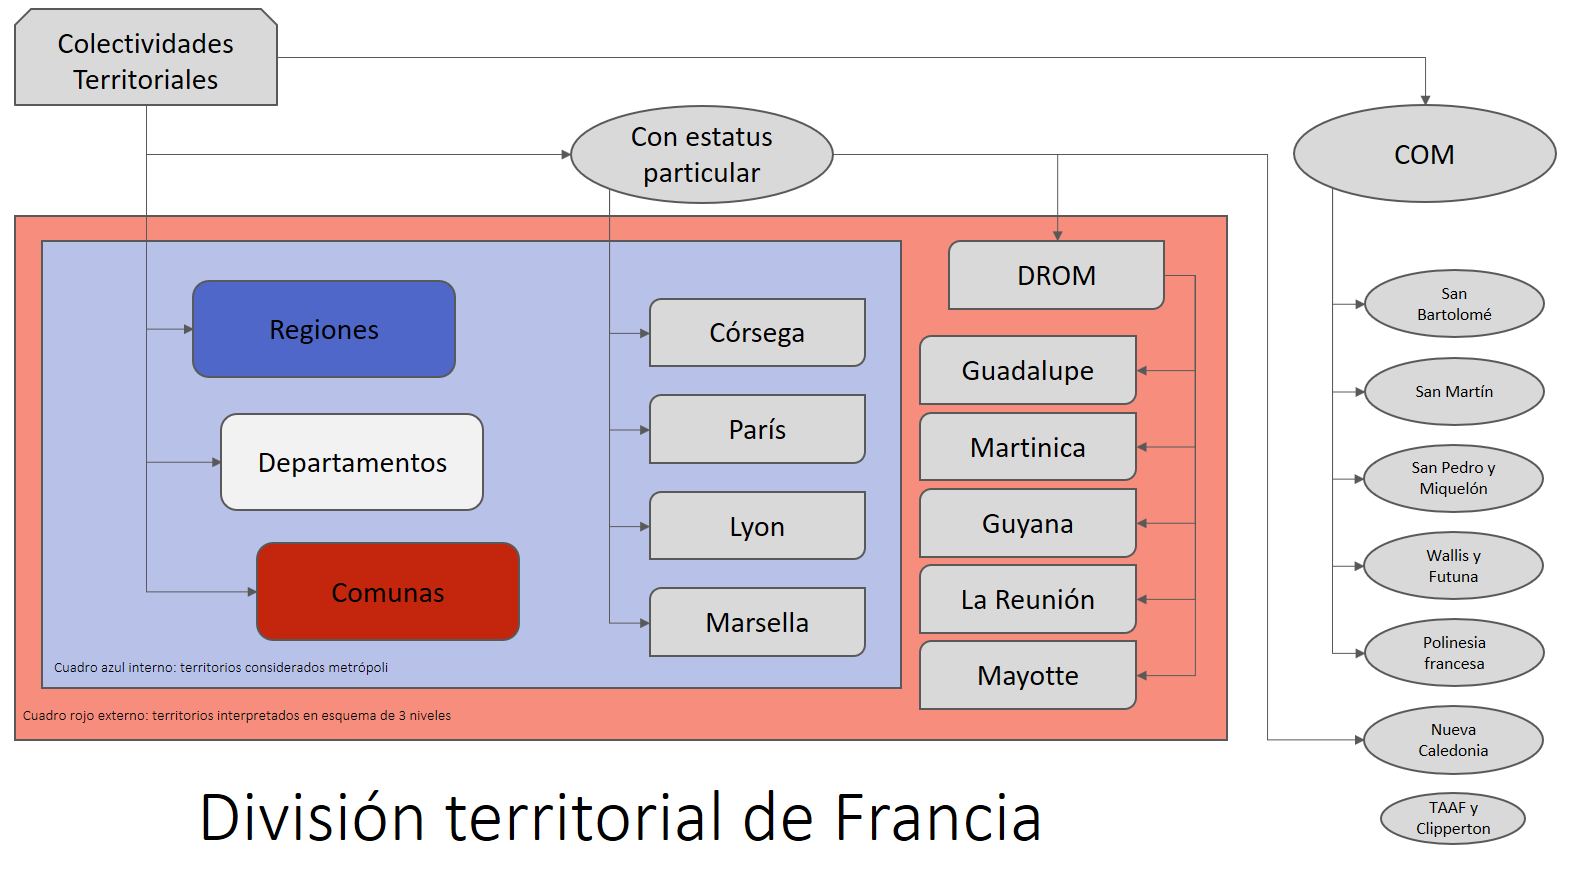
\includegraphics[width = 0.95\textwidth]{Figs/FN_Francia/Div_Terr_Fr_v2}
	\caption{Esquema de la división territorial francesa. Fuente: elaboración propia a partir de \textcite{AN17b}.}
	\label{fig:Div_Terr_Fr}	
\end{figure}

Esta estructura general puede verse en la \textbf{Figura \ref{fig:Div_Terr_Fr}}. Los primeros tres tipos de colectividades territoriales son los más usuales y se refieren a los 3 niveles de administración. El artículo después refiere la existencia de otros dos tipos de colectividades territoriales: las que tienen estatus particular y las de ultramar. No debe pensarse, sin embargo, que estas últimas son todas aquellas que no pertenecen a la metrópoli, identificada en la \textbf{Figura \ref{fig:Div_Terr_Fr}} mediante el recuadro azul interno.\footnote{La metrópoli incluye el territorio continental de Francia--- coloquialmente conocido como el Hexágono, por su forma--- y la isla de Córcega.}\\ 

Más bien se refieren a 5 territorios específicos conocidos en Francia como \textit{Collectivités d'outre-mer} (COM): San Bartolomé, San Martín, San Pedro y Miquelón, Wallis y Futuna, así como la Polinesia francesa. Existen otros territorios del ultramar francés diferentes a las COM. Hay territorios no habitados: la Isla de Clipperton y los Territorios australes y antárticos franceses (TAAF). Encontramos también a la Nueva Caledonia como una colectividad \textit{sui generis}. Finalmente, existen otros 5 territorios de ultramar que son colectividades territoriales con estatus especial, los \textit{Départements et Régions d'outre-mer} (DROM): Guadalupe, Martinica, Guyana, Reunión y Mayotte. Estos 5 DROM y otros 4 territorios en la metrópoli que también son colectividades con estatus especial--- Córcega, París, Lyon y Marsella--- usualmente son considerados dentro del sistema de 3 niveles, a pesar de las particularidades de cada uno. Así pues, el recuadro rojo externo de la \textbf{Figura \ref{fig:Div_Terr_Fr}} identifica a todas las colectividades territoriales que se interpretan bajo el esquema de 3 niveles.\\

Estos tienen las siguientes características generales \parencite{AN17b}: 

\begin{enumerate}
\item \textbf{Comunas} \\ 
Son el nivel más cercano a los ciudadanos. Existen desde 1789 cuando remplazaron a las parroquias. Existen en Francia alrededor de 36,000, aunque año con año el número varía pues las comunas pueden fusionarse o separarse. Sus principales áreas de competencia son el urbanismo, la vivienda y el ambiente. Se gobiernan principalmente mediante un concejo municipal elegido popularmente y un \textit{maire} designado por dicho concejo.

\item \textbf{Departamentos}\\ 
El segundo nivel también fue creado en 1789. Hasta el 31 de diciembre de 2017, existían 101 departamentos, de los cuales 96 formaban la metrópoli y los otros 5 son DROM. A partir del  1ro de enero de 2018 los dos departamentos de Córcega fueron sustituidos por una colectividad única, por lo que ahora hay 100 departamentos. Tienen dos dominios de responsabilidad: la acción social y el manejo de los espacios.\footnote{Estos términos incluyen, el primero, los temas relacionados con grupos vulnerables como la infancia, las personas con discapacidad o los adultos mayores, mientras que el segundo se refiere, por ejemplo, al control de puertos, aeropuertos o caminos dentro del territorio del departamento.} Se gobiernan principalmente mediante un concejo departamental elegido popularmente y un presidente designado por dicho concejo.

\item \textbf{Regiones}\\ 
Es el nivel de más reciente creación, pues fue reconocido como colectividad territorial en 1982. Hasta 2015 existieron 27 regiones, 22 en la metrópoli--- incluída Córcega--- y las 5 DROM. En 2015 hubo una reforma que agrupó algunas, por lo que las nuevas regiones son solo 18--- 13 en la metrópoli, contando Córcega, y las 5 DROM---. Las regiones están encargadas del desarrollo económico, la administración del territorio y los transportes no urbanos. Se gobiernan principalmente mediante un concejo regional elegido popularmente y un presidente designado por dicho concejo.
\end{enumerate} 

Las colectividades territoriales usualmente son de uno de los tres niveles. Por ejemplo, \textit{Villemomble} es una de las 40 comunas que conforman el departamento de \textit{Seine-Saint-Denis}. Este, a su vez, es uno de los 8 departamentos que conforman la región \textit{Île de France}. Sin embargo, las colectividades con estatus especial pueden compartir, al mismo tiempo, dos niveles. Este es el caso de París, que también se encuentra en la región Île de France pero que es tanto un departamento como una comuna dividida en \textit{arrondisements municipales}.\footnote{Nótese que uso la palabra \textit{pueden}; Marsella tiene un estatus especial pero es solamente una comuna.}\\

Una vez que he presentado un resumen general del semipresidencialismo francés y de la organización del territorio, procedo a mencionar a grandes rasgos el sistema electoral del país.

\subsection{Principales elecciones}

Con base en lo que reporta el Ministerio del Interior francés (\citetitle{InterieurElecc}), identifico cuatro categorías de elecciones francesas. 

\begin{itemize}
\item Para conformar los poderes nacionales: 
	\begin{itemize}
	\item Presidenciales. 
	\item Legislativas, para la Asamblea Nacional.
	\item Senatoriales.
	\end{itemize}
	
\item Para conformar las autoridades de los 3 niveles: 
	\begin{itemize}
	\item Municipales, a nivel comuna. 
	\item Departamentales, antes conocidas como cantonales.\footnote{Antes de una reforma de 2015 las elecciones para el nivel de departamento eran conocidas como elecciones cantonales pues los consejeros se eligen en circunscripciones llamadas cantones.}
	\item Regionales.
	\end{itemize}
	
\item Supranacionales:
	\begin{itemize}
	\item Europeas, para el Parlamento europeo.
	\end{itemize}
	
\item Especiales, con diversos fines: 
	\begin{itemize}
	\item Referéndums.
	\item Comunitarias, se dan al interior de las comunas.
	\end{itemize}
\end{itemize}

De entre estas categorías, solo me concentraré en explicar un poco más las presidenciales y las legislativas por tratarse de las dos principales instituciones que determinan el funcionamiento del sistema semipresidencial francés. Ambas son elecciones de sufragio universal directo.\\

La Asamblea Nacional se conforma por 577 diputados que se eligen por periodos de 5 años con reelección.\footnote{A menos que el Presidente disuelva la Asamblea antes del término de la legislatura, en cuyo caso no puede haber una nueva disolución en el año siguiente.} Se elige un diputado por circunscripción legislativa mediante un sistema de mayoría a doble vuelta. Esto significa que hay dos formas de ganar la elección: 

\begin{enumerate}
\item \textbf{En la primera vuelta}, si se obtiene la mayoría absoluta de la votación efectiva, siempre y cuando los votos recibidos representen al menos un cuarto de los electores inscritos en las listas de votación. 
\item \textbf{En la segunda vuelta}, donde basta la mayoría relativa. En caso de empate el(la) candidato(a) de mayor edad gana. 
\end{enumerate}

Pasan a la segunda vuelta todas las candidaturas que hayan obtenido un porcentaje de votación equivalente al menos al 12.5\% de los electores inscritos en las listas de votación. Esto significa que puede haber más de dos contendientes en la segunda vuelta.\footnote{Esto da lugar a las expresiones \textit{duels}, entre dos candidaturas, y \textit{triangulaires}, entre tres. Pueden también darse cuadrangulares o segundas vueltas entre más candidatos pero son mucho menos frecuentes y, cuando suceden, tienden a haber declinaciones y alianzas.}\\

Por otro lado, tenemos la elección presidencial. En el siglo XXI ha habido dos principales reformas consititucionales que han moldeado esta elección. La primera, en 2000, redujo el periodo presidencial de 7 a 5 años. Aunque esto pareciera a primera vista un control sobre el Presidente, en realidad es una reforma que refuerza al Jefe de Estado. Ahora los periodos presidenciales coinciden con los 5 años por los que son elegidos los diputados.\footnote{A menos, claro, que el propio Presidente disuelva la asamblea, cosa que no ha ocurrido desde la reforma. De hecho, solo han existido 5 disoluciones en la V\textsuperscript{ta} República, todas en el siglo XX, en 1962, 1968, 1981, 1988 y 1997.} Más aún, la elección presidencial se realiza unas semanas antes que la elección legislativa. Esto hace mucho menos probable que un presidente electo enfrente una cohabitación, pues su reciente triunfo tiende a impulsar una mayoría legislativa a su favor. Sin embargo, en 2008, se decidió limitar al Jefe del Estado prohibiendo que un presidente sirva más de dos mandatos.\\

Los presidentes también se eligen mediante mayoría a dos vueltas. Esto significa que, al igual que con los diputados, se puede ganar la elección de dos formas: 

\begin{enumerate}
\item \textbf{En la primera vuelta}, si se obtiene la mayoría absoluta de la votación efectiva.  
\item \textbf{En la segunda vuelta}, si se obtiene la mayoría absoluta de la votación efectiva. 
\end{enumerate}

Para garantizar que alguien gane la elección en la segunda vuelta, a diferencia de lo que pasa con las elecciones legislativas, solo pueden presentarse a la segunda vuelta las dos candidaturas más votadas en la primera. Sin embargo, existe un vacío legal en el caso de empate, pues el criterio de edad imperante en las elecciones legislativas no está contemplado para la elección presidencial \parencite{Parisien16}.

\section{Breve historia del Front National}

Como todo fenómeno social, el FN no ha sido un movimiento monolítico. Desde sus orígenes y hasta el día de hoy ha tenido momentos de menor y mayor éxito. Un esquema para estudiar la historia del partido, principalmente desde el punto de vista electoral, considera tres grandes etapas. En primer lugar, la primera década de su existencia estuvo marcada por la marginalidad política y es comúnmente llamada la \textit{traversée du désert}. En segundo lugar, a partir de los años 80 el FN irrumpe en la escena política de la mano de su líder Jean-Marie Le Pen quien, en 2002, logró alcanzar su zenit al obtener el segundo lugar en la primera vuelta presidencial de ese año. No obstante la primera década del siglo XXI estuvo marcada por el declive de la figura de Le Pen. Por ello, en 2011 comienza la más reciente etapa del partido. Jean-Marie Le Pen pasó la batuta del liderazgo a su hija Marine Le Pen quien desde entonces ha implementado una estrategia de \textit{dédiabolisation}, buscando acabar con la imagen negativa del partido, principalmente con respecto al carácter racista que caracterizó a su padre.\\ 

El recuento histórico que sigue está basado primordialmente en aquellos que hacen \textcite{Hainsworth16b} y \textcite{Stockemer17}, así como en el apéndice cronológico al libro editado por \textcite{CreponEtAl15} pero algunas otras referencias se citan también.

\subsection{El FN del desierto (1972-1983)}

El Front National surgió como una iniciativa del movimiento \textit{Ordre Nouveau} (ON) en 1972 para unir en una plataforma electoral a distintos grupúsculos\footnote{En el sentido de grupos más bien pequeños y dispersos.} políticos extremistas como los irredentistas de la colonización francesa en Algeria, los herederos del movimiento poujadista o del régimen de Vichy, intelectuales de la \textit{Nouvelle Droite}, organizaciones juveniles como \textit{Occident} o \textit{L'\OE{}uvre Française}, revisionistas del Holocausto, monarquistas, entre otros. Jean-Marie Le Pen fue elegido presidente del partido, en parte por ser una figura relativamente conocida--- se había convertido en el diputado más joven en 1956 como parte del movimiento de Poujade y había sido el coordinador de campaña de Tixier-Vignancour en 1965--- y en parte por, irónicamente, ser visto como un moderado.\\ 

Durante los años siguientes, sin embargo, el nuevo partido hiló una serie de fracasos electorales en las elecciones legislativas de 1973, las presidenciales de 1974, las legislativas de 1978 y, de manera más particular, en las presidenciales de 1981, en las cuales Le Pen no logró las firmas necesarias para participar.\footnote{En Francia, para que una persona se pueda presentar como candidata en las elecciones presidenciales requiere 500 apadrinamientos de parte de representantes electos como pueden ser alcaldes o legisladores.} Los problemas no se limitaron a las urnas. Ya desde 1973 la multiplicidad de facciones hizo que el partido se debilitara. Después de un mitin llamado \textit{Alto a la inmigración salvaje} miembros de ON se enfrentaron en una batalla campal violenta con miembros de la Liga Comunista por lo que el movimiento fue proscrito. Esto le permitió a Le Pen tomar mayor control del partido, pero también hizo surgir en 1974 a un nuevo partido fundado por miembros de ON, el PFN (\textit{Parti des Forces Nouvelles}). En 1976 Le Pen sobrevivió a un intento de asesinato pero su segundo al mando e ideólogo, François Duprat, fue asesinado por un coche bomba en 1978. El Front National parecía apenas sobrevivir.\\

Entonces, el partido comienza a poner en un segundo plano su carácter anticomunista para hacer mayor énfasis en la migración vinculando a los inmigrantes con los problemas de seguridad y desempleo. A inicios de los años 80, sus posturas nativistas, autoritarias y populistas empezaron a resonar en los votantes. La presidencia de Miterrand implementó varias medidas para facilitar la inmigración, reducir las prerrogativas de la policía y otorgó amnistías a casi el 14\% de los prisioneros. La población francesa no fue del todo favorable a ello. Los partidos tradicionales de derecha comenzaron a endurecer sus posturas frente a la migración y la seguridad. Esto le dio mayor legitimidad al FN pues le permitió normalizar, de cierta manera, su discurso.\\ 

A nivel local, el FN comienza a crecer en Dreux donde en las elecciones legislativas de 1981 logró obtener más de 10\% de los votos. En las elecciones municipales de 1983 de París Le Pen es nombrado consejero municipal del distrito 20 al obtener 11.26\% de los votos en la primera vuelta y 8.54\% en la segunda. Jean-Pierre Stirbois en Dreux logra incluso un mejor resultado: 16.72\% de los votos en la primera vuelta y una alianza con la derecha tradicional en la segunda vuelta lo llevan también a ser consejero municipal. El partido había atravesado un desierto político y estaba a punto de sorprender a propios y extraños.

\subsection{El FN Lepenista (1984-2010)}

La hora de la verdad de Le Pen, literalmente, llegó en 1984. El éxito en Dreux hizo que Le Pen fuera invitado en febrero de ese año al programa político de TV más visto en Francia entonces, \textit{L'heure de verité}. La entrevista fue todo un éxito; las preferencias electorales del FN pasaron del 3.5\% al 7\% a la semana siguiente de la entrevista, por ejemplo \parencite{Stockemer17}. Simbólicamente podría marcar el inicio de lo que aquí llamo la era lepenista del FN, cuya confirmación fue el 17 de junio de 1984. Las listas del FN lograron aproximadamente 11\% de los votos en las elecciones al Parlamento Europeo que se transformaron, gracias al sistema proporcional, en 10 eurodiputados de extracción frontista. El FN ya no era un partido al margen del sistema político, lo que le permitió captar más liderazgos.\\ 

El más importante de esos nuevos adherentes fue, sin duda, Bruno Mégret. En 1985 se unió al partido y en 1988 se conviertió en director general. La adición de Mégret demostraría ser fundamental para la consolidación del FN como un actor político relevante en Francia. A él se le atribuye la profesionalización de los cuadros y estructuras del partido así como la popularización de la retórica frontista y, en gran medida, el que en las elecciones de la segunda mitad de los 80 el FN haya obtenido alrededor del 10\% de manera consistente: 9\% en las cantonales de 1985, 10\% en las legislativas de 1986, 14\% en las presidenciales de 1988, 9\% en las legislativas de 1988, 11\% en las europeas de 1989, así como el primer alcalde frontista en 1989.\\ 

En los años 90 el FN continuó creciendo en las preferencias electorales, de la mano del populismo de Le Pen y la organización de Mégret. En 1995, los candidatos del FN se convirtieron en alcaldes en tres ciudades relevantes: Toulon, Marignane y Orange. En las elecciones presidenciales de 1995, las legislativas de 1997 y las regionales de 1998 el frontismo se afianzó alrededor del 15\% de los votos.\\

Empero, los éxitos no estuvieron alejados de los escándalos. A pesar de los intentos de Mégret por encuadrar el nativismo del FN en conceptos políticamente más correctos--- que no más moderados--- como la \textit{preferencia nacional}, el antisemitismo de Le Pen y de otros miembros del FN era evidente. En varias ocasiones Le Pen fue centro de atención por sus comentarios. Los más conocidos son quizás cuando dijo que el Holocausto era un ``pequeño detalle'' en la historia de la Segunda Guerra Mundial o cuando se burló de un ministro de nombre Michel Durafour llamándolo \textit{Monsieur Durafour Crématoire}.\footnote{La palabra \textit{four} en francés significa horno y agregó el término \textit{crématoire}, es decir, crematorio.}\\ 

Asimismo, con los éxitos también surgieron las rivalidades internas. El liderazgo de Mégret empezó a ser más evidente e incómodo para Le Pen. Ambos personajes tenían también visiones distintas sobre la estrategia del partido;  mientras Mégret abogaba por tejer alianzas con los partidos de la derecha tradicional, Le Pen siempre las rechazó, lo que a los seguidores de Mégret les hacía creer que en realidad no quería llegar al poder. Las tensiones fueron creciendo hasta llegar a un enfrentamiento directo entre 1998 y 1999.\\ 

En 1997, Le Pen había ido a Mantes-la-Jolie a apoyar a su hija en su campaña en las legislativas de ese año. Al llegar al lugar fue recibido por manifestantes que lo increparon, llamándolo fascista. Desde que bajaron del carro, los guardaespaldas de Le Pen comenzaron a golpear a los manifestantes y eso desató una pelea en la que el propio Le Pen se involucró. En un momento empujó contra un muro a la rival de su hija, la socialista Annette Peulvast-Bergeal \parencite{InaPolitique97}. Por este ataque, Le Pen fue condenado en 1998 a un año de inegilibilidad, a tres meses de prisión suspendida condicionalmente y a 5,000 francos de multa \parencite{LesEchos99}. Así pues, Le Pen estaba impedido para participar en las elecciones europeas de 1999. Mégret parecía la opción más natural para encabezar las listas del partido. Sin embargo, parafraseando a Le Pen, en el FN el único que importaba era el número uno, así que colocó a su esposa en el primer puesto en lugar de a Mégret.\\ 

En diciembre de 1998, Mégret criticó a Le Pen y dijo que se había convertido en un lastre para el partido. El comité ejecutivo del partido, controlado por Le Pen, votó para expulsar a Mégret del FN. En respuesta, Mégret fundó un nuevo partido, el MNR (\textit{Mouvement National Républicain}). El cisma mégretista se llevó a casi la mitad de los miembros del FN y a su más importante operador político. Compitiendo contra el MNR, en las elecciones europeas de 1999 el frontismo solo obtuvo el 5.7\% de los votos.\\ 

No obstante, el más grande éxito de Jean-Marie Le Pen llegó apenas unos años después. Ante una izquierda sumamente dividida--- hubo 8 candidatos de izquierda--- en una elección presidencial atípica, Le Pen sacudió a propios y extraños el 21 de abril de 2002. En total 16 candidaturas lograron las firmas necesarias para competir, un récord en Francia. Nadie logró más de 20\% de los votos en la primera ronda, algo también inédito. Los estrategas de los candidatos no creían lo que sus conteos rápidos les decían. A las 8 de la noche, las cadenas de televisión dieron la noticia: Jean-Marie Le Pen había quedado en segundo lugar, apenas por encima del candidato socialista, Lionel Jospin. La diferencia había sido de menos de 200 mil votos.\\ 

En Youtube se puede encontrar un documental en francés que refleja de muy buena manera cómo se vivió esa noche electoral en Francia \parencite{Capo17}. Del lado socialista, incredulidad, sorpresa absoluta y llanto de tristeza. Del lado del FN, también hubo incredulidad, sorpresa absoluta y llanto, pero de emoción. Le Pen había avanzado a la segunda vuelta presidencial. Se enfrentaría al ganador de la primera, el presidente en funciones, Jacques Chirac. Hubo fuertes llamados a unirse en torno a Chirac para evitar que ganara el candidato FN. Ante la amenaza que--- para la enorme mayoría de los franceses--- representaba Le Pen, Chirac fue reelecto por un amplísimo margen: 82\% vs 18\%.\\

Así pues, 2002 fue el gran éxito de Jean-Marie Le Pen, pero también el inicio del fin: era claro que la mayor parte de la población no veía en él una opción aceptable. Los resultados electorales que siguieron fueron en declive: 10\% en las europeas de 2004, 11\% en las presidenciales de 2007, 4\% en las legislativas de 2007, 6\% en las europeas de 2009. Fiel a su costumbre, Le Pen siguió mostrando su revisionismo de la Segunda Guerra Mundial al declarar en 2005 que: ``al menos en Francia, la Ocupación alemana no fue particularmente inhumana''. El partido enfrentó problemas económicos y deudas que lo obligaron a despedir a un tercio de los empleados, a cancelar su fiesta \textit{Bleu Blanc Rouge}, entre otras cosas. Era claro que Jean-Marie Le Pen ya no estaba en condiciones de liderar al Front National. Sin embargo, el líder histórico no habría de ceder el mando a cualquiera.

\subsection{El FN Marinista (2011-2018)} 
 
Cuando fue momento de pasar la batuta de su movimiento, y a pesar de que existía mucho apoyo al interior del partido para que Bruno Gollnisch--- un viejo lobo de mar del FN--- fuera el nuevo líder, Jean-Marie Le Pen decidió apoyar a su hija, Marine Le Pen. En una elección interna anterior para el liderazgo del comité central del partido, Gollnisch había ganado mientras que Marine Le Pen había quedado en una lejana posición número 34 \parencite{Williams12}. A pesar de ello, el 16 de enero de 2011, Marine Le Pen fue elegida presidenta del FN, mientras que Jean-Marie Le Pen fue nombrado presidente honorario del mismo.\\ 

La estrategia del \textit{marinisme}, en contraposición a la del \textit{lepenisme}, ha buscado \textit{desatanizar} al partido. Marine Le Pen ha querido renovar la imagen que el FN presenta a los electores. Si el FN lepenista siempre fue muy vocal respecto a sus posiciones sobre los temas de prácticas y costumbres sociales o, como se les conoce en Francia, las \textit{m\oe{}urs}, bajo el liderazgo marinista, la posición oficial del FN al respecto ha cambiado. El símbolo de esta inflexión en temas sociales quizás es Florian Philippot--- vicepresidente del partido de 2012 a 2017--- quien en 2014 declaró ser gay, algo impensable en el FN lepenista.\footnote{Digo inflexión porque no ha sido un cambio total: hay cuadros que mantienen posiciones firmes en contra del aborto o los matrimonios entre personas del mismo sexo, sin embargo, la postura oficial ha sido más ambigua y ha dejado de hacer énfasis en esos temas. El lector interesado en el tema de las m\oe{}urs dentro del FN puede consultar el texto de \textcite{Crepon15}.}\\ 

Por otro lado, y de manera muy particular, Marine Le Pen ha cortado al interior del partido las expresiones antisemitas y abiertamente racistas. A diferencia de lo que dijo su padre, ella ha declarado que todo el mundo sabe lo que pasó en los campos nazis, en qué condiciones sucedió y cómo representó la máxima expresión de la barbarie. De hecho, a raíz de que Jean-Marie Le Pen reafirmara en 2015 el caracter de ``pequeño detalle'' del Holocausto, Marine Le Pen empujó y consiguió la expulsión de su padre del partido.\\

Esta estrategia parece haber rendido sus frutos con el electorado. A pesar de no avanzar a la segunda vuelta en 2012, Marine Le Pen superó a su padre al obtener 18\% de los votos en la primera vuelta. En las legislativas de ese año, el FN obtuvo dos diputaciones y el 14\% de los sufragios. En 2014, el partido conquistó 11 alcaldías, sus primeros dos senadores y fue la primera fuerza política votada en las elecciones europeas con 25\%. Este crecimiento ha continuado, pues en 2015 el FN obtuvo el 25\% en las elecciones departamentales y el 28\% en las regionales.\\ 

En las elecciones presidenciales de 2017, la lideresa del frontismo logró superar de nueva cuenta a su padre. Ella obtuvo 21\% de los votos de la primera vuelta, más que Jean-Marie Le Pen en 2002, lo que le permitió también avanzar a la segunda vuelta. Sin embargo en 2017, a diferencia del 2002, la presencia del FN en la segunda vuelta no fue sorpresiva sino más bien era lo esperado. Más aún, si Le Pen padre perdió dicha segunda vuelta por una diferencia de alrededor de 65 puntos porcentuales, Le Pen hija la perdió por poco más de 30. Los franceses volvieron a dejar claro que consideran, mayoritariamente, al FN como una amenaza; empero, esa percepción ha disminuido fuertemente en la era marinista del partido.\\

A pesar de estos éxitos de la estrategia de desatanización, existen varios paralelismos con la historia de su padre. Así como Jean-Marie Le Pen tuvo a Bruno Mégret como su operador político, Marine Le Pen se apoyó en Florian Philippot para encuadrar su discurso y manejar al partido. Ambas manos derechas de los Le Pen, terminaron por salir del partido y fundar su alternativa política, aunque los motivos y circunstancias de los cismas fueron distintos. Como ya he dicho, Mégret fue expulsado después de desafiar directamente a Jean-Marie Le Pen por el liderazgo del partido. La renuncia de Philippot al FN, por el contrario, surge en medio de una introspección del partido y la búsqueda de culpables después de las elecciones de 2017.\\ 

Las elecciones presidenciales de 2017 marcaron la mayor cantidad de votos en la historia del FN. 33\% en la segunda vuelta no es un dato menor, sin embargo, para muchos significó un fracaso. Bruno Jeudy, Vanessa Schneider, Nonna Mayer y Jérôme Fourquet discutieron al respecto en el programa de televisión \textit{\textcite{CDansLAir17}}: muchas encuestas a lo largo del proceso apuntaban a que Le Pen lograría hasta 40\% de los sufragios hasta que la noche del debate entre Le Pen y Emmanuel Macron se dio un punto de inflexión. Marine Le Pen fue muy agresiva--- minando, posiblemente, el esfuerzo de desatanización--- pero también se vio poco preparada. En un momento Macron le preguntó si ella proponía abandonar el euro y regresar al franco como moneda francesa. Su respuesta fue ambigua y muy poco clara. El debate supuso un duro golpe que le habría hecho perder al menos 5 puntos porcentuales de intención de voto.\\

La postura de abandonar el euro no fue la más popular entre el electorado e incluso dentro de buena parte de los miembros del FN. Esta propuesta, como la mayoría del programa económico del FN, se debe a Philippot y su corriente que podríamos llamar soberanista en contraposición a la línea identitaria más dura del partido \parencites{Marin17}{Berteloot17}{Europe17}. Mientras que Philippot buscaba poner más énfasis en los temas económicos y sociales, que pudieran atraer a más electores--- particularmente de izquierda, los llamados \textit{gaucho-lepenistes}--- otros cuadros del partido buscarían resaltar la línea de inmigración y seguridad de corte más derechista.\\ 

Philippot fue señalado como el culpable de la decepción. Formó una organización política interna al FN llamada \textit{Les Patriotes} y amenazó con abandonar el partido si el FN renunciaba a su posición sobre el euro. Después de las elecciones legislativas, en las que el FN logró 8 escaños pero no los 15 necesarios para convertirse en grupo parlamentario, las presiones aumentaron. Marine Le Pen le pidió elegir entre la vicepresidencia del FN y la dirección de \textit{Les Patriotes} y él respondió acusando al partido de estar cambiando de línea y regresando a un pasado absolutamente horripilante. Su destino estaba sellado: le fueron retiradas sus responsabilidades como vicepresidente y Philippot renunció al FN para convertir a \textit{Les Patriotes} en un nuevo partido político \parencites{Galtier17}{Zafimehy17}.\\

A raíz del resultado electoral de 2017, Marine Le Pen impulsó la idea de una refundación del partido. El electorado francés había vuelto a dejar claro que la marca FN estaba vetada del Elíseo. Por ello, propuso un cambio de nombre. A partir de 2018, el \textit{Front National} se convirtió oficialmente en \textit{Rassemblement National}. Así pues, la era marinista del FN terminó en 2018.\\ 

En la primera elección del RN, las europeas de 2019, Marine Le Pen decidió no ser candidata. Esto no necesariamente quiere decir un abandono de la centralidad de Le Pen. De hecho, el nombre oficial de la lista fue \textit{Prenez le pouvoir, liste soutenue par Marine Le Pen}--- Tomar el poder, lista apoyada por Marine Le Pen---. Sin embargo, la estrategia fue continuar con la imagen del cambio de marca del partido, particularmente en términos generacionales. La lista fue encabezada por el joven portavoz del partido, Jordan Bardella, de apenas 23 años. Con Bardella a la cabeza, RN obtuvo un cerrado primer lugar con 23.34\% de los votos efectivos contra 22.42\% de la lista del movimiento del presidente Macron, la República en Marcha.\\ 

Qué le depara al \textit{pater familia} de los movimientos NAP es incierto. Los partidos políticos tradicionales de Francia han perdido su posición central. Pero con Trump en EUA o Salvini en Italia, Le Pen ya no es siquiera la cara mundial del nativismo autoritario de corte populista. No obstante, sigue siendo uno de los partidos importantes de esta corriente y estudiarlo es un buen punto de partida para aproximarse al fenómeno general de esta familia política. 



	\chapter{Teorías sobre el voto NAP}

En esta tesis, estoy interesado en explorar las \textit{configuraciones sociales} donde se desarrolla o no el voto por un partido NAP específico. Si uno hace una revisión hemerográfica o en internet sobre los motivos de éxito de Trump o el Brexit encontramos que predominan fuertemente las explicaciones de carácter económico y/o cultural \parencites{Beauchamp16a}{Beauchamp16b}{Carney16}{Tesler16}{Sides16} {Arnade16}.\\ 

¿Son los desplazados por la globalización los que votan por los NAP? Los trabajadores del Rust Belt le habrían costado la presidencia a Hillary Clinton, la escolaridad es un clivaje frecuentemente mencionado, existiría un voto de izquierda económica detrás de estos movimientos... ¿O es en realidad una reacción cultural frente a la presencia de aquellos que se consideran como el \textit{Otro}: musulmanes, latinos, negros, inmigrantes en general? Estos fenómenos se están dando en sociedades con población predominantemente blanca y dentro de la cultura occidental, lo que podría interpretarse como un choque de culturas. Así pues, desde el estudio académico, el debate parece estar entre dos \textit{resentimientos} distintos, el económico y el racial/cultural, sin que haya \textit{a priori} uno incontroversialmente dominante sino que más bien están relacionados entre sí \parencites{Inglehart16}{Ivarsflaten14}.\\ 

Para realizar un análisis de este tipo hay que recordar que dentro de la metodología de política comparada existen cuatro grandes paradigmas: institucional, instrumental, cultural y estructural \parencite{Uribe16}. Tomando en cuenta estas primeras ideas y la naturaleza del estudio de caso, me parece que un buen punto de partida es considerar los enfoques estructural y cultural, más que las perspectivas institucional o instrumental.\\  

\section{Estructuralismo y Culturalismo} 

Desde el paradigma estructural, se dice que ``las estructuras condicionan el resultado'' \parencite{BV08}. El concepto tradicional de estructura se refiere a grupos con características materiales distintas. Por ejemplo, el estructuralista socioeconómico por antonomasia resulta Marx. Para él, las profundas fuerzas sociales seguirían un proceso histórico lineal que pasaría del feudalismo al capitalismo y después al socialismo, para culminar en el comunismo \parencite{BV08}. Los cambios tecnológicos impulsarían un sistema económico con nuevas clases sociales que desplazarían las viejas instituciones, refiere \textcite{Heilbroner92} al hablar de la teoría marxista. Con la revolución industrial habrían llegado dos clases sociales encontradas: la burguesía y el proletariado. La Historia marxista sería inevitable, dice el Manifiesto Comunista \parencite{Heilbroner92}: 

\begin{quote}
[El desarrollo de la industria moderna] derriba los fundamentos mismos por los que la burguesía produce y apropia la producción. Lo que la burguesía produce entonces son, sobre todo, sus propios sepultureros. Su caída y la victoria del proletariado son igualmente inevitables...
\end{quote}

Hasta ahora no hemos verificado empíricamente esas afirmaciones de Marx y Engels, pero varias de sus herramientas teóricas siguen vigentes. Lo que la lucha de clases entre el proletariado y la burguesía ejemplifica es que, dentro de las sociedades, existen grupos cuyos intereses están enfrentados. La pertenencia a una de estas clases determinaría, primordialmente, las preferencias políticas de un individuo.\\

Por otro lado, el enfoque cultural tiene como unidad de análisis las ideas y valores existentes en una sociedad. 
De acuerdo con Sheri \textcite{Berman01}, una de las preguntas teóricas que este paradigma busca responder es cómo las variables culturales e ideológicas influyen en el comportamiento político de los individuos. Un ejemplo de esto es el libro \citetitle{AlmondVerba63} \parencite{AlmondVerba63}--- generalmente considerado como el precursor de esta corriente--- que propone cómo diferentes culturas políticas llevarían a distintos grados de estabilidad democrática. Otro ejemplo son los análisis que asocian las preferencias partidarias con ciertos valores e ideas, como el que realiza Ronald Inglehart en 1977 con su teoría de la revolución silenciosa. Para Inglehart, las condiciones económicas de la posguerra con la que crecieron los jóvenes europeos--- mejores con relación a las de sus padres--- habrían hecho que se formaran en valores postmateriales como el sentido de pertenencia y la realización personal \parencite{Kesselman79}. Esto, a su vez, se relacionaría con preferencias por partidos que él llama libertarios de izquierda \parencite{Inglehart16}.\\ 

Considero, siguiendo en parte a \textcite{Sewell92}, que estos dos paradigmas pueden coexistir. Las estructuras pueden ser culturales, así como cambios en las condiciones materiales pueden llevar a cambios ideológicos. En el argumento de Inglehart esto es claro, pero la implicación va más allá. Los desarrollos económicos, así como los cambios en las relaciones de poder o la entrada de nuevos grupos sociales puede forzar un replanteamiento de las creencias existentes \parencite{Berman01}. Cuando hablo de estructuras, entonces, me refiero en un sentido informal a las condiciones ideológicas o materiales que moldean diferentes grupos sociales con intereses distintos. Así pues, en lo subsecuente es bajo esta idea general de estructuras que planteo las posibles explicaciones del voto NAP.\\ 

\section{Clivajes y Escolaridad}

Un constructo teórico útil es el de clivaje político. El principal foco de la teoría de clivajes es la ``evolución a largo plazo de la estructura social'', en donde yacen las ``fuerzas más fundamentales de la política'' \parencite{Bornschier09}. Rokkan y Lipset son las referencias obligadas con respecto a los clivajes tradicionales, pero Bartolini presenta una conceptualización más clara. Un clivaje es una división política que cuenta con tres elementos: división socioestructural, identidad colectiva y manifestación organizacional \parencite{Bornschier09}.\\

Es decir, para que una división en la sociedad pueda considerarse como un clivaje, debe existir una diferencia clara en términos socioestructurales, y que los miembros de cada grupo que constituya dicha distinción formen una identidad colectiva y cierta capacidad de movilización. Estas tres características, la teoría indica, llevarían a que los miembros de cada grupo del clivaje voten de acuerdo a los intereses del mismo. La pertenencia a uno de los lados de la estructura determinaría las preferencias políticas del individuo, traducidas en su voto.\\

Con relación a los movimientos NAP, un clivaje determinante resultaría ser el de ciudadanos escolarizados frente a los no escolarizados.\footnote{Muchos hablan de ciudadanos educados y no educados, pero considero que el término correcto debe ser escolarizados o academizados pues la diferencia socioestructural es la asistencia a una institución académica de nivel medio superior o superior, cosa que no garantiza \textit{per se} la \textit{educación} del individuo, máxime que este es un concepto sujeto a debate, súmamente subjetivo, esquivo y cargado.} Por ejemplo, la primera realización de la segunda vuelta presidencial en Austria en 2016 arrojó en las encuestas una clara división entre aquellos con nivel escolar obligatorio y aquellos con niveles de escolaridad media superior y superior \parencite{Hoare16}. En Estados Unidos, de acuerdo con Nate \textcite{Silver16}, la escolaridad fue el clivaje que mejor predijo quién votaba por Donald Trump. \textcite{Rae16} encontró también una fuerte relación entre el porcentaje de voto antieuropeo en el referéndum británico de 2016 y el porcentaje a nivel local de personas poco escolarizadas.\\ 

Este clivaje, de acuerdo con Hervé \textcite{LeBras15}, tiene consecuencias socioeconómicas directas al tiempo que contribuye a la formación de una clase--- al menos en Francia--- temerosa frente a su posición en la estructura social y susceptible de votar por el Front National. Desde los 90, se ha identificado a los individuos con escolaridad técnica o no universitaria, como un nicho electoral para el FN \parencites{MayerPerrineau90}{Perrineau99}{Gombin05}{Mayer05}{Mayer07}{Perrineau07}{Riviere12}{Perrineau12}. 

\section{La Clase Desplazada por la Globalización}

Por otro lado, en la discusión actual sobre los movimientos NAP, no es raro encontrar referencias al fascismo. Por ejemplo, el número de octubre de 2016 de la revista Letras Libres, dedicado a Donald Trump, presentó una sugerente portada con la foto del magnate y un bigote al estilo Hitler formado por las palabras \textit{Fascista Americano} \parencite{Fascista16}. Otro ejemplo es el carácter neofascista de Norbert Hofer, ver \textcite{Hoare16}. En este sentido resulta pertinente recordar el estudio que desarrolló Barrington Moore respecto del fascismo del siglo XX.\\ 

Desde una perspectiva estructural, Moore explica el surgimiento del fascismo en Alemania, Italia y Japón. La modernización conservadora y la industrialización, frutos de una \textit{revolución desde arriba}, llevaron a contradicciones estructurales fuertes en estos países. El fascismo fue un intento de hacer \textit{popular y plebeyo} el conservadurismo y el reaccionismo, que habían perdido su legitimidad, dice \textcite{Moore66}. La característica principal del fascismo del siglo XX es el anticapitalismo plebeyo. En términos de voto, por ejemplo, los Nazis fueron más populares entre aquellos que tenían menos y estaban más desfavorecidos \textit{con relación al área particular en la que vivían} \parencite{Moore66}.\\ 

\textcite{Sides16} presentan cierta evidencia de que este fue el caso en Estados Unidos con el apoyo hacia Donald Trump, \textcite{Arnade16} habla de la concentración de la prosperidad en el Reino Unido como posible catalizador del voto para el Brexit y \textcite{LeBras15} examina el mapa del voto frontista en Francia frente a un índice de desigualdad socioeconómica en el mismo espíritu con el que Moore refiere el voto Nazi en el espacio rural alemán de inicios de los años treinta pero de una manera mucho más detallada.\\

Ciertamente Moore no es el único teórico que señala el vínculo entre una fuerte modernización económica y el voto hacia los movimientos extremos por parte de clases desfavorecidas: 
\begin{quote}
Al evaluar su propia situación las personas hacen comparaciones con la situación de los demás. Los votantes con una situación socioeconómica débil pueden evaluar esta posición de forma más negativa en tanto vivan en una región acaudalada. Entonces, desigualdades en el ingreso pueden traducirse en apoyo a partidos de derecha extrema \parencite[traducción propia]{Coffe07}.
\end{quote} Esta línea de investigación argumentaría por qué estamos viviendo hoy estos movimientos NAP.\\ 

Para Branko \textcite{Milanovic16}, la globalización iniciada a finales del siglo XX--- y vigente en nuestro siglo--- constituye el más grande cambio en la distribución de los ingresos desde la revolución industrial. Esta redistribución ha traído crecimiento económico, pero de manera muy variada a lo largo de los percentiles poblacionales. Así como el 5\% más rico ha seguido creciendo por encima del promedio, los primeros 70 percentiles lo han hecho a diferentes tasas. Sin embargo, el crecimiento que llama más la atención es el de la población entre el percentil 70 y 95: han crecido menos que la media o incluso han visto su ingreso real disminuir. ¿Quiénes son estas personas? Siete de cada 10 provienen de los \textit{viejos países ricos} de la OCDE.\footnote{Esta evidencia ha llegado a ser conocida como la gráfica del elefante debido a su forma. Ver \textcite{Milanovic16}.} Precisamente muchos de los países en los cuales vemos estos movimientos NAP prosperar. Claro que deducir que esto es prueba de que son estas personas quienes votan por los movimientos NAP sería un error, pues se caería en un caso de falacia ecológica.\\

En el caso particular del FN, no obstante, hay varios estudios que sugieren que han sido las personas de la \textit{clase media} las que han tendido a apoyar al partido. El modelo sociológico de \textcite{MayerPerrineau90} refiere la existencia de una diferencia por nivel de sueldo y posesión de patrimonio. La pequeña burguesía ha sido históricamente asociada a movimientos de derecha \parencites{Mayer87}{LeBras15}{Goodliffe19}. Adicionalmente, en Francia la literatura consistentemente analiza el fenómeno electoral desde la perspectiva de las \textit{categorías socioprofesionales} a las que pertenecen los individuos. Por ejemplo, la mayor o menor presencia de obreros o agricultores, han influido de distinta manera en el comportamiento de los pequeños empresarios en Francia \parencite{MayerMichelat81}. Una lista de referencias que utilizan la variable de categorías socioprofesionales para estudiar al FN son \textcites{Mayer87}{Mayer05}{Mayer07}{MayerPerrineau90}{MayerBoy97}{Perrineau99}{Perrineau07}{Perrineau12}{Gombin05}{Gombin09}{Gombin13}{Gombin13b}{Riviere12}{GombinRiviere13}. En este sentido, esta tendría que ser una de las variables obligadas en mi análisis.

\section{Teorías del Conflicto}

Otros modelos que pudieran encajar con este comportamiento de crecimiento en las preferencias por movimientos NAP son la \textit{teoría del conflicto} y la \textit{teoría del interés económico}. La primera constituye una explicación consistente con ciertos argumentos culturales sobre la motivación racista. Esta teoría es expuesta por autores como \textcite{Blalock67,Olzak92}--- citados por \textcite{Coffe07}---. La violencia étnica, expresada en manifestaciones xenófobas propias de los movimientos NAP, proviene del resentimiento. La clase privilegiada de la sociedad--- pensemos aquí en el tradicional grupo de hombres blancos que mencionan los culturalistas--- comienza a acumular un ``sentimiento de injusticia cuando ve su privilegio escurrirse hacia las manos de otro grupo que no lo tenía antes'', por lo que una ``causa de la violencia étnica es el cambio en estatus legal y político de los grupos étnicos mayoritarios y minoritarios''--- \textcite{Petersen02} citado por \textcite{Beauchamp16b}, traducción propia---.\\ 

 \textcite{Blalock67} y \textcite{Olzak92} teorizan sobre que el conflicto aumenta en zonas de problemas económicos, como el desempleo, y ahí se suceden reacciones exclusionistas por parte de los grupos mayoritarios. Si al resentimiento sumáramos el miedo por competir por la escasez de los recursos, podría sugerirse el por qué los trabajadores manuales con menores niveles escolares tenderían a reaccionar frente a los grupos de inmigrantes. Esta es la lógica de la teoría del interés económico: la presencia de inmigrantes resulta en un aumento en la competencia por recursos escasos y, por lo tanto, en conflictos entre grupos sociales \parencite{Coffe07}.\\ 

Estas teorías son consistentes con el concepto de chauvinismo del bienestar: la propuesta de que los beneficios que aporta el estado de bienestar deben estar reservados exclusivamente para el grupo nativo, no para los grupos de fuera.\footnote{\textcite{Kitschelt95} citado por \textcite{Coffe07}. Observar también el paralelismo con el marco teórico estructural \textit{à la} Tilly sobre grupos miembro y grupos retadores \parencite{Skocpol79}.} Esto encajaría con el nativismo que identifica Mudde en los grupos NAP \parencite{Mudde07a,Beauchamp16a} y con las propuestas concretas de sus líderes, como el reclamo de Marine Le Pen para terminar con la educación gratuita a hijos de inmigrantes \parencite{LePen16}.\\

Aunque probablemente menos verificable empíricamente, otra de las líneas teóricas estructurales sobre el voto por los partidos NAP lo encontramos en las referencias de \textcite{Valentino13}. Aunado a las explicaciones que ya he mencionado--- mismas que ellos agrupan dentro de la categoría de la \textit{hipótesis de la competencia del mercado laboral}--- encontramos las \textit{hipótesis fiscales}. Esta hipótesis puede contribuir a explicar la oposición de la, así llamada, pequeña burguesía hacia los inmigrantes. Estos supondrían una presión adicional a la seguridad social y, consigo, la necesidad de incrementar los impuestos, un aumento en los costos de la educación y más cargas a la infraestructura \parencite{Valentino13}. La preferencia de clase de la pequeña burguesía, que tiene negocios propios y busca que sus hijos tengan grados universitarios, es altamente contraria al aumento de impuestos y costos. Si los inmigrantes son vistos como chivos expiatorios para estos riesgos, se entendería por qué habría un número elevado de votos por los NAP entre esta clase social.\\

Aquí hay que decir que estas teorías se refieren a percepciones, no necesariamente proponen la idea de que la competencia con los inmigrantes sea real, sino que se percibe como tal. En este sentido, el \textit{miedo} a ``ir cayendo'' en la estructura social es lo que empujaría a muchos franceses a \textit{apostar} por el Front National con su voto, de acuerdo a \textcite{LeBras15}. Otro estudioso del FN que parece apoyar este tipo de teorías es Pascal Perrineau, quien también habla de conflictos de inseguridad o preocupaciones socioeconómicas y laborales \parencite{Perrineau07}. Algo que normalmente se usa para apoyar estas tesis es que las principales motivaciones autoreportadas por los votantes FN constantemente han sido la inmigración, el desempleo y la delincuencia \parencite{Mayer07}.\\

A pesar del tinte económico que sugeriría una primera lectura de estas teorías, existe literatura que caracteriza a los votantes nativistas y autoritarios con base en encuestas y que concluye muchas veces que el resentimiento no puede ser puramente económico y que las reacciones culturales se dan incluso en zonas económicamente beneficiadas. Estaríamos frente a una reacción cultural y de valores \parencite{Inglehart16}. La teoría del conflicto, pues, no se reduciría a la pérdida de privilegios económicos sino importantemente, socioculturales. Por ejemplo, desde finales de los 80, los votantes FN han sido electores etnocéntricos y autoritarios que opinan que hay demasiados inmigrantes, que ya no se sienten como en casa y que apoyan la pena de muerte. También existe una diferencia de género, un \textit{gender gap} histórico en los movimientos NAP que son más masculinos \parencites{Crepon15}{Mayer15}{Mudde18}. La pérdida de referencias culturales con respecto a la religión o la familia es una característica de los electores del FN \parencites{MayerPerrineau90}{MayerBoy97}{Perrineau99}{Perrineau12}. Incluso se llega a hablar de pérdida de referentes de civilidad \parencite{Perrineau07}.\\

Lo que la variedad de teorías y enfoques utilizados para explicar el voto nativista y autoritario de corte populista refleja es que los individuos reaccionan ante los distintos contextos sociales. Ya sea que se perciban a si mismos como una clase socioeconómica marginada o como un grupo cultural en peligro, las decisiones electorales de los individuos dependen fundamentalmente de la configuración social de su entorno. En este sentido, mi intención al aproximarme al fenómeno es reconocer que la relación que guardan las variables utilizadas por los diferentes autores citados con el voto frontista no es homogénea. En la búsqueda de \textit{El votante FN}, parecería que perdemos de vista que no existe un solo tipo de elector.\\

Desde mi punto de vista, y siguiendo principalmente el ejemplo de \textcites{Gombin09}{Gombin13}{Gombin13b}, el uso del modelado estadístico jerárquico de datos ecológicos ofrece una buena oportunidad de continuar el estudio de los fenómenos NAP que parecen estar tomando al mundo por sorpresa. Para ello entonces, procederé a presentar el marco teórico estadístico que permitirá llevar a cabo el análisis de los datos franceses. 

%% Parte II %%
\part{Paradigma estadístico bayesiano}

	\chapter{La probabilidad no existe}
	
Cuando nos enfrentamos a situaciones inciertas, constantemente medimos nuestra incertidumbre de manera personal, con base en la información que tenemos disponible. Esta medición la expresamos coloquialmente mediante el término \textit{probabilidad}. Por ejemplo, nos podemos preguntar la probabilidad de que en una elección popular, una candidatura haya recibido entre el 30\% y el 35\% de los votos. Más aún, como dice \textcite{Berger85}, es común ``pensar en términos de probabilidades personales todo el tiempo: cuando se apuesta al resultado de un partido de fútbol americano, cuando se evalúa la posibilidad de lluvia al día siguiente...''.\\ 

Es decir, día con día utilizamos el término probabilidad para referirnos a apreciaciones subjetivas de la plausibilidad de cosas inciertas. A esta conceptualización de la probabilidad como una medida personal de la incertidumbre se le conoce como el paradigma subjetivo o \textit{bayesiano}. Esta es una interpretación filosófica radicalmente distinta a las más tradicionales: la empírica o \textit{frecuentista} y la \textit{clásica} \parencite{Nozer17,GP16}. 
	
\section{¿Probabilidad o probabilidades?}

Desde la óptica bayesiana, la probabilidad en sentido matemático no sería, pues, un concepto ajeno ni incompatible al cotidiano; por el contrario, siendo en el fondo el mismo, permitiría extender su uso a todas aquellas situaciones en las que no aplican las otras perspectivas \parencite{Berger85,GP16}. ¿Cuáles serían algunos ejemplos de dichas situaciones?\\
	
El paradigma clásico está basado en ``\textit{simetrías} o en propiedades físicas''\parencite{GP16}. En virtud de dichas simetrías las probabilidades asignadas a los eventos son iguales. Por ello, puede aplicarse a situaciones proclives al consenso, generalmente juegos de azar, y donde la regla general de probabilidades es: casos favorables entre casos totales. En lo que respecta a las probabilidades personales, estas pueden o no coincidir, incluso en las situaciones más proclives a un consenso.\\ 
	
Un lanzamiento de una moneda tiene dos posibles resultados igualmente probables... o no. Reducir la probabilidad a que \textit{siempre} deba ser 0.5 es un error \parencite{Nozer17}. Si alguien tiene pruebas de que una moneda particular está cargada, pudiera asignar una probabilidad radicalmente distinta al águila que al sol, mientras que quien desconoce esta información medirá la incertidumbre que rodea al lanzamiento con una asignación equiprobable. Ambas mediciones son válidas, solamente difieren en que son realizadas por sujetos con distinto grado de incertidumbre o conocimiento sobre el fenómeno de interés. Lo que sí podemos decir es que esta interpretación clásica es la más restrictiva pues se reduce al hecho de que la probabilidad de algún evento siempre es equitativa y los casos en los que eso sea una buena aproximación a la realidad son relativamente pocos.\\	 
	 
Por otro lado, para el paradigma frecuentista, la probabilidad es un límite de frecuencias relativas de eventos repetidos bajo condiciones similares. Es una extensión del concepto clásico: casos favorables entre casos totales, cuando los casos totales tienden a infinito. Así, ``únicamente los sucesos que pueden ser repetidos tienen probabilidad''\parencite{Aquino10}. Es decir, la probabilidad sería una propiedad de un colectivo  y no de eventos individuales \parencite{Nozer17}.\\ 

¿Cuál sería pues la probabilidad de que cierto partido político gane las próximas elecciones presidenciales en México o de que la Selección Nacional logre jugar un quinto partido en el siguiente Mundial de futbol? Dichos eventos son únicos, no pueden repetirse infinitamente bajo las mismas circunstancias con tal de que seamos capaces de registrar empíricamente su límite de frecuencias relativas. Claro, podemos pensar en que hayan \textit{suficientes} eventos bajo condiciones \textit{similares} como para que la probabilidad sea aproximadamente, digamos, 30\%. Pero, ¿cuántos eventos son suficientes? y ¿qué tan similares deben ser? \parencite{Nozer17}. Por el contrario, para la perspectiva bayesiana sí que podemos expresar, cada uno de nosotros, nuestras probabilidades subjetivas sobre ellos.\\ 
	
	De manera general se podría decir que los paradigmas tradicionales interpretan la probabilidad exclusivamente como una medida de variabilidad. Dicha variabilidad es un concepto necesario, ciertamente, pero más limitado que aquel de incertidumbre: la incertidumbre puede derivarse de la variabilidad, pero existen muchos fenómenos invariantes que son inciertos. Pensemos en el ejemplo al que me refería al inicio de este capítulo. La proporción de votos de una candidatura en una elección es una proporción fija y que no varía una vez concluida la votación. Sin embargo, nos podemos hacer preguntas probabilísticas acerca de ella porque es desconocida, al menos mientras no se anuncian los resultados oficiales.\\ 
	
	Es posible, incluso, llevar el argumento al extremo: ¿cuál es la probabilidad de que mis dos hermanos cumplan años el mismo día? Este es un evento cierto o falso, totalmente determinado en el pasado pues, o bien nacieron el mismo día del año o no. Por lo mismo, en estricto sentido sería difícil hacer una estimación probabilística de ello desde el punto de vista lógico o frecuentista. Alguien podría argumentar que, asumiendo equiprobabilidad e ignorando los años bisiestos, esta debería ser de una en 365. Alguien más, en un espíritu más frecuentista, podría decir que ésta debe ser la probabilidad de que sean gemelos y, por lo mismo, igual a la proporción de nacimientos gemelares. Si me preguntan a mí, les diría que esa probabilidad es 1: sé que ambos nacieron el 16 de diciembre.\\	
	
	El estadístico y actuario italoaustríaco Bruno de Finetti, acuñó la frase que le da nombre a este capítulo y que sintetiza esta visión bayesiana de la probabilidad. Para los bayesianos, LA probabilidad única, absoluta y objetiva no existe; más bien es una medida subjetiva de la incertidumbre que un individuo particular tiene frente al fenómeno de interés.\\ 
	
	
	Esta argumentación filosófica se ve reforzada por una justificación matemática formal: la teoría de decisión bayesiana. Con base en unos axiomas, llamados de coherencia , se puede demostrar que un decisor, ante un problema de decisión con incertidumbre, debe actuar de la siguiente manera:

\begin{enumerate}
\item Expresar su incertidumbre sobre los eventos inciertos relevantes en una medida llamada probabilidad subjetiva.
\item Reflejar sus preferencias sobre las posibles consecuencias mediante otra medida llamada utilidad. 
\item Tomar la decisión que maximice la utilidad esperada o, equivalentemente, minimice la pérdida esperada. 
\end{enumerate}   
	
La teoría de decisión bayesiana tiene el sentido normativo de que esta es la manera óptima de actuar \textit{si se quiere evitar violar los axiomas de coherencia} y de ninguna manera en un sentido descriptivo que diga que los seres humanos actuamos de esa forma o incluso, que se tengan que aceptar los propios axiomas. Dicha justificación axiomática escapa los objetivos de esta tesis, pero una primera introducción a ella puede consultarse en referencias como \textcite{Mendoza11} o \textcite{Bernardo81}.\\

Por otro lado, este procedimiento bayesiano está encaminado, de cierta forma, a reducir el riesgo de las consecuencias que puedan surgir en un problema de decisión. Cualquier decisor que \textit{usa} la teoría bayesiana hará esto. Sin embargo, desde mi punto de vista, la diferencia entre ello y lo que hace un \textit{bayesiano} estriba en que este último se preocupa también por minimizar la incertidumbre asociada al fenómeno de su interés. ¿Cómo podemos realizar un análisis que busque reducir la incertidumbre? Recabando mayor información. En el contexto de la estadística esto significa obtener datos.\\ 

Frecuentemente, en mi trabajo, bromeamos sobre el bayesiano que no necesita datos para estimar lo que sea, pues bastan sus probabilidades y pérdidas subjetivas. Sin embargo, al margen del buen humor, la realidad es que si solo tomamos decisiones \textit{a priori} estamos siendo obtusos. En el mejor de los casos, diremos que ya contamos con la única información disponible; en el peor, estaríamos siendo víctimas de una ciega soberbia. Por lo mismo, el \textit{estadístico bayesiano} debe primero preocuparse por los datos y, una vez recabados, proceder al análisis. Así pues, es necesario continuar esta introducción al paradigma bayesiano presentando el mecanismo por el cual un estadístico bayesiano aprende de los datos y actualiza sus creencias subjetivas.
	
\section{Aprendizaje bayesiano}

Un punto clave de la teoría de decisión bayesiana es que la definición matemática de la probabilidad subjetiva satisface los axiomas de Kolmogorov que dan sustento a la teoría usual de probabilidades. Es decir, las probabilidades subjetivas satisfacen los mismos teoremas y resultados que se aprenden en los cursos de probabilidad. Uno de los más elementales es el teorema que hace posible este \textit{aprendizaje bayesiano} de los datos: el Teorema de Bayes.

\begin{teo} \label{teo:Bayes_1}
\textbf{Teorema de Bayes. (Versión probabilística)}\\
Sean $A$ y $B$ eventos tales que $\Pr(B) \neq 0$. Se cumple que: 
\begin{equation*}
\Pr(A|B)=\dfrac{\Pr(B|A)\Pr(A)}{\Pr(B)}\;,
\end{equation*}
donde $\Pr(A|B)$ y $\Pr(B|A)$ son probabilidades condicionales, mientras que $\Pr(A)$ y $\Pr(B)$ son las respectivas probabilidades marginales. 
\end{teo}

Vale la pena detenerse a pensar qué implica este teorema en nuestro contexto; no por nada el apelativo del paradigma hace honor a Thomas Bayes, mismo personaje al que se refiere el teorema. A partir de este momento utilizaré el término \textit{distribución} de manera general para referirme, por ejemplo, a una ley de probabilidad o a sus funciones de densidad o masa de probabilidad, según sea el caso.\\ 

Cuando hacemos inferencia estadística paramétrica, usualmente estamos interesados en conocer sobre una cantidad desconocida $\theta$, llamada parámetro. Bajo el paradigma bayesiano, este es tratado como si fuera una variable aleatoria y, por tanto, le asignamos una  distribución de probabilidad \textit{inicial} o \textit{a priori} $f(\theta)$ que resume nuestro estado de conocimiento inicial sobre el parámetro. Posteriormente, para reducir nuestra incertidumbre procedemos a recabar información en forma de datos $x$. Finalmente determinamos una distribución sobre dichos datos dado el parámetro--- $f(x|\theta)$--- y que, como función del parámetro, es llamada función de verosimilitud--- $L(\theta)$---.\\ 

Nuestro objetivo entonces es \textit{invertir} las probabilidades y conocer la distribución del parámetro dados los datos $f(\theta|x)$. Precisamente una de las primeras motivaciones de la estadística bayesiana era justamente la de encontrar una forma de calcular estas \textit{probabilidades inversas} \citep{Robert07}: 
\begin{quote}
... el propósito de un análisis estadístico es fundamentalmente un propósito de \textit{inversión}, puesto que busca recuperar las causas--- reducidas a los parámetros del mecanismo probabilístico de generación--- de los efectos--- resumidos por las observaciones. En otras palabras, al observar un fenómeno aleatorio dirigido por un parámetro $\theta$, los métodos estadísticos permiten deducir de estas observaciones una \textit{inferencia} (esto es, un resumen, una caracterización) sobre $\theta$ [...] La inferencia está basada entonces en la distribución de $\theta$ condicional en $x$ [...] llamada la \textit{distribución posterior}...
\end{quote} 

Esto lo hacemos mediante el teorema de Bayes: 

\begin{teo} \label{teo:Bayes_2}
\textbf{Teorema de Bayes. (Versión estadística)}\\
Sean $\theta$ un vector de parámetros desconocidos, $f(\theta)$ su distribución inicial y $x$ información adicional en forma de datos conocidos. Entonces, la distribución posterior de $\theta$, una vez observados los datos, es: 
\begin{equation*}
f(\theta|x)=\dfrac{f(x|\theta)f(\theta)}{f(x)}\;,
\end{equation*}
donde $f(x|\theta) = L(\theta)$ es la función de verosimilitud para el vector de parámetros $\theta$, considerando los datos $x$ como fijos, y con $f(x)$ la distribución marginal de los datos. 
\end{teo}

Visto todo como función de $\theta$, nuestra cantidad de interés, la expresión anterior se reduce a:  
\begin{equation} \label{eq:Bayes_Prop}
f(\theta|x) \propto L(\theta)f(\theta)\;,
\end{equation}
pues $f(x)$ depende solo de los datos ya observados y funge como la constante normalizadora que hace que la posterior integre a 1. Esta última representación resume el proceso de aprendizaje bayesiano: \textit{la posterior es proporcional a la verosimilitud por la inicial}.\\ 

Otra forma de resumir el proceso de aprendizaje bayesiano es mediante lo que \textcite{GP16} llama la \textit{única receta de la inferencia bayesiana}\label{receta_bayesiana}:
\begin{quote}
... encontrar la distribución condicional de todas aquellas cantidades de interés cuyo valor desconocemos dado el valor conocido de las variables observadas.
\end{quote}
Puesto de otra forma por el mismo autor: la distribución final es la inferencia. Esto resume el lugar central que ocupa la distribución posterior en el paradigma bayesiano. No obstante, llamarla única receta es más bien un recurso mnemotécnico, pues como bien advierte el autor, así como \textcite{Berger85}, es deseable resumir esta inferencia general en un proceso específico, como se puede intuir también de la cita anterior de Christian P. \textcite{Robert07}. 

\section{Distribuciones iniciales}

En las secciones anteriores he tratado de exponer y enfatizar que un análisis bayesiano debería tener como objetivo práctico aprender de los datos, invirtiendo probabilidades, para calcular \textit{distribuciones posteriores}. Sin embargo, para lograr esto es necesario empezar con una \textit{distribución inicial} que refleje la incertidumbre que se tenga frente a un fenómeno de interés. Existen muchas formas diferentes de determinar la distribución inicial, en esta sección presentaré algunas de ellas con base en \textcites{Berger85,Congdon06,Robert07,Gelman13}.\\ 

Empecemos por considerar el caso cuando el espacio parametral sobre el que tenemos que determinar las probabilidades es discreto. Por ejemplo, pensemos en fijar una distribución inicial para un partido de futbol, en el que hay 3 posibles resultados: victoria para el local, victoria para el visitante o empate. La primera distribución posible está basada en lo que se conoce como el \textit{criterio de la razón insuficiente}. Fue propuesto por Laplace y está relacionado a la interpretación clásica de la probabilidad puesto que establece que, a falta de información adicional que permita invalidarlo, se debería tomar el supuesto de que todos los eventos son igualmente probables. Así pues, podríamos asignar una distribución discreta uniforme de $1/3$ a cada uno de los 3 resultados del partido.\\

Sin embargo, podría haber razones suficientes para que esta no sea la distribución inicial. Por ejemplo, podemos creer que el equipo local es mejor que el equipo visitante y, en consecuencia, asignar una probabilidad del  60\% a que el local gane, 30\% al empate y 10\% a una sorpresiva victoria de la visita. Es posible que otro aficionado, piense que un 30\% de probabilidad de empate es demasiado alto, en cuyo caso sería necesario ajustar las probabilidades así calculadas hasta encontrar una combinación aceptable. Pudiéramos también asignar una distribución inicial basados en algún tipo de frecuencia relativa histórica.\\ 

Otra forma de asignar probabilidades a eventos es pensar en apuestas que consideremos justas. Imaginemos un mercado como el del sitio web 	\href{https://www.predictit.org/}{Predict It} en el que podemos apostar una cantidad $p \in (0,1)$ de centavos de dólar a que un evento suceda. Si el evento efectivamente sucede, nuestra apuesta vale $1$ dólar y habremos ganado $1-p$ centavos. Si el evento no sucede, perdemos $p$ centavos. Por otro lado, pensemos en una apuesta justa, es decir, una cuya ganacia esperada fuera $0$.\\ 

La ganancia esperada $\E{g}$ es igual a la ganancia cuando el evento sucede, por la probabilidad de que suceda, más la ganancia--- en este caso, negativa--- cuando el evento no sucede, por la probabilidad de que no suceda. Si denotamos al evento como $A$ y a su probabilidad como $\Pr(A)$, tenemos que : 
\begin{align*}
\E{g} = 0 &\Leftrightarrow (1-p)\Pr(A) - p\Pr(A^c) = 0 \\
&\Leftrightarrow (1-p)\Pr(A) - p(1-\Pr(A))= 0\\ 
&\Leftrightarrow \Pr(A) = p.
\end{align*}
Si apostáramos una cantidad mayor estaríamos arriesgándonos de más, o dicho de otra forma, tendríamos una ganancia esperada negativa, por lo que no nos convendría la apuesta. Querríamos apostar menos, pues en ese caso nuestra ganancia esperada sería positiva. Esto quiere decir que podemos pensar en las probabilidades subjetivas de un evento como la máxima cantidad que estaríamos dispuestos a considerar en una apuesta de este tipo.\\ 

Pudiera haber cierta reticencia a este ejemplo pues sabemos que cuando se trata de apuestas, la gente tiende a ser aversa al riesgo, lo que podría requerir que la ganancia esperada fuera muy positiva para siquiera considerar una apuesta. De manera análoga, alguien amante al riesgo podría estar dispuesto a apostar aún con una ganancia esperada negativa. Sin embargo, quisiera decir que este tipo de apuestas son meramente imaginativas como mecanismo para dilucidar probabilidades subjetivas o que las cantidades apostadas serían en teoría lo suficientemente pequeñas como para pensar en una utilidad lineal del dinero.\\ 

Sin embargo, resulta más frecuente que la distribución inicial deba ser continua. ¿Cómo elegirla? A continuación presento algunos métodos.  

\subsection{Distribuciones no informativas}

Al igual que con las distribuciones discretas podemos comenzar por el criterio de la razón insuficiente y proponer una distribución que busque reflejar una ignorancia general en la que no se prefieran \textit{a priori} algunos resultados o valores de los parámetros. Así surgen las llamadas \textit{distribuciones iniciales no informativas}. Estas se usan, generalmente, por dos motivos. En primer lugar, habrá quien crea que no cuenta con información inicial y que, efectivamente, se encuentra en una situación de ignorancia total. Alternativamente, se podría ignorar la información existente porque se busca presentar una distribución relativamente más objetiva, ya sea porque el contexto así lo exige, porque se busca llevar acabo un análisis de sensibilidad bajo diferentes supuestos o por algún otro motivo.\\ 

El criterio de la razón insuficiente buscaría proponer una asignación equiprobable a los eventos. Así pues, la primera distribución inicial no informativa que se puede considerar es la uniforme. Esto es que la distribución sea proporcional a una constante:
\begin{equation*}
f(\theta) \propto c
\end{equation*}
Esta distribución, sin embargo, ha sufrido algunas críticas. La primera de ellas es que, si uno quiere reflejar incertidumbre total sobre un parámetro, esto querría decir que también deberíamos reflejar incertidumbre total sobre transformaciones a dicho parámetro. Sin embargo, la distribución uniforme no es \textit{invariante ante transformaciones}. Por ello, se han buscado distribuciones no informativas diferentes a la uniforme y que sí cumplan con la invarianza ante transformaciones. La más utilizada es la \textit{inicial de Jeffreys}. 

\dfn{\textbf{Inicial de Jeffreys}\\
\label{def:Jeffreys}

La distribución \textit{inicial de Jeffreys} para un parámetro $\theta$ se define en términos de la información de Fisher como: 
\begin{equation*}
f(\theta) \propto \sqrt{I_x(\theta)} \quad \text{donde} \quad I_x(\theta) = -\E{\dfrac{\partial^2}{\partial\theta^2} ln\left(f(x|\theta)\right)} 
\end{equation*}
Un desarrollo de cómo obtener este resultado de invarianza se puede encontrar en \textcite{Mendoza11}}.\\ 

Ciertamente la inicial de Jeffreys logra superar la primera crítica a las distribuciones iniciales uniformes no informativas, pero no otro tipo de críticas. Consideremos el caso en el que tenemos una observación $x$ proveniente de una distribución normal con varianza conocida. En este caso tenemos que la inicial de Jeffreys es la siguiente: 
\begin{align*}
f(\theta = \mu) &\propto \sqrt{I_x(\theta = \mu)} = \sqrt{-\E{\dfrac{\partial^2}{\partial\mu^2} ln\left(f(x|\mu)\right)}} 
\intertext{donde}
ln\left(f(x|\mu)\right) &= -\dfrac{ln(2\pi\sigma^2)}{2}-\dfrac{(x-\mu)^2}{2\sigma^2}\\ 
&\Rightarrow \quad \dfrac{\partial}{\partial\mu} ln\left(f(x|\mu)\right) = \dfrac{x-\mu}{\sigma^2}\\
&\Rightarrow \quad \dfrac{\partial^2}{\partial\mu^2} ln\left(f(x|\mu)\right) = -\dfrac{1}{\sigma^2}\\
&\Rightarrow \quad I_x(\theta = \mu) = \dfrac{1}{\sigma^2},
\intertext{por lo que,}
f(\theta = \mu) &\propto \dfrac{1}{\sigma^2} \propto 1.
\end{align*}
Es decir, la inicial de Jeffreys en este caso coincide con la distribución ``uniforme'' para $\theta = \mu$. El problema radica en que, si integramos sobre todo el espacio parametral $\mathbb{R}$, el resultado no es 1 como requiere una distribución de probabilidad; esta distribución es \textit{impropia}.\\ 

\textcite{Robert07} presenta algunas justificaciones para utilizar distribuciones iniciales impropias. La más razonable, desde mi punto de vista, resulta ser que en realidad cualquier inferencia o decisión se deberá tomar--- como ya he mencionado--- con la distribución posterior. Mientras esta distribución posterior sea propia, sería posible utilizar distribuciones iniciales impropias. Otra justificación es cuando la inicial impropia puede ser vista como un límite de distribuciones propias, pero de esto hablo un poco más adelante.

\subsection{Distribuciones informativas}

Cuando efectivamente se quiere reflejar la existencia de información inicial, es usual recurrir a una familia paramétrica conocida y, con base en algún criterio o proceso, determinar la distribución inicial. Uno de dichos métodos es cuando se tiene una idea general del valor esperado y la dispersión del parámetro y se utiliza esta información para fijar la distribución inicial como aquella que tiene como media y varianza estos valores.\\ 

Por ejemplo, si suponemos que la distribución inicial de un parámetro es una distribución normal, basta con especificar $\mu$--- el parámetro del valor esperado--- y $\sigma^2$--- o alguna transformación de este como parámetro de dispersión---. Una alternativa más robusta--- sobre todo en espacios no restringidos-- es utilizar ciertos percentiles en lugar de momentos para fijar la distribución, pero la idea sigue siendo la misma: una vez elegida una familia paramétrica, basta determinar sus parámetros con base en información inicial resumida mediante alguna cantidad.\\

Hay ocasiones en las que en lugar de pensar directamente en los parámetros $\theta$ podemos pensar en términos del resultado $x$ de nuestro experimento--- o una observación futura $\tilde{x}$--- como frecuentemente podría suceder con un modelo de regresión. De manera particular, podríamos utilizar la información inicial que tengamos para predecir alguna observación futura.\\ 

Si conociéramos el valor del parámetro $\theta$, resultaría natural intentar predecir el resultado de una observación futura $\tilde{x}$ mediante la distribución condicional $f(\tilde{x}|\theta)$. Sin embargo, en el contexto de incertidumbre sobre los parámetros en el que estamos trabajando, aunque tenemos cierta información, en realidad el valor específico de $\theta$ es desconocido. Por eso, debemos considerar más bien la distribución conjunta de las dos cantidades desconocidas, $\tilde{x}$ y $\theta$. A partir de esta distribución $f(\tilde{x},\theta)$ podemos obtener la distribución marginal de la observación futura y con ella predecir: 
\begin{equation*} 
f(\tilde{x})=\int\limits_\Theta f(\tilde{x},\theta)d\theta=\int\limits_\Theta f(\tilde{x}|\theta)f(\theta)d\theta.
\end{equation*}
Esta distribución marginal es conocida como \textit{distribución predictiva inicial}. Al calcularla estamos promediando las distribuciones condicionales a través de los diferentes valores que el parámetro $\theta$ puede tomar.\\

Hoy en día, es relativamente sencillo visualizar mediante histogramas, densidades o resúmenes las implicaciones en la distribución de $x$ o $\tilde{x}$ que podrían tener diferentes distribuciones iniciales $f(\theta)$. Por eso podríamos utilizar un enfoque de momentos o cuantiles para elegir la distribución inicial $f(\theta)$ que produzca las mejores predicciones para $\tilde{x}$. Es decir, se puede, por ejemplo, tener una idea previa del valor esperado, dispersión o cuantiles de $x$ y mediante prueba y error seleccionar parámetros de $f(\theta)$ consistentes con dicha información previa.\\

También es posible especificar \textit{distribuciones débilmente informativas} basados en la idea que, aunque haya poca información, se tienen nociones generales de valores que resultarían muy poco razonables. Estas buscan ser un justo medio entre las distribuciones completamente informativas y aquellas no informativas. Este enfoque es particularmente útil en modelos de regresión cuando se pueden tener nociones de los tamaños de los efectos de ciertas variables \parencite{Gelman13}.\\ 

Por ejemplo, \textcite{Regueiro12} busca definir distribuciones iniciales en un modelo predictivo del número de goles anotados en partidos de futbol. Él argumenta que la inicial debe concentrar la mayor parte de la probabilidad en valores que lleven a un número de goles entre $0$ y $20$, sin que esto signifique que no haya probabilidad de más de $20$ goles. En efecto, la mayor cantidad de goles anotados por un equipo en un partido oficial de FIFA es de $31$, pero ya $20$ goles es una cantidad extrema. Ciertamente ``una información inicial que permita que el número esperado de goles se encuentre en el orden de los millones es inapropiada''. 

\subsection{Distribuciones Conjugadas}

Sobre todo antes de los avances computacionales, uno de los objetivos en un análisis bayesiano era simplificar al máximo el proceso de cálculo de la distribución posterior. Una forma de hacerlo es elegir una distribución inicial con una forma funcional que se conserve al ser multiplicada por la verosimilitud en el teorema de Bayes. Esto da lugar a lo que se conoce como \textit{distribuciones iniciales conjugadas}: 

\dfn{\textbf{Distribución conjugada}\\
\label{def:Conjugada}
Sea $x$ una variable aleatoria con distribución $f(x|\theta)$, entonces la familia de distribuciones iniciales $\mathcal{F}=\left\lbrace f(\theta) \right\rbrace$ es \textit{conjugada} para $f(x|\theta)$ si $f(\theta|x)\,\in\,\mathcal{F}$.\\

Dejando de lado casos triviales como cuando se considera $\mathcal{F}$ la familia de todas las distribuciones, la noción de distribuciones condicionales es útil cuando se hace uso de alguna forma partamétrica particular. Por ejemplo, supongamos que tenemos un experimento en el que consideramos que $x$, dado $\theta$, se distribuye binomial. En esta situaciones tenemos que la función de verosimilitud, que es una función de $\theta$, tiene la siguiente forma: 
\begin{equation*}
f(x|\theta) \propto \theta^x(1-\theta)^{n-x}.
\end{equation*}
Si queremos que al multiplicar esta expresión por una distribución inicial $f(\theta)$ el resultado $f(\theta|x)$ siga perteneciendo a la misma familia de $f(\theta)$, lo que necesitamos es elegir la distribución inicial que tenga la misma forma--- como función de $\theta$--- que $f(x|\theta)$. En el caso de la verosimilitud binomial, resulta que una distribución inicial beta es conjugada. En efecto, su forma es la misma de la binomial:
\begin{align*}
\theta &\sim \mathcal{B}eta(\alpha,\beta) \; \Rightarrow\; f(\theta) \propto \theta^{\alpha-1}(1-\theta)^{\beta-1} \quad \text{y}\\
x|\theta &\sim Binom(n,\theta) \; \Rightarrow\; f(x|\theta) \propto \theta^{x}(1-\theta)^{n-x},
\intertext{por lo que, al utilizar el teorema de Bayes tenemos que,}
f(\theta|x) &\propto \theta^{\alpha-1}(1-\theta)^{\beta-1}\theta^{x}(1-\theta)^{n-x}\\ 
&\propto \theta^{(\alpha+x)-1}(1-\theta)^{(\beta+n-x)-1}\\
\Rightarrow \theta |x &\sim \mathcal{B}eta(\alpha+x, \beta+n-x)
\end{align*}
La gran ventaja de las distribuciones conjugadas es que, al mantener la familia paramétrica, la actualización bayesiana se reduce a actualizar los parámetros de la distribución inicial.\\ 

Otra justificación frecuente para utilizar distribuciones conjugadas es la interpretación de los parámetros iniciales como equivalentes a una \textit{muestra previa}. Por ejemplo, en el caso binomial, $x$ se interpreta como el número de éxitos, mientras que $n-x$ representa el número de fracasos en el experimento. Haciendo el paralelismo con los hiperparámetros de la distribución inicial, $(\alpha-1)$ y $(\beta-1)$ pueden interpretarse, respectivamente, como éxitos y fracasos previos. De esta manera, la distribución posterior \textit{suma} los éxitos previos con los del experimento, $\alpha -1 + x$, y los fracasos previos con los del experimento, $\beta -1 + (n-x)$.\\ 

Al utilizar esta interpretación para especificar distribuciones iniciales informativas se debe cuidar que efectivamente la hipotética muestra previa refleje de manera aceptable la incertidumbre inicial. Puede no ser tan simple determinar realmente cuánta información conlleva una muestra previa de un determinado tamaño, por lo que se pudiera correr el riesgo de subestimar la influencia que tendrá una distribución inicial determinada de esta manera sobre la distribución posterior.\\ 

En ocasiones, por el contrario, esta interpretación de muestras previas puede utilizarse también para buscar una distribución no informativa. Podemos, por ejemplo, especificar como inicial aquella distribución cuyos parámetros representen una muestra previa de tamaño cero, lo que se conoce como distribuciones iniciales mínimo informativas límites de conjugadas. En el caso de la distribución beta, una muestra previa de tamaño cero induce que ambos parámetros sean iguales a 1, por lo que la distribución límite de conjugadas resulta ser una $\mathcal{B}eta(\alpha = 1, \beta = 1)$ que resulta ser equivalente a una distribución uniforme sobre el intervalo $[0,1]$. Sin embargo, como discutía al presentar las distribuciones no informativas, es frecuente que estos límites de distribuciones sean distribuciones impropias, como sucede en el caso normal \parencite{Mendoza11}. A pesar de ello, cuando llevan a una distribución posterior propia, estas son frecuentemente utilizadas.\\

Independientemente de cuál sea la distribución inicial que se proponga en un análisis--- o incluso si se proponen varias con el fin de realizar un análisis de sensibilidad ante diferentes supuestos iniciales--- es importante recordar que una de las ventajas de este paradigma bayesiano es que permite transparentar o enfatizar las decisiones subjetivas del estadístico y, por consiguiente, poner en contexto el alcance de sus conclusiones.\\ 

Ciertamente esta subjetividad es uno de los postulados más comentados por quienes no comparten el paradigma bayesiano. Sin embargo, como bien nos recuerda \textcite{Berger85} al citar a Box y a Good, cualquier supuesto en un modelo puede considerarse como subjetivo y, siempre que existan justificaciones o consideraciones sobre los supuestos iniciales que tenga un análisis, es mejor ser explícito en ellos que correr el riesgo de ignorarlos ``debajo del tapete'' de la objetividad. 
	\chapter{Modelos de Regresión Bayesianos}

Parafraseando a \textcite{DraperSmith98}, al realizar un análisis estadístico sobre algún fenómeno que presenta variabilidad, muchas veces lo que se busca es explorar los efectos que algunas \textit{variables explicativas} ejercen--- o parecen ejercer--- sobre una \textit{variable de interés}. En algunos casos puede darse que, efectivamente, exista una relación funcional simple entre ambos tipos de variables. No obstante es mucho más común que, o bien la relación sea mucho más compleja de lo que podemos entender o describir, o bien simplemente nos es desconocida. En ambos casos, lo que podemos hacer es \textit{modelar}--- esto es, aproximar--- la relación mediante algunas funciones matemáticas. Por razones históricas relacionadas con el trabajo de Sir Francis Galton esta clase de modelos se conocen como \textit{modelos de regresión} \parencite{Zepeda15}. 

\section{Regresión lineal} 
 
En el caso más sencillo, tendríamos que $y=f(x)$. Sin embargo, en la mayoría de los casos este modelo tomado literalmente podría parecernos una mala aproximación. Pensemos en el caso en el que se busca describir el peso en kilogramos de una persona a partir de la estatura. Es claro que a una misma estatura le podrían corresponder distintos valores de peso. A pesar de ello, podemos observar empíricamente que a mayor estatura \textit{esperamos} un mayor peso. Esto nos llevaría a pensar que podemos modelar el \textit{valor esperado} de nuestra variable de interés mediante alguna función de las variables explicativas.\\

Esto quiere decir, bajo una perspectiva bayesiana paramétrica, que modelaremos la incertidumbre sobre la variable de interés $Y$ mediante una distribución de probabilidad condicional $f(y|\theta,x)$. Las variables explicativas $X$ determinan esta distribución condicional a través del valor esperado mediante una función $h(\theta_d,X)$ que depende también de un subconjunto de parámetros $\theta_d$: 
\begin{equation} \label{eq:regr_gral}
Y|\theta,X \sim f(y|\theta,x) \qquad \E{Y|\theta,X} = h(\theta_d,X)
\end{equation} 
Las formas más simples de la función $h(\theta_d,X)$ son \textit{lineales en los coeficientes}, esto es de la forma siguiente 
\begin{equation*}
h(\theta_d,X) = \beta_0 + \beta_1X_1 + \beta_2X_2 + \dots + \beta_{d-1}X_{d-1}, 
\end{equation*}
para $d-1$ variables explicativas y donde $\theta_d = (\beta_0,\beta_1,\dots,\beta_{d-1})$. El vector general de parámetros $\theta$ entonces se descompone en dos--- $\theta = (\theta_d,\theta_r)$--- con $\theta_r$ posibles parámetros adicionales de la distribución condicional de $Y$ dado $X$ pero que no determinan su esperanza. Las variables explicativas pueden llegar a ser transformaciones unas de otras como cuando se buscan ajustar relaciones de orden cuadrático o como cuando se incluyen interacciones.\\

Debido a que no conocemos la verdadera relación entre nuestras variables, tenemos incertidumbre sobre los valores de los coeficientes que determinan nuestra función $h(\theta_d ,X)$ y, posiblemente, sobre el resto de parámetros $\theta_r$. Así pues, bajo la perspectiva bayesiana debemos reflejar dicha incertidumbre también mediante alguna distribución de probabilidad $f(\theta)$. Buscaremos, entonces, reducirla mediante la recolección de datos $(y,x)$ que nos permitan, a través del teorema de Bayes obtener la distribución posterior $f(\theta|y,x)$.\\

Como bien notan tanto \textcite{Gelman13} como \textcite{Congdon06}, el modelo más general debería incorporar también la incertidumbre que pudiera existir sobre las variables explicativas $X$ derivada, por ejemplo, de posibles errores de medición. Sin embargo, si se puede asumir que los parámetros $\varphi$ de la distribución de $X$, $f(x|\varphi)$, son independientes de $\theta$--- es decir $f(\varphi,\theta)=f(\varphi)f(\theta)$--- al aplicar el Teorema de Bayes veríamos que la distribución posterior $f(\theta|y,x)$ no dependería de $\varphi$ por lo que podemos proceder ignorando dicha incertidumbre para efectos de las inferencias sobre $\theta$. Por eso--- y para simplificar la notación--- a partir de aquí omitiré la condicional en $X$, con lo que $f(\theta|y,x)$ se convierte en $f(\theta|y)$, por ejemplo. \\

El modelo de regresión más usual es cuando se asume que la variable de interés se distribuye normal con una media que depende linealmente de las variables explicativas. Esto es, supongamos que tenemos $N$ conjuntos de observaciones, condicionalmente independientes, $\left\lbrace(y_i,x_{i,1},\dots,x_{i,k-1})\right\rbrace_{i=1}^{N}$ donde nuestra variable de interés es $Y$ y contamos con $d-1$ variables explicativas $\left\lbrace X_j\right\rbrace_{j=1}^{d-1}$, la regresión lineal normal bajo los supuestos usuales es: 
\begin{align*} 
y_i = \beta_0 + \beta_1 x_{i,1} + \dots + \beta_{d-1} x_{i,d-1} + \epsilon_i \qquad \epsilon_i \sim N(0,\sigma^2) \quad \forall i = 1,\dots, N. 
\end{align*}
Que en términos de \eqref{eq:regr_gral} sería
\begin{equation*}
y_i|\theta \sim N(\mu_i,\sigma^2) \quad \mu_i = \E{y_i|\theta} = \beta x_i \quad \forall i = 1, \dots, N,
\end{equation*}
donde $\beta = (\beta_0,\beta_1,\dots,\beta_{d-1})$, $x_i = (1,x_{i,1},\dots,x_{i,d-1})$ y tal que  $\theta = (\beta,\sigma^2)$ tenga alguna distribución inicial apropiada.\\ 

También es posible aprovechar la notación matricial para simplificar estas expresiones, así como trabajar con ellas. Definiendo lo siguiente,  
\begin{align*}
X &= 
\begin{pmatrix}
  1 & x_{1,1} & \cdots & x_{1,d-1} \\
  \vdots & \vdots & \ddots & \vdots  \\
  1 & x_{N,1} & \cdots & x_{N,d-1} 
\end{pmatrix} \in \mathbb{R}_{N\mathsf{x}d}, \\
y &= (y_1,\dots,y_N)^T \in \mathbb{R}_{N\mathsf{x}1},\\
\beta &= (\beta_0,\beta_1,\dots,\beta_{d-1})^T \in \mathbb{R}_{d\mathsf{x}1}, 
\end{align*}
tenemos que el modelo de regresión normal puede ser expresado de manera compacta de la siguiente forma: 
\begin{equation*}
y|\theta \sim N_N(X\beta,\sigma^2\mathbb{I}_N) \quad \text{tal que} \quad \theta = (\beta, \sigma^2) \sim f(\beta,\sigma^2), 
\end{equation*} 
donde $N_N(X\beta,\sigma^2\mathbb{I}_N)$ representa una distribución normal $N-$variada con media $X\beta$ y varianzas individuales $\sigma^2$ y $f(\beta,\sigma^2)$ una distribución inicial para los parámetros desconocidos. 

\subsection{Problema de multicolinealidad} \label{prob_multicolinealidad}

Antes de continuar, debo señalar un posible problema cuando uno ajusta modelos de regresión. En el {\color{Red} ANEXO} se muestra un desarrollo del modelo lineal normal utilizando iniciales conjugadas--- que pueden ser informativas o débilmente informativas--- así como un caso límite que resulta ser la inicial no informativa de Jeffreys. El estimador máximo verosimil $b=(X^TX)^{-1}X^Ty$ es clave para el análisis. En dicho desarrollo asumo que es posible calcular $b$, aún cuando no siempre es el caso.\\

El estimador involucra la matriz inversa $(X^TX)^{-1}$, pero no siempre es posible invertir una matriz. Para ello se requiere que todas sus columnas sean lo que en álgebra lineal se conoce como \textit{linealmente independientes}. Esto no pasa si hay variables explicativas tales que exista una combinación lineal de ellas que sea igual a $0$ para todos los datos \parencite{GelmanHill06}. Cuando esto sucede se dice que dichas variables son linealmente dependientes o bien que son \textit{colineales}.\\

El caso más sencillo de colinealidad es cuando se utiliza una variable categórica $X$ a través de su representación como variables indicadoras. Esto quiere decir que si $X$ tiene $J$ categorías, podemos representarla como un vector de $J$ variables diferentes $X \equiv (X_1,X_2,\dots,X_J)$. Cuando $X$ toma el valor de la $j$-ésima categoría, todas las variables del vector son iguales a $0$ y solamente hay un $1$ en la correspondiente a la categoría de la observación: $(X_1 = 0,\dots,X_j = 1,\dots,X_J=0)$. Así, la suma de las $J$ variables dicotómicas siempre es igual a $1$. El problema se materializa cuando consideramos que el intercepto en una regresión es equivalente a una variable explicativa ficticia igual a $1$, por lo que al restarle la suma de las $J$ variables dicotómicas se obtiene una combinación lineal de variables explicativas igual a $0$ para todos los datos, i.e. dependencia lineal.\\ 

Una forma de evitar el problema es excluyendo el término del intercepto en la regresión. Sin embargo, si existe una segunda variable categórica, el problema se repite. Para resolverlo, entonces, se tienen que incorporar restricciones. Una de las más frecuentes es la llamada restricción de esquina \parencite{Regueiro12}. Esta consiste en obligar a uno de los coeficientes de las categorías a que tome el valor de $0$, lo que equivale a excluir una de las $J$ categorías y solo incorporar $J-1$ variables dicotómicas. Cuando la variable toma el valor de la categoría excluida, el vector de las $J-1$ restantes es un vector de ceros. Así, si existen otras variables categóricas, se puede proceder de la misma manera escogiendo, para cada una de ellas, una categoría de referencia para excluir \parencite{GelmanHill06}.\\ 

Otra solución consiste en imponer una restricción de tipo suma cero. En este caso el valor de uno de los coeficientes se fija como el negativo de la suma del resto de los coeficientes de las variables linealmente dependientes:
\begin{equation*}
\beta_j=-\sum\limits_{k\neq j}\beta_k.
\end{equation*}
Esta restricción tiene como consecuencia que los efectos de las diferentes categorías no pueden ser todos positivos o todos negativos \parencite{Usi14}.\\

Ahora bien, en términos estadísticos normalmente se habla del problema de \textit{multicolinealidad} porque incluso si no hay colinealidad exacta, hay ocasiones que los datos están altamente correlacionados y esto tiene como consecuencia que sea difícil invertir la matriz $X^TX$ \parencite{Usi14}. Una manera de atacar este problema es agregar información que permita facilitar la inversión, por ejemplo a través de la distribución inicial \parencite{Congdon06}.\\ 


\section{Modelos Lineales Generalizados}

El modelo lineal normal es muy flexible--- sobre todo aprovechando que puede construirse en términos de variables transformadas--- pero, hay ocasiones en las que pudiera no ser el más adecuado. Por ejemplo, cuando la variable tiene restricciones pudiera no ser posible utilizar la regresión normal, incluso mediante una transformación, como cuando una variable no negativa puede tomar el valor de $0$ y entonces aplicar el logaritmo no funciona \parencite{Gelman13}. Este caso se presenta con frecuencia en el estudio de fenómenos políticos relacionados con el voto, pues es posible que el número de votos sea realmente $0$. De manera similar, si se estudian proporciones de votos, estas toman valores entre $0$ y $1$ lo que puede dificultar la aplicación del modelo tradicional que tiene soporte en todos los números reales. Cuando la variable de interés representa conteos, podría también dificultarse la aplicación del modelo lineal.\\ 

En estos casos existen otras alternativas de modelado. Una familia más general de modelos de regresión son los modelos lineales generalizados, mismos que consituyen un marco teórico general y unificado para pensar en la formulación de modelos estadísticos \parencites{Dobson01}. Antes de introducirlos, sin embargo, necesitamos una definición dada por \textcite{Nieto16} y que es un caso particular de la que utilizaron \textcite{NelderWedderburn72} al presentar originalmente esta clase de modelos. 

\dfn{\textbf{Familia Exponencial}\\
\label{def:Fam_Exp}
Sea $Y$ una variable aleatoria con función de distribución $f\left(y|\theta, \phi \right)$ tal que 
\begin{equation} \label{eq:fam_exp}
f\left(y|\theta,\phi\right) = b(y,\phi)exp\left\lbrace\phi\left[y\theta-a(\theta)\right]\right\rbrace,
\end{equation}
donde $a$ y $b$ son funciones conocidas. Se dice entonces que $Y$ pertenece a la \textbf{familia exponencial}. Cuando el parámetro de dispersión $\phi$ es conocido, entonces $Y$ pertenece a la \textbf{familia exponencial natural}.\\
}

Esta familia de distribuciones incluye a las más comunes, como la Normal, la Poisson o la Bernoulli \parencite{Nieto16}. Con este tipo de distribuciones construimos los modelos lineales generalizados. Como se verá en la definición que sigue, la idea informal de la sección anterior también está presente en ellos. En efecto, los modelos lineales generalizados nos permitirán modelar una variable aleatoria de interés mediante una distribución condicional miembro de la familia exponencial, vinculando su valor esperado con las variables explicativas.

\dfn{\textbf{Modelo lineal generalizado} (MLG)\\
\label{def:MLG}
Un modelo lineal generalizado, abreviado \textbf{MLG}, está compuesto por 3 elementos básicos: 

\begin{enumerate}
\item \textbf{Variable aleatoria de interés}: se supone que la variable de interés $Y$ se distribuye condicionalmente de acuerdo a alguna ley miembro de la familia exponencial. Esto es, $f(y|\theta,\phi)$ es alguna distribución de la forma de \eqref{eq:fam_exp}.
\begin{equation*}
Y|\theta,\phi \sim f(y|\theta,\phi) = b(y,\phi)exp\left\lbrace\phi\left[y\theta-a(\theta)\right]\right\rbrace.
\end{equation*}
A este elemento se le conoce también como \textit{componente aleatoria}.
\item \textbf{Predictor lineal}: las variables explicativas $X$ forman un predictor lineal en los coeficientes de la forma $\eta=X\beta$. Esto es, suponiendo que tenemos $d-1$ variables explicativas $X$ e incluyendo quizás a un intercepto constante:
\begin{equation*}
\eta=X\beta=\beta_0 + \beta_1X_1 + \dots + \beta_{d-1}X_{d-1}.
\end{equation*}
Este elemento es llamado también \textit{componente sistemática}.
\item \textbf{Función liga}: el predictor lineal se vincula con nuestra variable de interés mediante una función liga invertible $g(\cdot)$. La forma específica del vínculo es que el valor del predictor lineal es el resultado de aplicar la función liga al valor esperado condicional de la variable de interés. Esto es, sea $\mu$ el valor esperado de $Y|\theta,\phi$, entonces 
\begin{equation*}
g(\mu) = \eta = X\beta.
\end{equation*}
Otra forma de ver la función liga es que el valor esperado de $Y|\theta,\phi$ es el resultado de aplicar al predictor lineal la función inversa de la liga: 
\begin{equation*}
\mu = g^{-1}(\eta) = g^{-1}(X\beta).
\end{equation*}
\end{enumerate}

Bajo el paradigma bayesiano, además, un MLG debe incluir un cuarto elemento que refleje la incertidumbre existente sobre los parámetros del modelo: 

\begin{enumerate}
\setcounter{enumi}{3}
\item \textbf{Distribución Inicial}: la incertidumbre o el conocimiento incial que se tenga sobre los parámetros $\theta$ y, en su defecto $\phi$, se refleja en una distribución inicial de probabilidad $f(\theta,\phi)$. Nótese que en un MLG los parámetros $\theta$ de la variable de interés, incluyen a los coeficientes $\beta$ del predictor lineal.
\end{enumerate}
}
 
En lo que sigue, me referiré a $N$ observaciones de una variable de interés $Y$, condicionalmente independientes dadas $d-1$ variables explicativas, de manera tal que para cada individuo $i\in \mathbb{N}_N$, $y_i$ representaría la observación de la variable de interés, $X_i = (1, x_{i,\,1}, \dots ,x_{i,\,d-1})$ el correspondiente vector de variables explicativas y $\beta=(\beta_0, \beta_1, \dots, \beta_{d-1})^T$ el vector de coeficientes del predictor lineal.

\subsubsection*{Modelo Normal}

El modelo usual de regresión lineal para variables de interés continuas en los reales puede expresarse como MLG de la siguiente manera: 
\begin{align*}
y_i|\beta,\sigma^2 & \sim N(\mu_i,\sigma^2) \quad \forall \quad i \in \mathbb{N}_N \nonumber \\
\text{con} \quad \mu_i &= X_i\beta \nonumber \\
\beta,\sigma^2 &\sim f(\beta,\sigma^2)
\end{align*}
En este caso tenemos que la función liga resulta ser la identidad, lo que se conoce como \textit{liga canónica}. 

\subsubsection*{Modelo Poisson}

Cuando nuestra variable de interés representa conteos, un modelo usual es la regresión Poisson o loglineal, en el que la liga resulta ser el logaritmo natural. En este caso el parámetro de dispersión $\phi$ no está presente; dicho de otra forma $\phi=1$, por lo que la distribución Poisson es un caso de una distribución exponencial natural. 
\begin{align*}
y_i|\beta & \sim Poi(\lambda_i) \quad \forall \quad i \in \mathbb{N}_N \nonumber \\
\text{con} \quad ln(\lambda_i) &= X_i\beta \nonumber \\
\beta &\sim p(\beta)
\end{align*}

\subsection{Regresión logística}

A continuación presento con más detalle uno de los MLG más conocidos y utilizados: la regresión logística. Esta busca modelar $f(y|\theta)$ mediante una distribución Bernoulli. La relación entre las variables explicativas y el valor esperado se construye con un predictor lineal para el logit de la probabilidad de éxito del ensayo de Bernoulli. Es decir, si $p = \Pr(Y=1)$ es la probabilidad de éxito, entonces $ln\left(\dfrac{p}{1-p}\right)=X\beta$.\\ 

En otras ocasiones, nuestra variable de interés podría ser binomial, es decir, los éxitos en una serie de ensayos Bernoulli independientes. Para cada observación $y_i$, además de las variables explicativas, conocemos también $n_i$, el número de ensayos Bernoulli para el $i$-ésimo individuo. Es decir, es posible generalizar una regresión logística para que el número de ensayos sea mayor a $1$. Veamos ahora cómo construir el modelo como un MLG.

\subsubsection*{Modelo Binomial}

En primer lugar debemos probar que una variable binomial, con parámetro $n$ conocido, puede expresarse como miembro de la familia exponencial. 
\begin{align*}
Y|p \sim Binom(n,p) \;\Leftrightarrow\; f(y|p) &= {n\choose y}p^y(1-p)^{n-y} \\
\;\Leftrightarrow\; f(y|p) &= {n\choose y}\,exp\left\lbrace ln\left[p^y(1-p)^{n-y}\right]\right\rbrace \\
\;\Leftrightarrow\; f(y|p) &= {n\choose y}\,exp\left\lbrace y\,ln\left(\dfrac{p}{1-p}\right)+n\,ln\left(1-p\right)\right\rbrace
\end{align*}
Definiendo el logit de $p$ como nuestro parámetro $\theta$, tenemos que $\theta = ln\left(\dfrac{p}{1-p}\right)$ y al despejar $p = \dfrac{e^\theta}{1+e^\theta}$, por lo que podemos podemos sustituir: \begin{align} \label{eq:Veros_Binomial}
\Rightarrow f(y|p) &= {n\choose y}\,exp\left\lbrace y\,\theta+n\,ln\left(1-\dfrac{e^\theta}{1+e^\theta}\right)\right\rbrace \nonumber \\
&= {n\choose y}\,exp\left\lbrace y\,\theta+n\,ln\left(\dfrac{1}{1+e^\theta}\right)\right\rbrace \nonumber \\
&= {n\choose y}\,exp\left\lbrace y\,\theta-n\,ln\left(1+e^\theta\right)\right\rbrace
\end{align} 
Así, tenemos que una variable binomial con parámetro $n$ conocido se expresa de la forma de \eqref{eq:fam_exp} tomando los siguientes valores: 
\begin{align*}
\theta &= ln\left(\dfrac{p}{1-p}\right) \qquad \phi = 1\\
a(\theta) &= n\,ln\left(1+e^\theta\right) \qquad b(\theta,y) = {n\choose y}
\end{align*}
Ahora bien, habiendo ilustrado la pertenencia a la familia exponencial, el MLG binomial normalmente se plantea en términos de $p_i$, el valor esperado de cada uno de los ensayos de Bernouilli \parencite{Gelman13}:
\begin{align*}
Y_i|\beta & \sim Binom(n_i,p_i) \quad \forall \quad i \in \mathbb{N}_N \nonumber \\
\text{con} \quad ln\left(\dfrac{p_i}{1-p_i}\right) &= X_i\beta \nonumber \\
\beta &\sim f(\beta)
\end{align*}
En este caso, debido a que cada valor esperado binomial $\mu_i$ es igual a $n_ip_i$, tenemos que $p_i=\mu_i/n_i$. Por lo que la tradicional función logística implícitamente refleja la siguiente función liga: 
\begin{align*}
ln\left(\dfrac{p_i}{1-p_i}\right)&=ln(p_i)-ln(1-p_i)\\
&=ln\left(\dfrac{\mu_i}{n_i}\right)-ln\left(1-\dfrac{\mu_i}{n_i}\right)\\ 
&= ln\left(\dfrac{\mu_i}{n_i}\right)-ln\left(\dfrac{n_i-\mu_i}{n_i}\right)\\
&=ln\left(\mu_i\right)-ln\left(n_i-\mu_i\right)\\ 
\therefore \quad g(\mu_i)&=ln\left(\dfrac{\mu_i}{n_i-\mu_i}\right)
\end{align*}

\subsubsection{Problema analítico}

Ahora supongamos que queremos realizar un análisis bayesiano y actualizar nuestras creencias mediante el teorema de Bayes. Podríamos llevarnos la desagradable sorpresa de que una regresión logística no tiene las mismas facilidades analíticas que sí tiene el modelo normal. De manera particular, no podemos encontrar una distribución conjugada. En efecto, definiendo $\theta_i = ln\left(\dfrac{p_i}{1-p_i}\right)=X_i\beta$ y utilizando la forma de la función de verosimilitud en \eqref{eq:Veros_Binomial}, donde $y$ representa el vector de observaciones de nuestra variable de interés: 
\begin{align} \label{eq:Veros_Binomial_MLG} 
f(y|\beta) &= f(y_1,\dots,y_N|\beta)= \prod_{i=1}^N f(y_i|\beta) \nonumber\\
&= \prod_{i=1}^N {n_i\choose y_i}\,exp\left\lbrace y_i\,X_i\beta-n_i\,ln\left(1+e^{X_i\beta}\right)\right\rbrace \nonumber\\
&\propto \prod_{i=1}^N exp\left\lbrace y_i\,X_i\beta-n_i\,ln\left(1+e^{X_i\beta}\right)\right\rbrace \nonumber\\
&\propto exp\left\lbrace \sum\limits_{i=1}^Ny_i\,X_i\beta-n_i\,ln\left(1+e^{X_i\beta}\right)\right\rbrace 
\end{align}
Esta no es una forma funcional que permita encontrar facilmente una inicial conjugada conocida.\\

En el mismo sentido, supongamos que tomamos como iniciales independientes para los coeficientes, distribuciones normales centradas en $0$ con cierta desviación estándar común $\sigma$, conocida. Veamos cómo luce la actualización de la verosimilitud en \eqref{eq:Veros_Binomial_MLG} por esta inicial normal multivariada: 
\begin{align*}
f(y|\beta) &\propto exp\left\lbrace \sum\limits_{i=1}^N y_i\,X_i\beta-n_i\,ln\left(1+e^{X_i\beta}\right)\right\rbrace \\
&\propto exp\left\lbrace (\beta yX)^T-\sum\limits_{i=1}^Nn_i\,ln\left(1+e^{X_i\beta}\right)\right\rbrace; \\
f(\beta) &= \dfrac{1}{\sqrt{(2\pi)|\sigma^2 \mathbb{I}_N|}}exp\left\lbrace -\dfrac{1}{2}\beta^T(\sigma^2\mathbb{I}_N)^{-1}\beta\right\rbrace \\
&\propto exp\left\lbrace -\dfrac{\beta^T\beta}{2\sigma^2}\right\rbrace, \\
\Rightarrow \; f(\beta|y)&\propto f(y|\beta)f(\beta) \\
&\propto exp\left\lbrace -\dfrac{\beta^T\beta}{2\sigma^2} + (\beta yX)^T-\sum\limits_{i=1}^Nn_i\,ln\left(1+e^{X_i\beta}\right)\right\rbrace \\
&\propto exp\left\lbrace -\dfrac{1}{2\sigma^2}\left[\beta^T\beta - 2\sigma^2(\beta yX)^T\right]\right\rbrace\prod_{i=1}^N \left(1+e^{X_i\beta}\right)^{-n_i}
\end{align*}

Esta expresión tampoco permite un tratamiento analítico bajo una forma funcional conocida. No es posible integrarla para conocer la constante de normalización y así tener completa la distribución posterior. ¿Acaso es posible llevar a cabo una simple regresión logística bajo el paradigma bayesiano? Por mucho tiempo la respuesta a esta pregunta era prácticamente no. Como la integral no se puede calcular, la alternativa es obtenerla mediante aproximaciones analíticas como la llamada \textit{aproximación de Laplace} o bien mediante integración numérica mediante métodos de cuadratura \parencites{Nieto16,GP97}. Sin embargo, estos métodos son muy difíciles de aplicar cuando la dimensión del problema empieza a crecer.\\ 

Afortunadamente, el desarrollo de las computadoras permitió superar este obstáculo y, desde la década de 1990, el paradigma bayesiano ha ido creciendo con fuerza. Hoy es posible aplicar modelos como la regresión logística y más complejos sin problemas. Por ello, pospongo el tema de cómo calcular las integrales al {\color{Red} CAPÍTULO SIGUIENTE} y continúo con la discusión general de los modelos de regresión. 


\section{Modelos Jerárquicos}

Los modelos de regresión--- ya sean lineales o lineales generalizados--- pueden interpretarse como un método que permite aproximar cómo cambia el valor esperado de una variable de interés a través de subpoblaciones definidas por funciones lineales de unas variables explicativas \parencite{GelmanHill06}. En efecto, podemos pensar que diferentes valores de las variables explicativas definen diferentes subpoblaciones o grupos cuyos valores promedio en la variable de interés está determinado por la regresión. A pesar de esta variabilidad, la \textit{forma específica} como cambian estos valores es la misma a través de las subpoblaciones pues está dada por los mismos coeficientes. De manera informal, podemos decir que las observaciones de todas las subpoblaciones tienen cierta simetría que las hace similares entre sí a nuestros ojos y por eso comparten los mismos parámetros.\\ 

No obstante, hay ocasiones en las que dicha simetría es más débil o, mejor dicho, podemos distinguir claramente subpoblaciones o grupos de observaciones como más homogéneas al interior que entre sí. Es decir, la simetría la encontramos para observaciones provenientes de la misma subpoblación y no entre aquellas que pertenezcan a grupos distintos. El ejemplo más claro es cuando, por diseño, nuestro estudio está compuesto por estratos o clusters de observaciones.\\ 

Uno esperaría mayor homogeneidad de los resultados en algún examen entre estudiantes de una misma escuela que entre aquellos de diferentes instituciones educativas \parencite{Ortiz12}; de la misma manera, cuando se busca estimar el resultado de una elección con base en encuestas publicadas habrían más diferencias entre encuestas de diferentes casas que entre ejercicios de la misma organización \parencite{Zepeda18}. En la práctica, este razonamiento implica que no queremos tratar a las distintas subpoblaciones o grupos con la misma cuchara y, por tanto, deben tener distintos parámetros o coeficientes; por ejemplo, cuando los efectos estacionales en la prevalencia de una enfermedad son distintos para diferentes regiones geográficas \parencite{Usi14}.\\ 

Una primera posibilidad es mantener una sola regresión incluyendo variables indicadoras de pertenencia al grupo. Sin embargo, este camino puede fallar incluso en situaciones más o menos sencillas. ¿Qué pasa si se tienen variables explicativas a nivel grupo? No es posible incluir al mismo tiempo tanto estas variables como las indicadoras pues tendríamos un problema de multicolinealidad \parencite{GelmanHill06}. Otra alternativa es ajustar regresiones separadas para cada grupo. Sin embargo, el hecho de que se traten de \textit{subpoblaciones} y no de \textit{poblaciones} o fenómenos completamente distintos nos haría pensar que si bien los parámetros son diferentes, deben estar de todas formas relacionados. Más aún, ajustar regresiones separadas a cada grupo tiene el defecto de que cada una de ellas incorpora exclusivamente la información del grupo respectivo, desperdiciando de alguna manera la información sobre el fenómeno o población general que los datos de las otras subpoblaciones pueden aportar.\\

Así pues, tenemos dos extremos que pudieran no parecernos ideales. Por un lado, podemos pensar que todos los datos son similares entre sí y, por tanto, ajustamos una sola regresión. Esta opción sería una \textit{agrupación completa} o \textit{complete-pooling}. El costo de tomar este camino podría ser subestimar la variabilidad originada por las diferentes subpoblaciones debido a que estamos sobresimplificando el modelo asumiendo la simetría total. En el otro extremo, podríamos suponer que cada subpoblación es completamente distinta y se requieren tantas regresiones independientes como grupos hayan. Un modelo así sería \textit{sin agrupación} o de \textit{no-pooling}. En este caso, un riesgo que corremos es que las estimaciones podrían ser demasiado ruidosas o inciertas debido a que estarían ignorando la información sobre la población general que comparten las observaciones de las distintas subpoblaciones o por el simple hecho de que hayan muy pocas observaciones por grupo, por ejemplo.\\ 

Existe otra alternativa conocida como modelos jerárquicos o multinivel y que representan un punto intermedio entre las dos anteriores mediante una \textit{agrupación parcial} de los datos o \textit{partial-pooling}. Su objetivo es reconocer las diferencias que existen a través de diferentes subpoblaciones mediante una estructura jerárquica que incorpore la información de todas ellas con relación a la población general.

\subsection{Intercambiabilidad}

Los modelos jerárquicos tienen su piedra angular en el concepto de intercambiabilidad que es la formalización de la idea de simetría u homogeneidad en los datos de la que hablaba. Su definición está basada en la de \textcite{BernardoSmith00}.\\ 

\dfn{\textbf{Intercambiabilidad}\\
\label{def:Intercambiabilidad}
Sean $X_1,\dots,X_n$ una sucesión finita de variables aleatorias. Se dice que son \textbf{finitamente intercambiables} si y solo si, para toda permutación $\pi$ definida sobre el conjunto de índices $\mathbb{N}_n$, su distribución conjunta satisface que 
\begin{equation*}
p(X_1 = x_1, \dots, X_n = x_n) = f(X_1 = x_{\pi(1)},\dots, X_n = x_{\pi(n)}).
\end{equation*}
La sucesión infinita $X_1,X_2,\dots$ es \textbf{infinitamente intercambiable} si y solo si toda subsucesión finita es finitamente intercambiable.\\ 
}

Cuando asumimos que unas variables aleatorias son independientes, se cumple la propiedad de intercambiabilidad, pero el concepto de intercambiabilidad es un poco más general; queremos decir que los índices o etiquetas de las observaciones pueden cambiar y no los distinguiríamos. Para comprobar que independencia implica intercambiabilidad basta observar que, si hay independencia, la distribución conjunta se descompone en un producto y ``el orden de los factores no altera el resultado". Sin embargo, no es cierto que intercambiabilidad implique independencia, como puede verse en el contraejemplo de \textcite{GP98}. En este caso es natural asumir una representación de independencia condicional dado un parámetro común para las observaciones.\\ 

Dicha \textit{naturalidad} puede justificarse a partir de un caso particular del Teorema de representación de De Finetti que establece que la densidad conjunta de unas variables aleatorias intercambiables puede representarse mediante el uso de la independencia condicional dado un parámetro: 
\begin{equation*}
f(x_1,\dots,x_n) = \int\limits_\Theta \prod\limits_{i=1}^n f(x_i|\theta)f(\theta)d\theta.
\end{equation*} 
El lector interesado puede consultar \textcite{GP98} o \textcite{BernardoSmith00}. Cabe aclarar que la condición de intercambiabilidad que supone el Teorema de representación de De Finetti es de intercambiabilidad infinita, pero normalmente al modelar tratamos con observables que más bien satisfarían solamente una intercambiabilidad finita. A pesar de esto, si se da el caso en el que la secuencia finita de variables aleatorias observadas pueda representar una parte de una secuencia más larga de variables finitamente intercambiables, es posible asumir intercambiabilidad infinita como una aproximación suficientemente buena y proceder en consecuencia\parencite{BernardoSmith00}. Este es el supuesto, a veces tácito, que normalmente se hace en un modelo estadístico \parencite{Gelman13}.\\

Ahora bien, un modelo jerárquico establece la intercambiabilidad de las observaciones al interior de cada subpoblación mediante la independencia condicional dado un parámetro grupal. Esto haría también un modelo de no agregación, mientras que una agregación completa asume esto para toda la población. Lo que distingue a un modelo jerárquico es que adicionalmente supone intercambiabilidad para los parámetros de cada grupo de manera que estos sean condicionalmente independientes dado uno o más \textit{hiperparámetros} poblacionales. Esto puede verse de manera esquemática en la \textbf{Figura \ref{fig:Esquema_Modelo_Jer}}, mientras que en términos de las distribuciones del modelo tendríamos los siguientes niveles: 
\begin{align*}
&\text{I Datos} \quad & f(y|\theta)&=f(y_1,\dots,y_J|\theta_1,\dots,\theta_J)=\prod\limits_{j=1}^Jf(y_j|\theta_j) \\
&\text{II Parámetros} \quad & f(\theta|\varphi)&=f(\theta_1,\dots,\theta_J|\varphi) = \prod\limits_{j=1}^Jf(\theta_j|\varphi)  \\
&\text{III Hiperparámetros} \quad & f(\varphi)&
\end{align*}

\begin{figure}[h]
	\centering
	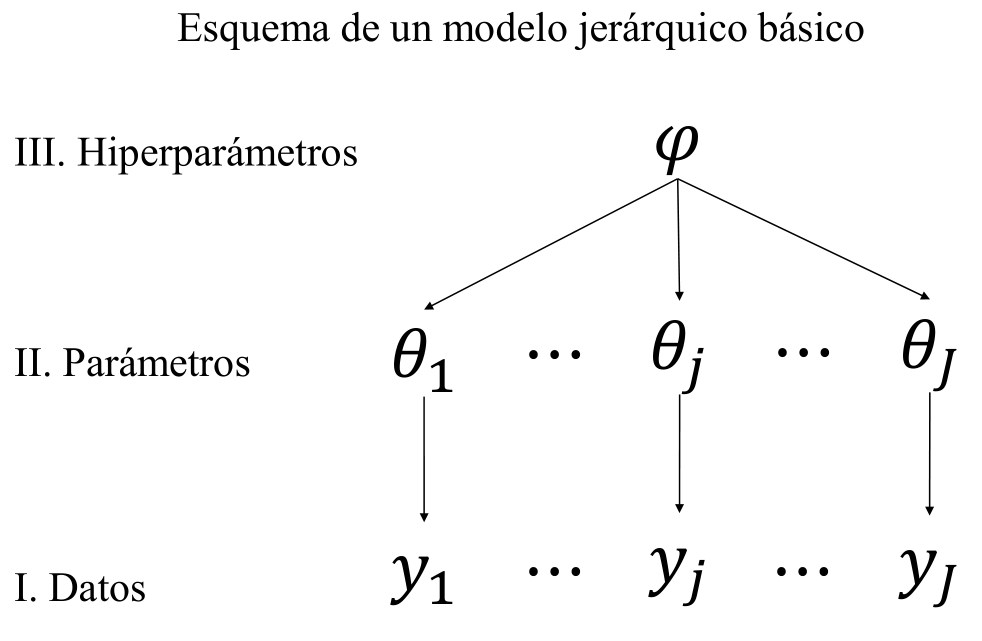
\includegraphics[scale=0.25]{Figs/Bayes/Modelo_Jer}
	\caption{Esquema de un modelo jerárquico básico para $J$ subpoblaciones. Los datos de cada subpoblación $y_j$ son condicionalmente independientes dado un parámetro $\theta_j$. Los parámetros $\theta$ son, a su vez, intercambiables y se modelan condicionalmente independientes dado un hiperparámetro poblacional $\varphi$. Fuente: elaboración propia.}
	\label{fig:Esquema_Modelo_Jer}	
\end{figure}

Un modelo jerárquico aumenta el número de parámetros a estimar al agregar los hiperparámetros. Entonces, tenemos que la distribución inicial de los parámetros depende de un hiperparámetro mismo que, para realizar el aprendizaje bayesiano, deberá tener una distribución \textit{hiperinicial}. El problema consiste en inferir tanto las características de las subpoblaciones, $\theta_j$, como aquellas poblacionales, $\varphi$ \parencite{GP98}: 
\begin{align*}
f(\theta,\varphi|y) & \propto f(y|\theta,\varphi)f(\theta,\varphi) \\
&\propto f(y|\theta)f(\theta|\varphi)f(\varphi) \\
&\propto f(\varphi)\prod\limits_{j=1}^Jf(y_j|\theta_j)\prod\limits_{j=1}^Jf(\theta_j|\varphi) \\
&\propto f(\varphi)\prod\limits_{j=1}^Jf(y_j|\theta_j)f(\theta_j|\varphi)
\end{align*}

\subsection{Regresiones jerárquicas}

En términos de regresiones, los modelos jerárquicos son aquellos en los que los coeficientes también son modelados mediante hiperparámetros estimados con los mismos datos \parencite{GelmanHill06}. Esto permite pensar en regresiones a distintos niveles y con variables grupales, estudios con base en muestreo estratificado e incluso estructuras no necesariamente anidadas. Las ventajas de los modelos jerárquicos hacen que, para algunos investigadores, las regresiones multinivel merezcan ser el enfoque predeterminado \parencite{McElreath15}.\\

\begin{figure}[h]
    \centering
    \begin{subfigure}{0.3\textwidth}
        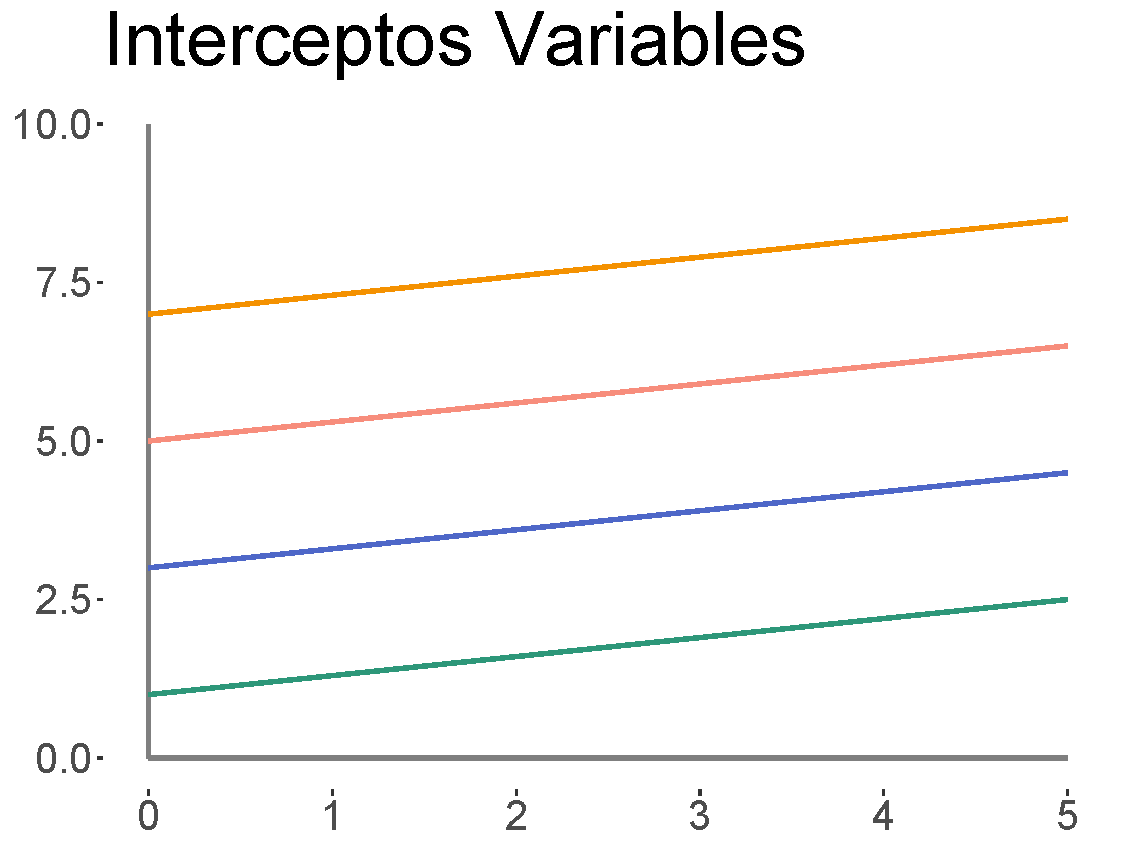
\includegraphics[width=\textwidth]{Figs/Bayes/Interceptos_Variables}
        \label{fig:Ejemplos_Jer_Int_Var}
        \caption{$y_i = \alpha_{j[i]} + \beta x_i$}
    \end{subfigure}
    ~ 
    \begin{subfigure}{0.3\textwidth}
        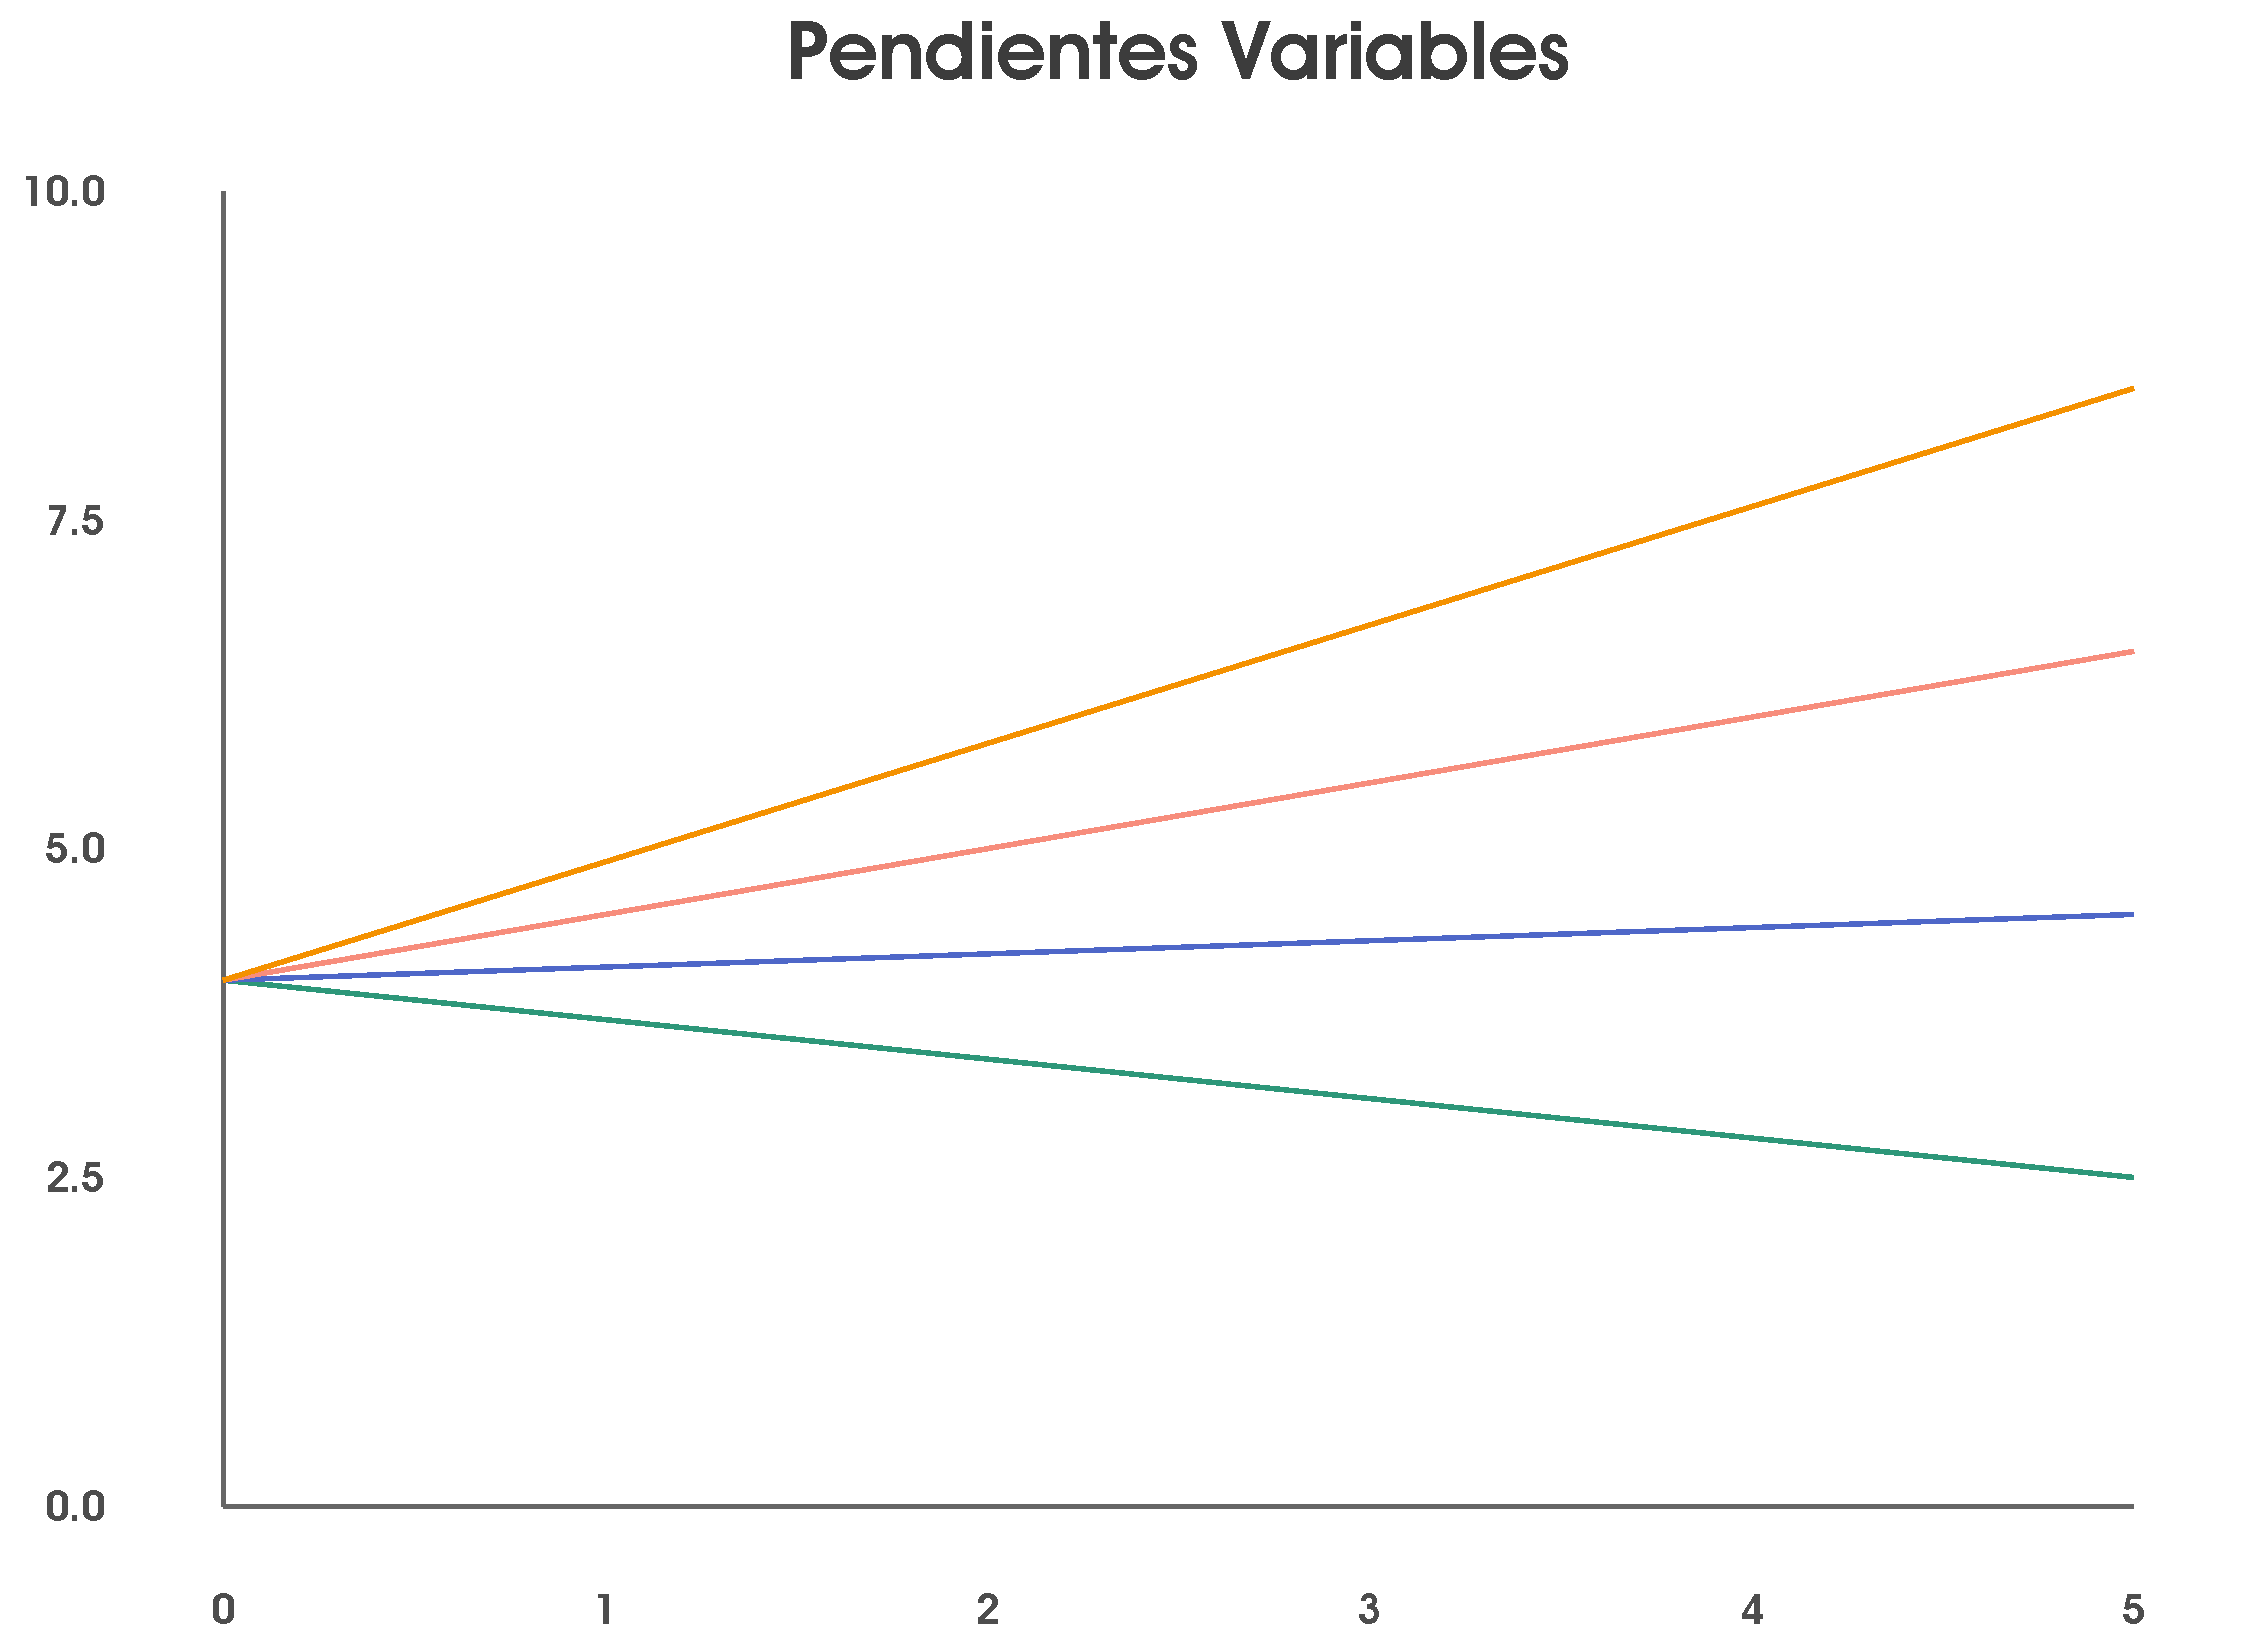
\includegraphics[width=\textwidth]{Figs/Bayes/Pendientes_Variables}
        \label{fig:Ejemplos_Jer_Pend_Var}
        \caption{$y_i = \alpha + \beta_{j[i]} x_i$}
    \end{subfigure}
    ~
    \begin{subfigure}{0.3\textwidth}
        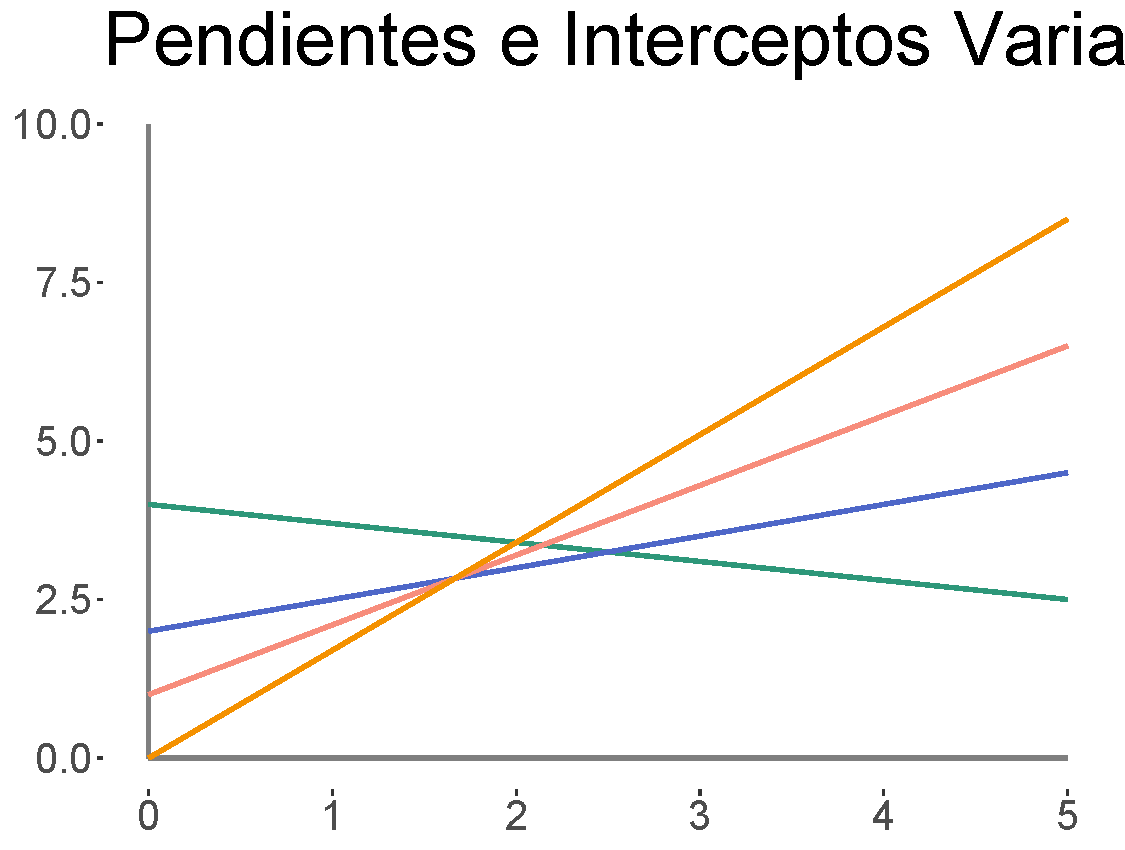
\includegraphics[width=\textwidth]{Figs/Bayes/Pend_e_Inter_Variables}
        \label{fig:Ejemplos_Jer_Pend_Int_Var}
        \caption{$y_i = \alpha_{j[i]} + \beta_{j[i]} x_i$}
    \end{subfigure}
    \caption{Ilustración de los tres tipos generales de modelos jerárquicos. Fuente: elaboración propia con base en la figura (11.1) de \textcite{GelmanHill06}.}\label{fig:Ejemplos_Jer}
\end{figure}

De manera general es posible clasificar las regresiones jerárquicas en tres grandes categorías: interceptos variables, pendientes variables e interceptos y pendientes variables. De manera gráfica estos pueden verse en la \textbf{Figura \ref{fig:Ejemplos_Jer}}. Para presentarlas, supongamos que tenemos $N$ observaciones $\left\lbrace(y_i,x_i,u_{j[i]})\right\rbrace_{i=1}^{N}$ agrupadas en $J$ grupos. Nuestra variable de interés es $Y$, contamos con una variable explicativa a nivel individuo, $X$,  y una a nivel grupo,  $U$.  Debido a que ahora tenemos $J$ grupos, indico con la notación $j[i]$ el grupo al que pertenece el $i$-ésimo individuo. En el \textbf{Cuadro \ref{tbl:Regr_Jer_Lineales}} presento ejemplos esquemáticos de este tipo para modelos lineales en los que $\alpha$ representa el intercepto y $\beta$ la pendiente de la recta; en el caso de los \textit{hipercoeficientes} estos se representan por $a$ y $b$.\\

\begin{table}
\centering
\resizebox{\linewidth}{!}{
\begin{tabular}{l l l l}
Nivel de jerarquía & \textbf{Interceptos variables} & \textbf{Pendientes variables} & \textbf{Interceptos y pendientes variables} \\
\hline 
\\
I. Datos & 
	$\;y_i \sim N(\alpha_{j[i]} + \beta x_i,\sigma_y^2)$ & 
	$\;y_i \sim N(\alpha + \beta_{j[i]} x_i,\sigma_y^2)$ &
	$\;y_i \sim N(\alpha_{j[i]} + \beta_{j[i]} x_i,\sigma_y^2)$\\ 
	\\
	\\
II. Parámetros & 
	$\;\alpha_{j[i]} \sim N(a + b u_{j[i]})$ & 
	$\;\beta_{j[i]} \sim N(a + b u_{j[i]})$ &
	$\;\alpha_{j[i]} \sim N(a_{\alpha} + b_{\alpha} u_{j[i]}, \sigma_{\alpha}^2)$\\
	\\[-1ex] 
	& 
	& 
	&
	$\;\beta_{j[i]} \sim N(a_{\beta} + b_{\beta} u_{j[i]}, \sigma_{\beta}^2)$ \\
	\\
	\\
III. Hiperparámetros & 
	$\;f(\varphi) = f(\beta,\sigma_y^2,a,b,\sigma_{\alpha}^2)$ & 
	$\;f(\varphi) = f(\alpha,\sigma_y^2,a,b,\sigma_{\beta}^2)$ &
	$\;f(\varphi) = f(\sigma_y^2,a_{\alpha},b_{\alpha},\sigma_{\alpha}^2,a_{\beta},b_{\beta},\sigma_{\beta}^2)$\\
\end{tabular}}
\caption{Ejemplos esquemáticos de regresiones jerárquicas lineales. Fuente: elaboración propia.}
\label{tbl:Regr_Jer_Lineales}
\end{table}

Una de las ventajas que tienen los modelos jerárquicos es que cuando se tiene una variable categórica--- a diferencia de lo que sucede en un modelo lineal normal (ver página \pageref{prob_multicolinealidad})--- no es necesario excluir una categoría de referencia. Por el contrario, es posible conservar el intercepto y todas las variables indicadoras dicotómicas con sus respectivos coeficientes. La clave está en que los coeficientes ahora tienen a su vez una distribución que los modela, misma que tiene el efecto de agregar un término a la matriz $X^TX$, lo que la convierte en una matriz invertible y elimina este caso particular de multicolinealidad \parencite{GelmanHill06}. 

\subsubsection*{Regresión logística jerárquica}

Naturalmente, es posible proponer MLG jerárquicos. Por ejemplo, una regresión logística jerárquica con algunas \textit{hiperiniciales} arbitrarias sería la siguiente: 
\begin{align*}
y_i|\alpha_{j[i]},\beta_{j[i]} & \sim Binom(n_i,p_i) \\
ln\left(\dfrac{p_i}{1-p_i}\right) &= \alpha_{j[i]} + \beta_{j[i]} x_i  \\ 
\alpha_{j[i]} & \sim N(a_{\alpha} + b_{\alpha} u_{j[i]}, \sigma_{\alpha}^2) \\ 
\beta_{j[i]} & \sim N(a_{\beta} + b_{\beta} u_{j[i]}, \sigma_{\beta}^2) \\ 
a_{\alpha} \sim N(0,5) \quad & a_{\beta} \sim N(0,5) \quad \sigma_{\alpha} \sim HCauchy(0,1) \\
b_{\alpha} \sim N(0,5) \quad & b_{\beta} \sim N(0,5) \quad \sigma_{\beta} \sim HCauchy(0,1)
\end{align*}

Como puede intuirse, la estructura de un modelo jerárquico crece rápidamente. Sin embargo, recordemos que la \textit{única receta de la inferencia bayesiana} sigue siendo la misma: encontrar la distribución condicional de todas aquellas cantidades de interés cuyo valor desconocemos, dado el valor conocido de las variables observadas. Gracias a las herramientas computacionales este cálculo es posible para modelos cada vez más complejos. En el siguiente capítulo, entonces, discutiré algunos métodos computacionales que permiten este aprendizaje bayesiano. 

	\chapter{Cómputo bayesiano} \label{chap:Cap_MCMC}

De acuerdo con \textcite{Ross10}, los resultados más importantes y más conocidos de la teoría de probabilidad son los llamados teoremas límite, en particular aquellos conocidos como \textit{leyes de los grandes números}. La idea general podemos tomarla de Jakob Bernoulli, el primero en presentar un teorema de este tipo, y estriba en que todos los hombres saben ``por algún instinto de la naturaleza \textit{per se} y sin ninguna instrucción previa, que entre más observaciones hay, menor es el peligro de alejarse del blanco" \parencite{Pulskamp09}. Es decir, si tenemos suficientes realizaciones de un experimento, podemos estimar con mucha precisión aquello que buscamos.\\

Después de varios avances históricos que pueden consultarse en \textcite{Seneta13}, hoy contamos con las leyes débil y fuerte de los grandes números \parencite{Ross10}. Ambas nos dicen que, conforme el tamaño de una muestra aleatoria aumenta, los promedios empíricos convergen a los promedios teóricos. Una manera común de ejemplificar este fenómeno es mediante el lanzamiento sucesivo de monedas. En este caso los volados \textit{simulan} observaciones de una variable aleatoria de ensayos Bernoulli y, al tener una muestra suficientemente grande, se comienza a apreciar la convergencia hacia la probabilidad de éxito.\\ 

Gracias al avance tecnológico, hoy ya no tenemos necesariamente que lanzar volados físicamente sino que los simulamos desde una computadora, a partir de la generación de números pseudoaleatorios, diseñados de manera tal que satisfagan todas las propiedades básicas de números auténticamente aleatorios \parencite{Ross13}. Podemos pedirle a la computadora que simule una gran cantidad de volados \textit{justos} y registre la proporción empírica acumulada de los que cayeron águila. Conforme más aumenta el número de volados, más nos acercamos a 0.5, la proporción teórica. Esto se puede repetir para otras series de volados y el comportamiento es el mismo, como puede apreciarse en la \textbf{Figura \ref{fig:LGN}}. \\

\begin{figure}[h]
	\centering
	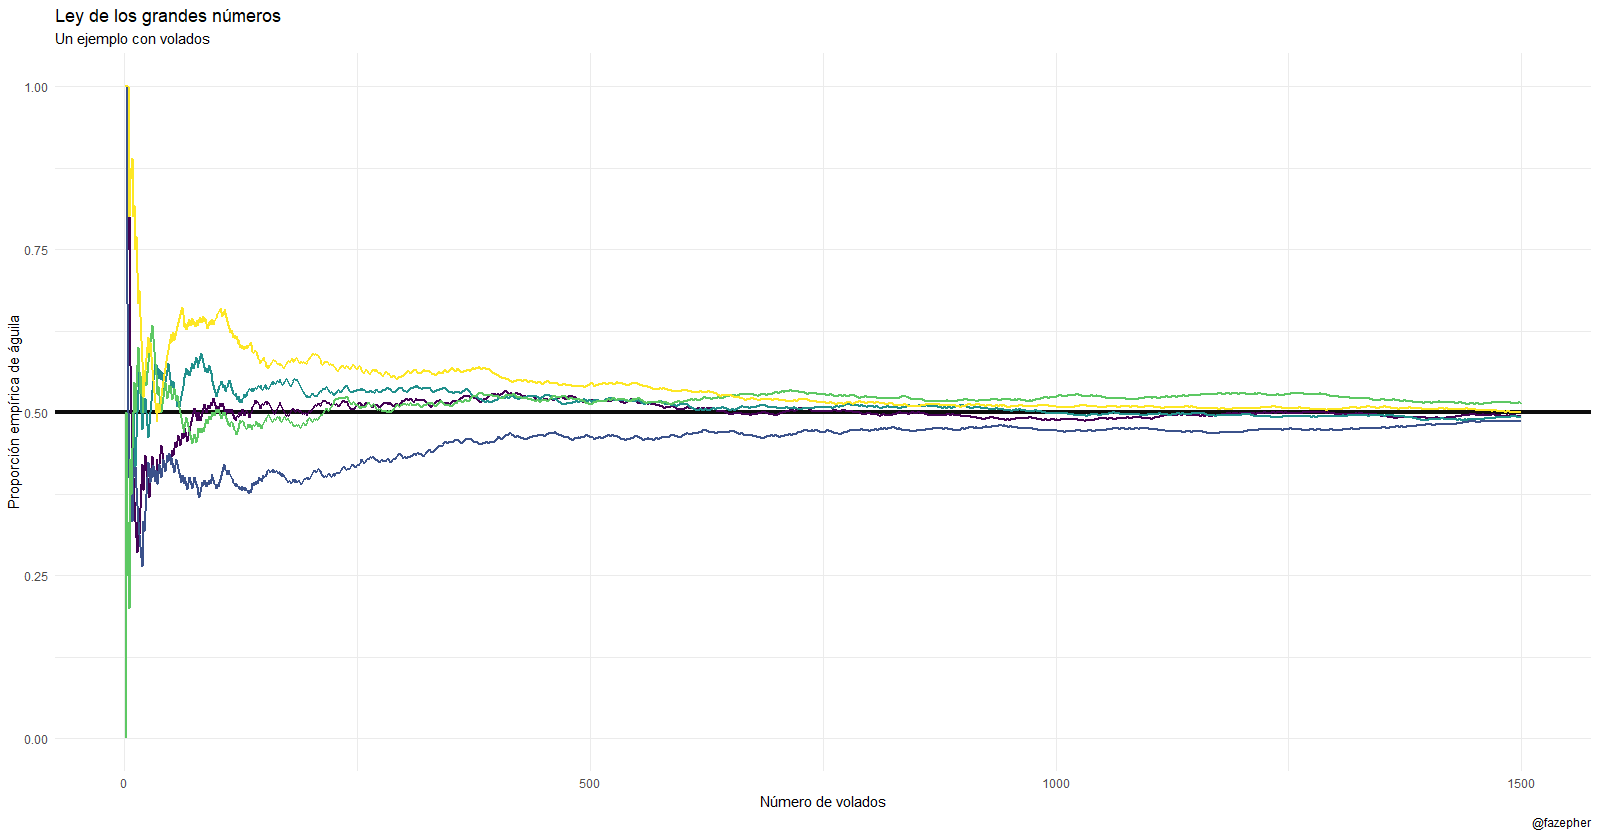
\includegraphics[scale=0.2]{Figs/LGN}
	\caption{Ilustración de las leyes de los grandes números mediante volados simulados por computadora. Conforme el número de volados aumenta, la proporción empírica converge a la proporción teórica. Esto pasa para cada serie de volados. Fuente: elaboración propia.}
	\label{fig:LGN}	
\end{figure}

Es cierto que esta práctica de aprender de un sistema, simulando con muestreo aleatorio no surge con las computadoras \parencite{Owen13}. Ya desde 1812 Laplace había sugerido la posibilidad de estimar empíricamente el valor de $\pi$ mediante el llamado problema de la aguja de Buffon \parencite{Ragheb13}. Sin embargo, como el ejemplo de los volados muestra, sí han sido las computadoras las que han potenciado la utilidad de los métodos de simulación. ¿Cuánto hubiéramos tardado en lanzar los 7,500 volados que la computadora simuló al instante? Más aún, esta capacidad computacional consolidó la utilidad de la estadística bayesiana. ¡Y pensar que todo empezó con una guerra y un juego de solitario!, como explico a continuación.

\section{Monte Carlo} 

La simulación por computadora ha permitido el desarrollo de la estadística bayesiana, particularmente desde la década de los 90 del siglo pasado \parencite{RobertCasella11}. Sin embargo, la semilla de este desarrollo ya había sido plantada medio siglo antes desde el terreno de la física, desafortunadamente a causa de la Segunda Guerra Mundial, por los científicos del laboratorio de Los Alamos, encargados del proyecto Manhattan y el desarrollo de más armas de fisión nuclear.\\

Uno de esos científicos fue un matemático polaco-estadounidense llamado Stanislaw Ulam. En 1946, aburrido convaleciendo por una enfermedad, comenzó a preguntarse sobre la probabilidad de ganar en un juego de solitario. Después de mucho batallar con los cálculos de combinatoria se planteó si no sería más práctico estimarla simulando muchas partidas en una de las primeras computadoras electrónicas. Y ahí surgió el eureka: ¿por qué no hacer lo mismo para los problemas de física nuclear en los que estaban trabajando en Los Alamos? \parencite{Eckhardt87}. Al igual que las partidas de solitario, podrían simular muchas realizaciones de los procesos físicos bajo estudio y estimar los resultados más probables.\\ 

Stan compartió su idea con John von Neumann quien, sorprendido y emocionado con la idea, le envió una carta a Richard Richtmayer--- el líder del equipo en Los Alamos--- con todos los cálculos necesarios para llevar a cabo el proyecto \parencite{vonNeumann47}. El método fue rápidamente adoptado por todos en Los Alamos, tanto que otro físico, Nicholas Metropolis, sugirió llamarlo \textit{Monte Carlo}, bromeando sobre un tío apostador de Stan, que vivía pidiendo prestado dinero porque ``simplemente tenía que ir a Monte Carlo" \parencite{Metropolis87}. Después de un arduo trabajo, el método pareció funcionar--- gracias en buena medida al trabajo de programación de Klara von Neumann \parencite{Haigh14}--- y el propio Metropolis publicó, junto con Stan, un primer paper presentándolo a grandes rasgos \parencite{MetropolisUlam49}.\\

De manera concreta, el método es la conjunción de la simulación con la ley de los grandes números. Las cantidades que requerían calcular eran valores esperados de la siguiente forma: 
\begin{equation}
\label{eq:IntegralMC}
h^\star = \E{h(Z)}=\int\limits_\mathcal{Z} h(z)f(z)dz ,
\end{equation} 
donde $h$ es una función de interés y $f(z)$ es la distribución de probabilidad sobre las \textit{configuraciones} $z$ en las que podía encontrarse el sistema físico. El gran problema era--- y sigue siendo--- que estas integrales típicamente no pueden calcularse ni analíticamente ni por métodos numéricos tradicionales. Sin embargo, si se tiene una muestra aleatoria de valores de $Z$ provenientes de su distribución $f$, se puede aproximar $h^\star$ con el promedio empírico, que en este contexto se conoce como \textit{estimador de Monte Carlo}: 
\begin{equation*}
h^\star \approx \hat{h} = \sum\limits_{i=1}^N \dfrac{h(z_i)}{N}
\end{equation*}

Entonces, los científicos en Los Alamos se dedicaron a encontrar algoritmos eficientes para obtener una muestra aleatoria de variables provenientes de diferentes distribuciones $f$.\\ 

Lo importante para este trabajo es que este es exactamente el mismo probelma que se tiene en la aplicación de la estadística bayesiana y que hizo que por décadas--- por no decir siglos--- fuera poco menos que imposible llevar a cabo análisis bayesianos no triviales, como ya anticipa en \ref{sec:Prob_Analitico}. Muchas de las integrales que surgen en la estadística bayesiana no pueden ser calculadas de manera analítica. El ejemplo más frecuente es la constante normalizadora del teorema de Bayes. ¿Cómo aplicar el teorema si el denominador no puede ser calculado?\\ 

No obstante, la forma de \eqref{eq:IntegralMC} permite llevar a cabo una gran variedad de \textit{resúmenes inferenciales} \parencite{GP97}. La posibilidad de realizar las correspondientes \textit{integraciones por Monte Carlo} hace que, en la práctica, exista una dualidad entre una distribución o densidad y una muestra proveniente de ella \parencite{SmithGelfand92}. La única receta de la inferencia bayesiana--- ver la página \pageref{receta_bayesiana}---, en la práctica se convierte en obtener una muestra aleatoria de la distribución posterior lo suficientemente grande para, con ella, estimar por Monte Carlo los resúmenes inferenciales requeridos.\\

Hay varios métodos de simulación de variables aleatorias que permiten obtener muestras aleatorias independientes y calcular un estimador de Monte Carlo. Entre los más mencionados podemos encontrar el método de inversión, el de aceptación y rechazo o el muestreo por importancia \parencites{Ross13,RobertCasella10}. Sin embargo, los físicos de Los Alamos pronto se dieron cuenta que, en lugar de buscar realizar directamente simulaciones independientes, era más práctico hacer simulaciones secuenciales que dependieran entre sí. 

\section{MCMC}

La forma de realizar simulaciones correlacionadas que logren simular de manera más eficiente que los métodos directos tradicionales de aceptación y rechazo o muestreo por importancia es utilizar \textit{cadenas de Markov}.

\dfn{\textbf{Cadena de Markov}\\
\label{def:Cadena_Markov}
Una \textit{cadena de Markov} $\left\lbrace Z^{(n)}, \, n = 0, 1, 2,\dots \right\rbrace$ es una secuencia de variables aleatorias tales que satisfacen la siguiente \textit{propiedad de Markov} para toda $n$
\begin{equation*}
Z^{(n+1)}| Z^{(n)}, \dots, Z^{(0)} \sim Z^{(n+1)}| Z^{(n)} \sim p(z^{(n+1)}|z^{(n)})
\end{equation*}
}
Si llamamos \textit{estados} a los eventos que suceden en la cadena en cada punto en el tiempo, podemos decir que la distribución condicional del estado futuro de una cadena de Markov dada toda su historia depende exclusivamente del estado presente y no de los estados anteriores. Dicho de otra forma, \textit{el futuro es independiente del pasado, dado el presente}. La distribución condicional se llama \textit{kernel de transición}, mismo que normalmente es también independiente del índice $n$ y depende exclusivamente del estado actual y el estado futuro. Esta propiedad se llama \textit{homogeneidad} en el tiempo y permite simplificar la notación a $p(\tilde{z}|z)$.\\ 

La teoría de cadenas de Markov determina las condiciones bajo las cuales existen teoremas límites al estilo de las leyes de los grandes números y que en este contexto se conocen como \textit{ergódicos}. Esta teoría escapa los objetivos particulares de la tesis pero, si es de interés para el lector, algunas referencias útiles son \textcites{Rincon12,Neal93,Ross96,TaylorKarlin84}. Baste decir por ahora que, bajo ciertas condiciones, sabemos que la distribución de $Z^{(n)}$ converge a una distribución límite conforme $n$ tiende a infinito. Más aún, los \textit{promedios ergódicos}--- es decir los promedios acumulados de la cadena--- también convergen al valor esperado de la distribución límite. Esto se puede expresar matemáticamente como sigue:
\begin{subequations}\label{eq:Teo_Erg}
\begin{align}
Z^{(N)} &\xrightarrow[N\rightarrow\infty]{\mathcal{D}} Z, \quad Z \sim f(z) \label{eq:Teo_Erg_Conv_D} \\
\dfrac{1}{N}\sum\limits_{n=1}^N h\left(z^{(n)}\right) &\xrightarrow[N\rightarrow\infty]{} \mathbb{E}_{f}[h(z)]
\label{eq:Teo_Erg_Conv_Prom}
\end{align}
\end{subequations}

Esto da lugar a los métodos de \textit{Markov Chain Monte Carlo} o MCMC en los que el objetivo es construir una cadena de Markov que satisfaga las condiciones necesarias y cuya distribución límite sea la distribución de la cual se quiere simular. Así, después de $N$ transiciones de la cadena, la simulación convergería a la distribución objetivo y se podría estimar la cantidad de interés $h^\star$ mediante el estimador de MCMC: 

\begin{equation*}
h^\star \approx \hat{h} = \sum\limits_{n=1}^N \dfrac{h\left(z^{(n)}\right)}{N}
\end{equation*}

\subsection{Metropolis Hastings}

 El primero de estos métodos MCMC fue propuesto por las parejas de esposos Arianna y Marshall Rosenbluth y Augusta y Edward Teller junto con el propio Nicholas Metropolis en el \textit{Journal of Chemical Physics} \parencite{Metropolis53}. Se conoce como el algoritmo de Metropolis, aunque hay quienes creen que en realidad el trabajo más fuerte lo hicieron el resto de los autores por lo que debería llamarse el algoritmo de Rosenbluth-Teller \parencite{Gubernatis05}. Casi 20 años después, el estadístico canadiense Wilfred Keith Hastings lo generalizó \parencite{Hastings70}, por lo que podemos hablar de algoritmos de Metropolis Hastings o MH.

\subsubsection*{Balance detallado, la clave de MH}
 
Las cadenas de Markov para MH requieren ser homogéneas en el tiempo y que sea posible llegar a cualquier estado en un número finito de transiciones, algo que se conoce como \textit{irreducibilidad}. Si además el kernel de transición satisface la siguiente \textit{ecuación de balance detallado} para alguna distribución $f$, se dice que es \textit{reversible} y podemos aplicar el teorema ergódico.
\begin{equation}
\label{eq:Balance_Detallado}
f(z)p(\tilde{z}|z)=f(\tilde{z})p(z|\tilde{z})
\end{equation}

El algoritmo de Metropolis Hastings busca construir cadenas de Markov homogéneas, irreducibles y reversibles que tengan como distribución límite a la distribución objetivo. ¿Cómo hacerlo? Para ello analicemos lo que la reversibilidad implica de manera intuitiva.\\

Siguiendo la argumentación de \textcite{ChibGreenberg95}, \eqref{eq:Balance_Detallado} refleja que hay un balance entre las probabilidades de la cadena de estar en diferentes estados, de ahí el nombre. Supongamos que no se cumpliera la reversibilidad para algún kernel $q(\tilde{z}|z)$. Entonces, sin pérdida de generalidad, para algunos estados pasaría que:
\begin{equation}
\label{eq:Inbalance_Detallado}
\dfrac{f(z)}{f(\tilde{z})}>\dfrac{q(z|\tilde{z})}{q(\tilde{z}|z)}
\end{equation}

De manera un poco informal, tenemos que el miembro izquierdo de la desigualdad refleja las probabilidades relativas ``necesarias'' entre estar en el estado $z$ y el estado $\tilde{z}$. El miembro derecho, por su parte, indica las probabilidades relativas de transitar a dichos estados bajo el kernel de transición de la cadena. La desigualdad indica que la cadena estaría transitando a $\tilde{z}$ más de lo necesario y, equivalentemente, transitaría a $z$ menos de lo necesario.\\ 

Para conseguir el balance requerido para aplicar el teorema ergódico, necesitamos hacer una \textit{corrección de Metropolis} al kernel de transición, reduciendo el número relativo de veces que la cadena transite de $z$ a $\tilde{z}$ y aumentando el número relativo de transiciones de $\tilde{z}$ a $z$. La forma de hacer la corrección es comenzar con un kernel, $q(\tilde{z}|z)$, que \textit{proponga} un estado y agregar una \textit{probabilidad de aceptación} de la propuesta, $\alpha(\tilde{z};z)$. Si es rechazada, la cadena permanece en el mismo estado, reduciendo a la vez el número de transiciones hacia estados sobremuestreados y aumentando el número relativo de veces que estamos en el estado originalmente submuestreado. Estos dos pasos constituyen un kernel de transición de Metropolis Hastings de la siguiente forma: 
\begin{align*}
p_{MH}(\tilde{z}|z) &= q(\tilde{z}|z)\alpha(\tilde{z};z) \quad z \neq \tilde{z} \\
p_{MH}(z|z) &= 1 - \int\limits_{\tilde{\mathcal{Z}}} p_{MH}(\tilde{z}|z)d\tilde{z}
\end{align*}

Queremos que el kernel $p_{MH}$ satisfaga \eqref{eq:Balance_Detallado}, entonces:
\begin{equation*}
f(z)p_{MH}(\tilde{z}|z)=f(\tilde{z})p_{MH}(z|\tilde{z}) \quad \Leftrightarrow \quad f(z)q(\tilde{z}|z)\alpha(\tilde{z};z)=f(\tilde{z})q(z|\tilde{z})\alpha(z;\tilde{z}) 
\end{equation*}

De acuerdo a nuestra desigualdad supuesta en \eqref{eq:Inbalance_Detallado}, las transiciones de $\tilde{z}$ a $z$ se dan demasiado poco, por lo que deberíamos siempre aceptar este tipo de transiciones a fin de corregir el submuestreo. Tomemos entonces $\alpha(z;\tilde{z}) = 1$ y observemos que $\alpha(\tilde{z};z)$ queda determinada de tal forma que logremos el balance necesario: 
\begin{equation*}
\alpha(\tilde{z};z)=\dfrac{f(\tilde{z})q(z|\tilde{z})}{f(z)q(\tilde{z}|z)}
\end{equation*}

Si la desigualdad \eqref{eq:Inbalance_Detallado} fuera en el sentido contrario, i.e. $f(\tilde{z})q(z|\tilde{z})>f(z)q(\tilde{z}|z)$, los roles de las probabilidades de aceptación se invertirían, por lo que de manera general tenemos que 
\begin{equation}
\label{eq:Proba_Aceptar_MH}
\alpha(\tilde{z};z)=min\left\lbrace\dfrac{f(\tilde{z})q(z|\tilde{z})}{f(z)q(\tilde{z}|z)},1\right\rbrace
\end{equation}

La utilidad de MH para la estadística bayesiana está en la forma de la probabilidad de aceptación en \eqref{eq:Proba_Aceptar_MH}. Como la distribución objetivo se encuentra tanto en el denominador como en el numerador, no se requiere completa sino basta con conocerla salvo por una constante de proporcionalidad que desaparezca al realizar el cociente. Esta situación es exactamente la que impera en la aplicación de la estadística bayesiana. Recordemos el resumen del aprendizaje bayesiano en \eqref{eq:Bayes_Prop}, \textit{la posterior es proporcional a la inicial por la verosimilitud}: 
\begin{equation*}
f(\theta|y) \propto L(\theta)f(\theta).
\end{equation*}

Por esto, para simular valores de una distribución posterior $f(\theta|y)$ mediante MH solo necesitamos la distribución inicial $f(\theta)$, la verosimilitud $L(\theta)=f(y|\theta)$ y un kernel de propuestas $q(\tilde{\theta}|\theta)$, siguiendo el \textbf{Algoritmo \ref{alg:MH}}. Hay una última consideración que debe tenerse en cuenta y es que la posterior sea propia; si se inició con una inicial impropia es posible que la posterior no pueda integrar a 1, lo que haría que el algoritmo fallara \parencite{RobertCasella10}.\\

\begin{algorithm}
\DontPrintSemicolon
Valor inicial arbitrario o simulado $\theta^{(0)}$\;
\For{$n \leftarrow 1$ \KwTo $N$}{
$\theta \leftarrow \theta^{(n-1)}$\;
$\tilde{\theta} \sim q(\tilde{\theta}|\theta)$\;
$\alpha(\tilde{\theta};\theta) \leftarrow min\left\lbrace\dfrac{f(y|\tilde{\theta})f(\tilde{\theta})q(\theta|\tilde{\theta})}{f(y|\theta)f(\theta)q(\tilde{\theta}|\theta)},1\right\rbrace$\;
$u \sim U[0,1]$ \;
\eIf{$u \leq \alpha(\tilde{\theta};\theta)$}{
	$\theta^{(n)} \leftarrow \tilde{\theta}$\;
	}{
	$\theta^{(n)} \leftarrow \theta $\;
	}
}

\caption{Metropolis Hastings para el aprendizaje bayesiano \label{alg:MH}}
\end{algorithm}

\subsubsection*{\textit{Random Walk Metropolis}}

Si la posterior es propia, entonces el mayor problema, claro está, es el de encontrar un kernel de propuestas conveniente. Una alternativa son aquellos que exploran progresivamente el espacio de estados de manera local. Estos se conocen como \textit{Random Walk Metropolis} o RWM \parencite{RobertCasella10}. De hecho, el algoritmo inicial de \textcite{Metropolis53} era de este tipo, usando una distribución uniforme en una vecindad del estado actual; pero también se pueden usar otras distribuciones, como una normal o una $t$ de Student centrada en dicho estado. \textcite{Robert15} hace la analogía con alguien que para ver una pintura en un cuarto oscuro tiene que ir alumbrando el cuadro con una antorcha, iluminando secuencialmente diferentes segmentos del lienzo.\\

Estos kérneles de caminata aleatoria son \textit{simétricos}--- esto es,  $q(\tilde{\theta}|\theta) = q(\theta |\tilde{\theta})$--- lo que simplifica los cálculos de probabilidades de aceptación:
\begin{equation*}
\alpha_{RWM}(\tilde{\theta};\theta)=min\left\lbrace\dfrac{f(\tilde{\theta}|y)q(\theta|\tilde{\theta})}{f(\theta|y)q(\tilde{\theta}|\theta)},1\right\rbrace = min\left\lbrace\dfrac{f(\tilde{\theta}|y)}{f(\theta|y)},1\right\rbrace
\end{equation*}

Un ejemplo trivial puede ayudar a visualizar cómo funcionan. Supongamos que quisiéramos simular de una posterior que, en realidad, es una normal bivariada cuyas marginales son normales estándar. Un posible kernel de transición sería una distribución uniforme en un rectángulo de $3$ de lado centrado en el estado actual de la cadena, por lo que tendríamos un kernel simétrico y un algoritmo de \textit{Random Walk Metropolis}.\\ 

Podemos ver cómo se va explorando el espacio de estados en la \textbf{Figura \ref{fig:RWM}}. Cuando una de las propuestas es rechazada, esta se marca como una tache. Empezando en un punto alejado del origen, la cadena comienza a acercarse a la región de mayor densidad. En el fondo--- como quedará más claro después--- encontrar esta \textit{región crítica} y explorarla es el objetivo de un algoritmo de integración por MCMC \parencites{Neal93,Betancourt17}. Con tan solo 2,500 iteraciones la cadena ya la recorrió y los valores que alejarían a la cadena de la misma son normalmente rechazados. Podemos ver también cómo los promedios ergódicos van acercándose a $0$ para ambas variables.\\

\begin{figure}[h]
    \centering
    \begin{subfigure}{0.3\textwidth}
        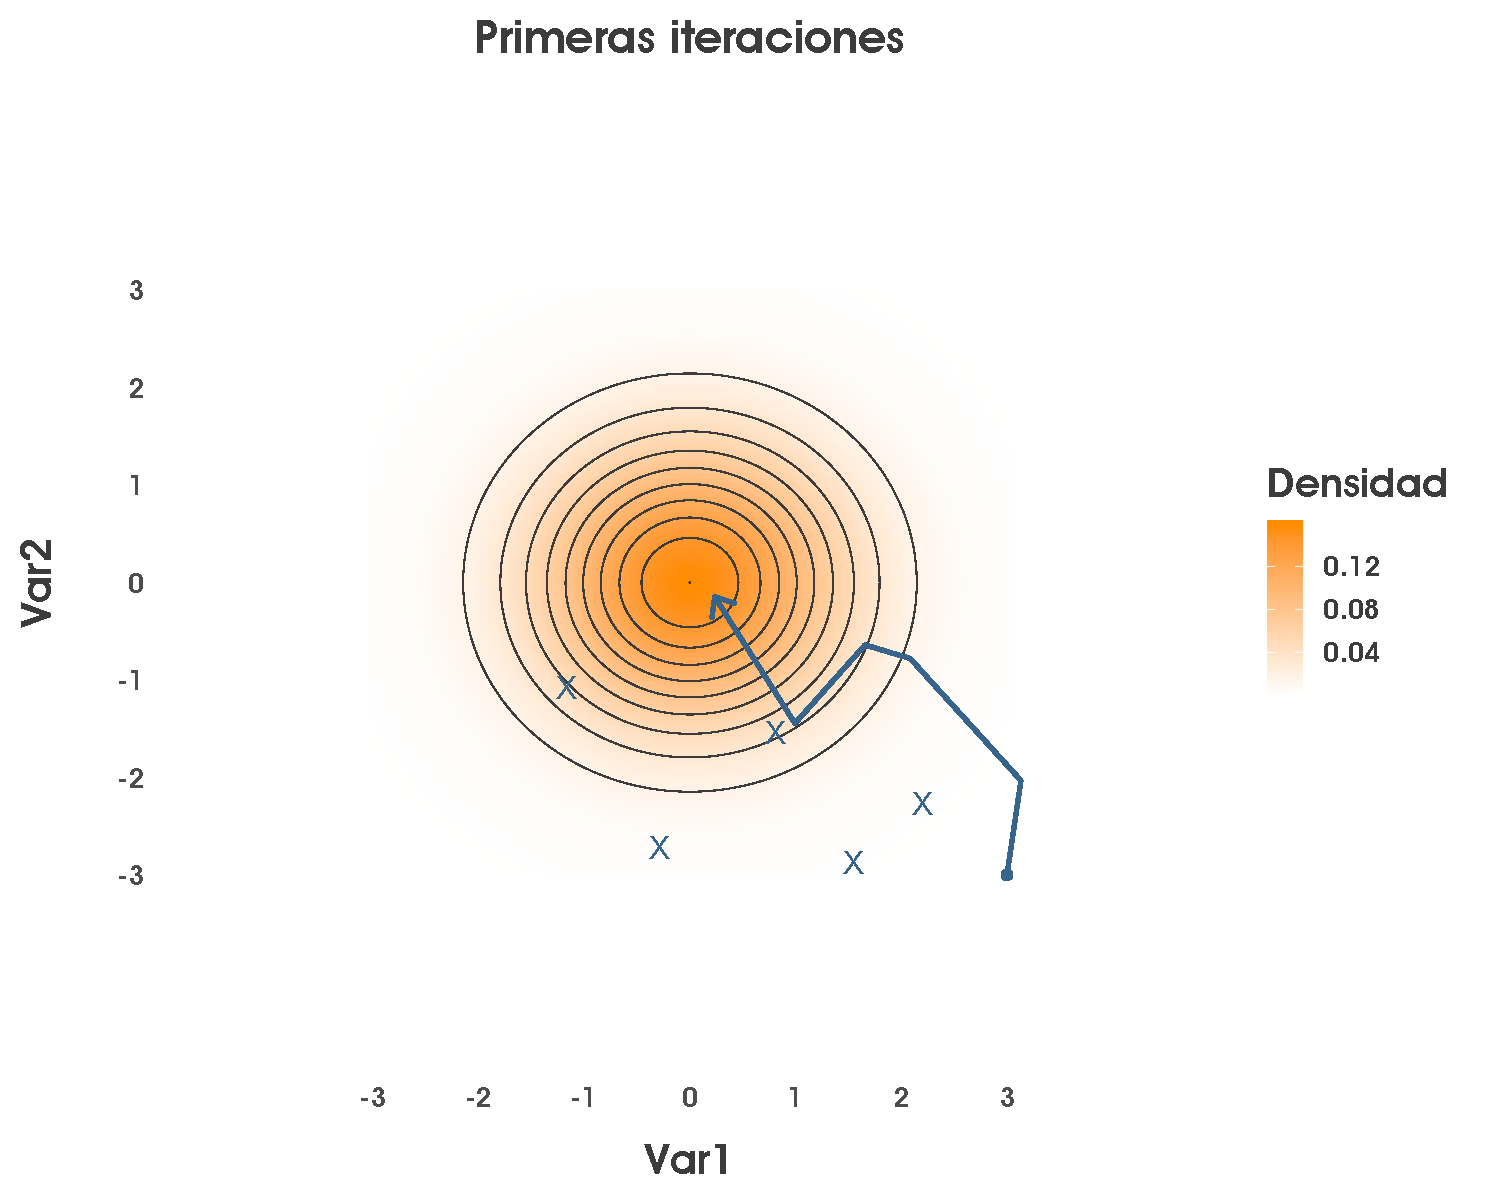
\includegraphics[width=\textwidth]{Figs/Bayes/Ejemplo_RWM_A}
        \caption{La cadena empieza lejos de las zonas de mayor densidad y se va acercando a ellas. Las taches representan propuestas rechazadas.}
    \end{subfigure}
    ~ 
    \begin{subfigure}{0.3\textwidth}
        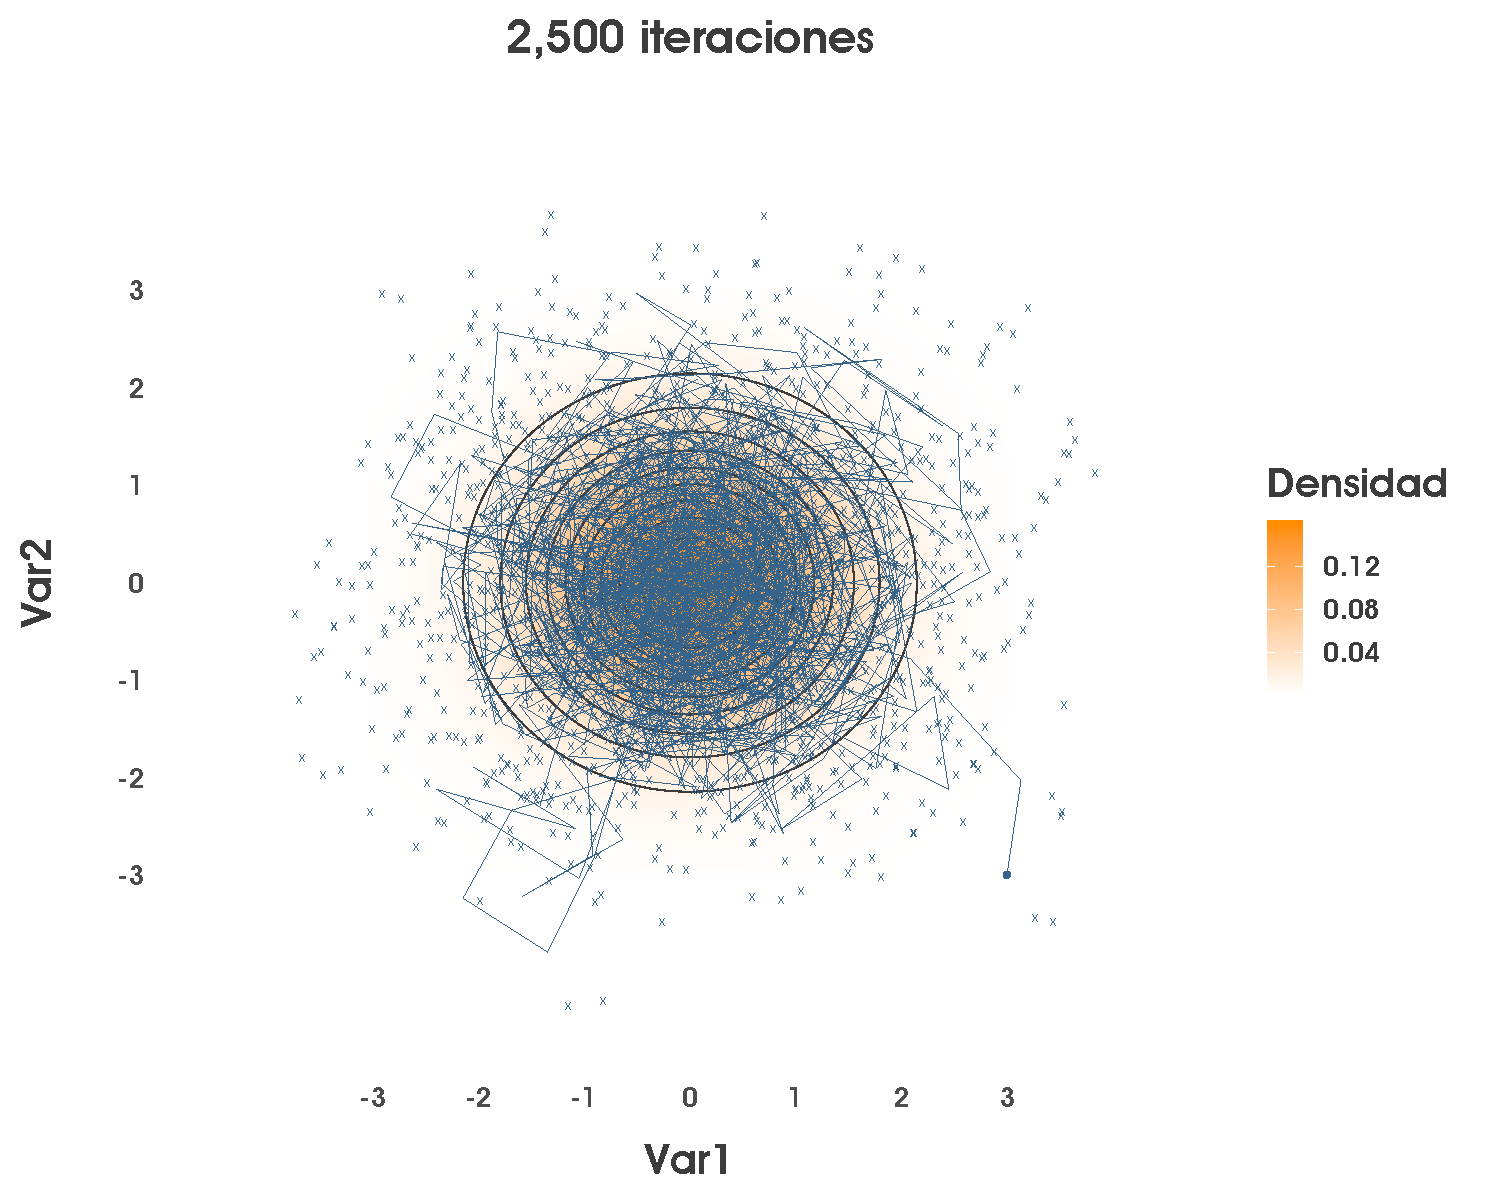
\includegraphics[width=\textwidth]{Figs/Bayes/Ejemplo_RWM_B}
        \caption{Después de 2,500 iteraciones, la cadena explora ya la región crítica. Los valores fuera de ella normalmente son rechazados.}
    \end{subfigure}
    ~
    \begin{subfigure}{0.3\textwidth}
        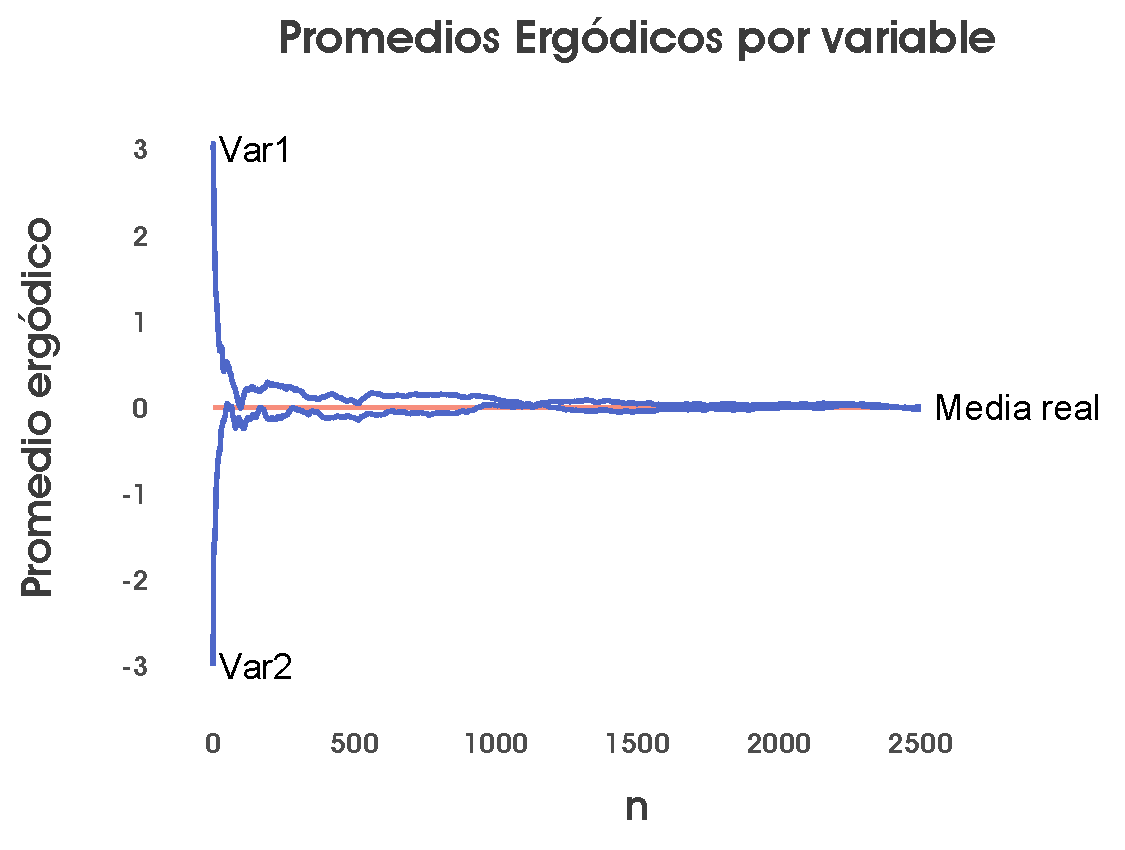
\includegraphics[width=\textwidth]{Figs/Bayes/Ejemplo_RWM_C}
        \caption{Los promedios ergódicos van convergiendo a las medias teóricas.}
    \end{subfigure}
    \caption{Ilustración de una cadena de Metropolis Hastings simulando de una normal bivariada sin correlación mediante una implementación de \textit{Random Walk Metropolis}. Fuente: elaboración propia.}\label{fig:RWM}
\end{figure}

Pero la pregunta permanece, ¿cómo determinar el kernel de propuestas? ¿Por qué usar $3$ como lado y no $0.5$? ¿Qué hubiera pasado en ese caso? Podemos observarlo en la \textbf{Figura \ref{fig:RWM2}}. El rectángulo de propuestas es más pequeño y eso tiene dos efectos: hay menos propuestas rechazadas pero la cadena avanza más lentamente. Vemos cómo aún después de las mismas 2,500 iteraciones la cadena no ha explorado por completo el área de mayor densidad y los promedios ergódicos apenas comienzan a converger.\\ 

\begin{figure}[h]
    \centering
    \begin{subfigure}{0.3\textwidth}
        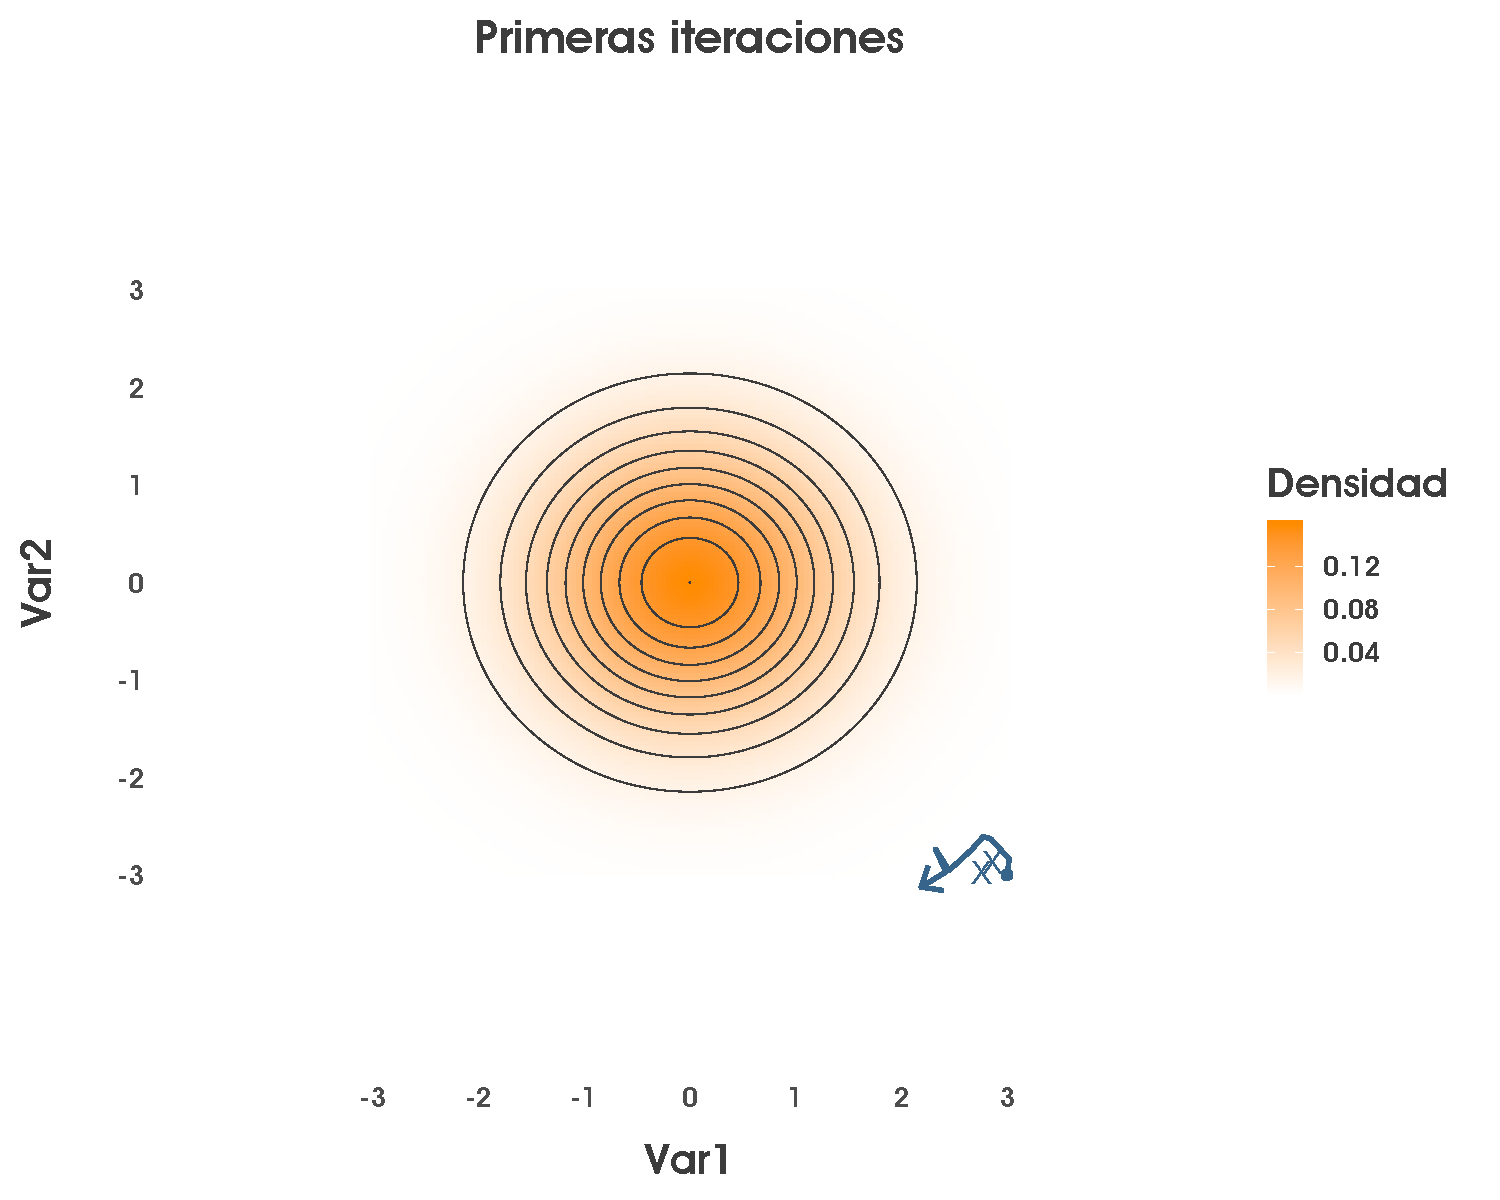
\includegraphics[width=\textwidth]{Figs/Bayes/Ejemplo2_RWM_A}
        \caption{La cadena empieza lejos de las zonas de mayor densidad y avanza lentamente. Las taches representan propuestas rechazadas.}
    \end{subfigure}
    ~ 
    \begin{subfigure}{0.3\textwidth}
        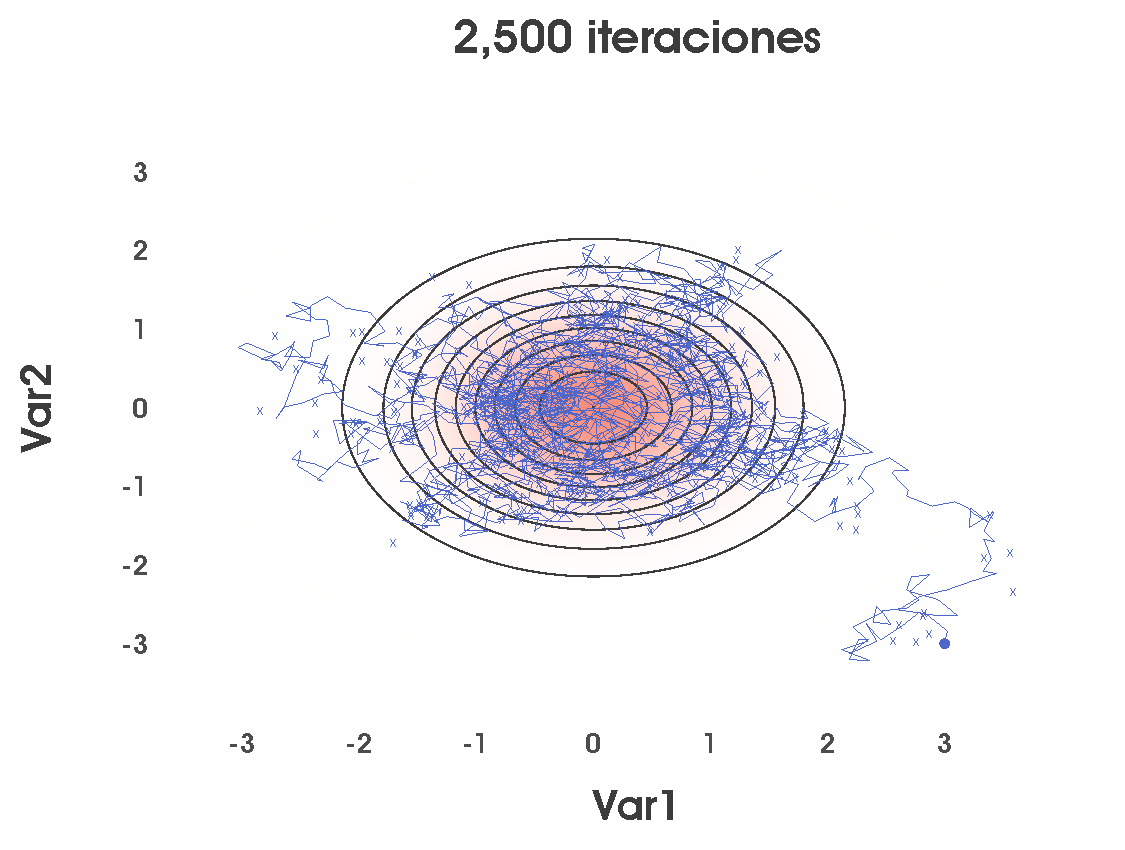
\includegraphics[width=\textwidth]{Figs/Bayes/Ejemplo2_RWM_B}
        \caption{Después de 2,500 iteraciones, la cadena no ha explorado la región crítica, aunque hay menos propuestas rechazadas.}
    \end{subfigure}
    ~
    \begin{subfigure}{0.3\textwidth}
        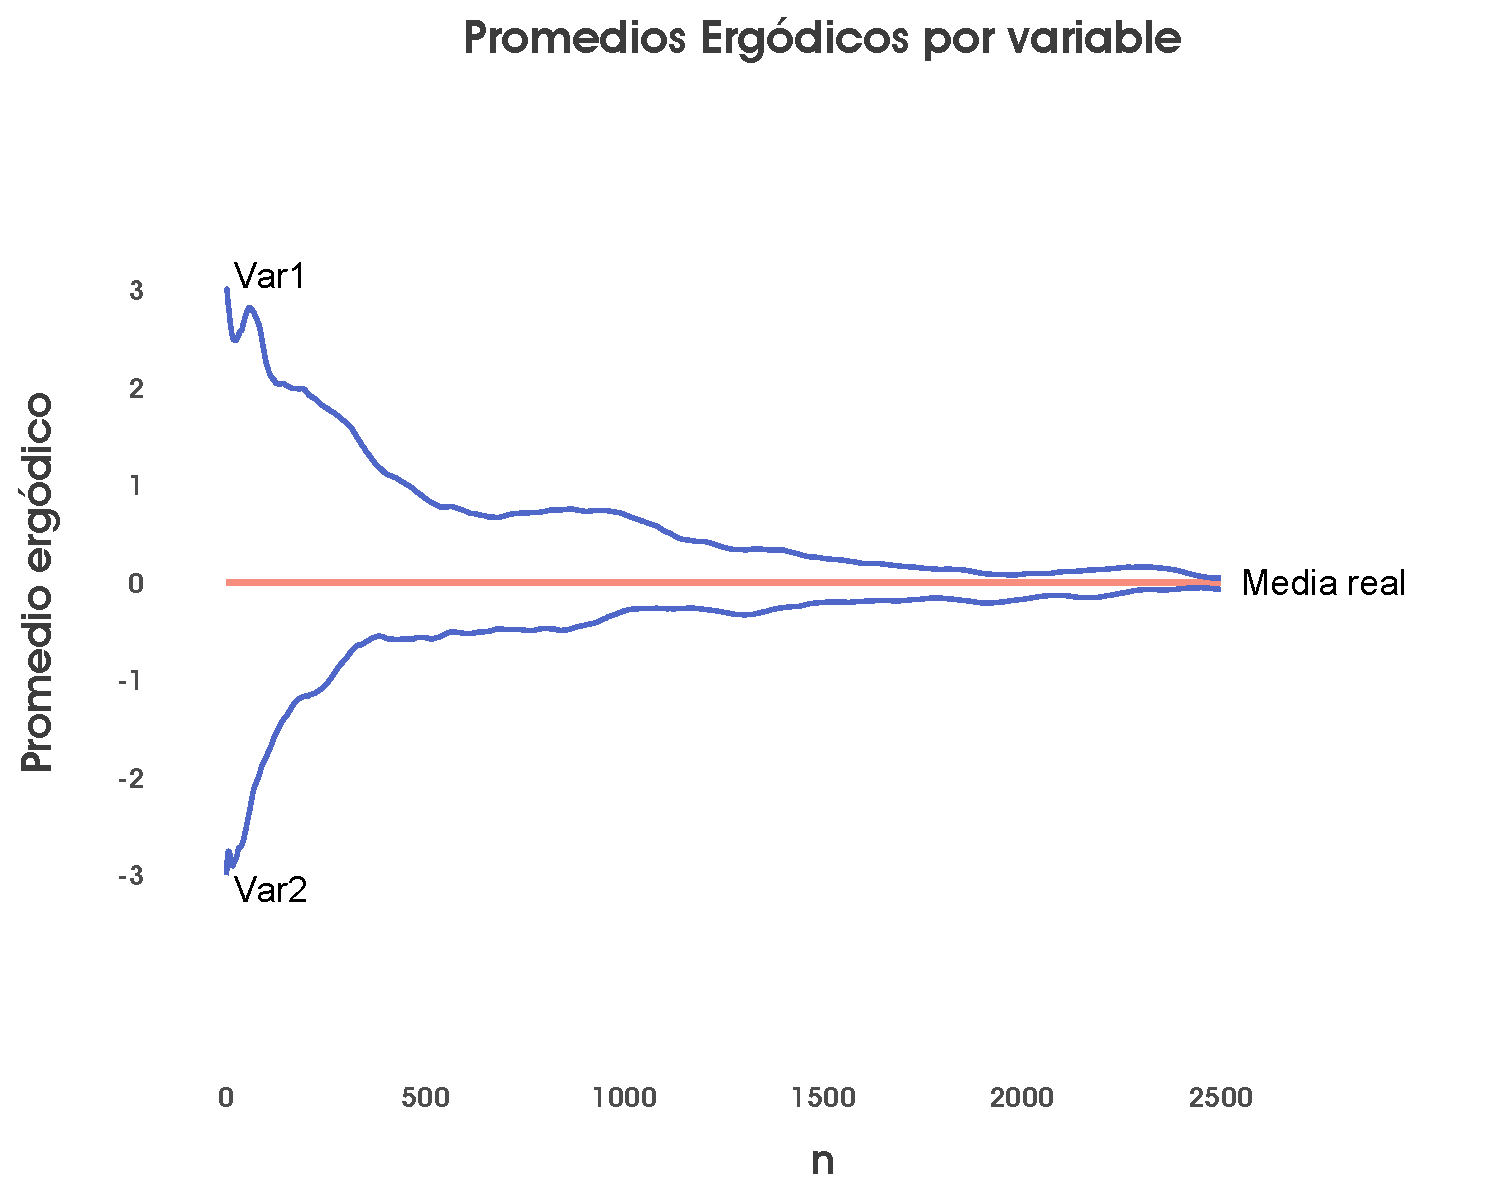
\includegraphics[width=\textwidth]{Figs/Bayes/Ejemplo2_RWM_C}
        \caption{Los promedios ergódicos tardan en converger.}
    \end{subfigure}
    \caption{Ilustración de una cadena de Metropolis Hastings simulando de una normal bivariada sin correlación mediante una implementación de \textit{Random Walk Metropolis} con un kernel de propuestas estrecho. Fuente: elaboración propia.}\label{fig:RWM2}
\end{figure}

El rectángulo más amplio propone valores que se alejan de la región crítica, mismos que tienden a ser rechazados. Sin embargo, también permite proponer valores más distantes del punto actual, lo que en este caso hace que la cadena avance rápidamente. El rectángulo más pequeño avanza más bien ``lento pero seguro''... quizás demasiado lento. Ambas cadenas convergerán, pero este ejemplo ilustra uno de los principales problemas de los algoritmos de MH, en general. Elegir un kernel de propuestas eficiente no es sencillo. Si la escala del kernel es demasiado pequeña, los saltos son demasiado pequeños y la cadena avanza demasiado lento. Si la escala es demasiado grande, corremos el riesgo de que la cadena rechace casi todas las propuestas y quede ``atorada'' en algún lugar; si la cadena repite el mismo valor varias veces seguidas, también alenta su avance. Debe haber un justo medio entre ambos extremos. Esto podemos verlo comparando el comportamiento de tres kérneles cuando intentan simular normales ahora altamente correlacionadas, en la \textbf{Figura \ref{fig:RWM_Corr}}.\\ 

\begin{figure}[h]
    \centering
    \begin{subfigure}{0.3\textwidth}
        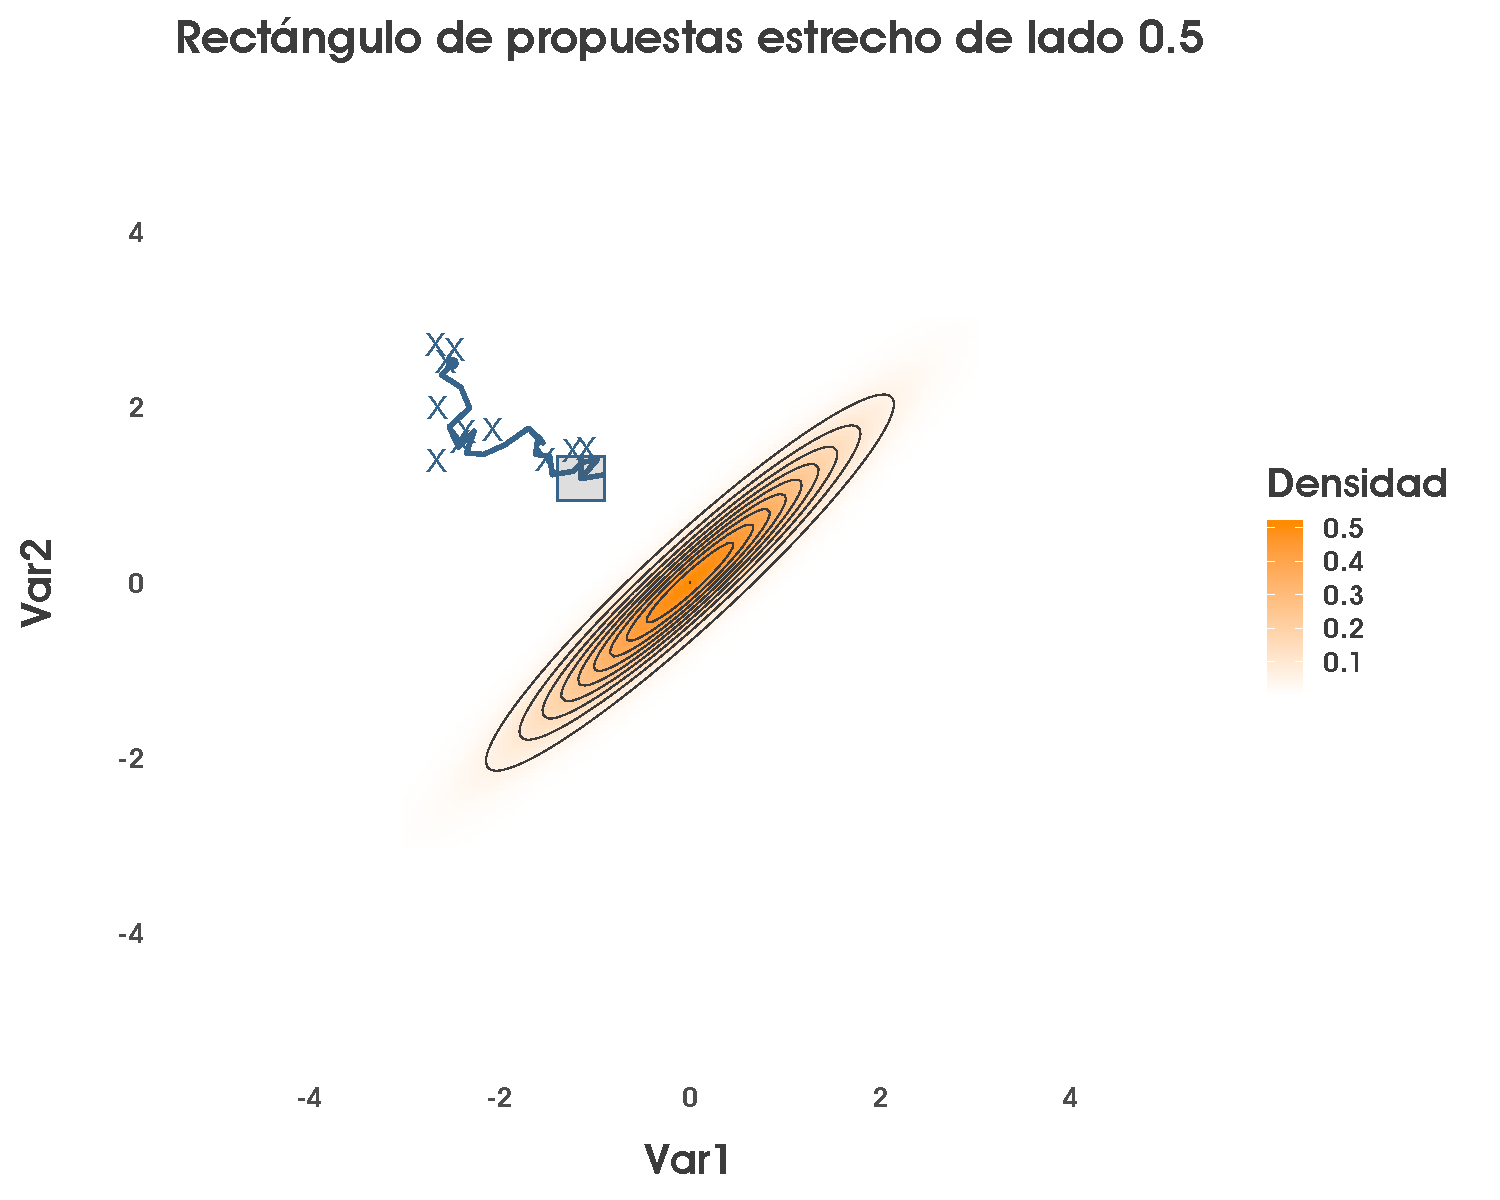
\includegraphics[width=\textwidth]{Figs/Bayes/Ejemplo_RWM_Compara1}
        \caption{Un kernel de propuestas demasiado estrecho acepta más propuestas pero se mueve lento.}
    \end{subfigure}
    ~ 
    \begin{subfigure}{0.3\textwidth}
        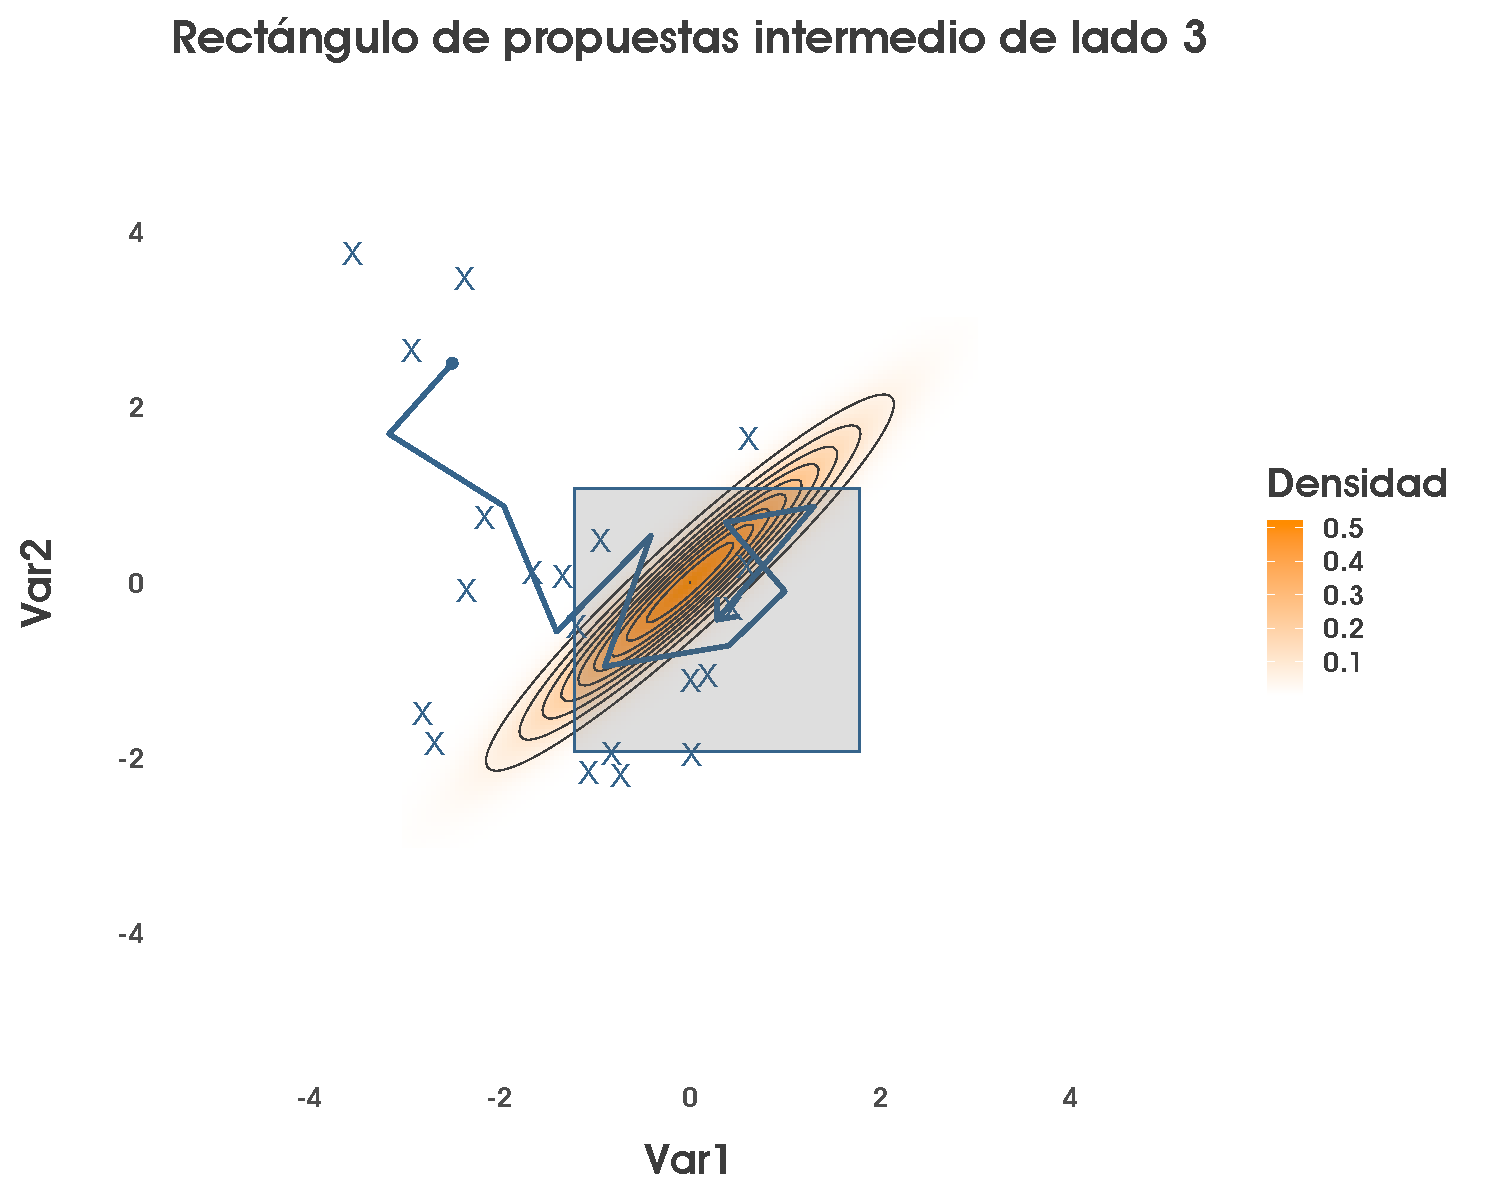
\includegraphics[width=\textwidth]{Figs/Bayes/Ejemplo_RWM_Compara2}
        \caption{El kernel óptimo en general es uno que permita alcanzar regiones diferentes del espacio sin rechazar ``demasiadas'' propuestas. Esto permite que la cadena avance de mejor manera.}
    \end{subfigure}
    ~
    \begin{subfigure}{0.3\textwidth}
        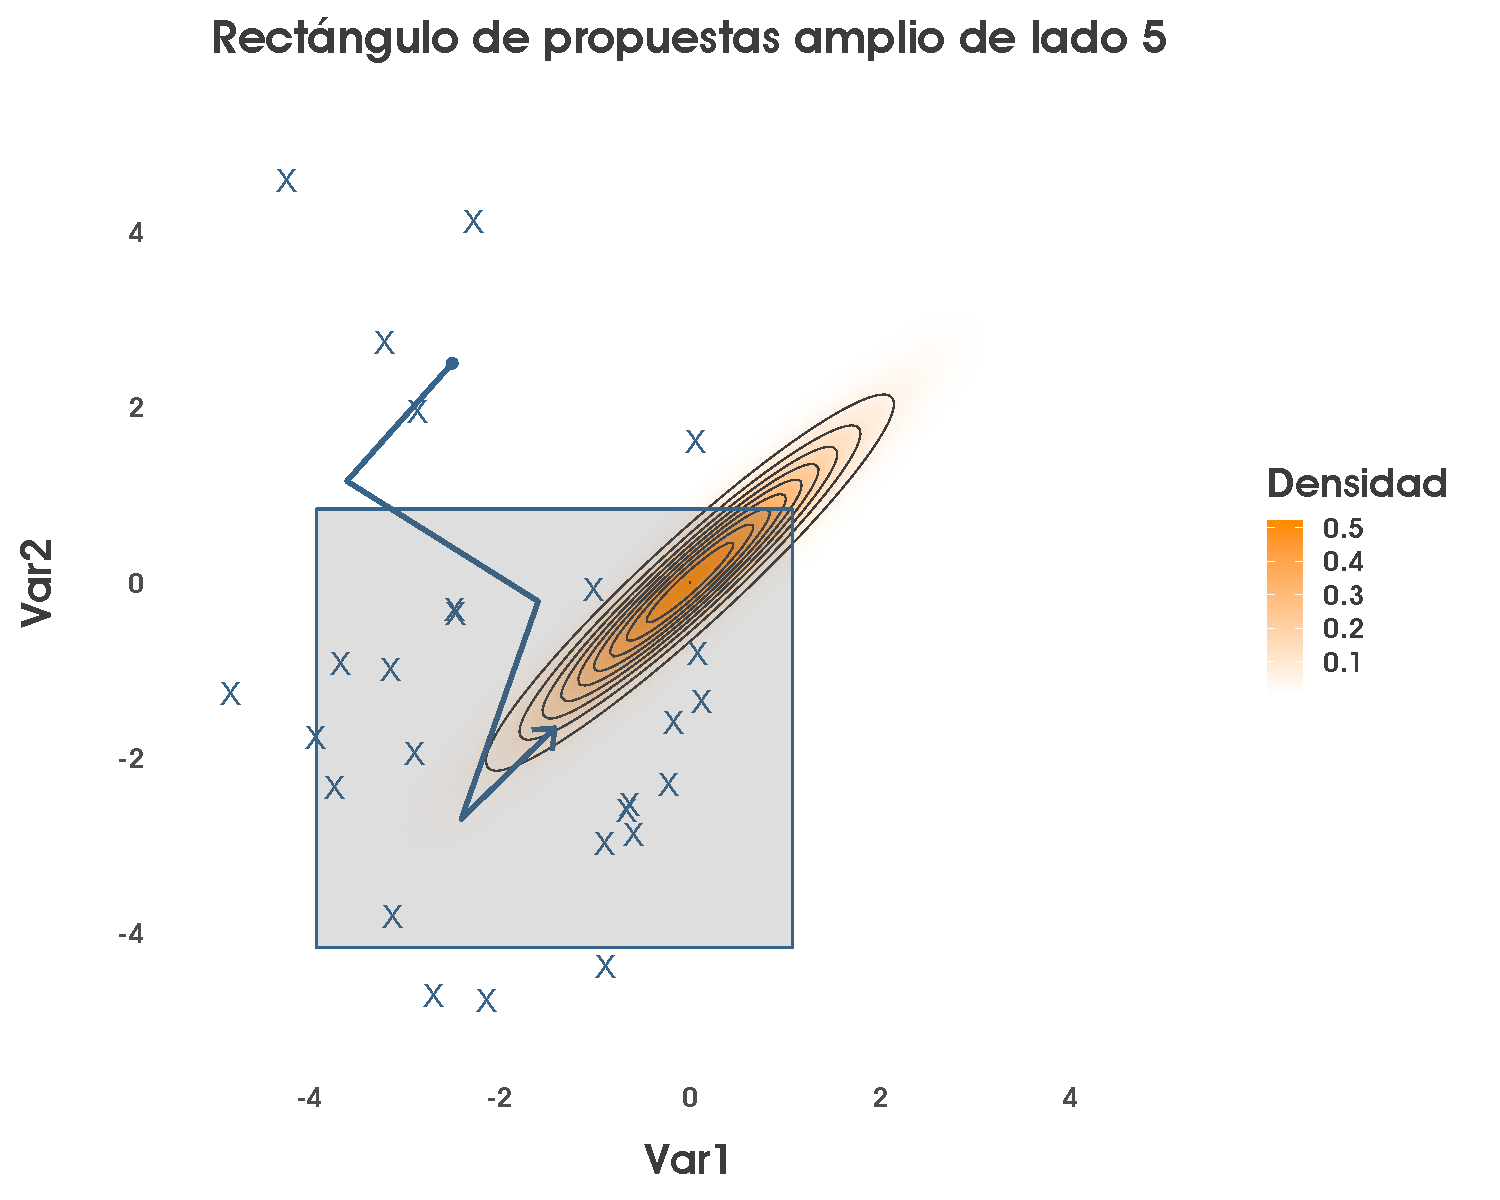
\includegraphics[width=\textwidth]{Figs/Bayes/Ejemplo_RWM_Compara3}
        \caption{Un kernel de propuestas demasiado amplio rechaza demasiadas propuestas. Esto puede provocar que la cadena quede ``atorada'' en el mismo lugar por varias propuestas, lo que a su vez implica un avance más lento.}
    \end{subfigure}
    ~
    \caption{Comparación de kerneles uniformes de propuestas para simular una normal bivariada con correlación $0.95$ mediante RWM. Las tres cadenas presentan las primeras $30$ transiciones, aunque no se repiten los puntos en los que la cadena permanece en el mismo estado. Fuente: elaboración propia.}\label{fig:RWM_Corr}
\end{figure}

Ciertamente hay investigación enfocada a proponer ``reglas de dedo'' que sean relativamente eficientes \parencites{GelmanRobertsGilks96,Geyer05,YangRdz13}. Para el ejemplo original de normales bivariadas no correlacionadas elegí el rectángulo uniforme de lado $3$ porque \textcite{YangRdz13} encuentran que este es el ancho óptimo para simular una normal estándar mediante un kernel uniforme. El uso del kernel uniforme se debe a que es fácil de entender y fue el utilizado por los científicos de Los Álamos, pero pueden haber kérneles más eficientes como reporta el mismo artículo.\\ 

 El problema crece porque la dimensionalidad de los problemas hace que muy rápidamente nos alejemos de los ejemplos triviales y seamos incapaces de proponer kérneles de transición que funcionen de manera adecuada. ¿Qué hacer? Por varios años esto desalentó el uso de los métodos MCMC, hasta la década de los 90 cuando hubo una ``epifanía'' en el mundo de la estadística bayesiana \parencite{RobertCasella11}. 

\subsection{Gibbs Sampler}

\textcite{GelfandSmith90} presentaron un artículo titulado \textit{Sampling-Based Approaches to Calculating Marginal Densities}. En él rescataron tres algoritmos de simulación para obtener densidades que no pueden ser conocidas de manera analítica. Sin embargo, el que provocó la explosión de los métodos bayesianos fue el llamado \textit{Gibbs Sampler}.\\ 

Este algoritmo de MCMC fue propuesto por \textcite{GemanGeman84} mientras trabajaban en problemas de reconstrucción de imágenes, pero ya estaba oculto en el artículo de \textcite{Hastings70} cuando sugería que para simular de una distribución multidimensional se podría cambiar de manera secuencial una única coordenada o, incluso, subgrupos de coordenadas. En otras palabras, ``divide y vencerás''; si el problema es que la distribución objetivo es de alta dimensionalidad y compleja, ¿por qué no intentar simularla por partes más simples en lugar de querer simularla directamente?\\ 

La gran contribución de los hermanos Geman fue encontrar una manera simple y poderosa de llevarlo a cabo. La chispa de Gelfand y Smith fue mostrarle al mundo estadístico que--- sin ser el método más eficiente para cualquier problema--- podía ser bastante eficiente en un amplio rango de problemas comúnmente encontrados en la práctica y, mejor aún, era efectivamente simple y universal \parencite{GelfandEtAl90}.\\

Cuando el vector que queremos simular es bivariado--- digamos $Z = (X,Y)$--- el algoritmo consiste en alternar simulaciones simples de cada variable condicional en la otra, conservando los vectores bivariados de cada ciclo de dos \textit{pasos de Gibbs}. Primero simulamos de $X|Y$, luego de $Y|X$; volvemos a simular otra $X$ dada la $Y$ anterior, luego otra $Y$ dada la nueva $X$ y así sucesivamente. Una analogía imperfecta pero que me funciona como recurso pnemotécnico para recordar el \textit{Gibbs Sampler} es imaginar que mi objetivo es cruzar de algún punto en una acera a otro punto en la acera contraria. En lugar de cruzar la calle de manera diagonal en un solo paso, cruzamos mediante dos. El primero es caminar por la misma banqueta hasta alguna esquina y el segundo es cruzar la calle sobre el paso peatonal. Estos dos pasos constituirían una \textit{transición de Gibss} y repitiendo transiciones de este tipo podríamos caminar de una dirección alejada a algún punto de interés en la ciudad.\\ 

De manera más general, el \textit{Gibbs Sampler} construye una cadena de Markov con base en las llamadas distribuciones \textit{condicionales completas}. Estas no son otra cosa más que las distribuciones condicionales de una o más variables dentro de un vector, dado el resto. Supongamos que tenemos un vector de parámetros $\theta$ de dimensión $d$ expresado mediante una partición $\theta = (\theta_1, \theta_2, \dots, \theta_k)$ donde $\theta_j \in \mathbb{R}^{d_j}$ y $\sum\limits_{j=1}^k d_j = d$. Para cada subvector $\theta_j$, definimos la correspondiente condicional completa como $f(\theta_j|\theta_{-j},y)$, donde $\theta_{-j}$ significa todos los componentes del vector menos el $j$-ésimo. Como estamos en un contexto de aprendizaje bayesiano, las distribuciones son posteriores; es decir, también condicionamos en los datos observados $y$.\\

Una transición de Gibbs se construye, al igual que en el caso bivariado y la analogía, mediante pasos de Gibbs intermedios, como puede verse en el \textbf{Algoritmo \ref{alg:GS}}. Empezando en un vector $\theta^{(0)}$ en el espacio de estados multidimensional, caminamos sobre la banqueta, simulando un valor $\theta_1^{(1)}$ dejando el resto de las variables fijas. Sustituimos este valor en el vector y, ahora, simulamos un valor $\theta_2^{(1)}$ de la correspondiente condicional completa. Así, cada subvector $\theta_j^{(1)}$ se simula con base en los nuevos valores de subvectores que van primero en la secuencia pero con los valores de la transición anterior para los subvectores que sigan en la secuencia. El último paso de la transición será entonces simular $\theta_k^{(1)}$ dados todos los nuevos valores simulados.\\ 

\begin{algorithm}
\DontPrintSemicolon
Valor inicial arbitrario o simulado $\theta^{(0)}\leftarrow (\theta_1^{(0)},\theta_2^{(0)},\dots,\theta_k^{(0)})$\;
\For{$n \leftarrow 1$ \KwTo $N$}{
$\theta_1^{(n)} \sim f(\theta_1|\theta_{-1}^{(n-1)},y)$\;
\For{$j \leftarrow 2$ \KwTo $k-1$}{
	$\theta_j^{(n)} \sim f(\theta_j|\theta_1^{(n)},\dots, \theta_{j-1}^{(n)}, \theta_{j+1}^{(n-1)}, \dots, \theta_k^{(n-1)}, y)$\;
}
$\theta_k^{(n)} \sim f(\theta_k|\theta_{-k}^{(n)},y)$\;
$\theta^{(n)} \leftarrow (\theta_1^{(n)},\theta_2^{(n)},\dots,\theta_k^{(n)})$\;
}

\caption{Gibbs Sampler para el aprendizaje bayesiano \label{alg:GS}}
\end{algorithm}

El algoritmo podría parecer a primera vista poco práctico porque, si no se conoce la distribución conjunta, ¿cómo conoceríamos las $k$ condicionales completas? Sin embargo, como mostraron \textcite{GelfandSmith90} o \textcite{GelfandEtAl90}, es factible aplicarlo a modelos tan variados como multinomiales, normales multivariadas y modelos jerárquicos como regresiones de interceptos y coeficientes variables. La clave está en que las condicionales completas son proporcionales a la posterior pero simplificadas, pues al condicionar solo conservamos los términos que incluyen al respectivo subvector $\theta_j$. Esto permite generalmente identificar una familia de distribuciones conocida o encontrar un algoritmo relativamente sencillo para simular de dicha distribución no normalizada.\\

Quizás la familia de modelos que mejor ejemplifican la utilidad del \textit{Gibbs Sampler} son los modelos jerárquicos. La propia estructura jerárquica implica de manera natural que las condicionales completas se simplifiquen puesto que cada grupo de parámetros es condicionalmente independiente de los otros, dados los hiperparámetros correspondientes. Para verlo podemos seguir el ejemplo de \textcite{GP16}, suponiendo el siguiente modelo jerárquico simple de 3 niveles. Los datos $y$ provienen de $m$ subpoblaciones con el respectivo vector de parámetros $\omega$ que, a su vez, depende de un vector de hiperparámetros $\phi$ con su respectiva hiperinicial: 
\begin{align*}
&f(y|\omega) = \prod\limits_{i=1}^m f(y_i|\omega_i)\\
&f(\omega|\phi) = \prod\limits_{i=1}^m f(\omega_i|\phi)\\
&f(\phi)
\end{align*}

Tenemos en total $m+1$ parámetros $\theta = (\omega, \phi) = (\omega_1,\omega_2,\dots,\omega_m,\phi)$ cuya distribución posterior --- $f(\theta = (\omega, \phi)|y) \propto f(\phi)\prod\limits_{i=1}^m f(y_i|\omega_i)f(\omega_i|\phi)$--- presenta una factorización que simplifica las condicionales completas: 
\begin{align*}
f(\theta_1|\theta_{-1},y) &\propto f(\omega_1|\phi,y_1) \\
\vdots &\\
f(\theta_m|\theta_{-m},y) &\propto f(\omega_m|\phi,y_m) \\
f(\theta_{m+1}|\theta_{-(m+1)},y) &\propto f(\omega|\phi)f(\phi)
\end{align*}

La consagración del \textit{Gibbs Sampler} como la principal herramienta de simulación y aprendizaje práctico bayesiano se dio cuando en la primera mitad de la década de los 90 fue presentado el 	software BUGS, que es un acrónimo para \textit{Bayesian inference Using Gibbs Sampling}. Ya era posible automatizar la aplicación del algoritmo para una clase amplia de modelos que el usuario define mediante distribuciones iniciales, verosimilitudes y datos. Como bien dicen \textcite{CasellaGeorge92}, al liberar a los estadísticos de tener que tratar con cálculos complicados, la atención principal se puede dedicar a los aspectos estadísticos de los problemas. 

\subsection{Convergencia}

La convergencia de los promedios ergódicos que implica \eqref{eq:Teo_Erg_Conv_Prom} es ciertamente importante. Sin embargo, en un análisis bayesiano la única receta indica tener una muestra aleatoria de la distribución posterior. Si observamos con cuidado \eqref{eq:Teo_Erg_Conv_D}, vemos que la última simulación de la cadena es la que podemos considerar como proveniente de la distribución objetivo límite. Si quisiéramos una muestra de tamaño $N$ deberíamos correr $N$ cadenas independientes. Afortunadamente, en las cadenas de MH y MCMC en general, la distribución límite es también lo que se conoce como \textit{distribución estacionaria} de la cadena de Markov. Esto quiere decir que, si se tiene una observación distribuida\\

\section{Hamiltonian Monte Carlo}

%% Parte III %%
\part{Modelado de Datos Franceses}
	
	\chapter{Datos franceses}

Como adelantaba en la introducción, la tercera parte de este trabajo consiste concretamente en el modelado estadístico de los datos franceses que permitan la exploración de las configuraciones sociales que favorecieron o inhibieron el voto por el \textit{Front National} en las elecciones Presidenciales y Legislativas de 2007 y 2012. Por lo mismo, debo comenzar  presentando dichos datos y realizando un análisis exploratorio.

\section{Datos electorales}

En Francia existe una gran variedad de partidos políticos repartidos a lo largo del espectro político, tradicionalmente asociado con las nociones de izquierda y derecha. Adicionalmente, no es raro que los partidos cambien de nombres o formen coaliciones. Las cuatro elecciones consideradas reflejan ambos fenómenos. En 2007 hubo 12 candidaturas presidenciales y 10 en 2012. Para las elecciones legislativas en ambos años se presentaron 17 etiquetas políticas diferentes. Por ello, y para simplificar el análisis, conviene agrupar las diferentes opciones políticas bajo algunas etiquetas generales.\\ 

\begin{table}[H]
\centering
\resizebox{\linewidth}{!}{
\begin{tabular}{l c r r r r}
\multicolumn{6}{c}{\textbf{Elecciones Presidenciales 2007}} \\[5pt] 
\multirow{2}{*}{\textbf{Candidato(a)}} & 
\multirow{2}{*}{\textbf{Partido}} & 
\multicolumn{1}{c}{\textbf{Votos}} & \textbf{\% Ef.} & 
\multicolumn{1}{c}{\textbf{Votos}} & \textbf{\% Ef.}\\ 
& &  
\multicolumn{2}{c}{1ra vuelta} & 
\multicolumn{2}{c}{2da vuelta} \\[2pt] 
\hline
 & & & & & \\[\dimexpr-\normalbaselineskip+3pt]
Nicolas Sarkozy & UMP & 11,448,663 & 31.18 & 18,983,138 & 53.06 \\
Ségolène Royal & PS & 9,500,112 & 25.87 & 16,790,440 & 46.94\\
\hdashline
François Bayrou & UDF & 6,820,119 & 18.57 & & \\
Jean Marie Le Pen & FN & 3,834,530 & 10.44 & & \\
Olivier Besancenot & LRO & 1,498,581 & 4.08 & & \\
Philippe de Villiers & MPF & 818,407 & 2.23 & & \\
Marie-George Buffet & PC & 707,268 & 1.93 & & \\
Dominique Voynet & Verts & 576,666 & 1.57 & & \\
Arlette Laguiller & LO & 487,857 & 1.33 & & \\
José Bové & Indep. & 483,008 & 1.32 & & \\
Frédérick Nihous & CPNT & 420,645 & 1.15 & & \\
Gérard Schivardi & PT & 123,540 & 0.34 & & \\[3pt]
\hline
 & & & & & \\[\dimexpr-\normalbaselineskip+3pt]
\multicolumn{2}{l}{\textbf{Votación efectiva}} 
& 36,719,396 &
& 35,773,578 & \\
\multicolumn{2}{l}{Blancos o nulos} 
& 534,846 & 
& 1,568,426 & \\[3pt]
\hline
 & & & & & \\[\dimexpr-\normalbaselineskip+3pt]
\multicolumn{2}{l}{\textbf{Votación emitida}} 
& 37,254,242 & 
& 37,342,004 & \\
\multicolumn{2}{l}{Abstenciones} 
& 7,218,592 & 
& 7,130,729 & \\[3pt]
\hline
 & & & & & \\[\dimexpr-\normalbaselineskip+3pt]
\multicolumn{2}{l}{\textbf{Lista nominal}} 
& 44,472,834 & 
& 44,472,733 & \\
\end{tabular}
}
\caption{Resultados de las elecciones presidenciales francesas de 2007, resultando presidente electo Nicolas Sarkozy (UMP). Fuente: elaboración propia con los datos oficiales del Ministerio del Interior.}
\label{tbl:Resul_Oficiales_P07}
\end{table}

\begin{sidewaystable}[ph!]
\centering
\resizebox{\linewidth}{!}{
\begin{tabular}{l c r r c r r c c}
\multicolumn{9}{c}{\textbf{Elecciones Legislativas 2007}} \\[5pt] 
\multicolumn{2}{c}{\multirow{2}{*}{\textbf{Plataforma política}}} & 
\textbf{Votos} & 
\textbf{\% Ef.} & 
\textbf{Asientos} &
\textbf{Votos} & 
\textbf{\% Ef.} & 
\textbf{Asientos} &
\multirow{2}{*}{\textbf{Total de Asientos}}\\ 
\multicolumn{2}{c}{} 
& \multicolumn{3}{c}{1ra vuelta} 
& \multicolumn{3}{c}{2da vuelta} 
& \\[2pt] 
\hline
 & & & & & & & &\\[\dimexpr-\normalbaselineskip+3pt]
Union pour un Mouvement Populaire & UMP 
& 10,289,737 & 39.54 & 98 & 9,460,710 & 46.36 & 215 & 313 \\
Socialiste & SOC 
& 6,436,520 & 24.73 & 1 & 8,624,861 & 42.27 & 185 & 186 \\
Majorité Présidentielle & MAJ
& 616,440 & 2.37 & 8 & 433,057 & 2.12 & 14 & 22\\
Parti Communiste Français & COM 
& 1,115,663 & 4.29 & - & 464,739 & 2.28 & 15 & 15\\
Divers Gauche & DVG
& 513,407 & 1.97 & - & 503,556 & 2.47 & 15 & 15\\
Divers Droite & DVD 
& 641,842 & 2.47 & 2 & 238,588 & 1.17 & 7 & 9\\
Radicales de Gauche & RDG
& 343,565 & 1.32 & - & 333,194 & 1.63 & 7 & 7\\
Les Verts & VEC
& 845,977 & 3.25 & - & 90,975 & 0.45 & 4 & 4\\
Union pour la Démocratie Française & UDFD 
& 1,981,107 & 7.61 & - & 100,115 & 0.49 & 3 & 3\\
Mouvement pour la France & MPF
& 312,581 & 1.20 & 1 & - & - & - & 1\\
Divers & DIV 
& 267,760 & 1.03 & - & 33,068 & 0.16 & 1 & 1\\
Régionaliste & REG
& 133,473 & 0.51 & - & 106,484 & 0.52 & 1 & 1\\
Front National & FN 
& 1,116,136 & 4.29 & - & 17,107 & 0.08 & - & -\\
Extrême Gauche & EXG 
& 888,250 & 3.41 & - & -  & - & - & -\\
Chase Pêche Nature Traditions & CPNT 
& 213,427 & 0.82 & - & - & - & - & -\\
Ecologistes & ECO 
& 208,456 & 0.80 & - & - & - & - & -\\
Extrême Droite & EXD 
& 102,124 & 0.39 & - & - & - & - & -\\[3pt]
\hline
 & & & & & & & & \\[\dimexpr-\normalbaselineskip+3pt]
\multicolumn{2}{l}{\textbf{Votación efectiva}} 
& 26,026,465 & &
& 20,406,454 & & & \\
\multicolumn{2}{l}{Blancos o nulos} 
& 495,357 & &
& 722,585 & & & \\[3pt]
\hline
 & & & & & & & &\\[\dimexpr-\normalbaselineskip+3pt]
\multicolumn{2}{l}{\textbf{Votación emitida}} 
& 26,521,822 & &
& 21,129,039 & & & \\
\multicolumn{2}{l}{Abstenciones} 
& 17,374,011 & &
& 14,096,209 & & & \\[3pt]
\hline
 & & & & & & &\\[\dimexpr-\normalbaselineskip+3pt]
\multicolumn{2}{l}{\textbf{Lista nominal}} 
& 43,895,833 & &
& 35,225,248 & & & \\
\end{tabular}
}
\caption{Resultados de las elecciones legislativas de 2007 para el conjunto de todo el territorio francés, incluyendo el ultramar. Fuente: elaboración propia con los datos oficiales del Ministerio del Interior.}
\label{tbl:Resul_Oficiales_L07}
\end{sidewaystable}

\begin{table}[H]
\centering
\resizebox{\linewidth}{!}{
\begin{tabular}{l c r r r r}
\multicolumn{6}{c}{\textbf{Elecciones Presidenciales 2012}} \\[5pt] 
\multirow{2}{*}{\textbf{Candidato(a)}} & 
\multirow{2}{*}{\textbf{Partido}} & 
\multicolumn{1}{c}{\textbf{Votos}} & \textbf{\% Ef.} & 
\multicolumn{1}{c}{\textbf{Votos}} & \textbf{\% Ef.}\\ 
& &  
\multicolumn{2}{c}{1ra vuelta} & 
\multicolumn{2}{c}{2da vuelta} \\[2pt] 
\hline
 & & & & & \\[\dimexpr-\normalbaselineskip+3pt]
François Hollande & PS & 10,272,705 & 28.63 & 18,000,668 & 51.64\\
Nicolas Sarkozy & UMP & 9,753,629 & 27.18 & 16,860,685 & 48.36 \\
\hdashline
Marine Le Pen & FN & 6,421,426 & 17.90 & & \\
Jean-Luc Mélenchon & FG & 3,984,822 & 11.10 & & \\
François Bayrou & MoDem & 3,275,122 & 9.13 & & \\
Eva Joly & EELV & 828,345 & 2.31 & & \\
Nicolas Dupont-Aignan & DLR & 643,907 & 1.79 & & \\
Philippe Poutou & NPA & 411,160 & 1.15 & & \\
Nathalie Arthaud & LO & 202,548 & 0.56 & & \\
Jacques Cheminade & SP & 89,545 & 0.25 & & \\[3pt]
\hline
 & & & & & \\[\dimexpr-\normalbaselineskip+3pt]
\multicolumn{2}{l}{\textbf{Votación efectiva}} 
& 35,883,209 &
& 34,861,353 & \\
\multicolumn{2}{l}{Blancos o nulos} 
& 701,190 & 
& 2,154,956 & \\[3pt]
\hline
 & & & & & \\[\dimexpr-\normalbaselineskip+3pt]
\multicolumn{2}{l}{\textbf{Votación emitida}} 
& 36,584,399 & 
& 37,016,309 & \\
\multicolumn{2}{l}{Abstenciones} 
& 9,444,143 & 
& 9,049,998 & \\[3pt]
\hline
 & & & & & \\[\dimexpr-\normalbaselineskip+3pt]
\multicolumn{2}{l}{\textbf{Lista nominal}} 
& 46,028,542 & 
& 46,066,307 & \\
\end{tabular}
}
\caption{Resultados de las elecciones presidenciales francesas de 2012, resultando presidente electo François Hollande (PS). Fuente: elaboración propia con los datos oficiales del Ministerio del Interior.}
\label{tbl:Resul_Oficiales_P12}
\end{table}

\begin{sidewaystable}[ph!]
\centering
\resizebox{\linewidth}{!}{
\begin{tabular}{l c r r c r r c c}
\multicolumn{9}{c}{\textbf{Elecciones Legislativas 2012}} \\[5pt] 
\multicolumn{2}{c}{\multirow{2}{*}{\textbf{Plataforma política}}} & 
\textbf{Votos} & 
\textbf{\% Ef.} & 
\textbf{Asientos} &
\textbf{Votos} & 
\textbf{\% Ef.} & 
\textbf{Asientos} &
\multirow{2}{*}{\textbf{Total de Asientos}}\\ 
\multicolumn{2}{c}{} 
& \multicolumn{3}{c}{1ra vuelta} 
& \multicolumn{3}{c}{2da vuelta} 
& \\[2pt] 
\hline
 & & & & & & & &\\[\dimexpr-\normalbaselineskip+3pt]
Socialiste & SOC 
& 7,618,326 & 29.35 & 22 & 9,420,889 & 40.91 & 258 & 280 \\
Union pour un Mouvement Populaire & UMP 
& 7,037,268 & 27.12 & 9 & 8,740,628 & 37.95 & 185 & 194 \\
Divers Gauche & DVG
& 881,555 & 3.40 & 1 & 709,395 & 3.08 & 21 & 22\\
Europe-Écologie-Les Verts & VEC
& 1,418,264 & 5.46 & 1 & 829,036 & 3.60 & 16 & 17\\
Divers Droite & DVD 
& 910,034 & 3.51 & 1 & 417,940 & 1.81 & 14 & 15\\
Nouveau Centre & NCE
& 569,897 & 2.20 & 1 & 568,319 & 2.47 & 11 & 12\\
Radicales de Gauche & RDG
& 428,898 & 1.65 & 1 & 538,331 & 2.34 & 11 & 12\\
Front de Gauche & FG 
& 1,793,192 & 6.91 & - & 249,498 & 1.08 & 10 & 10\\
Parti Radical & PRV
& 321,124 & 1.24 & - & 311,199 & 1.35 & 6 & 6\\
Front National & FN 
& 3,528,663 & 13.60 & - & 842,695 & 3.66 & 2 & 2\\
Le Centre pour la France & CEN
& 458,098 & 1.77 & 1 & 113,196 & 0.49 & 2 & 2\\
Alliance Centriste & ALLI 
& 156,026 & 0.60 & - & 123,132 & 0.53 & 2 & 2\\
Régionaliste & REG
& 145,809 & 0.56 & - & 135,312 & 0.59 & 2 & 2\\
Extrême Droite & EXD 
& 49,499 & 0.19 & - & 29,738 & 0.13 & 1 & 1\\
Extrême Gauche & EXG 
& 253,386 & 0.98 & - & - & - & - & -\\
Ecologistes & ECO 
& 249,068 & 0.96 & - & - & - & - & -\\
Autres & AUT 
& 133,752 & 0.52 & - & - & - & - & -\\[3pt]
\hline
 & & & & & & & & \\[\dimexpr-\normalbaselineskip+3pt]
\multicolumn{2}{l}{\textbf{Votación efectiva}} 
& 25,952,859 & &
& 23,029,308 & & & \\
\multicolumn{2}{l}{Blancos o nulos} 
& 416,267 & &
& 923,178 & & & \\[3pt]
\hline
 & & & & & & & &\\[\dimexpr-\normalbaselineskip+3pt]
\multicolumn{2}{l}{\textbf{Votación emitida}} 
& 26,369,126 & &
& 23,952,486 & & & \\
\multicolumn{2}{l}{Abstenciones} 
& 19,712,978 & &
& 19,281,162 & & & \\[3pt]
\hline
 & & & & & & &\\[\dimexpr-\normalbaselineskip+3pt]
\multicolumn{2}{l}{\textbf{Lista nominal}} 
& 46,082,104 & &
& 43,233,648 & & & \\
\end{tabular}
}
\caption{Resultados de las elecciones legislativas de 2012 para el conjunto de todo el territorio francés, incluyendo el ultramar. Fuente: elaboración propia con los datos oficiales del Ministerio del Interior.}
\label{tbl:Resul_Oficiales_L12}
\end{sidewaystable}

Dependiendo de la posición--- aproximada--- de la plataforma política en el eje ideológico izquierda-derecha es posible clasificar a la mayoría de las opciones en los siguientes grupos. En primer lugar, debido al interés específico en el Front National, este es clasificado individualmente. Posteriormente, tenemos a los partidos tradicionales de derecha e izquierda--- el UMP\footnote{Hoy en día este partido cambió de nombre y ahora se conoce como \textit{Les Republicains}. En 2007, después de que Nicolas Sarkozy ganara las elecciones, además de los candidatos del UMP hubo candidaturas bajo la etiqueta de la \textit{Mayoría presidencial} por lo que también las agrupo junto con el UMP.} y los socialistas del PS, respectivamente---. Además, existen plataformas de centro, así como otras izquierdas y derechas. Finalmente, existen opciones con un fuerte componente temático--- como los verdes o los regionalistas--- o con una plataforma política especial de forma tal que resulta más conveniente separarlos del eje y clasificarlos en una categoría residual. Así pues, en total existen 7 grupos generales: 

\begin{itemize}
\item FN
\item Derecha
\item Izquierda
\item Centro
\item Otras derechas
\item Otras izquierdas
\item Otros
\end{itemize}

En la \textbf{Figura \ref{fig:Partidos_07_12}} pueden observarse representaciones esquemáticas de esta simplificación del espectro político francés para 2007 y 2012.\\

\begin{figure}[h]
	\centering
	\begin{subfigure}{0.9\textwidth}
	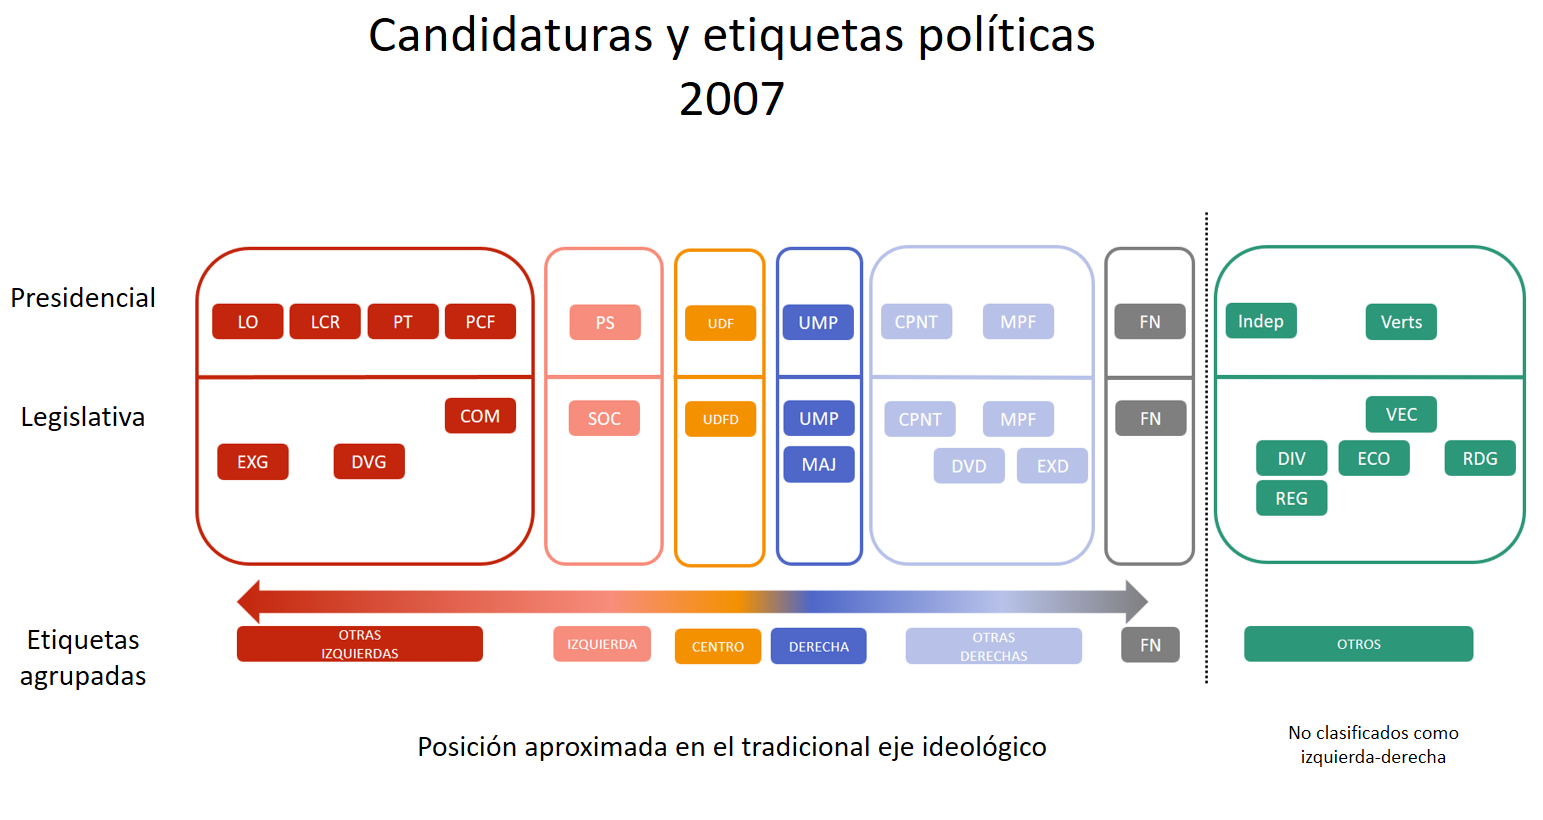
\includegraphics[width = \textwidth]{Figs/FN_Francia/Partidos_07}
	\end{subfigure}	
	~
	\begin{subfigure}{0.9\textwidth}
	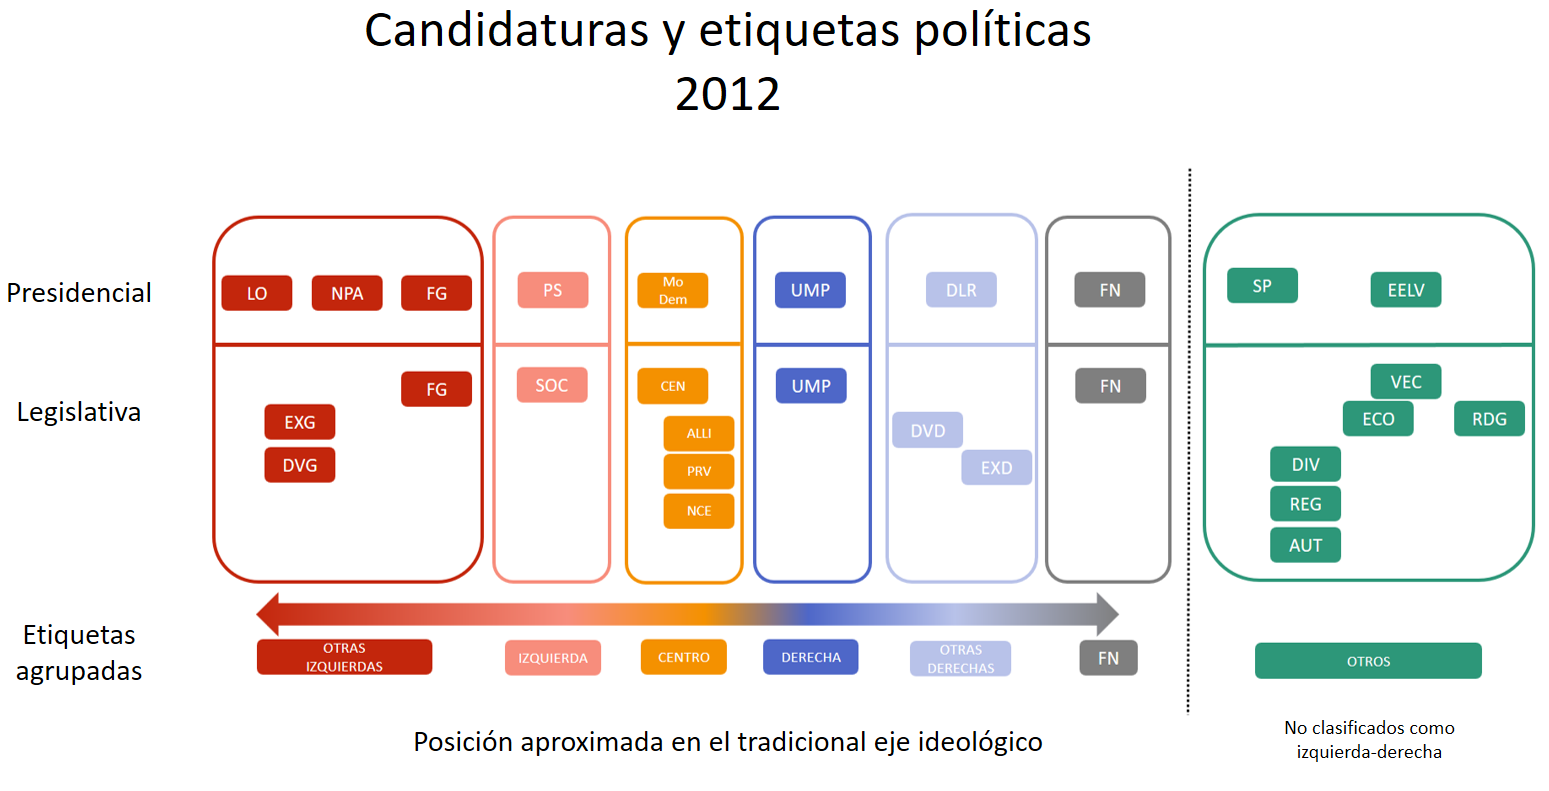
\includegraphics[width = \textwidth]{Figs/FN_Francia/Partidos_12}
	\end{subfigure}		
	\caption{Representación esquemática de los partidos, candidaturas y etiquetas políticas en las elecciones francesas de 2007 y 2012. Fuente: elaboración propia.}
	\label{fig:Partidos_07_12}	
\end{figure}

En las elecciones de 2007 la derecha tradicional fue la ganadora pues Nicolas Sarkozy obtuvo la presidencia y consiguieron 313 escaños en la Asamblea Nacional bajo la etiqueta UMP y 22 más bajo la etiqueta de Mayoría Presidencial. En 2012, sin embargo, Sarkozy perdió la reelección frente al socialista François Hollande y la izquierda tomó el control del Hemiciclo con 280 diputados.\\ 

Por su parte, Jean-Marie Le Pen como candidato presidencial frontista en 2007 obtuvo 10.44\% de la votación efectiva en la primera vuelta, quedando en cuarta posición y fuera de la segunda vuelta. Más aún, el FN no logró conseguir ningún diputado a pesar de obtener más de 1 millón de votos en las primeras vueltas. Cinco años después, ya con Marine Le Pen como lideresa y candidata presidencial, el partido obtuvo 17.90\% de la votación efectiva en la primera vuelta. Ese porcentaje representó el 3er lugar en la elección, insuficiente de nueva cuenta para disputar la segunda vuelta electoral. En las elecciones legislativas, sin embargo, el partido sí tuvo un crecimiento, logrando alrededor de 3 millones y medio de sufragios en la primera vuelta--- equivalentes al 13.60\%---. En la segunda vuelta el FN consiguió 2 diputaciones.\\ 

Estos resultados y algunos otros pueden consultarse en el {\color{Red} Anexo B}.
	%\chapter{Modelado}

En este capítulo desarrollo el proceso de modelado de los datos franceses con tal de explorar las configuraciones sociales que favorecieron o inhibieron el voto por el FN en 2012. Para ello hay que notar que los datos electorales que considero son el número de votos por Marine Le Pen en cada comuna así como el número de inscritos en el listado nominal de las mismas. Tenemos entonces $C$ pares de la forma $\left\lbrace y_c, n_c \right\rbrace$ donde $y_c$ representa el número de votos y $n_c$ el de inscritos en la comuna $c$. Este tipo de datos puede ser modelado como proveniente de una distribución binomial con número de ensayos conocido y parámetro de interés $p_c$: 

\begin{equation*}
y_c|p_c \sim Binom(n_c, p_c) \quad \forall \; c \, \in \mathbb{N}_C
\end{equation*} 

Podemos interpretar cada parámetro $p_c$ como la afinidad que se tuvo en la comuna $c$ por Marine Le Pen en la primera vuelta presidencial de 2012. Esta afinidad es la que quisiéramos explicar en términos de configuraciones sociales.\\

Recordando la presentación de la regresión logística en la \textbf{\autoref{Sec:Pres_Logis}}, si tenemos un vector $x_c$ de variables explicativas en la comuna $c$, construimos un MLG de la siguiente manera: 

\begin{align*}
y_c|\theta & \sim Binom(n_c,p_c) \quad \forall \quad c \in \mathbb{N}_C \\
\text{con} \quad ln\left(\dfrac{p_c}{1-p_c}\right) &= \alpha + \beta x_c \nonumber \\
\text{y} \quad \theta &= (\alpha,\beta) \sim f(\theta)
\end{align*}

En nuestro caso, sin pérdida de generalidad, para la $m$-ésima variable explicativa tenemos un vector de proporciones $x_c=(x_{1,c},\dots,x_{l_m,c})$ donde $l_m$ es el número de categorías de la variable y $x_{j,c}=1 - \sum_{k\neq j} x_{k,c}$ para toda $j \in \mathbb{N}_{l_m}$. Recordando el problema de multicolinealidad que esto ocasionaría al considerar la regresión con intercepto--- \autoref{prob_multicolinealidad}--- podemos definir una restricción de identificabilidad de suma cero para los coeficientes, de manera tal que $\beta_j=-\sum\limits_{k\neq j}\beta_k$.\\

Para ilustrarlo, si tomáramos como variable explicativa la composición por edad de la población comunal, tendríamos $x_c=(Ed1_c, \dots, Ed6_c)$ donde $Edj_c$ es la proporción de habitantes del grupo de edad $j$. En este caso, $\beta_{6} = -\sum\limits_{k = 1}^5 \beta_k$, por lo que en realidad solo tenemos libres el intercepto y 5 coeficientes a la hora de asignar la distribución inicial $f(\theta)$. 

\begin{align*}
y_c|\theta & \sim Binom(n_c,p_c) \quad \forall \quad c \in \mathbb{N}_C \\
\text{con} \quad ln\left(\dfrac{p_c}{1-p_c}\right) &= \alpha + \beta_1Ed1_c + \dots + \beta_6Ed6_c \quad \text{tal que} \quad \beta_6 = -\sum\limits_{k = 1}^5 \beta_k \nonumber \\
\text{y} \quad \theta &= (\alpha,\beta_1,\dots,\beta_5) \sim f(\theta) 
\end{align*}

\section{Distribuciones inciales}

¿Cómo asignamos distribuciones iniciales? Primero hay que tomar en cuenta que las distribuciones normalmente consideradas como mínimo informativas tienen implicaciones particulares en el contexto de la escala logística. Supongamos que quisiéramos asignar una distribución inicial al valor del predictor lineal $\eta = \alpha + \beta X$. Una distribución $N(\mu=0,\sigma^2=100)$ sería normalmente considerada como una distribución mínimo informativa. Tendría una desviación estándar de $10$, por lo que poco más del 95\% de sus observaciones oscilrían entre $-20$ y $20$. ¿Qué implicación tiene esto para una proporción $p$ vinculada con $\eta$ mediante la liga logística? Es decir, si asignamos esa distribución inicial a $\eta=ln\left(\dfrac{p}{1-p}\right)$, ¿qué estamos diciendo sobre $p$? Podemos observarlo en el primer histograma de la \textbf{Figura \ref{fig:Malas_Iniciales}}. Simulando observaciones de $\eta\sim N(\mu=0,\sigma_1=10)$ vemos que la mayoría de ellas llevan a valores extremos de $p$ cercanos a 0 o a 1. Incluso repitiendo el ejercicio para desviaciones estándar menores como $\sigma_2=5$ o $\sigma_3=2.5$, la distribución inicial lleva a un histograma para $p$ en forma de U. Tendríamos que tener desviaciones estándar más pequeñas, como $\sigma_4=1.5$, o una normal estándar con $\sigma_5=1$ para estar asignando una distribución poco informativa para $p$.\\ 

\begin{figure}[h]
	\centering
	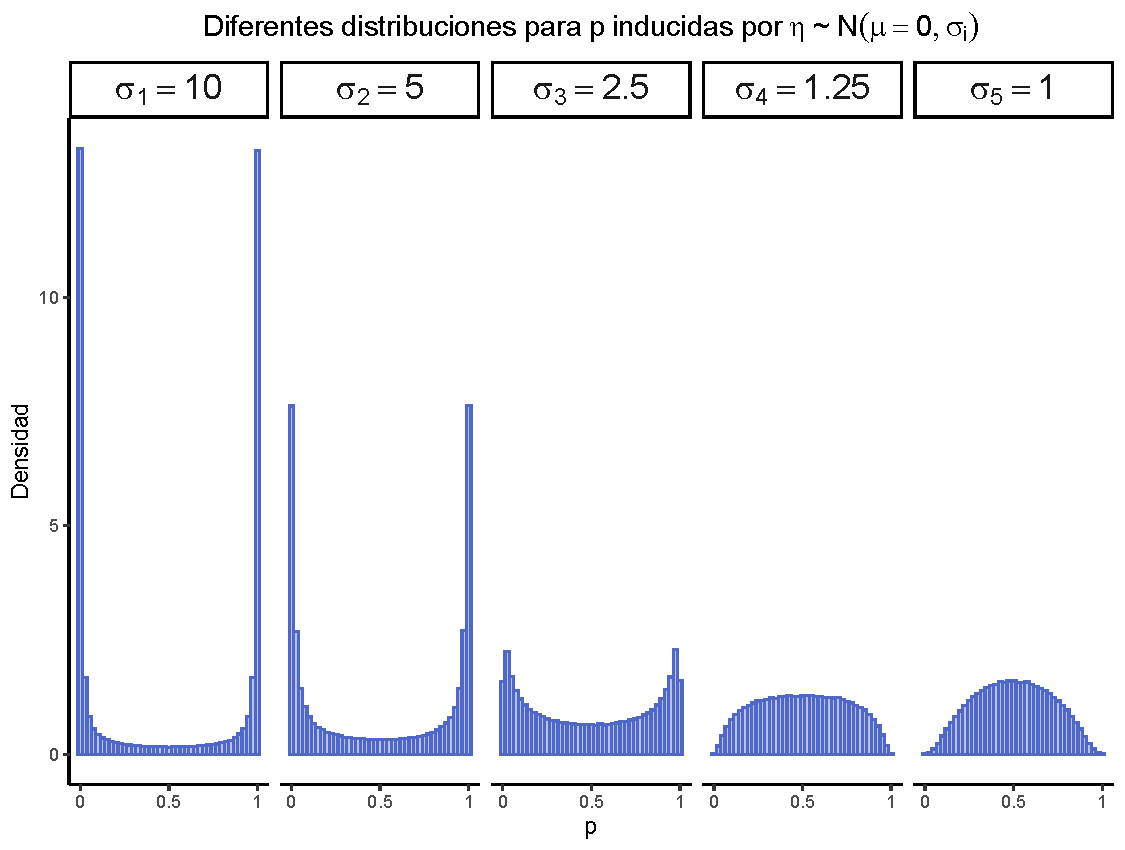
\includegraphics[width = 0.9\textwidth]{Figs/Modelado/Malas_Iniciales}
	\caption{Ejemplo de implicaciones en $p$ con distribuciones iniciales para un predictor lineal. Todas son normales centradas en $0$ con distintos parámetros $\sigma$ de desviación estándar. Fuente: elaboración propia.}
	\label{fig:Malas_Iniciales}
\end{figure}

El motivo es que la función logística no es lineal y tiene que ``compactar'' valores en los reales dentro del espacio confinado del $\left(0,1\right)$. Por decirlo de una manera informal, el verdadero rango de variación de la escala logística son valores de $\eta$ en $(-5,5)$; valores fuera de este intervalo llevan prácticamente a los mismos valores extremos cercanos a 0 o a 1, como apreciamos en la \textbf{Figura \ref{fig:Escala_Logis}}.\\

\begin{figure}[h]
	\centering
	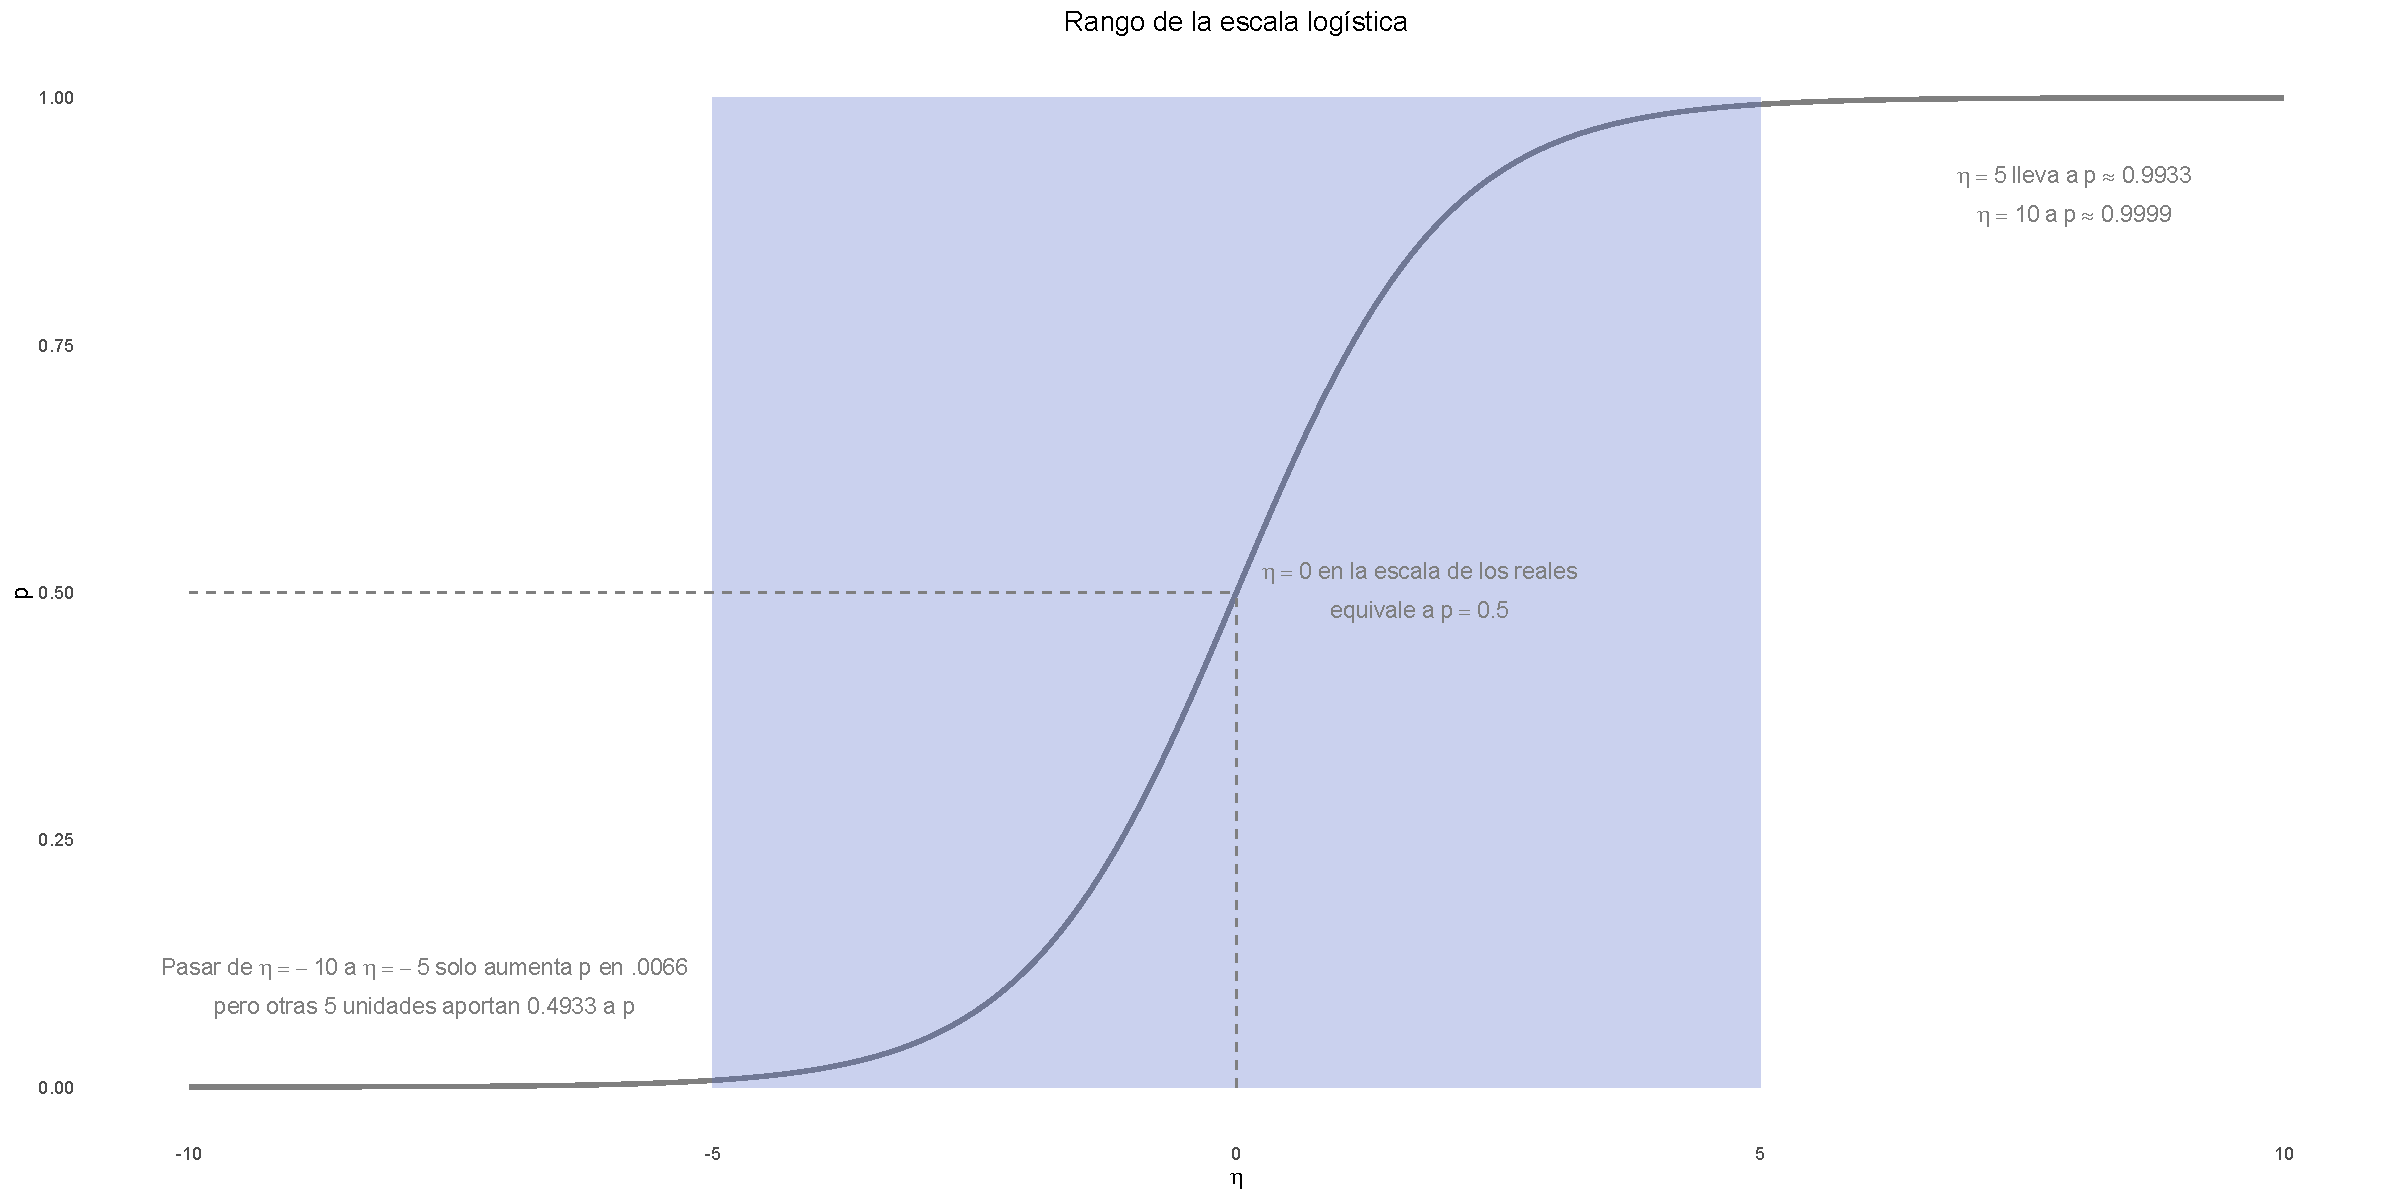
\includegraphics[width = 0.8\textwidth]{Figs/Modelado/Escala_Logis}
	\caption{Fuente: elaboración propia.}
	\label{fig:Escala_Logis}
\end{figure}

Ahora bien, nosotros no asignaremos distribuciones iniciales para el predictor lineal en su conjunto, sino para los coeficientes $\beta$ de dicho predictor lineal. Optaré aquí por una posición un poco escéptica o conservadora. A pesar de lo que sugerían las tendencias ingenuas del capítulo anterior, \textit{a priori}, no buscaría asignarle un sentido al efecto. Asimismo, los efectos de variables ecológicas o agregadas, no deberían ser tan grandes. No querría ``inflar'' la magnitud del valor explicativo mediante la distribución inicial pero tampoco negar la posibilidad de que existan algunos efectos importantes. Considero que una inicial para el coeficiente $\beta\sim N(\mu=0,\sigma=0.5)$ cumple relativamente bien con estas condiciones. Si tomamos el $0$ como referencia y comparamos el valor correspondiente de $p$ con aquel para una $\beta$ una desviación estándar mayor--- i.e. $\beta = 0.5$--- el efecto $\Delta$ sería de aproximadamente $+12$ puntos porcentuales. Si ahora disminuimos $\beta$ en 2 desviaciones estándar,  $\Delta \approx -23$ pp, como puede apreciarse en la \textbf{Figura \ref{fig:Inicial_Coef}}. Sin exagerar su interpretación, pues hay que multiplicar por el valor de la variable explicativa, estos podrían pensarse como los máximos efectos creíbles \textit{a priori}. 

\begin{figure}[h]
	\centering
	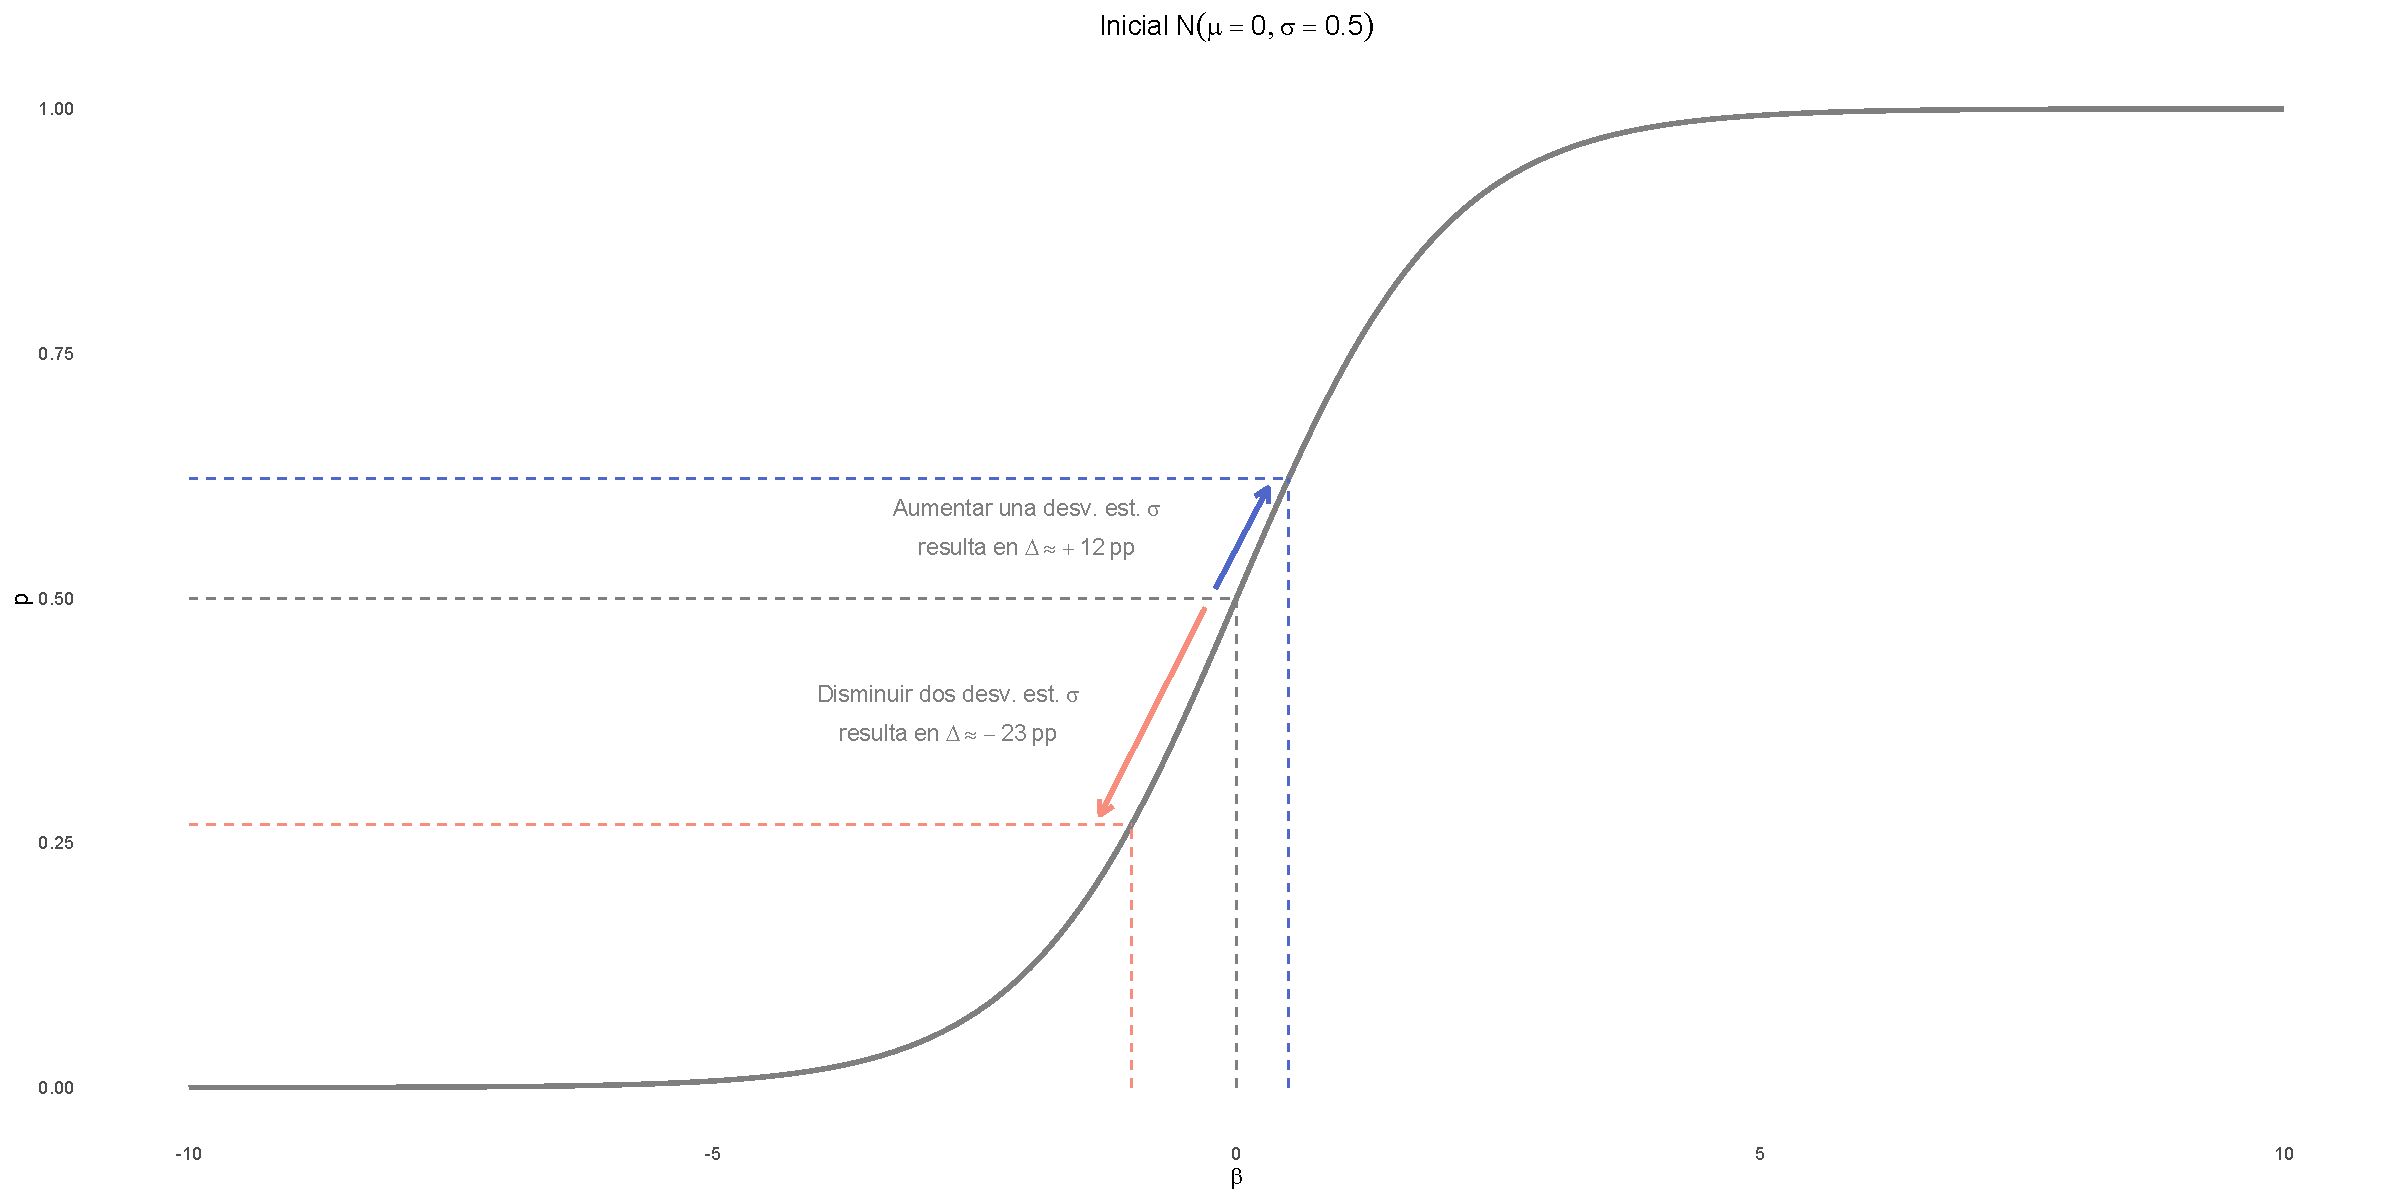
\includegraphics[width = 0.8\textwidth]{Figs/Modelado/Inicial_N0_un_medio}
	\caption{Fuente: elaboración propia.}
	\label{fig:Inicial_Coef}
\end{figure}

Por otro lado, debemos detenernos a pensar en la interpretación del intercepto $\alpha$. Por un lado, $\alpha$ es el valor que tomaría el predictor lineal $\eta_c$, si todos los coeficientes fueran iguales a $0$. Esto nos podría hacer pensar que querríamos que \textit{a priori} su distribución nos lleve a valores cercanos al  17.9\%, porcentaje que obtuvo Le Pen en la elección. Sin embargo, también hay que notar que con variables explicativas de configuraciones sociales, $x_c$, $\alpha$ es el valor que tomaría $\eta_c$ si la población estuviera repartida equitativamente entre todas las categorías. En efecto, supongamos que para la $m$-ésima variable con $l_m$ categorías cada $x_{j,c}=l_m^{-1}$. Tendríamos que

\begin{align*}
\eta_c &= \alpha + \sum\limits_{j=1}^{l_m} \beta_j x_{j,c} = \alpha + \sum\limits_{j=1}^{l_m} \dfrac{\beta_j}{l_m} = \alpha + \dfrac{1}{l_m}\sum\limits_{j=1}^{l_m} \beta_j
\intertext{y por la restricción de identificabilidad de suma cero de los coeficientes,}
&= \alpha + \dfrac{1}{l_m}\left(0\right) = \alpha 
\end{align*}

Tomando en cuenta las teorías del conflicto discutidas en la revisión de literatura, podríamos pensar que si en lugar de tener grupos mayoritarios frente a grupos minoritarios hubiese una sociedad más ``equilibrada'', el voto frontista disminuiría. Así pues, deberíamos buscar una distribución inicial con una media menor al 17.9\% obtenido en las elecciones. También, considerando que puede ser más robusto dilucidar una distribución inicial con base en cuantiles, más que igualar la media podríamos intentar aproximar el rango intercuartílico observado de entre 13.54\% y 21.44\%, pero sesgado un poco a la baja para tomar en cuenta la hipótesis anterior sobre una población equilibrada. Después de algunas pruebas elegí una distribución inicial para $\alpha\sim N(\mu = -1.7,\sigma = 0.25)$.\\

Consideremos ahora una ``comuna promedio'', definida como aquella que tuviera valores promedio en las variables explicativas; podemos realizar simulaciones de la distribución predictiva con estas iniciales. Es decir, simulamos de $\alpha\sim N(\mu = -1.7,\sigma = 0.25)$ y para cada $\beta\sim N(\mu = 0,\sigma = 0.5)$. Calculamos el predictor lineal con base en los valores promedio de cada categoría--- considerando también la restricción de suma cero de los coeficientes--- y tomamos el logit inverso. Este proceso, por ejemplo para grupos de edad, nos lleva al histograma de la \textbf{Figura \ref{fig:Predictiva_Inicial}}, con el modelo

\begin{align*}
y_c|\theta=(\alpha,\beta) & \sim Binom(n_c,p_c) \quad \forall \quad c \in \mathbb{N}_C \\
\text{con} \quad ln\left(\dfrac{p_c}{1-p_c}\right) &= \alpha + \beta_1Ed1_c + \dots + \beta_6Ed6_c \quad \text{tal que} \quad \beta_6 = -\sum\limits_{k = 1}^5 \beta_k \nonumber \\
\text{y} \quad \alpha & \sim N(\mu = -1.7,\sigma = 0.25)\\
\beta_j & \sim N(\mu = 0,\sigma = 0.5) \quad \, j =1,\dots,5
\end{align*}

\begin{figure}[h]
	\centering
	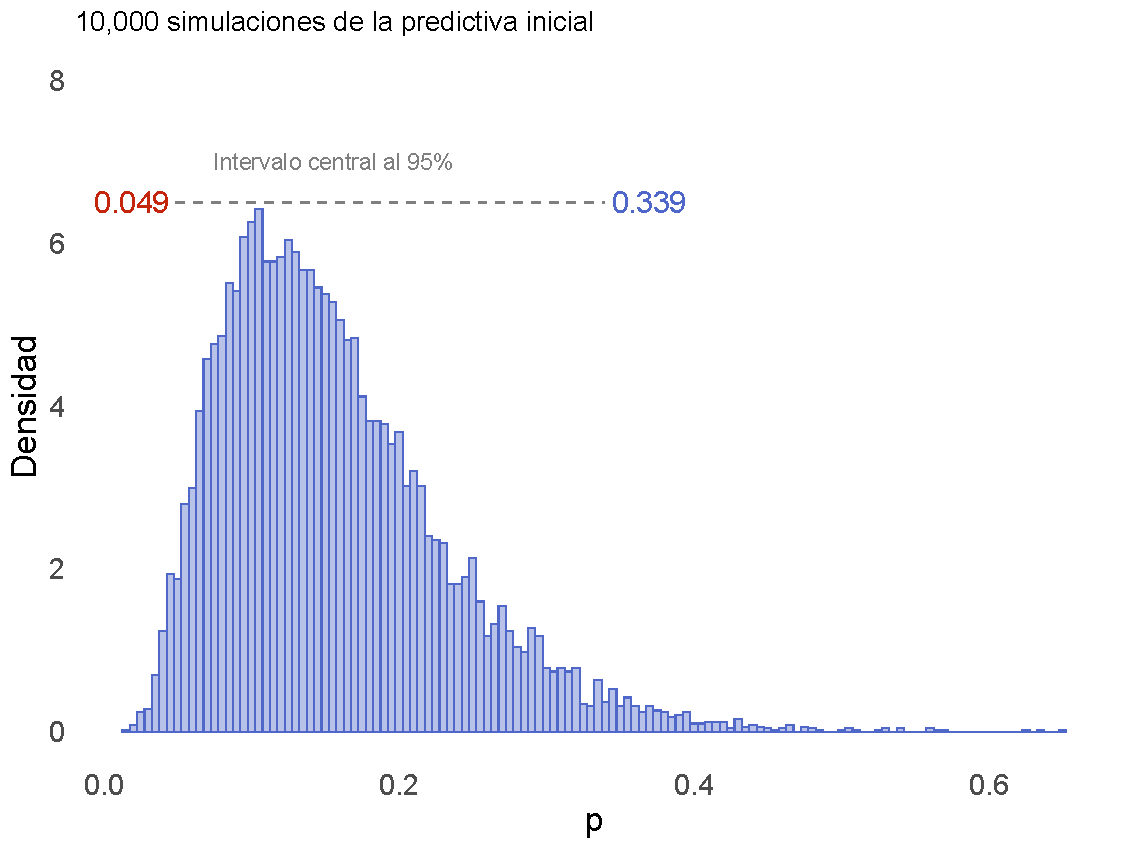
\includegraphics[width = 0.8\textwidth]{Figs/Modelado/Pred_Inicial}
	\caption{Fuente: elaboración propia.}
	\label{fig:Predictiva_Inicial}
\end{figure}

Estas distribuciones iniciales, como ya he mencionado, son subjetivas. Alguien más podría no estar muy convencido de la elección que realizo, por lo que eran importantes los párrafos anteriores de manera que fuera más transparente el proceso por el cual llegué a elegirlas.\\  

\section{Modelos individuales}

Consideremos entonces, para cada variable explicativa, modelos de la siguiente forma:

\begin{align}\label{eq:Modelo_Nal_Ind}
y_c|\theta=(\alpha,\beta) & \sim Binom(n_c,p_c) \quad \forall \quad c \in \mathbb{N}_C \nonumber \\
\text{con} \quad ln\left(\dfrac{p_c}{1-p_c}\right) &= \alpha + \sum\limits_{j=1}^{l_m} \beta_j x_{j,c} \quad \text{tal que} \quad \beta_{l_m} = -\sum\limits_{k = 1}^{l_m} \beta_k \nonumber \\
\text{y} \quad \alpha & \sim N(\mu = -1.7,\sigma = 0.25) \nonumber \\
\beta_j & \sim N(\mu = 0,\sigma = 0.5) \quad \, j \in \mathbb{N}_{l_m-1} 
\end{align}

A \eqref{eq:Modelo_Nal_Ind} le llamaré un \textbf{Modelo Nacional Individual} porque se tienen coeficientes a nivel nacional\footnote{En realidad, como mencionaba en el análisis exploratorio de datos, son coeficientes para la metrópoli y no para todo el país.} y solo incluyo una variable explicativa de manera individual. Tendría entonces 9 modelos nacionales individuales de esta forma. Sin embargo, el análisis exploratorio de datos sugería que se podría modelar de mejor manera dejando que los coeficientes e interceptos variasen para cada uno de los 96 departamentos. Es decir, podríamos construir igualmente 9 \textbf{Modelos Jerárquicos Individuales}. Si denotamos como $d[c]$ el \textit{departamento} al que pertenece la comuna $c$, el modelo jerárquico individual sería: 

\begin{align}\label{eq:Modelo_Jer_Ind}
y_c|\theta & \sim Binom(n_c,p_c) \quad \forall \, c \in \mathbb{N}_C \nonumber \\
\text{con} \quad ln\left(\dfrac{p_c}{1-p_c}\right) &= \alpha_{d[c]} + \sum\limits_{j=1}^{l_m} \beta_{d[c],j} x_{j,c} \nonumber\\ 
\text{tal que} \quad \beta_{d,l_m} &= -\sum\limits_{k = 1}^{l_m} \beta_{d,k} \nonumber \\
\alpha_d & \sim N(\mu_{\alpha}, \sigma=1) \quad \forall \, d \in \mathbb{N}_{96} \nonumber \\
\beta_{d,j} & \sim N(\mu_{\beta}, \sigma=1) \quad \forall \, j \in \mathbb{N}_{l_m-1}  \quad \text{y} \quad d \in \mathbb{N}_{96} \nonumber \\
\mu_{\alpha} &\sim N(-1.7,\sigma=0.25) \nonumber \\
\mu_{\beta} &\sim N(0,\sigma=0.5)
\end{align}

Se corrieron cada uno de los 18 modelos mediante el software Stan, simulando vía \textit{Hamiltonian Monte Carlo} las distribuciones posteriores dada la muestra de datos discutida en la \autoref{secc:muestra}. Una vez con dichas distribuciones posteriores, podemos hacer lo que \textcite{Gelman13} llaman \textit{posterior predictive checks}. Podemos predecir el porcentaje esperado de votos en cada una de las comunas y calcular su error respecto al real. Para el modelo nacional de ocupación laboral juvenil, los resultados están en la \textbf{Figura \ref{fig:Modelo_Nal_Ocu_Juvenil}}.\\

\begin{figure}[h]
	\centering
	\includegraphics[width = 0.8\textwidth]{Figs/Modelado/Modelo_Nal_Ocu_Juvenil}
	\caption{Mapa de predicciones medias del porcentaje bruto de votos obtenido por Marine Le Pen en las presidenciales 2012 mediante el Modelo Nacional por Ocupación Juvenil y mapa de los respectivos errores. Fuente: elaboración propia.}
	\label{fig:Modelo_Nal_Ocu_Juvenil}
\end{figure}

En el mapa de la izquierda las predicciones se colorean de acuerdo a la escala real que va de 0\% a 62.5\% y donde el cambio de tonos rojos a azules se da en la comuna mediana de 17.5\%. Observamos que la predicción en general subestima el verdadero porcentaje obtenido pues el mapa está prácticamente coloreado en su totalidad de tonos rojos. Sin embargo, las predicciones están cerca de la mediana. De hecho, el mapa de errores--- verde significa poco error y naranjas y rojos más--- visualmente es prácticamente un negativo del verdadero mapa de resultados que observábamos en la \textbf{Figura \ref{fig:Mapa_Pct_Br}} del capítulo anterior.\\

En general, los modelos nacionales tienen el defecto de no reconocer la enorme variabilidad geográfica del fenómeno electoral. Si construimos distintas medidas de error de predicción vemos que pasar de un modelado nacional a un modelado jerárquico las reduce consistentemente. Para cada simulación posterior predecimos el número de votos en cada comuna, departamento y a nivel nacional. Luego lo convertimos en porcentaje bruto de votos predicho dividiendo entre el número de inscritos en la comuna. Así, podemos tomar los conocidos errores absoluto y cuadrático promedio para el porcentaje de votos a nivel comuna, departamento y nacional. Incluso podemos tomar una pérdida más arbitraria, pero ilustrativa, como el porcentaje promedio de estimaciones que se encuentran a más de 1.5 puntos porcentuales del verdadero valor en los 3 niveles de agregación; a esta medida la llamo tolerancia 1.5 pp. Finalmente se calcula el promedio de las medidas a través del total de simulaciones posteriores y se grafican en la \textbf{Figura \ref{fig:Errores_Modelos_Individuales}}. El gráfico también incluye el cálculo de un cuarto error llamado WAIC para las comunas, pero a él me refiriré más adelante. En el gráfico, los puntos son las medidas para el modelo nacional y las flechas las de los modelos jerárquicos.\\ 

\begin{figure}[h]
	\centering
	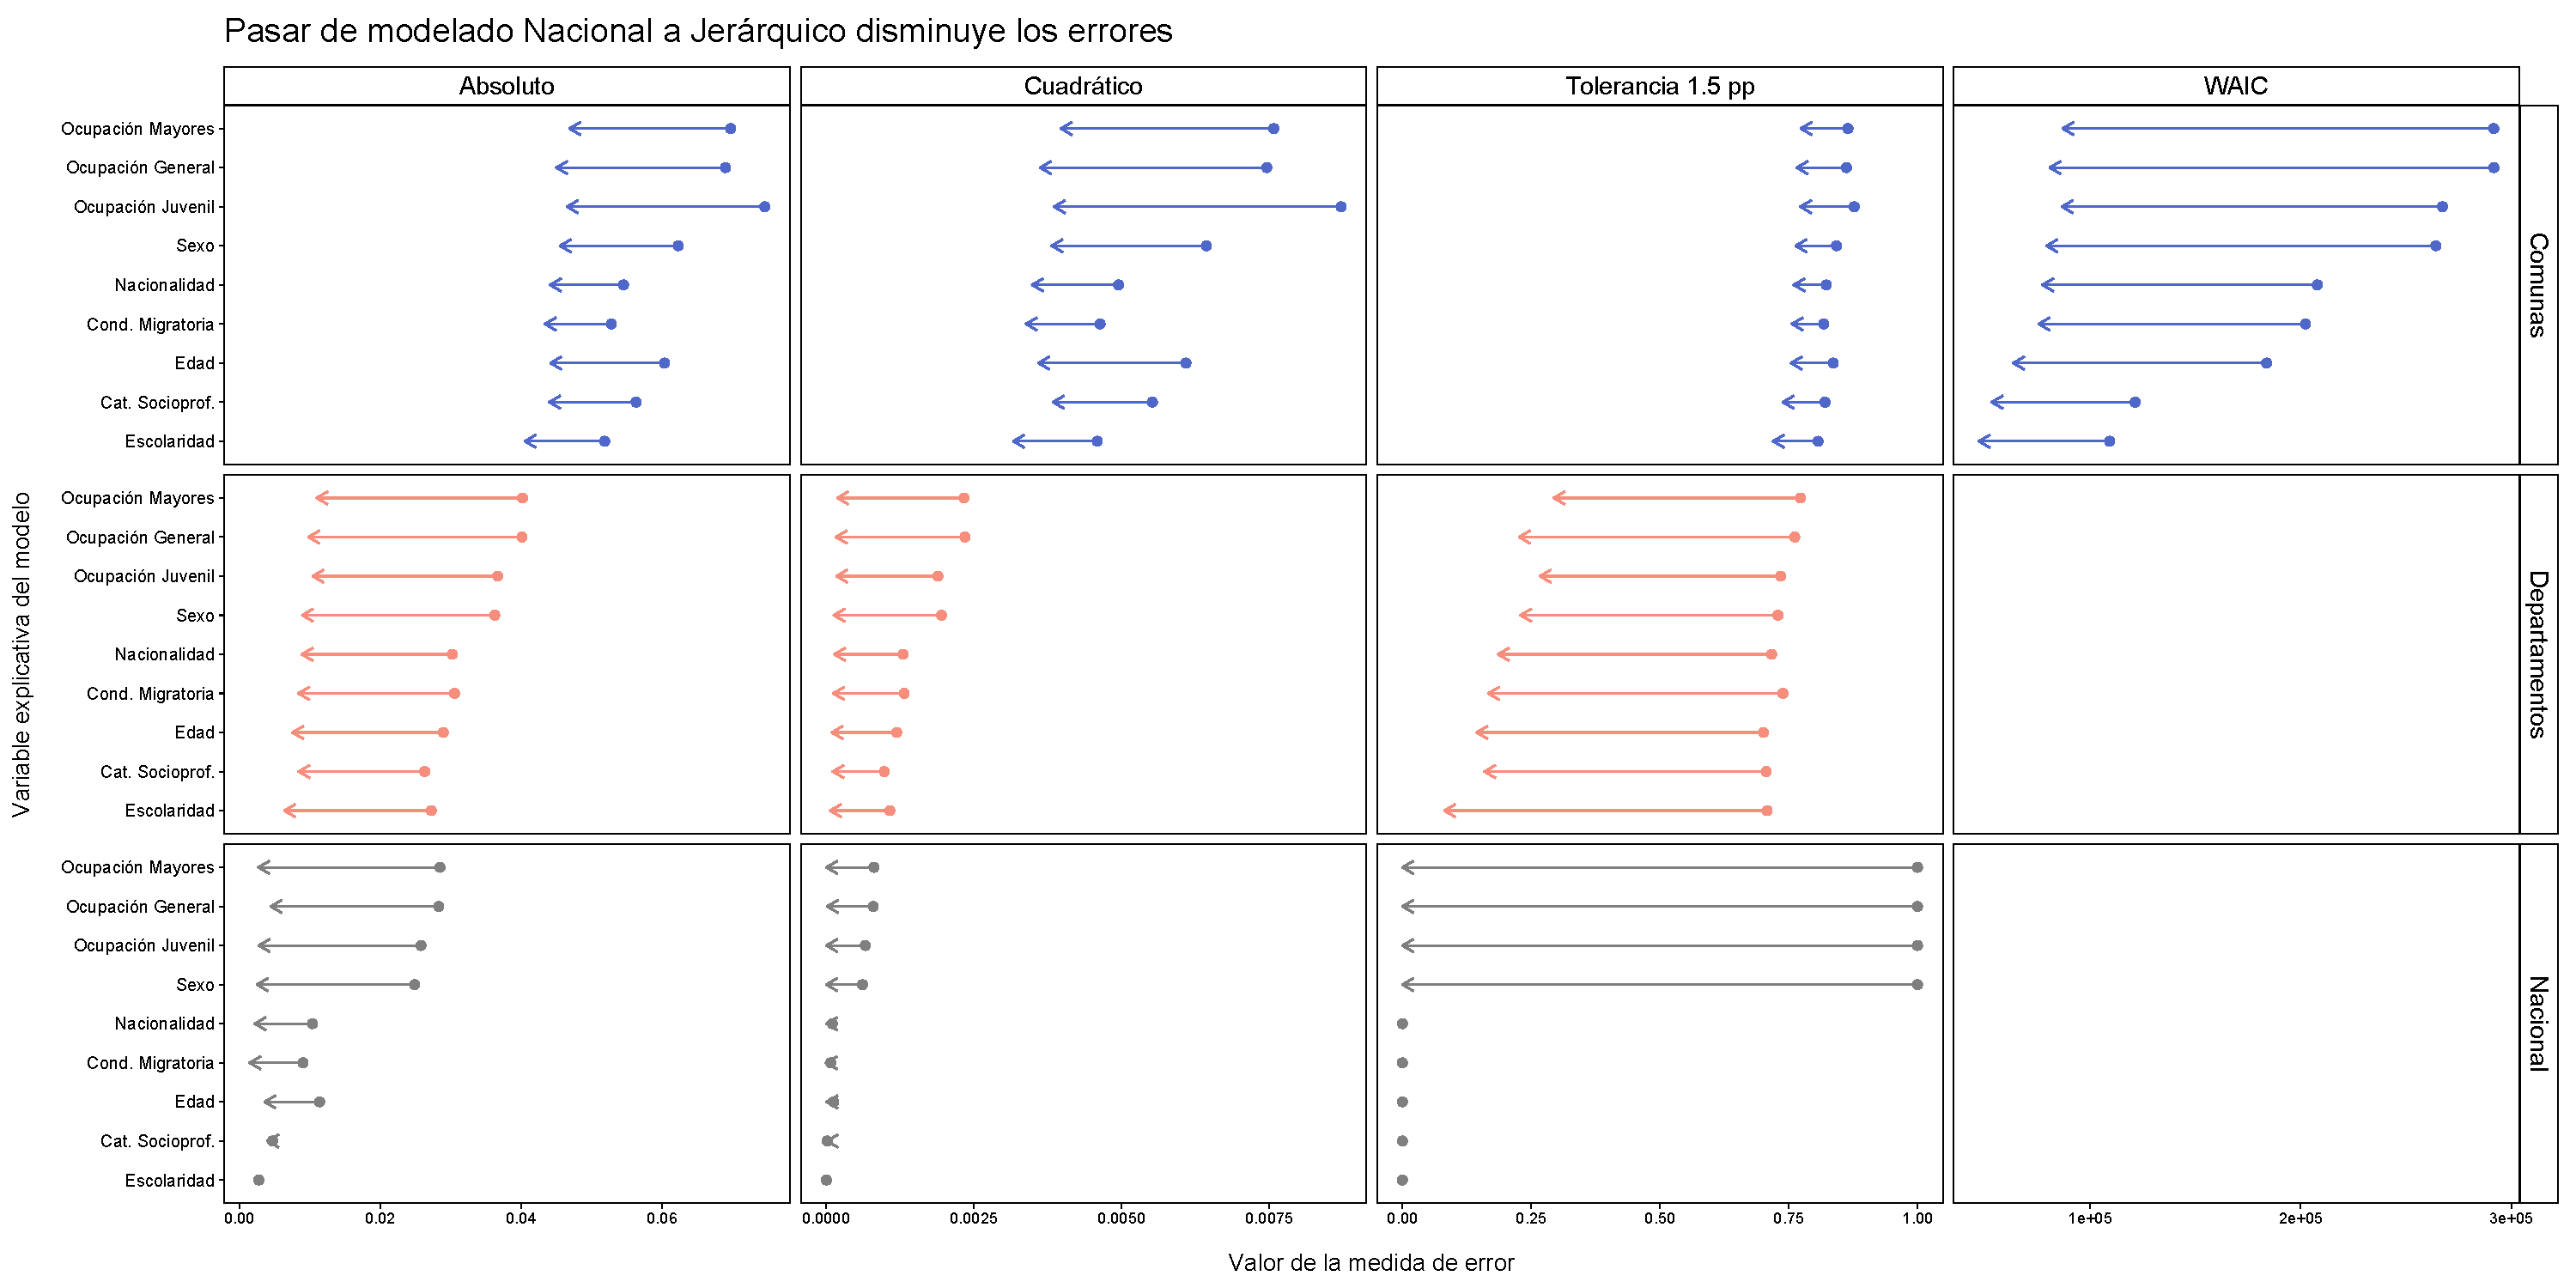
\includegraphics[width = 0.8\textwidth]{Figs/Modelado/Graf_Errores_Modelos_Individuales}
	\caption{Comparación de los modelos nacionales y jerárquicos individuales bajo diferentes medidas de error. Fuente: elaboración propia.}
	\label{fig:Errores_Modelos_Individuales}
\end{figure} 

Como es de esperarse, los modelos estiman de mejor manera los porcentajes de niveles de mayor agregación que el del nivel comunal. Viendo la pérdida arbitraria llamada de tolerancia 1.5, salvo las variables de sexo y ocupaciones, todas las predicciones estiman un porcentaje de votos nacional a menos de 1.5 puntos porcentuales del real. Sin embargo, vemos que para los 96 departamentos, los modelos nacionales solo logran esta precisión esperada de estimación en al rededor de 70. Esto refleja lo que había mencionado al ver el mapa de predicciones para el modelo nacional individual por ocupación juvenil. Al no permitir que los coeficientes varíen por departamento, el modelo ajusta para el país entero, sacrificando las estimaciones en las diferentes zonas geográficas que estos constituyen. Si observamos medidas de error más tradicionales como la absoluta o la cuadrática vemos que todas las flechas se dirigen a la izquierda, es decir que se reducen los errores al reconocer esa variabilidad geográfica. Ahora bien, estas 3 medidas tienen más un carácter ilustrativo y sirven para recordar que se pueden construir diferentes errores para diferentes estimadores.\\ 

Ahora notemos que las variables de solo 2 categorías como ocupación, sexo, nacionalidad y condición migratoria tienen peor desempeño que las de más categorías como edad, categoría socioprofesional y escolaridad. ¿Esto quiere decir que son peores variables explicativas? ¿No podría esto deberse a que las últimas tienen más parámetros y es más fácil ajustar mejor simplemente por introducir parámetros adicionales?\\

\subsection{WAIC}

Pensando en la posibilidad de mejorar un ajuste simplemente haciendo más complejo el modelo es que una mejor y más aceptada medida de error es el llamado WAIC por sus siglas en inglés \textit{Widely Applicable} o \textit{Watanabe-Akaike Information Criterion} \parencite{Vehtari16}. El WAIC busca estimar la capacidad predictiva de un modelo via las predictivas posteriores de los datos con los que se ajusta. La intuición es que a mayor valor de la predictiva posterior para el dato observado, mayor la posibilidad de predecir otros datos.\\ 

Para un conjunto de $n$ datos $y=(y_1,\dots,y_n)$ y una muestra posterior de parámetros $\left\lbrace\theta_{(s)}\right\rbrace_{s=1}^S$, el WAIC se define de la siguiente manera:

\begin{align}\label{WAIC}
WAIC(y|\theta) &= \widehat{lpd} + \widehat{par} \\
\text{con} \quad \widehat{lpd} &= \sum_{i=1}^{n} ln\left(\dfrac{1}{S}\sum\limits_{s=1}^S f(y_i|\theta_{(s)}) \right) \nonumber \\
\text{y} \quad \widehat{par} &= \sum\limits_{i=1}^n V(y_i|\theta), \nonumber
\end{align}

donde $V(y_i|\theta)=\dfrac{1}{S-1}\sum\limits_{s=1}^S \mathcal{L}(y_i;\theta_{s})^2$ y $\mathcal{L}(y_i;\theta_{s}) = ln\left[f(y_i|\theta_{(s)})\right] - \dfrac{1}{S}\sum\limits_{s=1}^S ln\left[f(y_i|\theta_{(s)})\right]$.{}\\

El WAIC se conforma de dos sumas. La primera, $\widehat{lpd}$, es una aproximación de la log predictiva posterior, es decir una medidad de ajuste. Por otro lado, $\widehat{par}$ es normalmente llamado el \textit{número efectivo estimado de parámetros} y es una medida que mediante sumas de varianzas busca medir la complejidad del modelo. En total, entre menor sea el valor del WAIC, esperaríamos un mejor desempeño predictivo tomando en cuenta la complejidad del modelo.\\ 

Notemos que con la definición dada, el WAIC es un estimador por lo que tiene una distribución muestral. Gracias al paquete \textit{loo} de $\mathsf{R}$, podemos estimar tanto los WAICs y sus errores estándar como la diferencia esperada entre dos de ellos y, {\color{Red} argumentando un teorema central del límite, la probabilidad de que el WAIC de un modelo sea efectivamente menor o igual al WAIC de otro. Estas comparaciones las observamos en la \textbf{Figura \ref{fig:Compara_WAIC_Individuales}}.}\\

\begin{figure}[h]
	\centering
	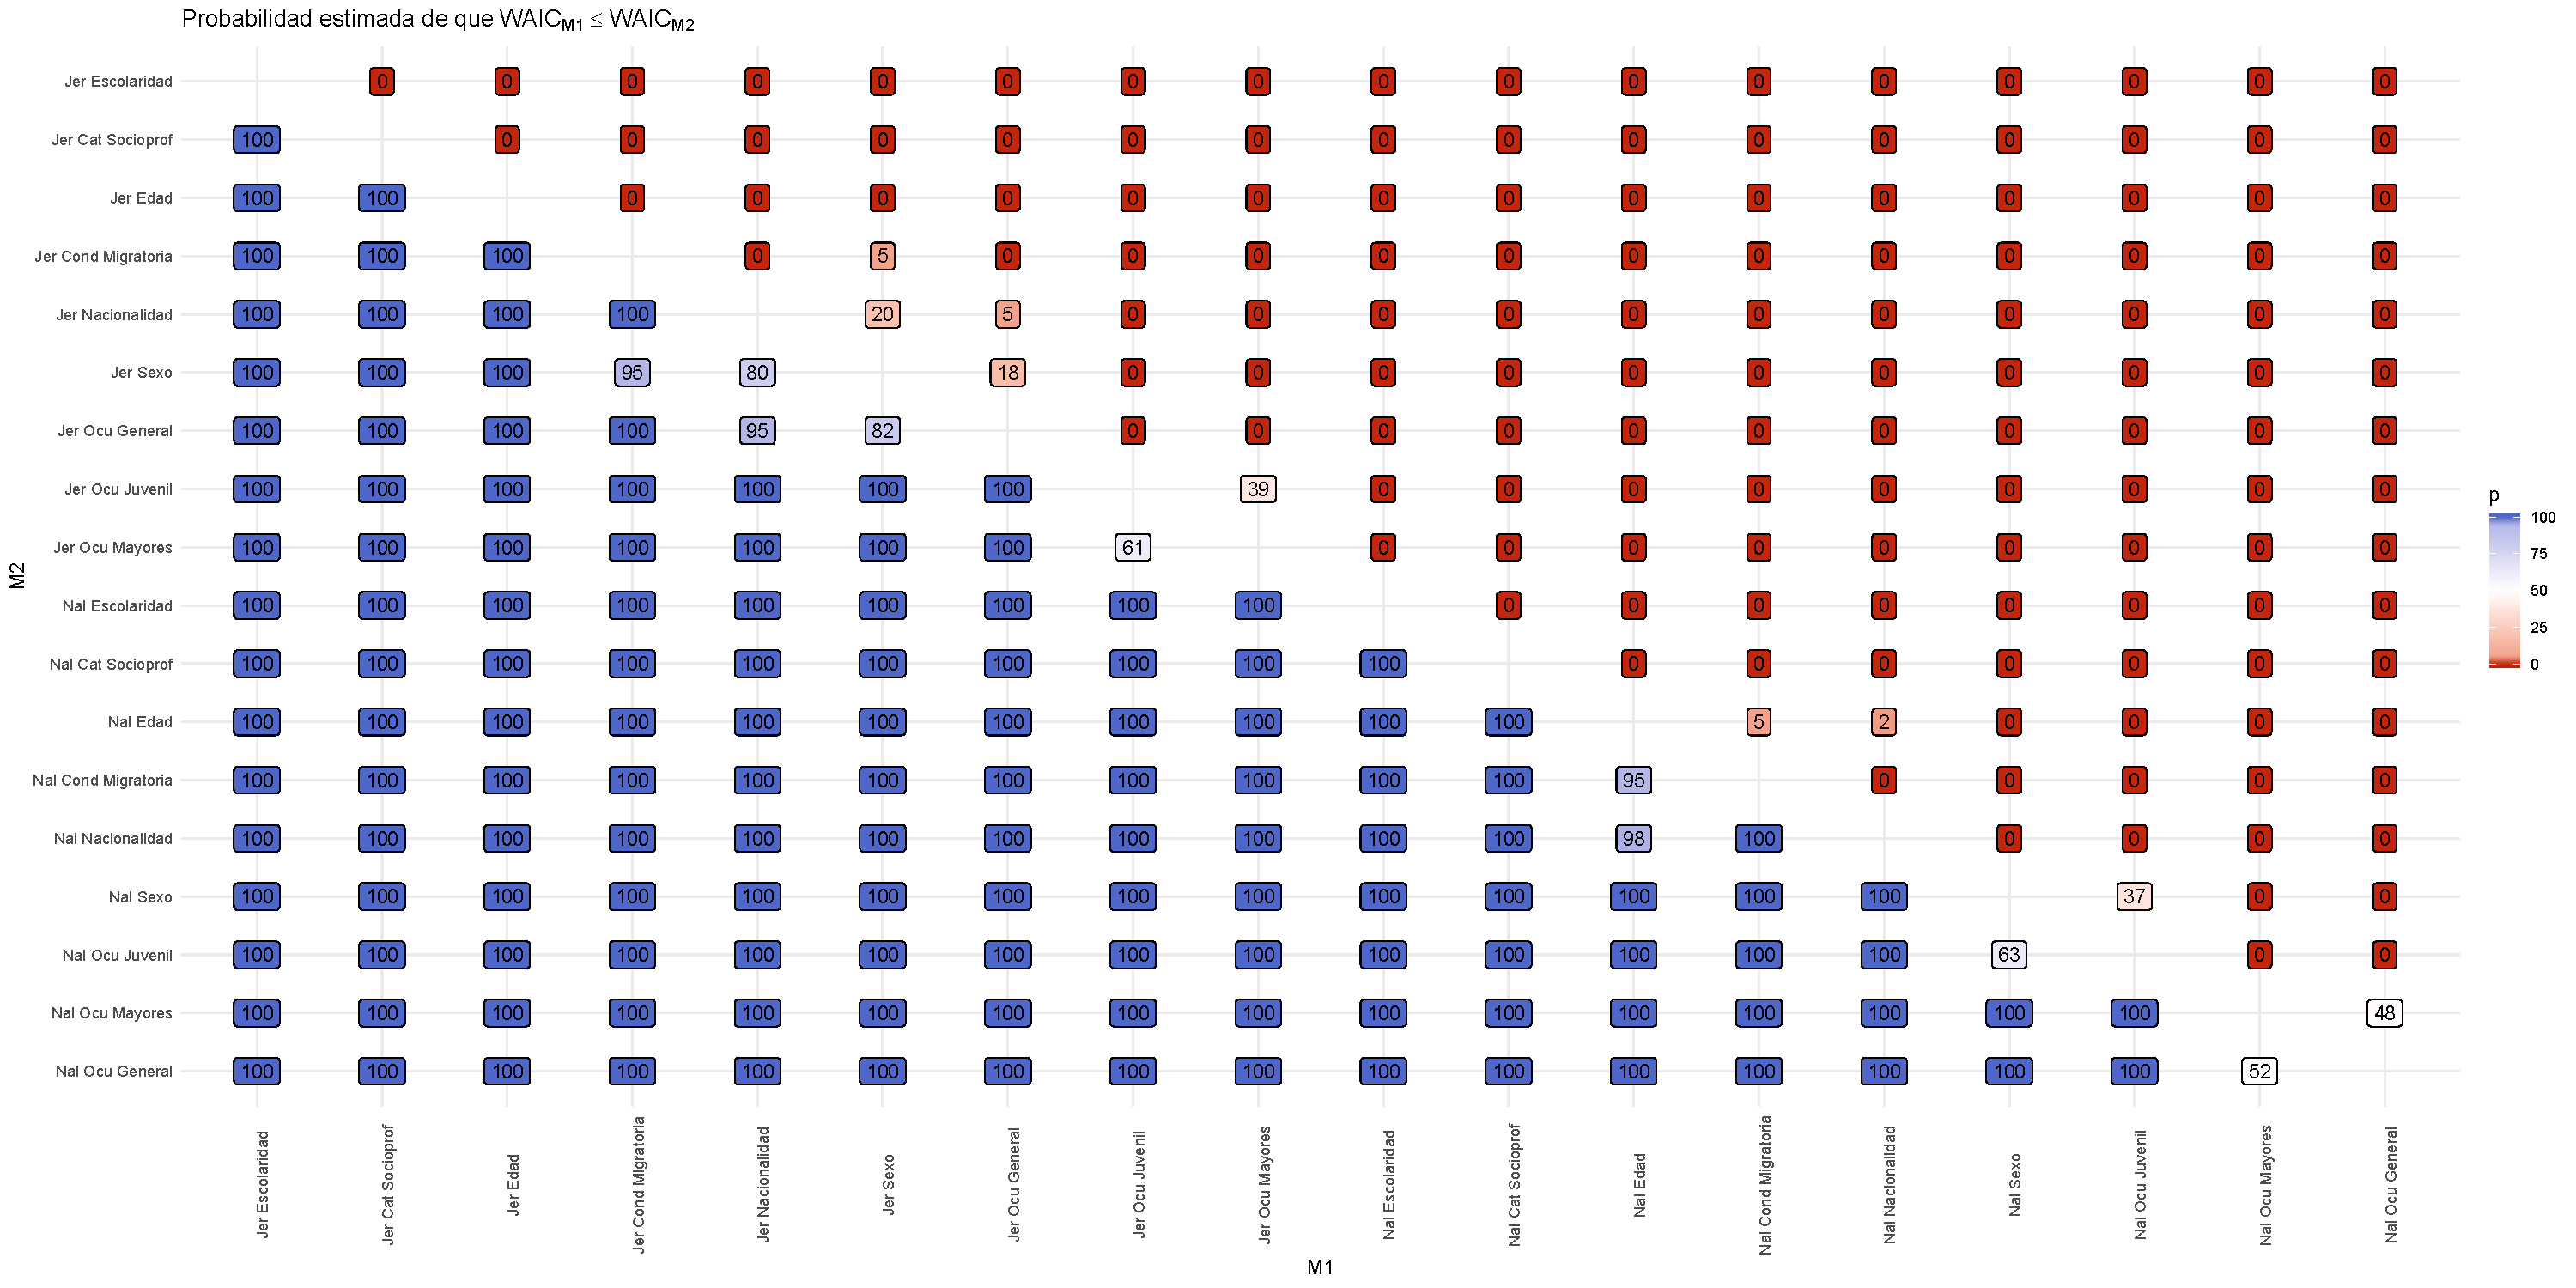
\includegraphics[width = 0.9\textwidth]{Figs/Modelado/Graf_WAIC_Probas_Modelos_Individuales}
	\caption{Comparativo de WAIC para distintos modelos. Fuente: elaboración propia con base en la estimación de la diferencia en WAIC proveniente de la función \textit{compare} del paquete \textit{loo} dentro $\mathsf{R}$ y asumiendo una distribución normal para la diferencia.}
	\label{fig:Compara_WAIC_Individuales}
\end{figure}

Para la mayoría de las comparaciones es claro que un modelo tiene mejor ajuste que el otro. Podríamos pensar que efectivamente hay un ordenamiento en el poder predictivo de las distintas variables: escolaridad, categorías socioprofesionales, edad, condición migratoria, nacionalidad, sexo y, finalmente, las ocupaciones. Sin concluir todavía nada, parecería que a las hipótesis sobre inseguridad laboral no les corresponde el mejor de los poderes explicativos en términos de estos modelos.\\

\section{Modelos compuestos}

Este ordenamiento preliminar tiene el objetivo de ayudarme a construir, secuencialmente, un modelo cada vez más complejo. Para comenzar, veamos los mapas de predicción que generó el modelo con menor WAIC, el jerárquico por escolaridad, en la \textbf{Figura \ref{fig:Modelo_Jer_Escolaridad}}.\\ 

\begin{figure}[h]
	\centering
	\includegraphics[width = 0.8\textwidth]{Figs/Modelado/Modelo_Jer_Escolaridad}
	\caption{Mapa de predicciones medias del porcentaje bruto de votos obtenido por Marine Le Pen en las presidenciales 2012 mediante el Modelo Jerárquico por Escolaridad y mapa de los respectivos errores. Fuente: elaboración propia.}
	\label{fig:Modelo_Jer_Escolaridad}
\end{figure}

El mapa de errores ya se observa más verde y homogéneo. Las grandes zonas de fortaleza y debilidad del FN comienzan a ser identificadas por el modelo. Sin embargo, los tonos de algunas predicciones son todavía demasiado cercanos a la mediana. En el centro observamos una zona de tonos muy claros, casi blancos, que no corresponden totalmente a la realidad. En general, vemos que hay menor variabilidad dentro de los departamentos de la que se observó en la elección.\\ 

Estas reflexiones sugieren que, en lugar de tomar una a una las variables, podemos ir agregando variables a la regresión en modelos jerárquicos secuenciales que refinen el ajuste. Entonces, este modelo jerárquico por escolaridad podríamos considerarlo el \textbf{Modelo 0}, pues partiremos de él para ir agrandándolo con la inclusión de una nueva variable cada vez.\\ 

El primer modelo compuesto incluye las variables de escolaridad y categorías socioprofesionales. A este modelo lo llamaré el \textbf{Modelo A}. Para distinguir las variables utilizaré diferentes letras griegas para sus coeficientes. Para la configuración social de escolaridad 
\[x_{escol,c} = (Esc_c,Dip1_c,Dip2_c,Dip3_c,Dip4_c)^T\]
en la comuna $c$ los coeficientes departamentales serán un vector $\beta_{d[c]} = (\beta_{d[c],1},\dots,\beta_{d[c],5})$. Para las categorías socioprofesionales $x_{csp,c}$ los coeficientes serán $\gamma_{d[c]}$:

\begin{align}\label{eq:Modelo_Comp_A}
y_c|\theta & \sim Binom(n_c,p_c) \quad \forall \, c \in \mathbb{N}_C \nonumber \\
\text{con} \quad ln\left(\dfrac{p_c}{1-p_c}\right) &= \alpha_{d[c]} + \beta_{d[c]} x_{escol,c} + \gamma_{d[c]} x_{csp,c} \\ 
\intertext{tal que} 
\beta_{d,5} &= -\sum\limits_{k = 1}^{4} \beta_{d,k}, \nonumber \\
\gamma_{d,8} &= -\sum\limits_{k = 1}^{7} \gamma_{d,k} \nonumber \\
\intertext{donde $\forall \, d \in \mathbb{N}_{96}$}
\alpha_d & \sim N(\mu_{\alpha}, \sigma=1) \quad  \nonumber \\
\beta_{d,j} & \sim N(\mu_{\beta}, \sigma=1) \quad \forall \, j \in \mathbb{N}_{4} \nonumber \\
\gamma_{d,j} & \sim N(\mu_{\gamma}, \sigma=1) \quad \forall \, j \in \mathbb{N}_{7} \nonumber \\
\intertext{y}
\mu_{\alpha} &\sim N(-1.7,\sigma=0.25) \nonumber \\
\mu_{\beta} &\sim N(0,\sigma=0.5) \nonumber \\
\mu_{\gamma} &\sim N(0,\sigma=0.5) \nonumber
\end{align}

Al estimar el modelo con ambas variables las predicciones efectivamente mejoran. La diferencia en WAIC entre el modelo A y el modelo jerárquico por escolaridad se estima en -1594.7 con un error estándar de 175.2. Asimismo, observando los mapas de la \textbf{Figura \ref{fig:Modelo_Compuesto_A}}, vemos que se reduce la gran zona blanquiza del centro, se comienza a observar mayor variabilidad dentro de los departamentos y los tonos también se oscurecen más, sobre todo en el noreste.\\ 

\begin{figure}[h]
	\centering
	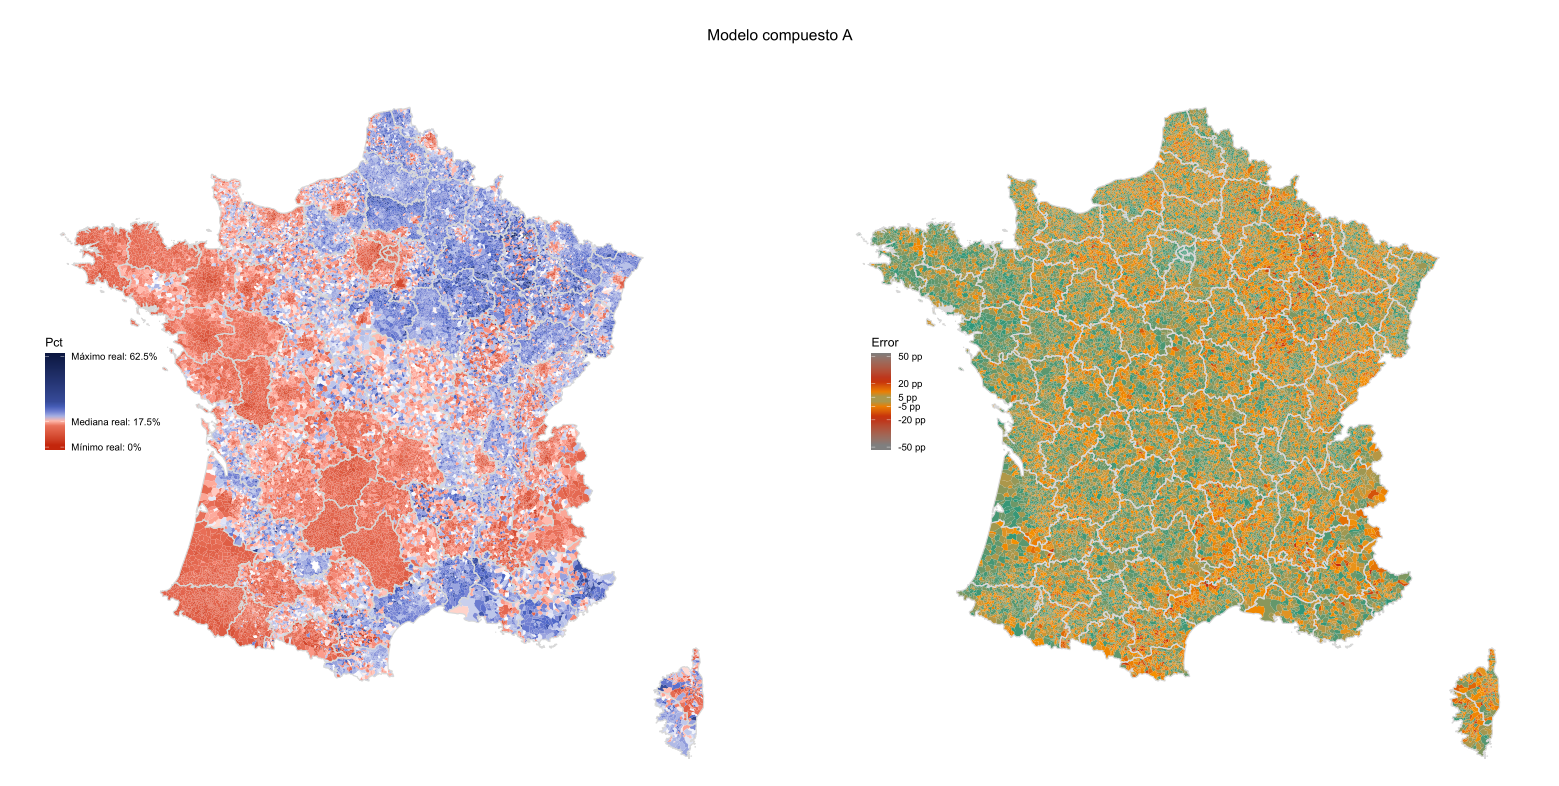
\includegraphics[width = 0.8\textwidth]{Figs/Modelado/Modelo_Compuesto_A}
	\caption{Mapas de predicciones medias y respectivos errores para el porcentaje bruto de votos obtenido por Marine Le Pen en las presidenciales 2012 mediante el Modelo Jerárquico por Escolaridad y Categorías socioprofesionales. Fuente: elaboración propia.}
	\label{fig:Modelo_Compuesto_A}
\end{figure}


Los siguientes modelos se llamarán de manera progresiva por letras latinas y sus planteamientos en términos de ecuaciones pueden encontrarse en el \autoref{Anexo_modelos_compuestos}. Por ejemplo, el \textbf{Modelo B} incorpora los grupos de edad $x_{edad,c}$. Al hacerlo, el WAIC vuelve a disminuir, ahora 965.4 unidades. Debido a la similitud entre condición migratoria y nacionalidad, solamente buscaba incorporar una de las dos, tratando de identificar la que tuviera mejor desempeño. De acuerdo al ordenamiento previo en los modelos individuales, consideraré solo la variable migratoria $x_{migr,c}$ dentro del \textbf{Modelo C}. Por su parte, el \textbf{Modelo D} incluye la distribución comunal por sexo $x_{sexo,c}$. {\color{Red} No presento los mapas por brevedad, pero de necesitarse se incluyen pues ya están generados}.\\

Después comenzaríamos a incluir las variables de ocupación. Como mencionaba al presentarlas, tengo un interés especial en la (des)ocupación juvenil, pues esta sería una variable que referencias como \textcite{LeBras16} y \textcite{Perrineau07} favorecerían. Por ello, al margen del ordenamiento, construí dos modelos de 6 variables. De manera general ambos incorporan una variable explicativa $x_{ocu,c}$. El \textbf{Modelo E} es el modelo D más la ocupación juvenil, mientras que el \textbf{Modelo F} es el modelo D más la ocupación general. Una vez generados por separado, podemos considerar un modelo que incorpore ambas variables, este sería el \textbf{Modelo G}. Finalmente agregamos la última variable considerada, la ocupación para personas de 55 a 64 años $x_{ocu\_may,c}$, para obtener el \textbf{Modelo H}, cuyos mapas corresponden a la \textbf{Figura \ref{fig:Modelo_Compuesto_H}}.\\

\begin{figure}[h]
	\centering
	\includegraphics[width = 0.8\textwidth]{Figs/Modelado/Modelo_Compuesto_H}
	\caption{Mapas de predicciones medias y respectivos errores para el porcentaje bruto de votos obtenido por Marine Le Pen en las presidenciales 2012 mediante el Modelo Jerárquico por Escolaridad, Categorías socioprofesionales, Edad, Condición migratoria, Sexo y Ocupaciones. Fuente: elaboración propia.}
	\label{fig:Modelo_Compuesto_H}
\end{figure}

¿Cuál es la comparación de WAICs entre todos estos modelos? En la \textbf{Figura \ref{fig:Compara_WAIC_Compuestos}} podemos observarlo. En general, el WAIC mejora conforme se van agregando variables. Ciertamente las mayores ganancias se dan al agregar las primeras variables que el análisis individual sugería eran las más explicativas. Esto parece reforzar dicha hipótesis. Por el contrario, en términos de WAIC, la ocupación juvenil no parece ser la más poderosa de las variables. En efecto, la ganancia en WAIC frente al modelo D al agregarla en el modelo E es de apenas 46 unidades, menor a la ganancia del modelo F que fue de 162. Más aún, al pasar del modelo F al modelo G agregándola de nuevo, la ganancia vuelve a ser poca, apenas de 29. Esto no quiere decir, sin embargo, que no aporte nada a la regresión. Aunque la mejora en WAIC sea pequeña y los intervalos con error estándar se traslapen, {\color{Red} la probabilidad de que agregarla produce un mejor modelo es de 84\% en el caso del modelo E y de 77\% en el modelo G.}

\begin{figure}[h]
	\centering
	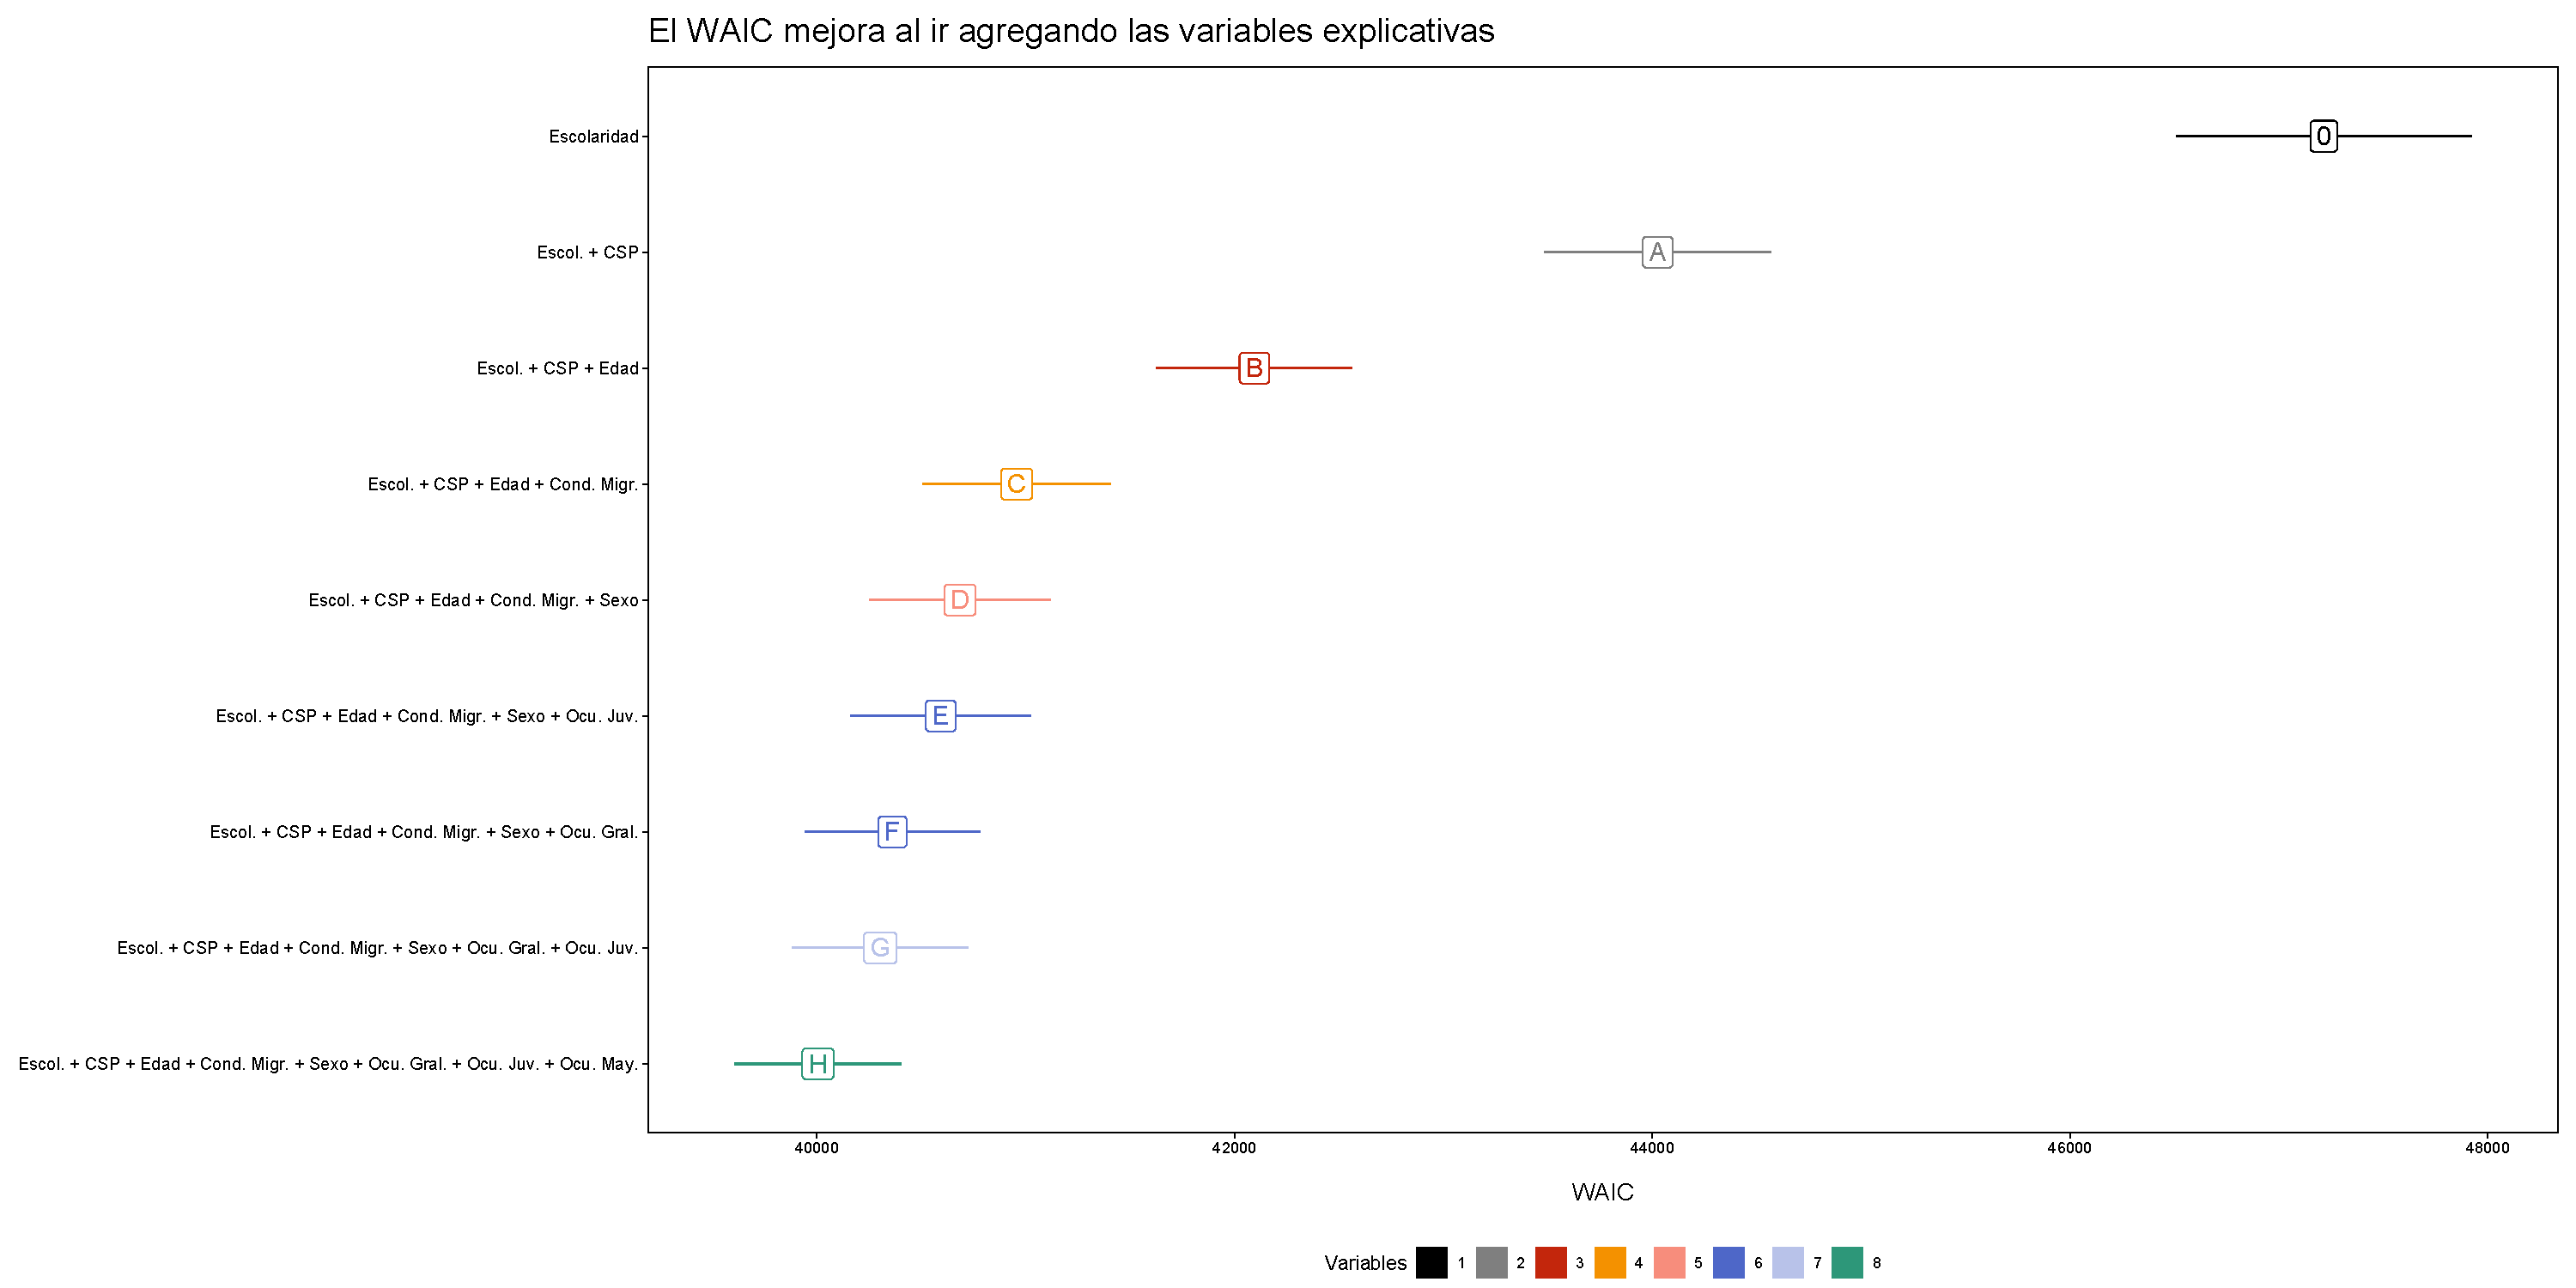
\includegraphics[width = 0.9\textwidth]{Figs/Modelado/Graf_WAIC_Modelos_Compuestos}
	\caption{Comparativo de WAIC para distintos modelos. Comenzando por el modelo 0 que incluye solo escolaridad se van añadiendo variables hasta incluirlas todas en el modelo H. Fuente: elaboración propia.}
	\label{fig:Compara_WAIC_Compuestos}
\end{figure}

\subsection{Convergencia de HMC}

Una vez ajustados los modelos, como adelantaba en la \autoref{sec:Convergencia}, habría que verificar que las cadenas simuladas mediante la implementación de HMC dentro de Stan hubieran convergido. Debido a la cantidad de parámetros dentro de cada modelo, así como a la cantidad de modelos ajustados en sí, es difícil verificar a detalle todas y cada una de las muestras posteriores. Afortunadamente, \textcite{BetancourtRStanWorkflow} desarrolla un caso de estudio en el que ilustra cómo programar distintos diagnósticos útiles para todos los parámetros de interés dentro de todos los modelos. Entre ellos encontramos el factor de reducción de escala $\hat{R}$, así como un cálculo del tamaño efectivo de muestra por iteración y 3 diagnósticos particulares de HMC. Utilizando su código abierto\footnote{Los derechos de autor son de Michael Betancourt y la Universidad de Columbia y las licencias específicas pueden verificarse en el link en las referencias.}, verificamos que los modelos satisfacen los criterios planteados y podemos confiar en la convergencia de las muestras posteriores obtenidas. {\color{Red} Esta comprobación puede reproducirse con el código del repositorio de Github de esta tesis y solicitándome acceso a los archivos .rds con los ajustes de todos los modelos.}\\

 Adicionalmente, podemos observar algunos diagnósticos gráficos para algunos parámetros del modelo H. Por ejemplo, en la \textbf{Figura \ref{fig:Traceplots_H}} observamos en los \textit{traceplots} que hay una buena mezcla de las cadenas; esto también se confirma viendo que las densidades por cadena de la \textbf{Figura \ref{fig:Densidades_H}} son parecidas. Finalmente, en la \textbf{Figura \ref{fig:Autocorr_H}} vemos que las autocorrelaciones son pequeñas. De hecho, existe un poco de simulación antitética que permite una mejor eficiencia en el tamaño de muestra \parencite{BlogAntithetical}.\\ 
 
 \begin{figure}[h]
	\centering
	\begin{subfigure}{0.45\textwidth}
	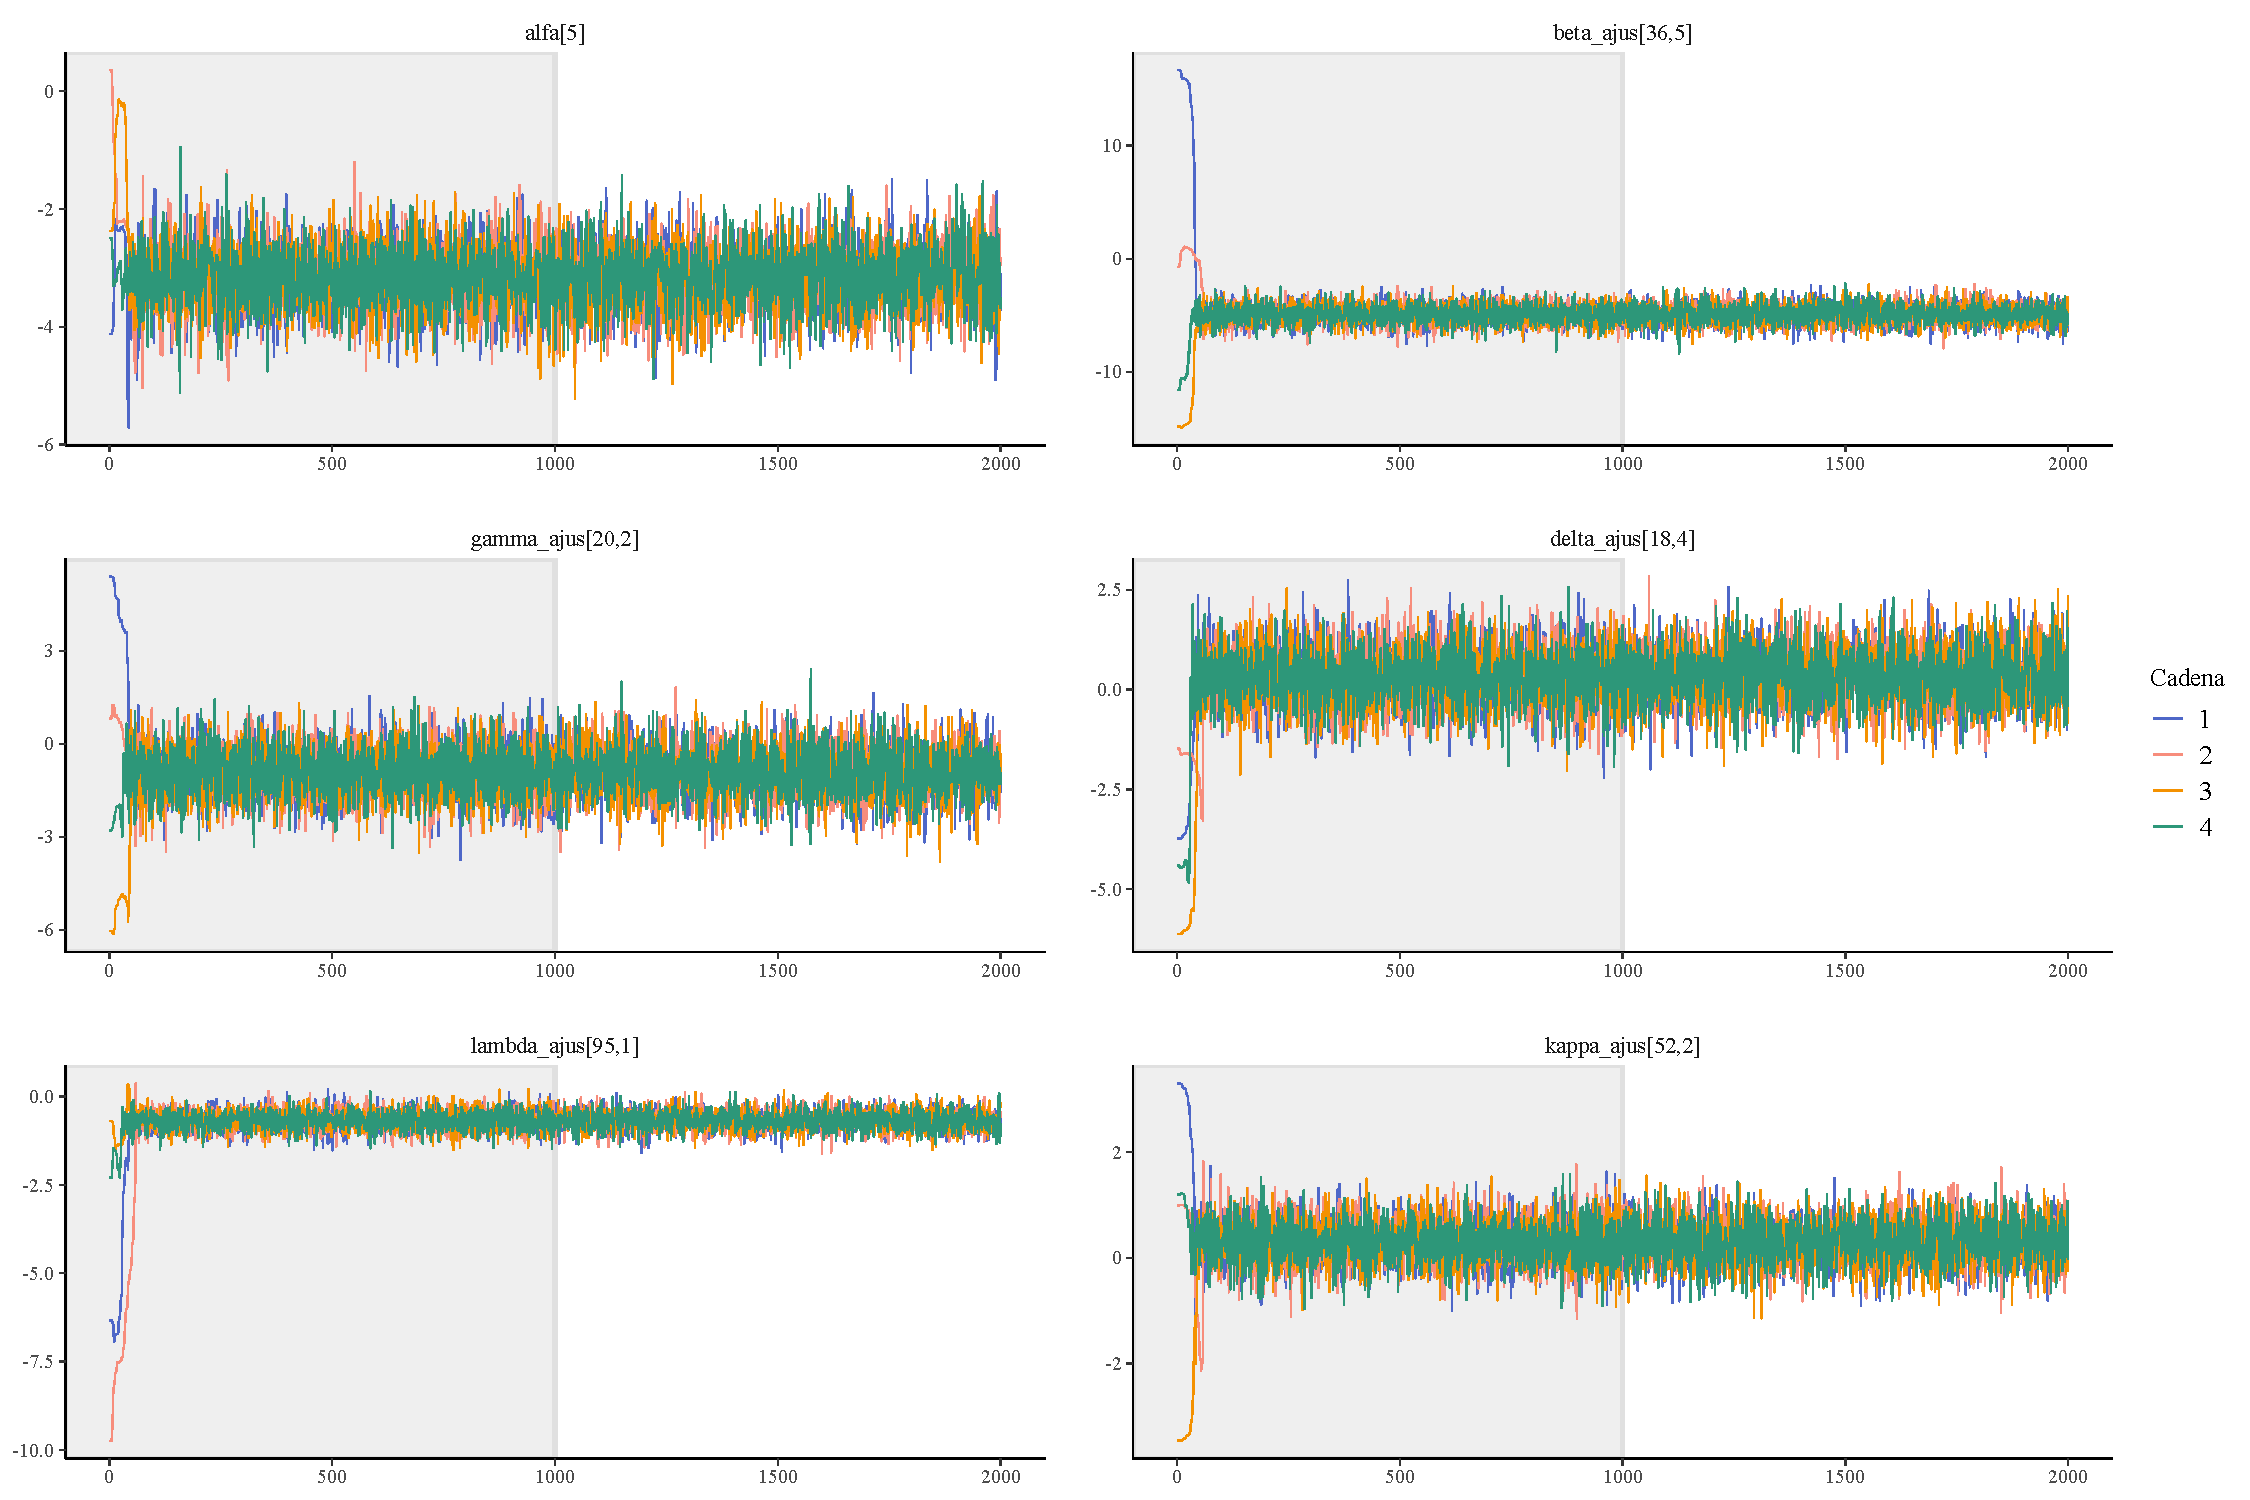
\includegraphics[width = \textwidth]{Figs/Convergencia/Convergencia_Traceplots}
	\caption{Ejemplo de \textit{traceplots} para algunos parámetros del modelo H.}
	\label{fig:Traceplots_H}
	\end{subfigure}
	~
	\begin{subfigure}{0.45\textwidth}
	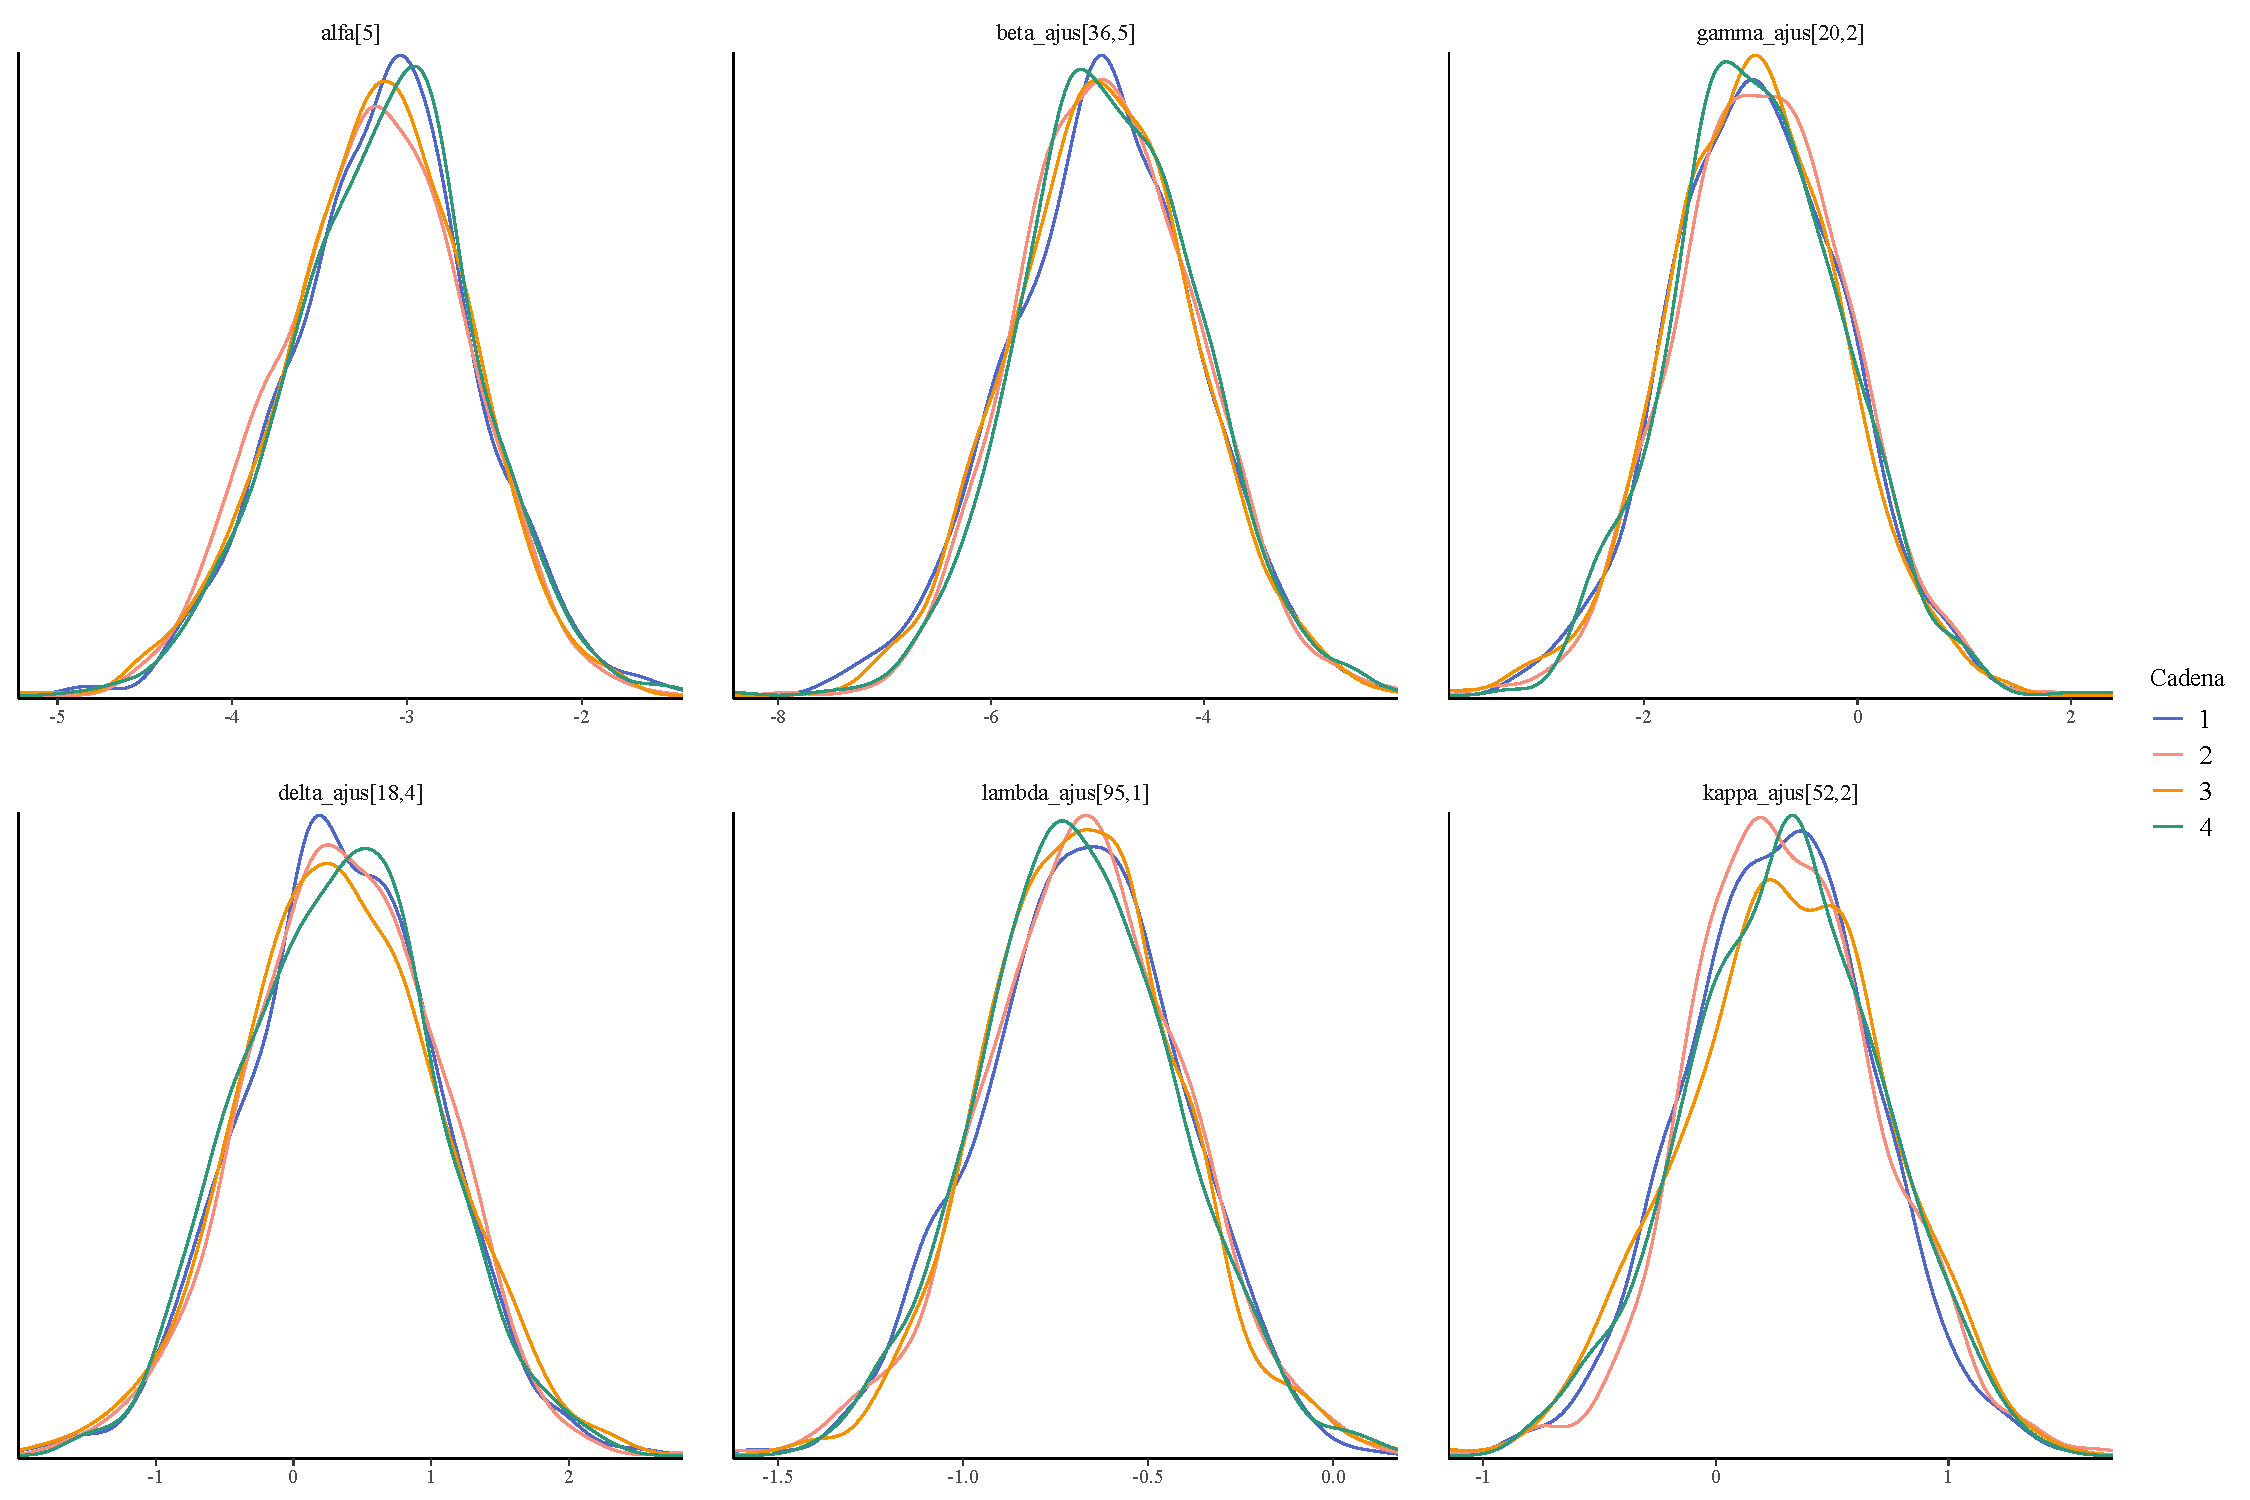
\includegraphics[width = \textwidth]{Figs/Convergencia/Convergencia_Densidades}
	\caption{Ejemplo de gráficos de densidades por cadena para algunos parámetros del modelo H.}
	\label{fig:Densidades_H}
	\end{subfigure}
	~
	\begin{subfigure}{0.6\textwidth}
	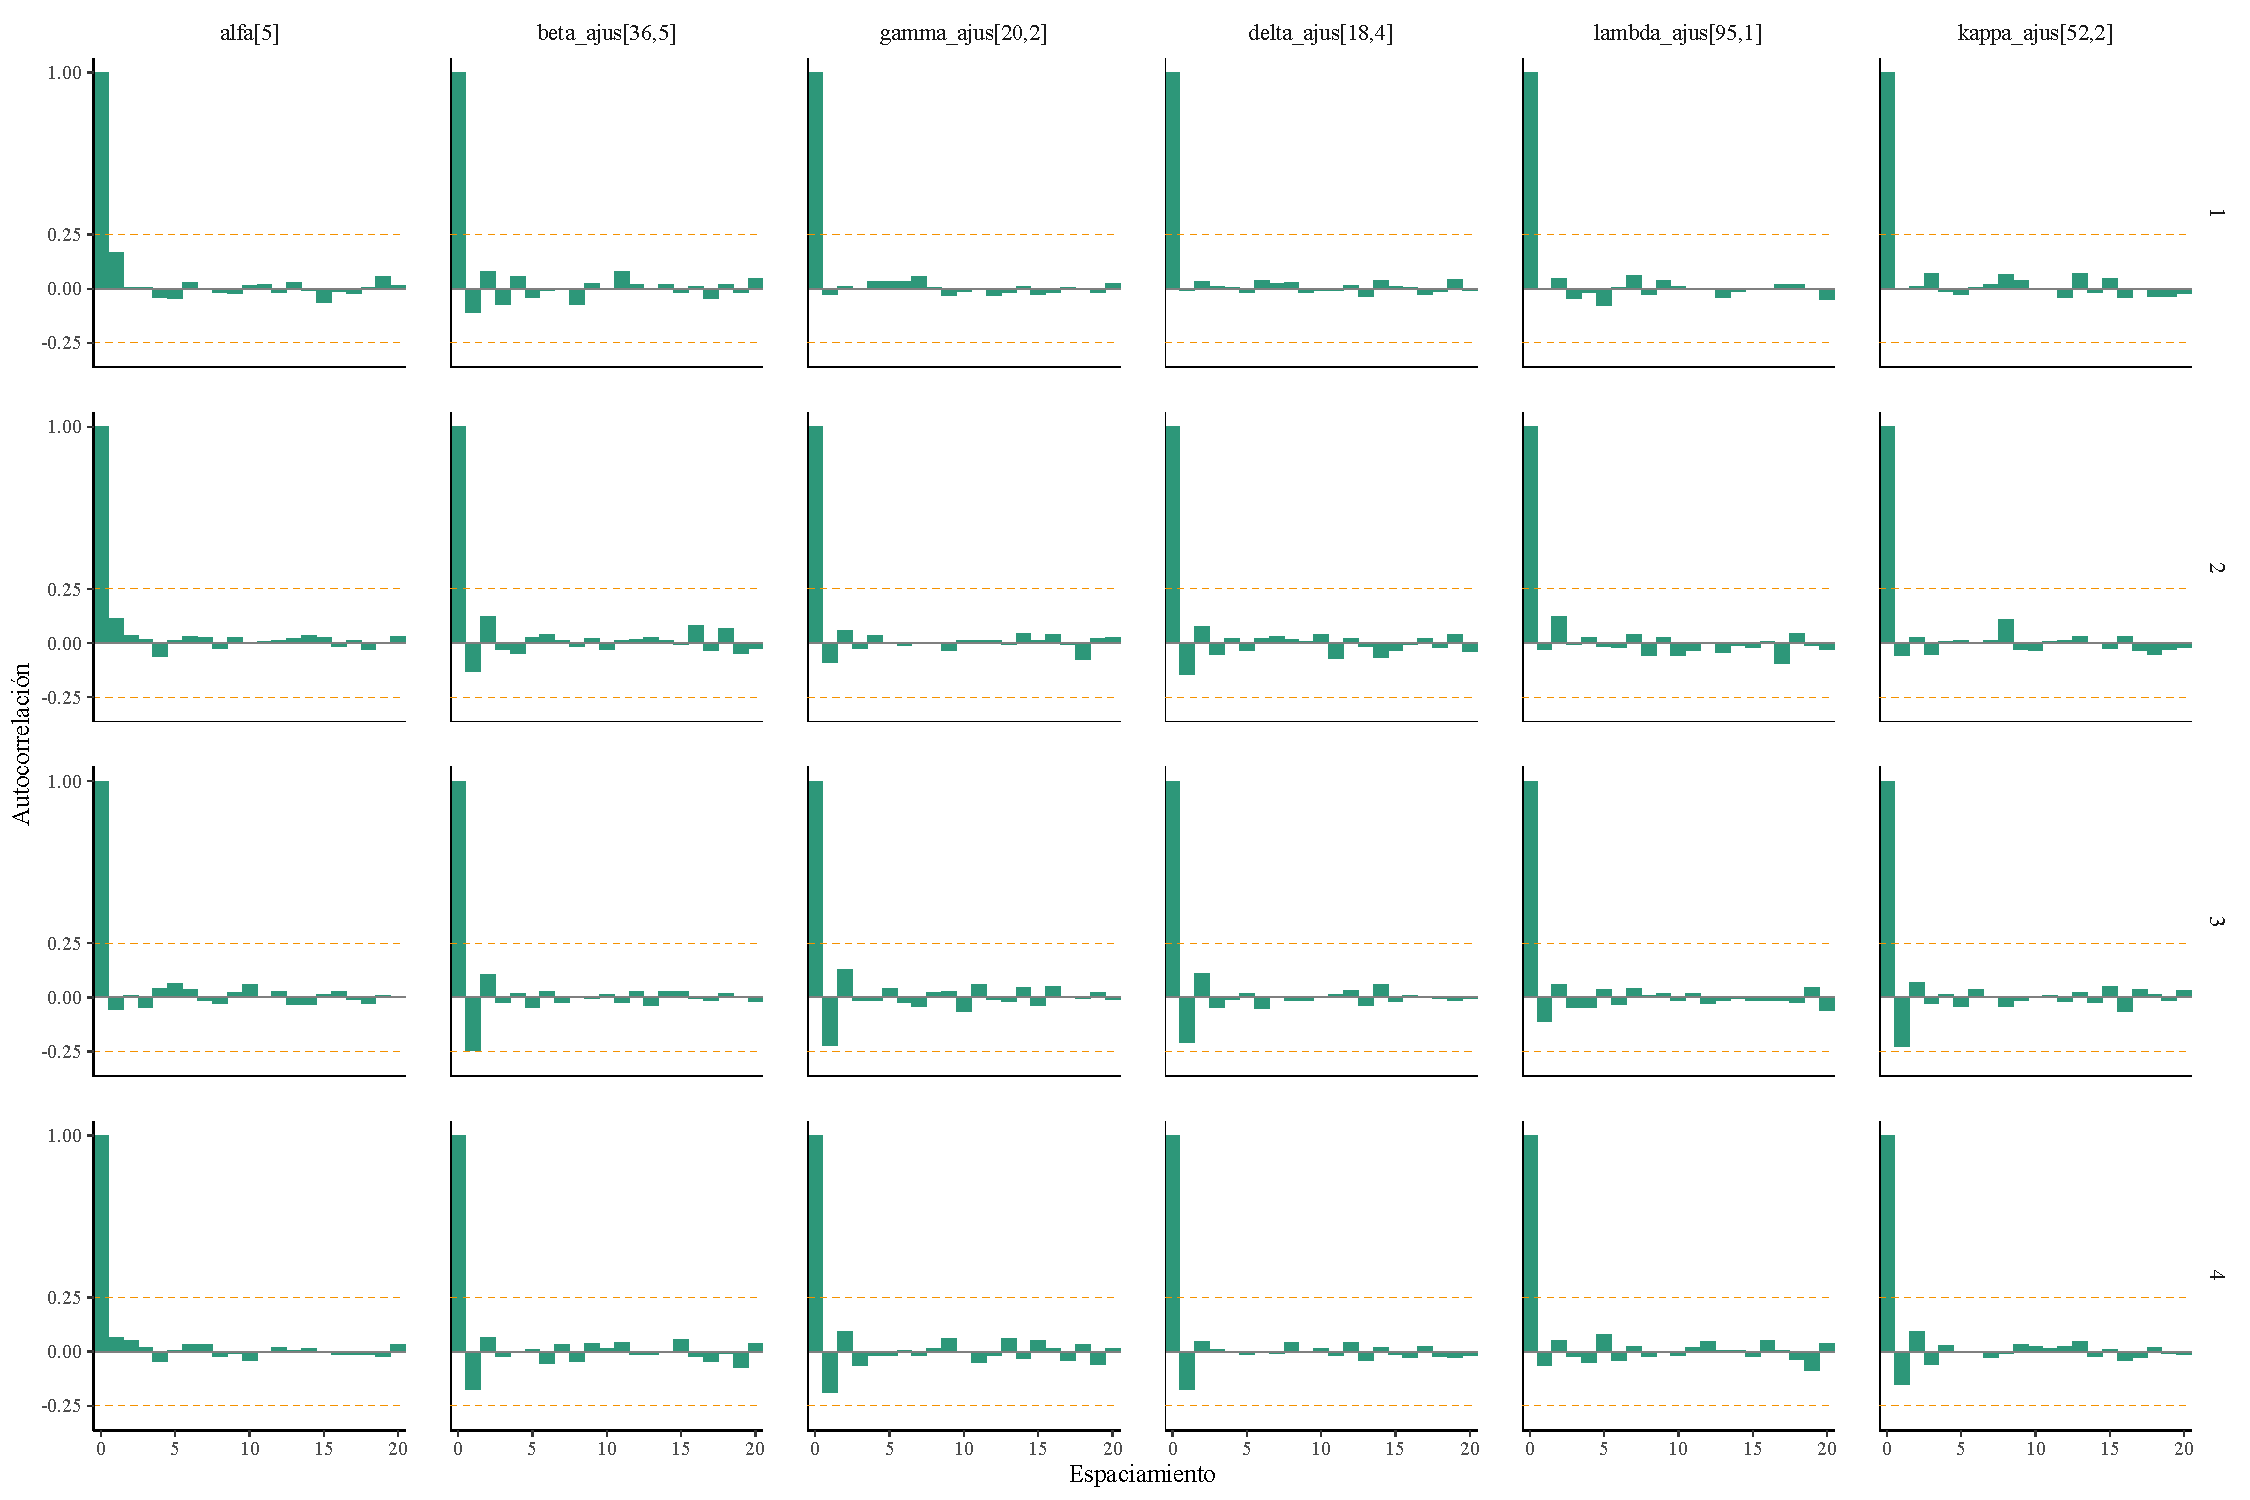
\includegraphics[width = \textwidth]{Figs/Convergencia/Convergencia_AutoCorr}
	\caption{Ejemplo de gráficos de autocorrelación para algunos parámetros del modelo H.}
	\label{fig:Autocorr_H}
	\end{subfigure}
	\caption{Fuente: elaboración propia.}
\end{figure}

 También analicé la convergencia del modelo H mediante los diagnósticos del paquete de $\mathsf{R}$ \textit{shinystan}, que permite de manera interactiva observar distintos gráficos y resúmenes respecto al ajuste del modelo vía HMC. De esta exploración, también concluí que el modelo satisfacía suficientemente bien la batería de diagnósticos para darnos confianza en que las muestras obtenidas provienen de la distribución posterior. Una vez verificada la convergencia, podemos proceder al análisis de los resultados para lo cual debemos interpretar lo que los coeficientes simulados nos dicen. 
 
\section{Efectos de las variables}

Interpretar los coeficientes de regresiones logísticas no es sencillo pues, por la liga logística, estos se encuentran en una escala distinta a la de las proporciones o probabilidades que es en la que normalmente estamos interesados. Como explican \textcite{GelmanHill06}, además de las interpretaciones en términos de momios, una primera alternativa es considerar el caso cuando la variable explicativa vale 1. Sin embargo, esto no siempre tiene sentido dependiendo del contexto en el que se realiza la regresión. Sobre todo para evitar alguna falacia ecológica--- ver página \pageref{No_Extrapolar}--- este es mi caso, por lo que no podría interpretar los coeficientes mediante alguna estrategia de ese tipo.\\ 

 Por ello, resultan útiles lo que los mismos autores llaman \textit{predictive comparisons}. Básicamente estos consisten en pensar en los efectos de los coeficientes en términos de una comparación entre dos valores distintos pero informativos de las variables explicativas de interés; por ejemplo, la media y una desviación estándar por encima de ella. Esta elección tiene la ventaja de que, usualmente, se estaría realizando la interpretación en el rango de valores observado y no mediante una extrapolación. Hay que decir, no obstante, que una situación donde esto puede no suceder es cuando las variables observadas sean multimodales y la media caiga en uno de los valles. Esta discusión general sobre alternativas de interpretación para regresiones logísticas puede consultarse en la referencia antes citada.\\ 
 
\subsection{Definiendo efectos}

 Por nuestra parte, para fijar ideas, recordemos que las variables explicativas son las \textit{configuraciones sociales} definidas por las categorías poblacionales de las variables censales. Supongamos por ahora que estamos analizando un modelo individual nacional para una variable con 3 categorías, $x = (x_1,x_2,x_3)$. Recordando \eqref{eq:Modelo_Nal_Ind} y omitiendo el subíndice de las comunas, tendríamos que para alguna comuna en particular,

\begin{equation*}
ln\left(\dfrac{p}{1-p}\right) = \alpha + \beta_1 x_1 + \beta_2 x_2 + \beta_3 x_3.
\end{equation*}

Abusando de la notación, introduzco ahora unas expresiones. En primer lugar

\begin{equation*}
\eta(x;\beta_i)= \alpha + \beta_i x_i + \sum\limits_{k\neq i} \beta_k x_k, 
\end{equation*} 

para referirme al predictor lineal como función de la configuración social $x$ y considerando el intercepto $\alpha$ y los coeficientes como fijos; pongo énfasis en el coeficiente $\beta_i$ porque es el efecto a interpretar. Asimismo tomemos 

\begin{equation*}
p(x;\beta_i)=\dfrac{e^{\eta(x;\beta_i)}}{1+e^{\eta(x;\beta_i)}}=\dfrac{1}{1+e^{-\eta(x;\beta_i)}}
\end{equation*} 

como el valor de la afinidad por Marine Le Pen en la comuna como función de la configuración social y, de nuevo, con el resto del predictor lineal fijo.\\

 Buscaríamos entonces definir el efecto que tiene el coeficiente $\beta_i$ como el cambio en puntos porcentuales para dicha afinidad cuando se pasa de una configuración a otra. Por ejemplo, suponiendo $x_{(0)}$ como una configuración inicial y $x_{(1)}$ como otra en la que aumenta la categoría de interés, tendríamos que el efecto sería

\begin{equation*}
\Delta(\beta_i;x_{(0)},x_{(1)}) = p(x_{(1)};\beta_i)-p(x_{(0)};\beta_i)
\end{equation*}

Sin embargo, en nuestro caso no tenemos total libertad para elegir los valores $x_{(0)}$ y $x_{(1)}$ pues recordemos que son proporciones que deben sumar a 1. ¿Cómo elegirlos entonces?\\ 

En primer lugar, podemos seleccionar el punto de referencia $x_{(0)}$ como la media muestral, $x_{(0)}=\bar{x}=(\bar{x}_1,\bar{x}_2,\bar{x}_3)$. Posteriormente, como estamos interesados en el efecto del coeficiente $\beta_i$, empecemos a construir $x_{(1)}$ con base en $x_{(1),i}=\bar{x}_i + s_i$ donde $s_i$ es la desviación estándar muestral en la $i$-ésima categoría. Al agregarle una desviación estándar a $x_i$, para cumplir con la restricción, debemos disminuir su valor del resto de las $x_k$ en su conjunto. Sin que sea la única forma de hacerlo, una propuesta es quitarle de manera proporcional a cada categoría restante una parte de la desviación estándar que sumamos a la categoría de interés. Esto sería de la siguiente manera: 

\begin{equation*}
x_{(1),k}=\bar{x}_k - s_i \dfrac{\bar{x}_k}{1-\bar{x}_i} \quad \forall k \neq i
\end{equation*}

Con este criterio podemos abusar un poco más de la notación. Si en lugar del caso específico de una configuración social de 3 categorías tenemos $l$, el efecto sería 

\begin{align*}
\Delta(\beta_i) &= p(x^\star;\beta_i)-p(\bar{x};\beta_i) \quad \forall i \in \mathbb{N}_l \\
\text{donde} \quad \bar{x} &= (\bar{x}_1,\dots,\bar{x}_{l}), \\ 
x_i^\star = \bar{x}_i + s_i \quad &\text{y} \quad x_j^\star =\bar{x}_j - s_i\dfrac{\bar{x}_j}{1- \bar{x}_i} \quad \forall j \neq i 
\end{align*}

La interpretación de los coeficientes sería entonces el efecto predicho en puntos porcentuales al aumentar la proporción de individuos en la categoría de interés respecto a una comuna ``típica''; es decir, al pasar de $\bar{x}$ a $x^\star$.\\ 

Ahora pensemos que querríamos calcular efectos para nuestros modelos jerárquicos. En este caso en lugar de un solo efecto nacional $\Delta(\beta_i)$ tendríamos 96 efectos $\Delta(\beta_{d,i})$, uno para cada departamento. Por lo mismo, simplemente reemplazamos el parámetro de interés por su equivalente jerárquico y tendríamos que calcular la media, $\bar{x}_{d}$, y la desviación estándar correspondiente dentro de cada departamento, $s_{d,i}$: 

\begin{equation*}
\Delta(\beta_{d,i}) =  p(x^\star_{d};\beta_{d,i})-p(\bar{x}_{d};\beta_{d,i}) \quad \forall i \in \mathbb{N}_l
\end{equation*}

¿Pero qué pasa cuando tenemos un modelo compuesto con más de una variable censal? En esta situación, la decisión que tomé fue buscar una comparación \textit{c\ae teris paribus} en la que los sumandos del resto de variables explicativas del predictor lineal toman sus valores promedio en el departamento. Podemos también pensar que estamos modificando el intercepto con los sumandos del resto de categorías con valores promedio. Por ello, si asociamos a $x$ con la variable de la categoría de interés, $\theta$ con sus coeficientes y $z$ con el resto del predictor lineal, una notación más general podría ser

\begin{align}\label{eq:Efecto_Enchufado_Compuesto}
\Delta(\theta_{d,i};\bar{z}_d) &= p(x_d^\star;\theta_{d,i},\bar{z}_d)-p(\bar{x}_d;\theta_{d,i},\bar{z}_d) \quad \forall i \in \mathbb{N}_l \\
\text{donde} \quad p(x_d;\theta_{d,i},\bar{z}_d) &=\dfrac{1}{1+e^{-\eta(x_d;\theta_{d,i},\bar{z}_d)}} \nonumber \\
\text{y} \quad \eta(x_d;\theta_{d,i},\bar{z}_d) &= \bar{z}_d + \theta_{d,i}x_{d,i} + \sum\limits_{k\neq i} \theta_{d,k}x_{d,k}. \nonumber
\end{align}

Por ejemplo, pensemos en el caso del modelo compuesto A que incluye a la escolaridad y a las categorías socioprofesionales. Si queremos el efecto para una categoría de escolaridad, $\theta = \beta$ y este dependería del intercepto y las 8 categorías socioprofesionales vía $\bar{z}_d = \alpha_d + \sum\limits_{j=1}^8 \gamma_{d,k}\bar{x}_{csp,d,k}$. Análogamente, para el efecto de una categoría socioprofesional tendríamos $\theta = \gamma$ y $\bar{z}_d = \alpha_d + \sum\limits_{j=1}^5 \beta_{d,k}\bar{x}_{escol,d,k}$.\\

Hasta aquí ya construimos una propuesta de efecto comparando dos predicciones específicas del modelo ``enchufando'' un valor específico o un estimador puntual de los coeficientes. Sin embargo, tenemos incertidumbre sobre sus valores reflejada mediante muestras posteriores de $S$ valores simulados via HMC. Por lo mismo, siguiendo la única receta de la estadística bayesiana tendríamos que obtener la distribución posterior de los efectos, calculando \eqref{eq:Efecto_Enchufado_Compuesto} para cada simulación posterior $\beta_{d,i}^{(s)}$ y, correspondientemente, $\bar{z}_d^{(s)}$:

\begin{equation*}
\Delta(\beta_{d,i}^{(s)};\bar{z}_d^{(s)}) =  p(x^\star_{d};\beta_{d,i}^{(s)},\bar{z}_d^{(s)})-p(\bar{x}_{d};\beta_{d,i}^{(s)},\bar{z}_d^{(s)}) \quad \forall i \in \mathbb{N}_l ,\, s \in \mathbb{N}_S.
\end{equation*}

Esta sería la distribución posterior de los efectos con la que podemos continuar el análisis de los modelos mediante distintos resúmenes inferenciales como el efecto esperado. Asimismo, podemos resumir la distribución reportando intervalos centrales de probabilidad al 50\%, 90\% y 95\%, así como el efecto mediano. Siguiendo la práctica común, cuando los intervalos centrales al 95\% contienen al 0, diremos que la categoría poblacional no tiene un efecto significativo. Si, por el contrario, se encuentran en su totalidad por encima o por debajo del 0, diremos que se tiene un efecto positivo o negativo, respectivamente. 

\subsection{Escolaridad}


	%\chapter{Conclusiones}

Esta tesis aborda uno de los fenómenos políticos internacionales que, desde mi punto de vista, resulta por de más interesante de estudiar: los movimientos nativistas y autoritarios de corte populista que comúnmente son denominados con etiquetas como derechas radicales o extremas. Un buen punto de partida para estudiar estos movimientos es considerar uno de los partidos más característicos de esta corriente política, el \textit{Front National} francés. Utilizando datos oficiales del censo francés realicé un modelo estadístico de regresión que explicara el voto obtenido por el FN en las elecciones presidenciales del 2012 a partir de las distintas configuraciones sociales que dichos datos definen. Así, este modelo arroja varias lecciones.\\

En primer lugar, debo decir que el análisis estadístico refuerza lo que una parte importante de la literatura revisada sugiere. El clivaje de escolaridad es, probablemente, el más importante o explicativo a la hora de estudiar a estos movimientos NAP. Una mayor presencia a nivel local de personas con escolaridad universitaria o superior inhibió más el voto frontista en 2012 que cualquier otra de las variables consideradas. Por el contrario, una configuración social con mayor presencia de personas sin escolaridad formal o cuyo máximo grado de estudios fue la preparatoria favoreció el voto por la candidata del FN. Me resulta interesante que la variable de escolaridad sea, en este sentido, la más significativa pues es una variable que puede incorporar los dos \textit{resentimientos} que la literatura relacionaría con el fenómeno NAP: el cultural y el económico. La escolaridad tiene consecuencias económicas pero fundamentalmente puedo influir en los valores e ideas que tienen los individuos.\\

En este sentido, podemos conjeturar que ambas explicaciones coexisten pero parecería que la influencia de la ansiedad económica o la consciencia de clase es menor que aquella de la ``cultura política'' entendida como el conjunto de valores sociales e ideología que guía las decisiones políticas de los individuos. La variable socioeconómica por excelencia en los estudios de sociología electoral francesa que rescato de la literatura es la categoría socioprofesional de las personas. A pesar de contribuir a la explicación, parece que la única verdadera clase social--- en el sentido tradicionalmente entendido--- que favoreció el voto frontista fue la clase obrera, confirmando la existencia de un \textit{gaucho-lepensime}. Una mayor presencia de obreros estuvo asociada con un mayor voto frontista aunque, con la excepción de los departamentos de Meuse, Val-de-Marne y Bouches-du-Rhône, en una magnitud menor que los efectos de las categorías de escolaridad. Por el contrario, una configuración social a nivel comuna con mayores niveles de cuadros y profesiones intelectuales inhibió el voto FN en 2012. ¿Existirá una consciencia de clase entre ellos o podemos pensar que el efecto se debe más a su asociación con contextos sociales culturalmente discordantes con el mensaje xenófobo y autoritario del FN?\\ 

Más aún, la influencia que tiene una distinta composición de la población comunal en términos de grupos de edades sería evidencia a favor de teorías culturalistas como las de Inglehart. Las comunas con mayores niveles de jóvenes entre 18 y 24 años tuvieron menor afinidad con Marine Le Pen en la elección presidencial. Las comunas más ``avejentadas'', en el sentido de contar con mayor presencia de personas retiradas o de más de 65 años, también votaron menos por Le Pen. Probablemente esto se deba a que la primera es una generación con valores y preocupaciones distintas a las del FN y, la segunda, la más cercana a la tradición gaullista de la derecha usual. En el sentido opuesto, las comunas con mayores porcentajes de menores de edad reflejaron mayor apoyo al FN. Esto ameritaría un estudio más detallado pero una primera hipótesis podría sugerir una sociedad más rural y también menos cercana a los valores posmodernos de familias pequeñas, mismos que podríamos asociar políticamente a partidos de izquierda como el socialista o el movimiento ecologista. En este mismo espíritu podríamos interpretar la mayoría de efectos negativos asociados a comunas con mayor presencia de mujeres.\\

Ahora bien, contrario a lo que la mayoría de las teorías sobre el conflicto o la competencia fiscal sugerirían que causa la presencia de inmigrantes, este estudio encuentra más bien una relación negativa con el voto frontista. Ello puede deberse a distintos factores. Una mayor cantidad de inmigrantes puede llevar a que más personas de este grupo accedan al derecho al voto, ya sea por naturalización o por un efecto de generaciones siguientes. Estos ciudadanos (pro)inmigrantes tenderían a rechazar el mensaje xenófobo de Le Pen. Adicionalmente, podría ser que la conviviencia a nivel local con inmigrantes elimine el miedo al \textit{Otro} que podría estar alimentando los sentimientos nativistas. Bajo esta hipótesis, más que un conflicto directo entre grupos estaríamos hablando de una xenofobia indirecta y de la ansiedad cultural que asocia la inmigración con un declive de las tradiciones europeas.\\

¿Es el desempleo reflejo de una descomposición económica que favorezca el surgimiento de los movimientos NAP? Hay referencias que particularmente señalan la ansiedad económica causada por el desempleo o fragilidad laboral juvenil. Esta tesis no parece encontrar que estas hipótesis sean las más favorecidas. De hecho, el desempleo juvenil podría considerarse como la variable menos explicativa de todas las aquí consideradas. Si bien observamos que el desempleo en general puede tener un efecto en el voto, este sería más modesto que otros y no en un mismo sentido a nivel nacioanl. En algunos lugares mayor desempleo favoreció el voto frontista y en otros lo inhibió.\\

Esta última consideración me lleva a llamar la atención sobre algo que parecería ser una respuesta frecuente en ciencias sociales y que en ocasiones pasamos por alto: depende. Muchas veces querríamos contar con teorías prístinas y unificantes como la existencia de ``El votante FN'' y sin embargo hay que recordar que la realidad es más compleja. Lo que los modelos de esta tesis señalan es que no existe una única relación entre las variables sociales consideradas. En este sentido estaríamos hablando de diferentes efectos dependiendo del contexto. La posibilidad de llevar a cabo un modelado jerárquico por departamento en lugar de conformarse con un modelo nacional más sencillo nos permite reconocer de mejor manera la variabilidad y la incertidumbre que tenemos sobre estos efectos. Mientras que hay variables con efectos más o menos homogéneos a nivel nacional, existen otras que influyen de manera marcadamente opuesta dependiendo del departamento del que hablemos.

\section*{Trabajo futuro}

Esta tesis, como es de esperarse, más que aportar respuestas definitivas genera nuevas preguntas tanto dentro del análisis de los movimientos NAP como respecto al contexto estadístico. Por lo mismo, señalo algunas de las posibilidades para continuar el estudio así como algunos comentarios respecto del proceso de modelado utilizado.\\

La primera forma de continuar el estudio de los movimientos NAP en general y el FN en particular es ajustar el modelo aquí desarrollado a otras elecciones. Están disponibles los datos para replicar el estudio en la elección del 2007 y, de acuerdo al calendario de difusión de resultados del INSEE, el próximo año contaremos con los datos censales necesarios para aplicarlos a la elección del 2017. El análisis de estas dos elecciones ofrecerían un panorama más completo de las configuraciones sociales del FN pues en la primera el candidato era Le Pen padre y no había pasado la crisis económica de 2008-2009 mientras que en la segunda Marine Le Pen accedió a la segunda vuelta presidencial lo que ofrece la posibilidad de estudiar ambas vueltas electorales. Podría verificarse qué factores han tenido continuidad y cuáles de las variables, de haberlas, han cambiado su efecto. Más aún, podrían también estudiarse las elecciones europeas y legislativas. Estas últimas, sin embargo, tienen la desventaja de no contar con la presencia de candidaturas frontistas en todos los lugares y ser elecciones que podríamos considerar como secundarias por lo que las motivaciones para votar por las diferentes fuerzas políticas suelen ser distintas.\\

Otra ruta es realizar un estudio de política comparada. Hoy por hoy, parecería que la batuta europea de los movimientos NAP la ha tomado la Lega de Matteo Salvini en Italia. El Istat, equivalente al INSEE francés o a nuestro INEGI, también ofrece datos que podrían permitir un estudio comparado de las configuraciones sociales de este partido italiano con aquellas del FN. Asimismo, pueden explorarse comparaciones con otros movimientos NAP. Finalmente, se podrían considerar otras variables además de las aquí utilizadas.\\

Desde el punto de vista estadístico, también existen alternativas para continuar el estudio. Una de las posibles limitaciones de los modelos aquí considerados es que conllevan un alto costo computacional por lo que tuvo que seleccionarse una muestra de comunas. Con menores restricciones de tiempo y/o mayor poder de cómputo podrían considerarse más datos o modelos distintos. Por ejemplo, el modelado jerárquico permite naturalmente la incorporación de variables a distintos niveles de agregación. En este sentido es posible modificar el modelo para incorporar información tanto a nivel comunal como a nivel departamental.\\ 

Otras tres familias de modelos que aquí no se consideraron pero que para trabajos futuros podrían resultar de interés serían los modelos espaciales para incorporar relaciones de cercanía geográfica, los modelos dinámicos en caso de realizar comparaciones temporales y los modelos sobredispersos para poder modelar de mejor manera la variabilidad de datos discretos como el número de votos. Adicionalmente, puedo decir que el uso de datos censales agregados ofrece la posibilidad de contar con datos de una mayor cobertura geográfica pero sacrifica la inferencia a nivel individual en el camino. En este tenor una línea de investigación atractiva sería la inferencia ecológica que busca superar el obstáculo de no poder ofrecer inferencias individuales con base en datos con niveles mayores de agregación.\\

Finalmente, quisiera comentar que otro de los propósitos de esta tesis fue discutir y aplicar el paradigma estadístico bayesiano que tuve la oportunidad de conocer mediante materias optativas durante la carrera. Mi tesis busca presentar una introducción a este paradigma pues considero que ofrece grandes posibilidades para las ciencias sociales. Por lo mismo, espero contribuir a su difusión ejemplificando una aplicación a un problema proveniente de una ciencia social. Al mismo tiempo, aproveché para explorar el método de \textit{Hamiltonian Monte Carlo} implementado mediante Stan, que podría considerarse como un \textit{software} a la vanguardia de la aplicación práctica de la inferencia bayesiana. Sin embargo, considerando las limitaciones de tiempo podemos preguntarnos si existen alternativas más eficientes que permitan una buena inferencia bayesiana. Métodos como inferencia variacional o INLA podrían representar este papel.\\

No quisiera terminar este trabajo sin reafirmar mi convicción de que la dignidad humana es sagrada. Por ello, busqué estudiar una corriente ideológica que, desde mi particular punto de vista, atenta constantemente contra ella. No es sino intentando entender por qué, cómo y dónde surgen estos movimientos que podremos dar respuestas y mitigar las consecuencias dañinas que de ellos se deriven. Es natural tener miedo por el futuro, pero deseo firmemente que quienes por distintas circunstancias lo experimenten, puedan encontrar esperanza sin odio a otros seres humanos.
 
 



%%%%%%%%%%%%%%%%%%%%%%%%%%%%%%%%%%%%%%%%%%%%%%%%%%%%%%%%%%%%%
%%  ANEXOS %%%
%%%%%%%%%%%%%%%%%%%%%%%%%%%%%%%%%%%%%%%%%%%%%%%%%%%%%%%%%%%%%
\appendix

\addcontentsline{toc}{part}{Anexos}
\part*{Anexos}
\chapter{Análisis bayesiano del modelo lineal normal}\label{Anexo_modelo_lineal}

Para realizar un análisis bayesiano del modelo lineal normal requerimos especificar una distribución inicial para $\theta$ y, mediante el teorema de Bayes, actualizarla para obtener una distribución posterior dados los datos observados. Entonces, primero presento una manipulación de la función de verosimilitud para después ver algunas distribuciones iniciales frecuentemente utilizadas y, finalmente, realizar la actualización de las mismas dados los datos. 

\subsubsection*{Verosimilitud}

Siguiendo a \textcites{GP98}{Congdon06}, manipulemos la función de verosimilitud de la normal multivariada para facilitar la actualización mediante el teorema de Bayes. Observemos que:
\begin{align}\label{eq:modelo_normal_prop}
f(y|\theta) &= \dfrac{1}{\sqrt{(2\pi)|\sigma^2 \mathbb{I}_N|}}exp\left\lbrace -\dfrac{1}{2}(y-X\beta)^T(\sigma^2\mathbb{I}_N)^{-1}(y-X\beta)\right\rbrace \nonumber \\
 &\propto (\sigma^2)^{-n/2}exp\left\lbrace -\dfrac{1}{2\sigma^2}(y-X\beta)^T(y-X\beta)\right\rbrace
\end{align}

En el análisis clásico o frecuentista, el estimador máximo verosímil para los coeficientes $\beta$ es $b=(X^TX)^{-1}X^Ty$. Podemos manipular los términos dentro de la exponencial en la distribución normal con este estimador $b$: 
\begin{align} \label{eq:producto_exponente_normal}
y-X\beta &= y - Xb + Xb - X\beta = (y-Xb) + X(b-\beta) \nonumber \\
\Rightarrow (y-X\beta)^T(y-X\beta) &= \left\lbrace (y-X\beta)^T + \left[X(b-\beta)\right]^T \right\rbrace \Big\{ (y-Xb) + X(b-\beta) \Big\} \nonumber \\
 & = (y-Xb)^T(y-Xb) + (y-Xb)^TX(b-\beta) + \nonumber \\
 &\qquad \left[X(b-\beta)\right]^T(y-Xb) + \left[X(b-\beta)\right]^TX(b-\beta) \nonumber \\
\intertext{y, agrupando los términos cruzados en $k(y,\beta)$,}
\Rightarrow (y-X\beta)^T(y-X\beta) & = (y-Xb)^T(y-Xb) + (b-\beta)^TX^TX(b-\beta) + k(y,\beta)\,.
\end{align}
En realidad, $k(y,\beta) = 0$: 
\begin{align*}
k(y,\beta) &= (y-Xb)^TX(b-\beta) + \left[X(b-\beta)\right]^T(y-Xb)
\intertext{notando que el segundo término es igual al primero pero transpuesto,}
(y-Xb)^TX(b-\beta) &= (y^T - b^TX^T)(Xb-X\beta)
\intertext{sustituyendo el valor de $b$ y considerando que $Xb=y$}
(y-Xb)^TX(b-\beta) &= 
\Big\{ y^T - \left[(X^TX)^{-1}X^Ty \right]^TX^T \Big\}
(y-X\beta) \\
 &= \Big\{y^T - \left[y^TX(X^TX)^{-T}\right]X^T\Big\}
 (y-X\beta)\\
 &= \left[y^T - y^TX(X^{-1}X^{-T})X^T\right]
 (y-X\beta)\\
 &= (y^T - y^T)(y-X\beta)
\intertext{entonces,}
(y-Xb)^TX(b-\beta) &= 0 \quad \Longrightarrow \quad k(y,\beta) = 0\,.
\end{align*}
Podemos entonces sustituir \eqref{eq:producto_exponente_normal} con $k(y,X,\beta) = 0$ en \eqref{eq:modelo_normal_prop}: 
\begin{align*}
f(y|\theta) &\propto (\sigma^2)^{-n/2}exp\left\lbrace -\dfrac{1}{2\sigma^2}\left[(y-Xb)^T(y-Xb) + (b-\beta)^TX^TX(b-\beta)\right] \right\rbrace\\
&\propto (\sigma^2)^{-n/2}exp\left\lbrace -\dfrac{1}{2\sigma^2}\left[(y-Xb)^T(y-Xb) + (\beta-b)^TX^TX(\beta-b)\right] \right\rbrace
\end{align*}
Igual que con el estimador $b$ para los coeficientes, podemos utilizar el estimador máximo verosimil de la varianza, $\hat{\sigma}^2=\dfrac{1}{N}(y-Xb)^T(y-Xb)$, para preparar la verosimilitud de $y|\theta$:
\begin{equation*}
f(y|\theta) \propto (\sigma^2)^{-n/2}exp\left\lbrace -\dfrac{1}{2\sigma^2}\left[N\hat{\sigma}^2 + (\beta-b)^TX^TX(\beta-b)\right] \right\rbrace
\end{equation*}
Notemos ahora que si la varianza $\sigma^2$ fuera conocida podríamos descomponer esta distribución en dos partes, una de las cuales tiene la forma del kernel de una distribución normal para $\beta|\sigma^2$, lo que sugiere ya la familia conjugada de distribuciones iniciales:
\begin{equation*}
f(y|\theta) \propto exp\left\lbrace -\dfrac{1}{2\sigma^2}\left[(\beta-b)^TX^TX(\beta-b)\right] \right\rbrace (\sigma^2)^{-N/2} exp\left\lbrace -\dfrac{N\hat{\sigma}^2}{2\sigma^2}\right\rbrace \,.
\end{equation*}
Finalmente, en este contexto resultará más fácil trabajar en términos de precisiones que de varianzas. Si definimos la precisión de una variable normal como $\tau=\dfrac{1}{\sigma^2}$, tenemos que la función de verosimilitud en el modelo normal se puede representar como sigue: 
\begin{equation} \label{eq:verosimilitud_modelo_normal}
p(y|\theta) \propto exp\left\lbrace -\dfrac{\tau}{2}\left[(\beta-b)^TX^TX(\beta-b)\right] \right\rbrace \tau^{N/2}exp\left\lbrace -\dfrac{N\hat{\sigma}^2\tau}{2}\right\rbrace \,.
\end{equation}

\subsubsection*{Distribuciones iniciales}

La primera distribución inicial que podríamos plantear sería la distribución conjugada. Recordemos que esta debe tener la misma forma funcional que la verosimilitud, por lo que \eqref{eq:verosimilitud_modelo_normal} sugiere lo siguiente: 
\begin{equation*}
f(\theta)= f(\beta,\tau) \propto exp\left\lbrace -\dfrac{\tau}{2}\left[(\beta-b_0)^TT_0(\beta-b_0)\right] \right\rbrace \tau^{a/2} exp\left\lbrace -\dfrac{r\tau}{2}\right\rbrace \,,
\end{equation*}
donde $b_0$, $T_0$, $a$ y $r$ sean algunos parámetros convenientes. Con esta forma, podemos determinar la familia conjugada en un proceso de dos pasos. En primer lugar, asumimos que la varianza o precisión está dada, lo que permite definir una distribución inicial para $\beta|\tau$. Posteriormente, determinaremos la distribución inicial conjugada para $\tau$. Es decir, separaremos la distribución inicial en dos: $f(\theta)=f(\beta,\tau)=f(\beta|\tau)f(\tau)$.\\ 

La distribución condicional resulta ser una normal centrada en $b_0$ y con precisión $\tau T_0$, por lo que debemos completarla multiplicando por $1=\tau^{(d-d)/2}$, donde $d$ es el número de coeficientes, incluyendo a $\beta_0$. Así: 
\begin{align} \label{eq:distr_ng}
f(\theta)= f(\beta|\tau)f(\tau) &\propto exp\left\lbrace -\dfrac{\tau}{2}\left[(\beta-b_0)^TT_0(\beta-b_0)\right] \right\rbrace \tau^{a/2} exp\left\lbrace -\dfrac{r\tau}{2}\right\rbrace \nonumber \\
&\propto \tau^{(d - d)/2} exp\left\lbrace -\dfrac{\tau}{2}\left[(\beta-b_0)^TT_0(\beta-b_0)\right] \right\rbrace \tau^{a/2} exp\left\lbrace -\dfrac{r\tau}{2}\right\rbrace \,. \nonumber\\
\intertext{Con lo que} \nonumber 
f(\beta|\tau) &\propto \tau^{d/2} exp\left\lbrace -\dfrac{\tau}{2}\left[(\beta-b_0)^TT_0(\beta-b_0)\right] \right\rbrace \,\text{y} \nonumber \\
f(\tau) &\propto \tau^{(a-d)/2} exp\left\lbrace -\dfrac{r\tau}{2}\right\rbrace \,.
\end{align}

La distribución inicial de $\tau$ también ya tiene una forma conocida: es proporcional a una gamma. Para verlo solo basta con un poco de álgebra para verificar que el parámetro de forma debe ser $a_0 = (a-d+2)/2=(a^\star-d)/2$ con $a^\star=a+2$ y el de tasa $r_0 = r/2$. Por lo tanto, en su conjunto, tenemos que $\theta$ tiene una distribución inicial \textit{Normal-Gamma}: 
\begin{align} 
\theta &= (\beta,\tau) \sim NG_d\left(b_0,T_0,a_0=\dfrac{a^\star-d}{2},r_0 =\dfrac{r}{2}\right) \nonumber \\
\intertext{de forma que}
\beta|\tau &\sim N_d(b_0,\tau T_0) \;\text{y}\; \tau \sim \Gamma\left(a_0 = \dfrac{a^\star-d}{2}, r_0 = \dfrac{r}{2}\right) \,.
\label{eq:normal_gamma}
\end{align}
Cabe hacer notar que esta distribución inicial conjugada es propia siempre que $a^\star > d $, $r > 0$ y $B_0 = T_0^{-1}$ sea positiva definida.\\ 

Por otro lado, si se buscan distribuciones iniciales más vagas, resulta que también es posible obtener distribuciones mínimo informativas límites de esta conjugada. Por ejemplo, aunque es impropia, la inicial de Jeffreys es de esa forma con los siguientes límites: $a^\star \rightarrow d $, $r \rightarrow 0$ y $B_0 = T_0^{-1} \rightarrow \mathbf{O}$. La \eqref{eq:distr_ng} se reduce a la siguiente expresión \parencite{GP98}: 
\begin{equation} \label{eq:jeffreys_ng}
f(\theta) = f(\beta,\tau) \propto \tau^{(d-2)/2}
\end{equation}

\subsubsection*{Distribuciones finales}

Consideremos para la actualización el caso general de la distribución inicial normal gamma de \eqref{eq:normal_gamma}. 
\begin{align} \label{eq:modelo_normal_pre_bayes}
y|\theta &\sim N_N(X\beta,\sigma^2\mathbb{I}_N) \quad \text{tal que} \quad \theta = (\beta, \sigma^2) \sim f(\beta,\sigma^2) \nonumber \\
\beta|\tau &\sim N_d(b_0,\tau T_0) \nonumber \\ 
\tau &\sim \Gamma\left(a_0 = \dfrac{a^\star-d}{2},r_0 = \dfrac{r}{2}\right) \,.
\end{align}

Aplicaremos el teorema de Bayes con base en \eqref{eq:verosimilitud_modelo_normal} y \eqref{eq:distr_ng} buscando, al tener una inicial conjugada, mantener la forma de normal gamma. Esto es, la verosimilitud la podemos ver también como el producto de dos distribuciones, una normal para $\beta|\tau$ centrada en el estimador máximo verosímil $b$ y con precisión $\tau X^TX$ y una gamma para $\tau$ utilizando el estimador máximo verosímil de la varianza $\hat{\sigma}^2$. 
\begin{align} \label{eq:post_normal_gamma_todo}
f(\theta|y) &\propto f(y|\theta)f(\theta)\nonumber \\
&\propto exp\left\lbrace -\dfrac{\tau}{2}\left[(\beta-b)^TX^TX(\beta-b)\right] \right\rbrace \tau^{N/2} exp\left\lbrace -\dfrac{N\hat{\sigma}^2\tau}{2}\right\rbrace \nonumber \\
&\qquad  \tau^{d/2} exp\left\lbrace -\dfrac{\tau}{2}\left[(\beta-b_0)^TT_0(\beta-b_0)\right] \right\rbrace \tau^{(a-d)/2} exp\left\lbrace -\dfrac{r\tau}{2}\right\rbrace \nonumber \\
&\propto \tau^{d/2} exp\left\lbrace -\dfrac{\tau}{2}\left[(\beta-b)^TX^TX(\beta-b) + (\beta-b_0)^TT_0(\beta-b_0)\right]\right\rbrace \nonumber \\
& \qquad \tau^{(N - d + a)/2} exp\left\lbrace -\dfrac{N\hat{\sigma}^2 + r}{2}\tau\right\rbrace \,.
\end{align}
Ahora simplifiquemos el término dentro de la primera exponencial para que coincida con el kernel de una distribución normal. 
\begin{align} \label{eq:termino_exp_post_normal_gamma}
&(\beta - b)^T X^TX (\beta-b) + (\beta - b_0)^T T_0 (\beta-b_0) \nonumber \\
&\; = \beta^TX^TX\beta - \beta^TX^TXb - b^TX^TX\beta + b^TX^TXb \,+ \nonumber \\ 
&\qquad \beta^TT_0\beta - \beta^TT_0b_0 - b_0^TT_0\beta + b_0^TT_0b_0  \nonumber \\
\intertext{notando que todos estos términos son escalares de forma que sus transpuestos son ellos mismos, así como que $T_0^T=T_0$,}\nonumber 
&\; = \beta^TX^TX\beta - 2\beta^TX^TXb + b^TX^TXb + \beta^TT_0\beta - 2\beta^TT_0b_0 + b_0^TT_0b_0 \nonumber \\
&\; = \beta^T(X^TX + T_0)\beta - 2\beta^TX^TXb - 2\beta^TT_0b_0 + b^TX^TXb + b_0^TT_0b_0 \nonumber \\
\intertext{definiendo $T_1=X^TX + T_0 \quad$ y $\quad g(X,y)=b^TX^TXb + b_0^TT_0b_0$,} \nonumber 
&\; = \beta^TT_1\beta - 2\beta^TX^TXb - 2\beta^TT_0b_0 + g(X,y) \nonumber \\
&\; = \beta^TT_1\beta - 2\beta^T\left[X^TXb + T_0b_0\right] + g(X,y) \nonumber \\
\intertext{definiendo $b_1=T_1^{-1}(X^TXb+T_0b_0)$ y completando el cuadrado:} \nonumber
&\; = \beta^TT_1\beta - 2\beta^TT_1b_1 + g(X,y) \nonumber \\
&\; = (\beta-b1)^TT_1(\beta-b_1) + g(X,y) - b_1^TT_1b_1 \,.
\end{align}
Con esta manipulación de términos, ya podemos tener la distribución posterior de $\beta|\tau$, sustituyendo \eqref{eq:termino_exp_post_normal_gamma} en \eqref{eq:post_normal_gamma_todo}, como una normal $d$-variada con media $b_1$ y precisión $\tau T_1$: 
\begin{align*}
f(\theta|y) &\propto \tau^{d/2} exp\left\lbrace -\dfrac{\tau}{2}\left[(\beta-b1)^TT_1(\beta-b_1)\right]\right\rbrace \\
& \qquad \tau^{(N - d + a)/2} exp\left\lbrace -\dfrac{N\hat{\sigma}^2 + g(X,y) - b_1^TT_1b_1 + r}{2}\tau\right\rbrace \,.
\end{align*}
La nueva media $b_1=T_1^{-1}(X^TXb+T_0b_0)$ puede verse como un promedio de las medias originales--- la de la inicial y el estimador máximo verosímil--- ponderadas por sus precisiones \parencite{Congdon06}. La nueva precisión es simplemente la suma de las precisiones originales.\\

Ahora debemos encontrar los nuevos parámetros de forma y tasa para la distribución posterior de $\tau$. Igualando el exponente de $\tau$ en la última expresión a $a_1-1$, donde $a_1$ es el nuevo parámetro de forma, para satisfacer la representación de una distribución gamma se llega a que $a_1=(N-d+a^\star)/2$. El nuevo parámetro de tasa $r_1$ requiere ser un poco más explícitos: 
\begin{align*}
r_1 &= \dfrac{N\hat{\sigma}^2 + g(X,y) - b_1^TT_1b_1 + r}{2} \\
&= \dfrac{(y-Xb)^T(y-Xb) + b^TX^TXb + b_0^TT_0b_0 - b_1^TT_1b_1 + r}{2} \,.
\end{align*}
Pero resulta que $(y-Xb)^T(y-Xb) + b^TX^TXb = y^Ty$: 
\begin{align} \label{eq:aux_para_jeffreys_ng}
(y-Xb)^T(y-Xb) + b^TX^TXb &= y^Ty - 2y^TXb + b^TX^TXb + b^TX^TXb \nonumber \\
&= y^Ty - 2y^TXb + 2b^TX^TXb \nonumber \\
&= y^Ty - 2b^TX^TXb + 2b^TX^TXb \nonumber \\
&= y^Ty \,.
\end{align}
Por lo que, en realidad, 
\begin{equation*}
r_1 = \dfrac{y^Ty + b_0^TT_0b_0 - b_1^TT_1b_1 + r}{2} \,.
\end{equation*}
Con esto tenemos que la actualización de las \eqref{eq:modelo_normal_pre_bayes} nos llevan al siguiente modelo conjugado: 
\begin{align} \label{eq:modelo_normal_post_bayes}
y|\theta &\sim N_N(X\beta,\sigma^2\mathbb{I}_N) \quad \text{tal que} \quad \theta = (\beta, \sigma^2) \sim f(\beta,\sigma^2) \nonumber \\
\beta|\tau &\sim N_d(b_0,\tau T_0) \qquad  \tau \sim \Gamma\left(a_0 = \dfrac{a^\star-p}{2},r_0 = \dfrac{r}{2}\right) \nonumber \\ 
\beta|\tau , y &\sim N_p(b_1,\tau T_1) \qquad \tau|y \sim \Gamma\left(a_1,r_1\right) \nonumber \\
\intertext{con $a^\star > d $, $r > 0$ y $B_0 = T_0^{-1}$ positiva definida y tal que} \nonumber
T_1 &= X^TX+T_0 \qquad b_1 = T_1^{-1}(X^TXb+T_0b_0) = T_1^{-1}(X^Ty+T_0b_0),\nonumber \\ 
a_1 &= \dfrac{N-d+a^\star}{2} \qquad r_1 = \dfrac{y^Ty + b_0^TT_0b_0 - b_1^TT_1b_1 + r}{2}
\end{align}
donde $b=(X^TX)^{-1}X^Ty$ es el estimador máximo verosímil de $\beta$. Más aún, si en lugar de utilizar como distribución inicial una normal gamma de esta forma se utiliza la inicial de Jeffreys de \eqref{eq:jeffreys_ng}, podemos utilizar estas expresiones para hacer la actualización--- aprovechando el carácter que la inicial de Jeffreys tiene como límite de conjugadas--- considerando $a^\star \rightarrow d $, $r \rightarrow 0$ y $B_0 = T_0^{-1} \rightarrow \mathbf{O}$, por lo que se tendrían: 
\begin{equation*}
T_1 = X^TX \qquad b1 = b \qquad a_1 = \dfrac{N}{2} \qquad r_1 = \dfrac{y^Ty - b^TX^TXb}{2}=\dfrac{N\hat{\sigma}^2}{2} \,
\end{equation*}
donde la equivalencia del estimador máximo verosímil $\hat{\sigma}^2$ puede verificarse con \eqref{eq:aux_para_jeffreys_ng}.\\


%\chapter{Bases de datos utilizadas}

Resultados electorales completos: 

La prelimpieza de estas bases solo consistió en eliminar los códigos al inicio de los archivos de texto. Todos tienen el mismo esquema de nombre original $EEaa\_Bvot\_T1T2$ donde EE es LG para legislativas y PR para presidenciales y los años son 07 y 12. Las bases alteradas tienen el sufijo FAZH, separado por guión bajo. 
\begin{enumerate}
\item Presidenciales 2007 \parencite{PresFr07}
\item Legislativas 2007 \parencite{LegisFr07}
\item Presidenciales 2012 \parencite{PresFr12}
\item Legislativas 2012 \parencite{LegisFr12}
\end{enumerate}

Hasta el momento tengo las siguientes bases de datos: 

\begin{itemize}
\item \textbf{Datos censales}, a nivel comuna que incluyen 3 grupos de edad comparables, 2 categorías de situación migratoria, 2 categorías de nacionalidad, sexo, 6 categorías de tipo de actividad y 8 categorías socioprofesionales. 
\begin{enumerate}
\item IMG1 2007
\item NAT3A 2007
\item IMG2A 2012
\item NAT3A 2012
\end{enumerate}
\item \textbf{Datos de escolaridad}, a nivel comuna y que incluyen grupos de edad y por sexo para personas escolarizadas y no escolarizadas. De las no escolarizadas se tiene el grado más elevado alcanzado, 7 categorías.
\begin{enumerate}
\item Diplômes-Formation 2007
\item Diplômes-Formation 2012
\end{enumerate}
\item \textbf{Datos económicos}, a nivel (algunas) comuna, departamento y región.
\begin{enumerate}
\item Algunos datos de distribución de ingresos por comunas, con secreto estadístico
\item Distribución del ingreso y Gini por dpto.
\item PIB real por región.
\end{enumerate} 
\item \textbf{Datos delictivos}, a nivel departamento, casos por diferentes tipos de delitos (víctimas, procedimientos, instancias, agresores)
\begin{enumerate}
\item Datos mensuales 1996-2017
\end{enumerate}
\end{itemize}

Sin embargo tengo algunas dudas: 

\begin{enumerate}
\item ¿Cómo mezclar los datos delictivos con diferentes unidades de medición? 
\item Hice una sublista de delitos que consideré poco relevantes, para excluirlos del análisis. 
\item Dado que los datos delictivos son mensuales, ¿debería usar datos del año de la elección o de los 12 meses anteriores a la elección?
\item Los datos económicos tuvieron algunos cambios entre los periodos de análisis. Para datos de distribución de ingreso y Gini se pueden hacer comparaciones entre 2006 y 2011, pero no de 2007 a 2012. Para datos del PIB cambió la forma de medirlo en 2008. 
\item En general, ¿combiene usar niveles o cambios?
\item Para el AED, ¿presento variable por variable o de una vez cruces?
\end{enumerate}

\begin{itemize}
\item Para delitos, tasas por cada 100,000 hab en tres categorías (baja, media, alta) y caja y brazos. 
\item Si tiene que ser proporciones. Puede ser modelo binomial para cada partido con n el listado nominal. Normal para el logit de las prop desplazadas. 
\end{itemize}

\begin{table}
\centering
\begin{tabular}{l c c c}
\textbf{Variable} & \textbf{Tipo} & \textbf{2007} & \textbf{2012} \\
\hline 
Vuelta & C & $\diamond$ & $\diamond$  \\
Código de departamento & C & $\diamond$ & $\diamond$  \\
Código de comuna & C & $\diamond$ & $\diamond$  \\
Nombre de comuna & C & $\diamond$ & $\diamond$  \\
Circunscripción legislativa & C &  & $\diamond$  \\
Número de cantón & C &  & $\diamond$  \\
Número de casilla & C & $\diamond$ & $\diamond$  \\
Inscritos & N & $\diamond$ & $\diamond$  \\
Votantes & N & $\diamond$ & $\diamond$  \\
Votos expresados & N & $\diamond$ & $\diamond$  \\
Número de candidatura & C & $\diamond$ & $\diamond$  \\
Apellido de candidato(a) & C & $\diamond$ & $\diamond$  \\
Nombre(s) de candidato(a) & C & $\diamond$ & $\diamond$  \\
Etiqueta política & C & $\diamond$ & $\diamond$  \\
Votos para la candidatura  & N & $\diamond$ & $\diamond$  \\
\end{tabular}
\caption{Descripción de variables en las bases de resultados electorales a nivel casilla para las elecciones presidenciales y legislativas de 2007 y 2012. Los tipos de variables son categóricas (C) o numéricas (N). El diamante indica que la variable está presente en las bases correspondientes. Fuente: elaboración propia.}
\label{tbl:Bases_electorales}
\end{table}


\begin{table}
\centering
\resizebox{\linewidth}{!}{
\begin{tabular}{l *{5}{c}}
\textbf{Variable} & \textbf{Tipo} 
& \textbf{IMG1A 2007} 
& \textbf{IMG2A 2012} 
& \textbf{NAT3A 2007}
& \textbf{NAT3A 2012}\\
\hline 
Nivel & C & $\diamond$ & $\diamond$ & $\diamond$ & $\diamond$  \\
CODGEO & C & $\diamond$ & $\diamond$ & $\diamond$ & $\diamond$  \\
LIBGEO & C &  & $\diamond$ & & $\diamond$ \\
Sexo & C & $\diamond$ & $\diamond$  & $\diamond$ & $\diamond$\\
Edad 4 & C & $\diamond$ &  &  & \\
Edad 4A & C &  & $\diamond$ &  &  \\
Tipo de actividad & C & $\diamond$ & $\diamond$ &  &  \\
Categoría socioprofesional & C &  &  & $\diamond$ & $\diamond$ \\
Condición migratoria & C & $\diamond$ & $\diamond$ &  &  \\
Nacionalidad & C &  &  & $\diamond$ & $\diamond$  \\
Número de personas & N & $\diamond$ & $\diamond$ & $\diamond$ & $\diamond$ \\
\end{tabular}
}
\caption{Descripción de variables en las bases censales a nivel comuna sobre migración y nacionalidad. Los tipos de variables son categóricas (C) o numéricas (N). El diamante indica que la variable está presente en la base correspondiente. Fuente: elaboración propia.}
\label{tbl:Bases_censales}
\end{table}

\begin{table}
\centering
\resizebox{\linewidth}{!}{
\begin{tabular}{l *{4}{c}}
\textbf{Variable} 
& \textbf{Datos administrativos}
& \textbf{Totales} 
& \textbf{Escolarizados} 
& \textbf{No Escolarizados de 15 años o más}\\
\hline 
CODGEO & $\diamond$ & $\diamond$ & $\diamond$ & $\diamond$\\
Código de Región & $\diamond$ & & & \\
Código de Departamento & $\diamond$ & & & \\
LIBGEO & $\diamond$ & & & \\
Sexo & & $\diamond$ & $\diamond$  & $\diamond$ \\
Edad 7 & & $\diamond$ & $\diamond$ & \\
Grado máximo de estudios & & & & $\diamond$ \\
\end{tabular}
}
\caption{Descripción de variables en las subbases a nivel comuna sobre escolaridad. El diamante indica que la variable está presente en la subbase correspondiente. Todas las variables son las mismas para 2007 y para 2012. Fuente: elaboración propia.}
\label{tbl:Bases_escolaridad}
\end{table}

\begin{table}
\centering
\resizebox{\linewidth}{!}{
\begin{tabular}{l *{4}{c}}
\textbf{Variable} 
& \textbf{Datos administrativos}
& \textbf{Totales} 
& \textbf{Escolarizados} 
& \textbf{No Escolarizados de 15 años o más}\\
\hline 
CODGEO & $\diamond$ & $\diamond$ & $\diamond$ & $\diamond$\\
Código de Región & $\diamond$ & & & \\
Código de Departamento & $\diamond$ & & & \\
LIBGEO & $\diamond$ & & & \\
Sexo & & $\diamond$ & $\diamond$  & $\diamond$ \\
Edad 7 & & $\diamond$ & $\diamond$ & \\
Grado máximo de estudios & & & & $\diamond$ \\
\end{tabular}
}
\caption{Descripción de variables en las subbases a nivel comuna sobre escolaridad. El diamante indica que la variable está presente en la subbase correspondiente. Todas las variables son las mismas para 2007 y para 2012. Fuente: elaboración propia.}
\label{tbl:Bases_escolaridad}
\end{table}
%\chapter{Análisis exploratorio de datos complementario}

En este anexo se presentan resúmenes tabulados y gráficos de los datos utilizados y las elecciones consideradas con el objetivo de complementar, para el lector interesado, el análisis exploratorio de los datos. 

\section*{Resultados generales de las 4 elecciones}

En esta sección presento unas tablas de resumen de los resultados electorales oficiales del Ministerio del Interior francés para las 4 elecciones consideradas en el análisis. Podemos ver las votaciones tanto en las primeras como en las segundas vueltas y para todas las etiquetas políticas. 

\begin{table}[H]
\centering
\resizebox{\linewidth}{!}{
\begin{tabular}{l c r r r r}
\multicolumn{6}{c}{\textbf{Elecciones Presidenciales 2007}} \\[5pt] 
\multirow{2}{*}{\textbf{Candidato(a)}} & 
\multirow{2}{*}{\textbf{Partido}} & 
\multicolumn{1}{c}{\textbf{Votos}} & \textbf{\% Ef.} & 
\multicolumn{1}{c}{\textbf{Votos}} & \textbf{\% Ef.}\\ 
& &  
\multicolumn{2}{c}{1ra vuelta} & 
\multicolumn{2}{c}{2da vuelta} \\[2pt] 
\hline
 & & & & & \\[\dimexpr-\normalbaselineskip+3pt]
Nicolas Sarkozy & UMP & 11,448,663 & 31.18 & 18,983,138 & 53.06 \\
Ségolène Royal & PS & 9,500,112 & 25.87 & 16,790,440 & 46.94\\
\hdashline
François Bayrou & UDF & 6,820,119 & 18.57 & & \\
Jean Marie Le Pen & FN & 3,834,530 & 10.44 & & \\
Olivier Besancenot & LRO & 1,498,581 & 4.08 & & \\
Philippe de Villiers & MPF & 818,407 & 2.23 & & \\
Marie-George Buffet & PC & 707,268 & 1.93 & & \\
Dominique Voynet & Verts & 576,666 & 1.57 & & \\
Arlette Laguiller & LO & 487,857 & 1.33 & & \\
José Bové & Indep. & 483,008 & 1.32 & & \\
Frédérick Nihous & CPNT & 420,645 & 1.15 & & \\
Gérard Schivardi & PT & 123,540 & 0.34 & & \\[3pt]
\hline
 & & & & & \\[\dimexpr-\normalbaselineskip+3pt]
\multicolumn{2}{l}{\textbf{Votación efectiva}} 
& 36,719,396 &
& 35,773,578 & \\
\multicolumn{2}{l}{Blancos o nulos} 
& 534,846 & 
& 1,568,426 & \\[3pt]
\hline
 & & & & & \\[\dimexpr-\normalbaselineskip+3pt]
\multicolumn{2}{l}{\textbf{Votación emitida}} 
& 37,254,242 & 
& 37,342,004 & \\
\multicolumn{2}{l}{Abstenciones} 
& 7,218,592 & 
& 7,130,729 & \\[3pt]
\hline
 & & & & & \\[\dimexpr-\normalbaselineskip+3pt]
\multicolumn{2}{l}{\textbf{Lista nominal}} 
& 44,472,834 & 
& 44,472,733 & \\
\end{tabular}
}
\caption{Resultados de las elecciones presidenciales francesas de 2007, resultando presidente electo Nicolas Sarkozy (UMP). Fuente: elaboración propia con los datos oficiales del Ministerio del Interior.}
\label{tbl:Resul_Oficiales_P07}
\end{table}

\begin{sidewaystable}[ph!]
\centering
\resizebox{\linewidth}{!}{
\begin{tabular}{l c r r c r r c c}
\multicolumn{9}{c}{\textbf{Elecciones Legislativas 2007}} \\[5pt] 
\multicolumn{2}{c}{\multirow{2}{*}{\textbf{Plataforma política}}} & 
\textbf{Votos} & 
\textbf{\% Ef.} & 
\textbf{Asientos} &
\textbf{Votos} & 
\textbf{\% Ef.} & 
\textbf{Asientos} &
\multirow{2}{*}{\textbf{Total de Asientos}}\\ 
\multicolumn{2}{c}{} 
& \multicolumn{3}{c}{1ra vuelta} 
& \multicolumn{3}{c}{2da vuelta} 
& \\[2pt] 
\hline
 & & & & & & & &\\[\dimexpr-\normalbaselineskip+3pt]
Union pour un Mouvement Populaire & UMP 
& 10,289,737 & 39.54 & 98 & 9,460,710 & 46.36 & 215 & 313 \\
Socialiste & SOC 
& 6,436,520 & 24.73 & 1 & 8,624,861 & 42.27 & 185 & 186 \\
Majorité Présidentielle & MAJ
& 616,440 & 2.37 & 8 & 433,057 & 2.12 & 14 & 22\\
Parti Communiste Français & COM 
& 1,115,663 & 4.29 & - & 464,739 & 2.28 & 15 & 15\\
Divers Gauche & DVG
& 513,407 & 1.97 & - & 503,556 & 2.47 & 15 & 15\\
Divers Droite & DVD 
& 641,842 & 2.47 & 2 & 238,588 & 1.17 & 7 & 9\\
Radicales de Gauche & RDG
& 343,565 & 1.32 & - & 333,194 & 1.63 & 7 & 7\\
Les Verts & VEC
& 845,977 & 3.25 & - & 90,975 & 0.45 & 4 & 4\\
Union pour la Démocratie Française & UDFD 
& 1,981,107 & 7.61 & - & 100,115 & 0.49 & 3 & 3\\
Mouvement pour la France & MPF
& 312,581 & 1.20 & 1 & - & - & - & 1\\
Divers & DIV 
& 267,760 & 1.03 & - & 33,068 & 0.16 & 1 & 1\\
Régionaliste & REG
& 133,473 & 0.51 & - & 106,484 & 0.52 & 1 & 1\\
Front National & FN 
& 1,116,136 & 4.29 & - & 17,107 & 0.08 & - & -\\
Extrême Gauche & EXG 
& 888,250 & 3.41 & - & -  & - & - & -\\
Chase Pêche Nature Traditions & CPNT 
& 213,427 & 0.82 & - & - & - & - & -\\
Ecologistes & ECO 
& 208,456 & 0.80 & - & - & - & - & -\\
Extrême Droite & EXD 
& 102,124 & 0.39 & - & - & - & - & -\\[3pt]
\hline
 & & & & & & & & \\[\dimexpr-\normalbaselineskip+3pt]
\multicolumn{2}{l}{\textbf{Votación efectiva}} 
& 26,026,465 & &
& 20,406,454 & & & \\
\multicolumn{2}{l}{Blancos o nulos} 
& 495,357 & &
& 722,585 & & & \\[3pt]
\hline
 & & & & & & & &\\[\dimexpr-\normalbaselineskip+3pt]
\multicolumn{2}{l}{\textbf{Votación emitida}} 
& 26,521,822 & &
& 21,129,039 & & & \\
\multicolumn{2}{l}{Abstenciones} 
& 17,374,011 & &
& 14,096,209 & & & \\[3pt]
\hline
 & & & & & & &\\[\dimexpr-\normalbaselineskip+3pt]
\multicolumn{2}{l}{\textbf{Lista nominal}} 
& 43,895,833 & &
& 35,225,248 & & & \\
\end{tabular}
}
\caption{Resultados de las elecciones legislativas de 2007 para el conjunto de todo el territorio francés, incluyendo el ultramar. Fuente: elaboración propia con los datos oficiales del Ministerio del Interior.}
\label{tbl:Resul_Oficiales_L07}
\end{sidewaystable}

\begin{table}[H]
\centering
\resizebox{\linewidth}{!}{
\begin{tabular}{l c r r r r}
\multicolumn{6}{c}{\textbf{Elecciones Presidenciales 2012}} \\[5pt] 
\multirow{2}{*}{\textbf{Candidato(a)}} & 
\multirow{2}{*}{\textbf{Partido}} & 
\multicolumn{1}{c}{\textbf{Votos}} & \textbf{\% Ef.} & 
\multicolumn{1}{c}{\textbf{Votos}} & \textbf{\% Ef.}\\ 
& &  
\multicolumn{2}{c}{1ra vuelta} & 
\multicolumn{2}{c}{2da vuelta} \\[2pt] 
\hline
 & & & & & \\[\dimexpr-\normalbaselineskip+3pt]
François Hollande & PS & 10,272,705 & 28.63 & 18,000,668 & 51.64\\
Nicolas Sarkozy & UMP & 9,753,629 & 27.18 & 16,860,685 & 48.36 \\
\hdashline
Marine Le Pen & FN & 6,421,426 & 17.90 & & \\
Jean-Luc Mélenchon & FG & 3,984,822 & 11.10 & & \\
François Bayrou & MoDem & 3,275,122 & 9.13 & & \\
Eva Joly & EELV & 828,345 & 2.31 & & \\
Nicolas Dupont-Aignan & DLR & 643,907 & 1.79 & & \\
Philippe Poutou & NPA & 411,160 & 1.15 & & \\
Nathalie Arthaud & LO & 202,548 & 0.56 & & \\
Jacques Cheminade & SP & 89,545 & 0.25 & & \\[3pt]
\hline
 & & & & & \\[\dimexpr-\normalbaselineskip+3pt]
\multicolumn{2}{l}{\textbf{Votación efectiva}} 
& 35,883,209 &
& 34,861,353 & \\
\multicolumn{2}{l}{Blancos o nulos} 
& 701,190 & 
& 2,154,956 & \\[3pt]
\hline
 & & & & & \\[\dimexpr-\normalbaselineskip+3pt]
\multicolumn{2}{l}{\textbf{Votación emitida}} 
& 36,584,399 & 
& 37,016,309 & \\
\multicolumn{2}{l}{Abstenciones} 
& 9,444,143 & 
& 9,049,998 & \\[3pt]
\hline
 & & & & & \\[\dimexpr-\normalbaselineskip+3pt]
\multicolumn{2}{l}{\textbf{Lista nominal}} 
& 46,028,542 & 
& 46,066,307 & \\
\end{tabular}
}
\caption{Resultados de las elecciones presidenciales francesas de 2012, resultando presidente electo François Hollande (PS). Fuente: elaboración propia con los datos oficiales del Ministerio del Interior.}
\label{tbl:Resul_Oficiales_P12}
\end{table}

\begin{sidewaystable}[ph!]
\centering
\resizebox{\linewidth}{!}{
\begin{tabular}{l c r r c r r c c}
\multicolumn{9}{c}{\textbf{Elecciones Legislativas 2012}} \\[5pt] 
\multicolumn{2}{c}{\multirow{2}{*}{\textbf{Plataforma política}}} & 
\textbf{Votos} & 
\textbf{\% Ef.} & 
\textbf{Asientos} &
\textbf{Votos} & 
\textbf{\% Ef.} & 
\textbf{Asientos} &
\multirow{2}{*}{\textbf{Total de Asientos}}\\ 
\multicolumn{2}{c}{} 
& \multicolumn{3}{c}{1ra vuelta} 
& \multicolumn{3}{c}{2da vuelta} 
& \\[2pt] 
\hline
 & & & & & & & &\\[\dimexpr-\normalbaselineskip+3pt]
Socialiste & SOC 
& 7,618,326 & 29.35 & 22 & 9,420,889 & 40.91 & 258 & 280 \\
Union pour un Mouvement Populaire & UMP 
& 7,037,268 & 27.12 & 9 & 8,740,628 & 37.95 & 185 & 194 \\
Divers Gauche & DVG
& 881,555 & 3.40 & 1 & 709,395 & 3.08 & 21 & 22\\
Europe-Écologie-Les Verts & VEC
& 1,418,264 & 5.46 & 1 & 829,036 & 3.60 & 16 & 17\\
Divers Droite & DVD 
& 910,034 & 3.51 & 1 & 417,940 & 1.81 & 14 & 15\\
Nouveau Centre & NCE
& 569,897 & 2.20 & 1 & 568,319 & 2.47 & 11 & 12\\
Radicales de Gauche & RDG
& 428,898 & 1.65 & 1 & 538,331 & 2.34 & 11 & 12\\
Front de Gauche & FG 
& 1,793,192 & 6.91 & - & 249,498 & 1.08 & 10 & 10\\
Parti Radical & PRV
& 321,124 & 1.24 & - & 311,199 & 1.35 & 6 & 6\\
Front National & FN 
& 3,528,663 & 13.60 & - & 842,695 & 3.66 & 2 & 2\\
Le Centre pour la France & CEN
& 458,098 & 1.77 & 1 & 113,196 & 0.49 & 2 & 2\\
Alliance Centriste & ALLI 
& 156,026 & 0.60 & - & 123,132 & 0.53 & 2 & 2\\
Régionaliste & REG
& 145,809 & 0.56 & - & 135,312 & 0.59 & 2 & 2\\
Extrême Droite & EXD 
& 49,499 & 0.19 & - & 29,738 & 0.13 & 1 & 1\\
Extrême Gauche & EXG 
& 253,386 & 0.98 & - & - & - & - & -\\
Ecologistes & ECO 
& 249,068 & 0.96 & - & - & - & - & -\\
Autres & AUT 
& 133,752 & 0.52 & - & - & - & - & -\\[3pt]
\hline
 & & & & & & & & \\[\dimexpr-\normalbaselineskip+3pt]
\multicolumn{2}{l}{\textbf{Votación efectiva}} 
& 25,952,859 & &
& 23,029,308 & & & \\
\multicolumn{2}{l}{Blancos o nulos} 
& 416,267 & &
& 923,178 & & & \\[3pt]
\hline
 & & & & & & & &\\[\dimexpr-\normalbaselineskip+3pt]
\multicolumn{2}{l}{\textbf{Votación emitida}} 
& 26,369,126 & &
& 23,952,486 & & & \\
\multicolumn{2}{l}{Abstenciones} 
& 19,712,978 & &
& 19,281,162 & & & \\[3pt]
\hline
 & & & & & & &\\[\dimexpr-\normalbaselineskip+3pt]
\multicolumn{2}{l}{\textbf{Lista nominal}} 
& 46,082,104 & &
& 43,233,648 & & & \\
\end{tabular}
}
\caption{Resultados de las elecciones legislativas de 2012 para el conjunto de todo el territorio francés, incluyendo el ultramar. Fuente: elaboración propia con los datos oficiales del Ministerio del Interior.}
\label{tbl:Resul_Oficiales_L12}
\end{sidewaystable}

\section*{Distribuciones del voto FN}

Adicionalmente a las distribuciones presentadas en el texto principal de la tesis, presento las distribuciones regionales y departamentale del voto frontista en el resto de las elecciones: 

\begin{figure}[h]
	\centering
	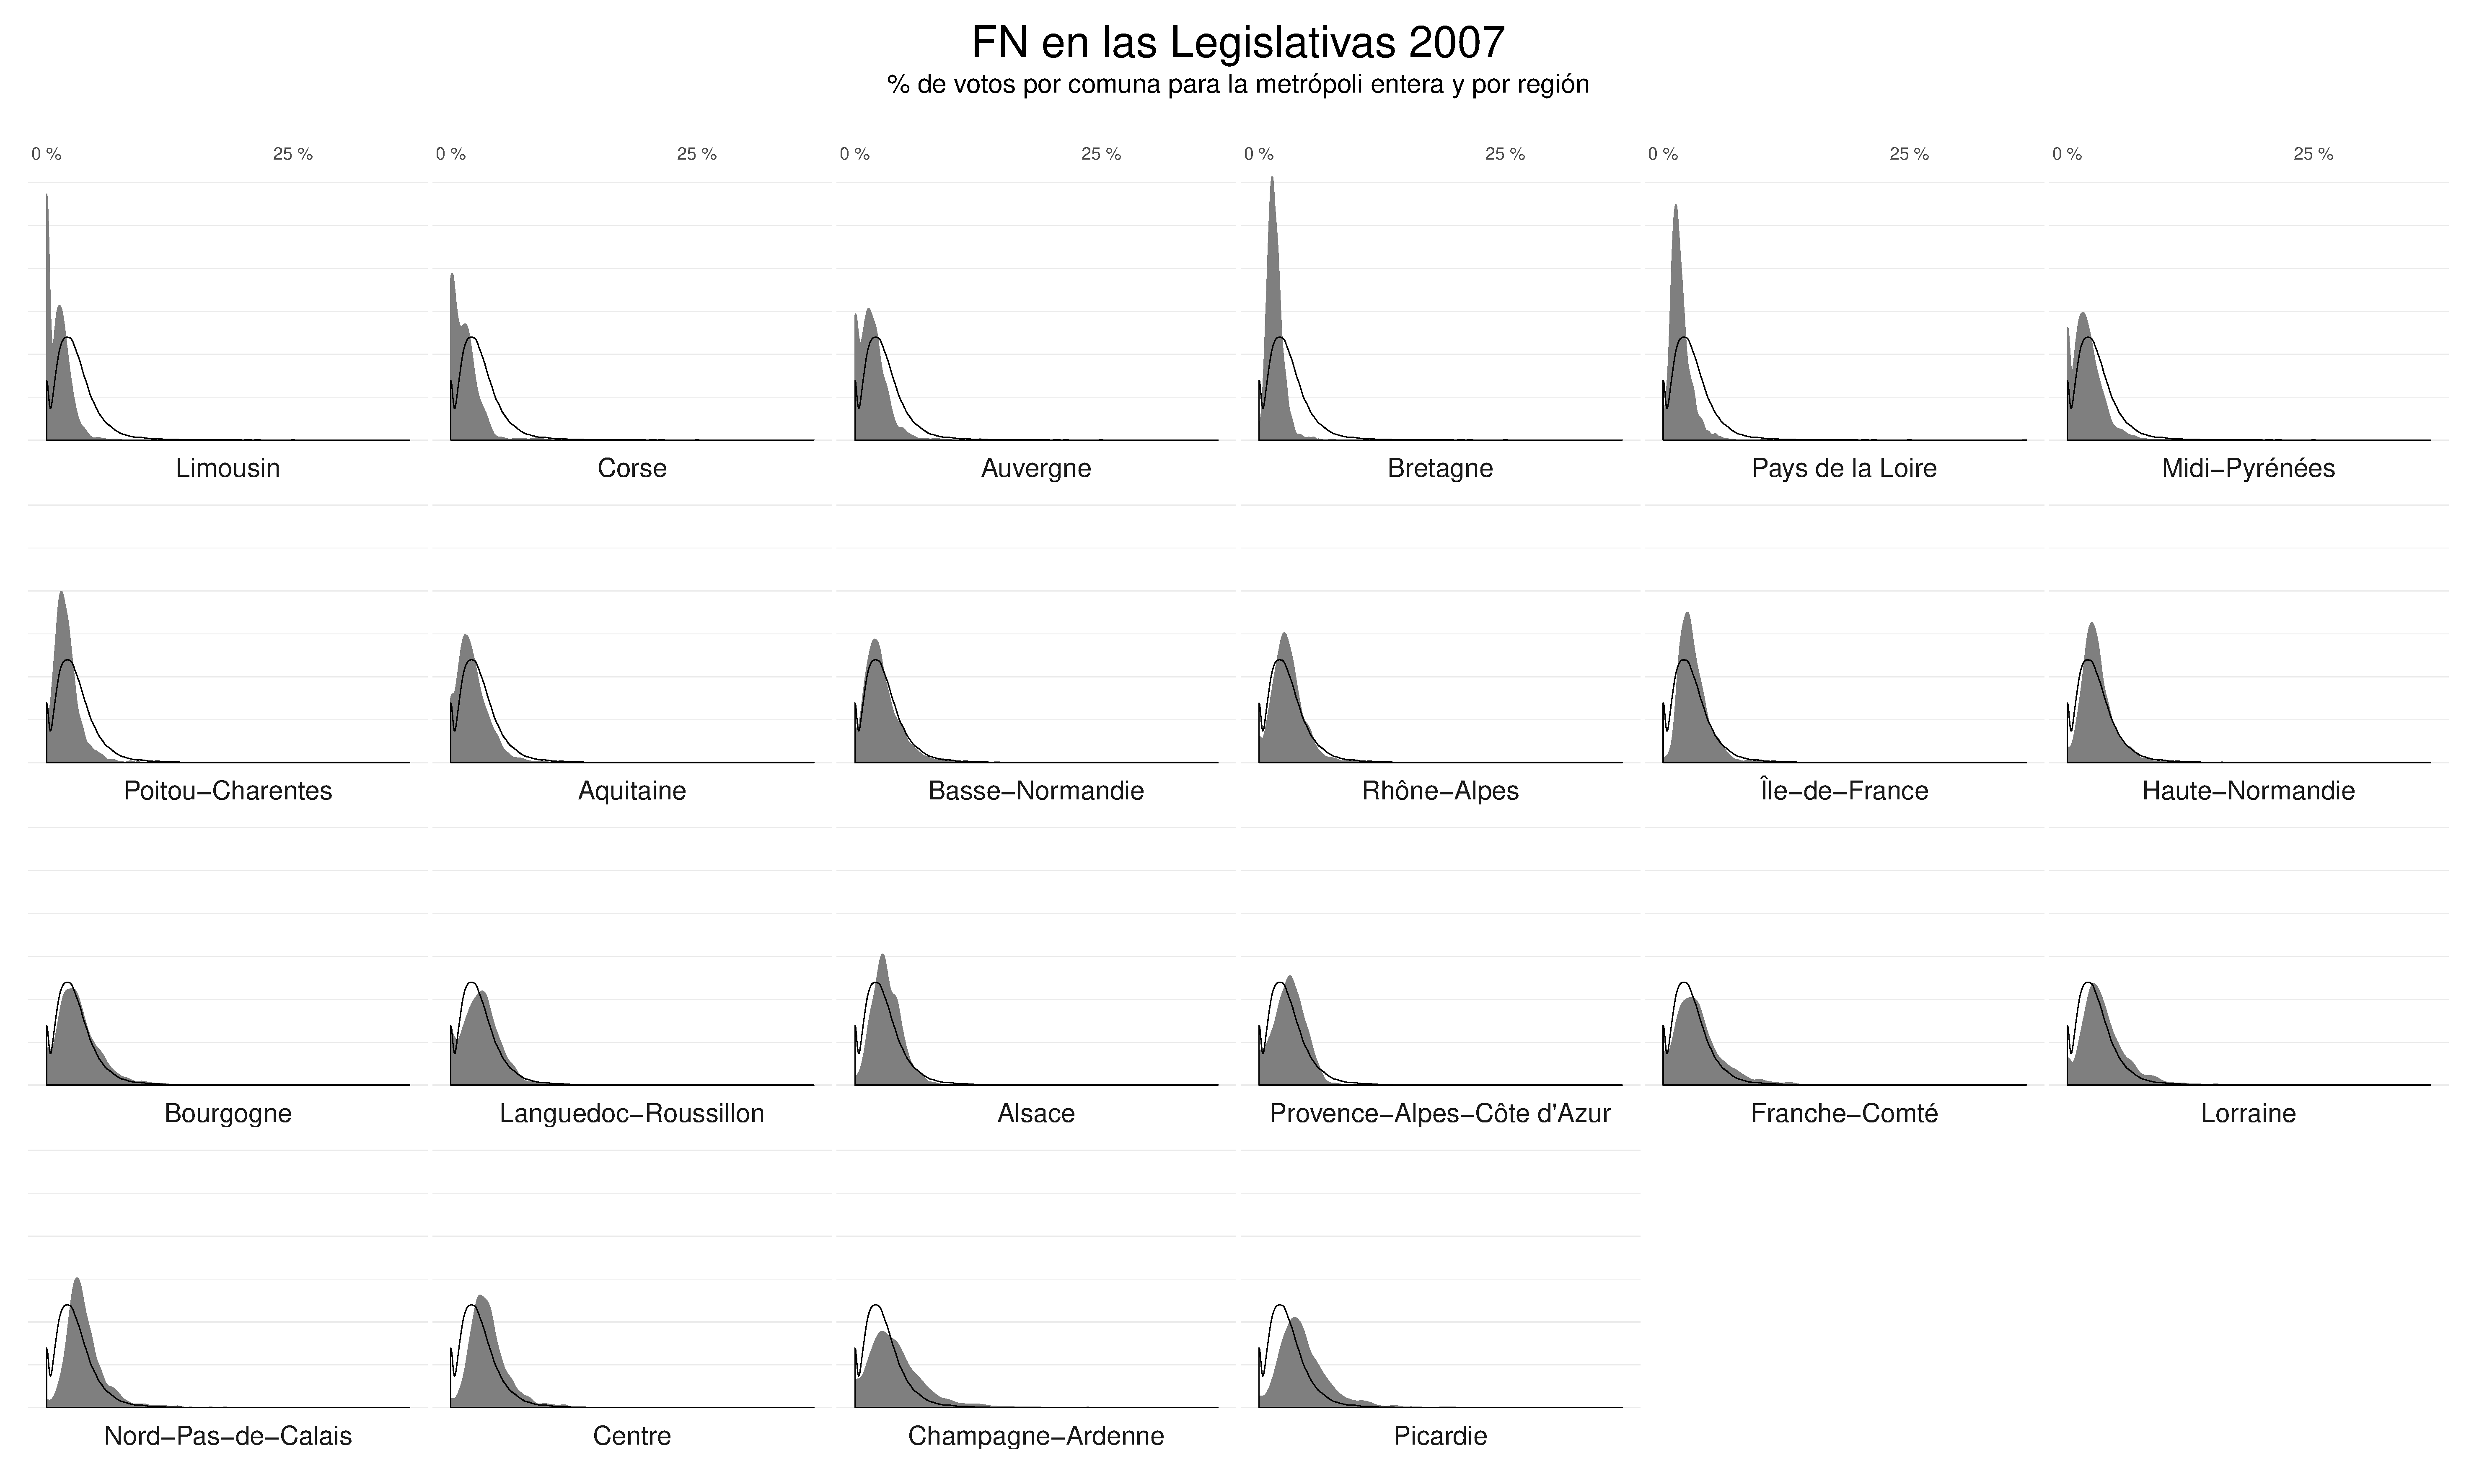
\includegraphics[scale=0.1]{Pct_Votos_Por_Comuna_FN_Reg_L07}
	\caption{Distribuciones regionales del porcentaje de votos recibidos por las candidaturas frontistas en las elecciones legislativas del 2007; las distribuciones rellenas de color son las distribuciones considerando solo las comunas de la región respectiva mientras que la distribución sin relleno es la distribución considerando todas las comunas de la metrópoli. Fuente: elaboración propia con base en los datos electorales oficiales del Ministerio del Interior francés.}
	\label{fig:Ej_Votos_Por_Reg_L07}	
\end{figure}

\begin{figure}[h]
	\centering
	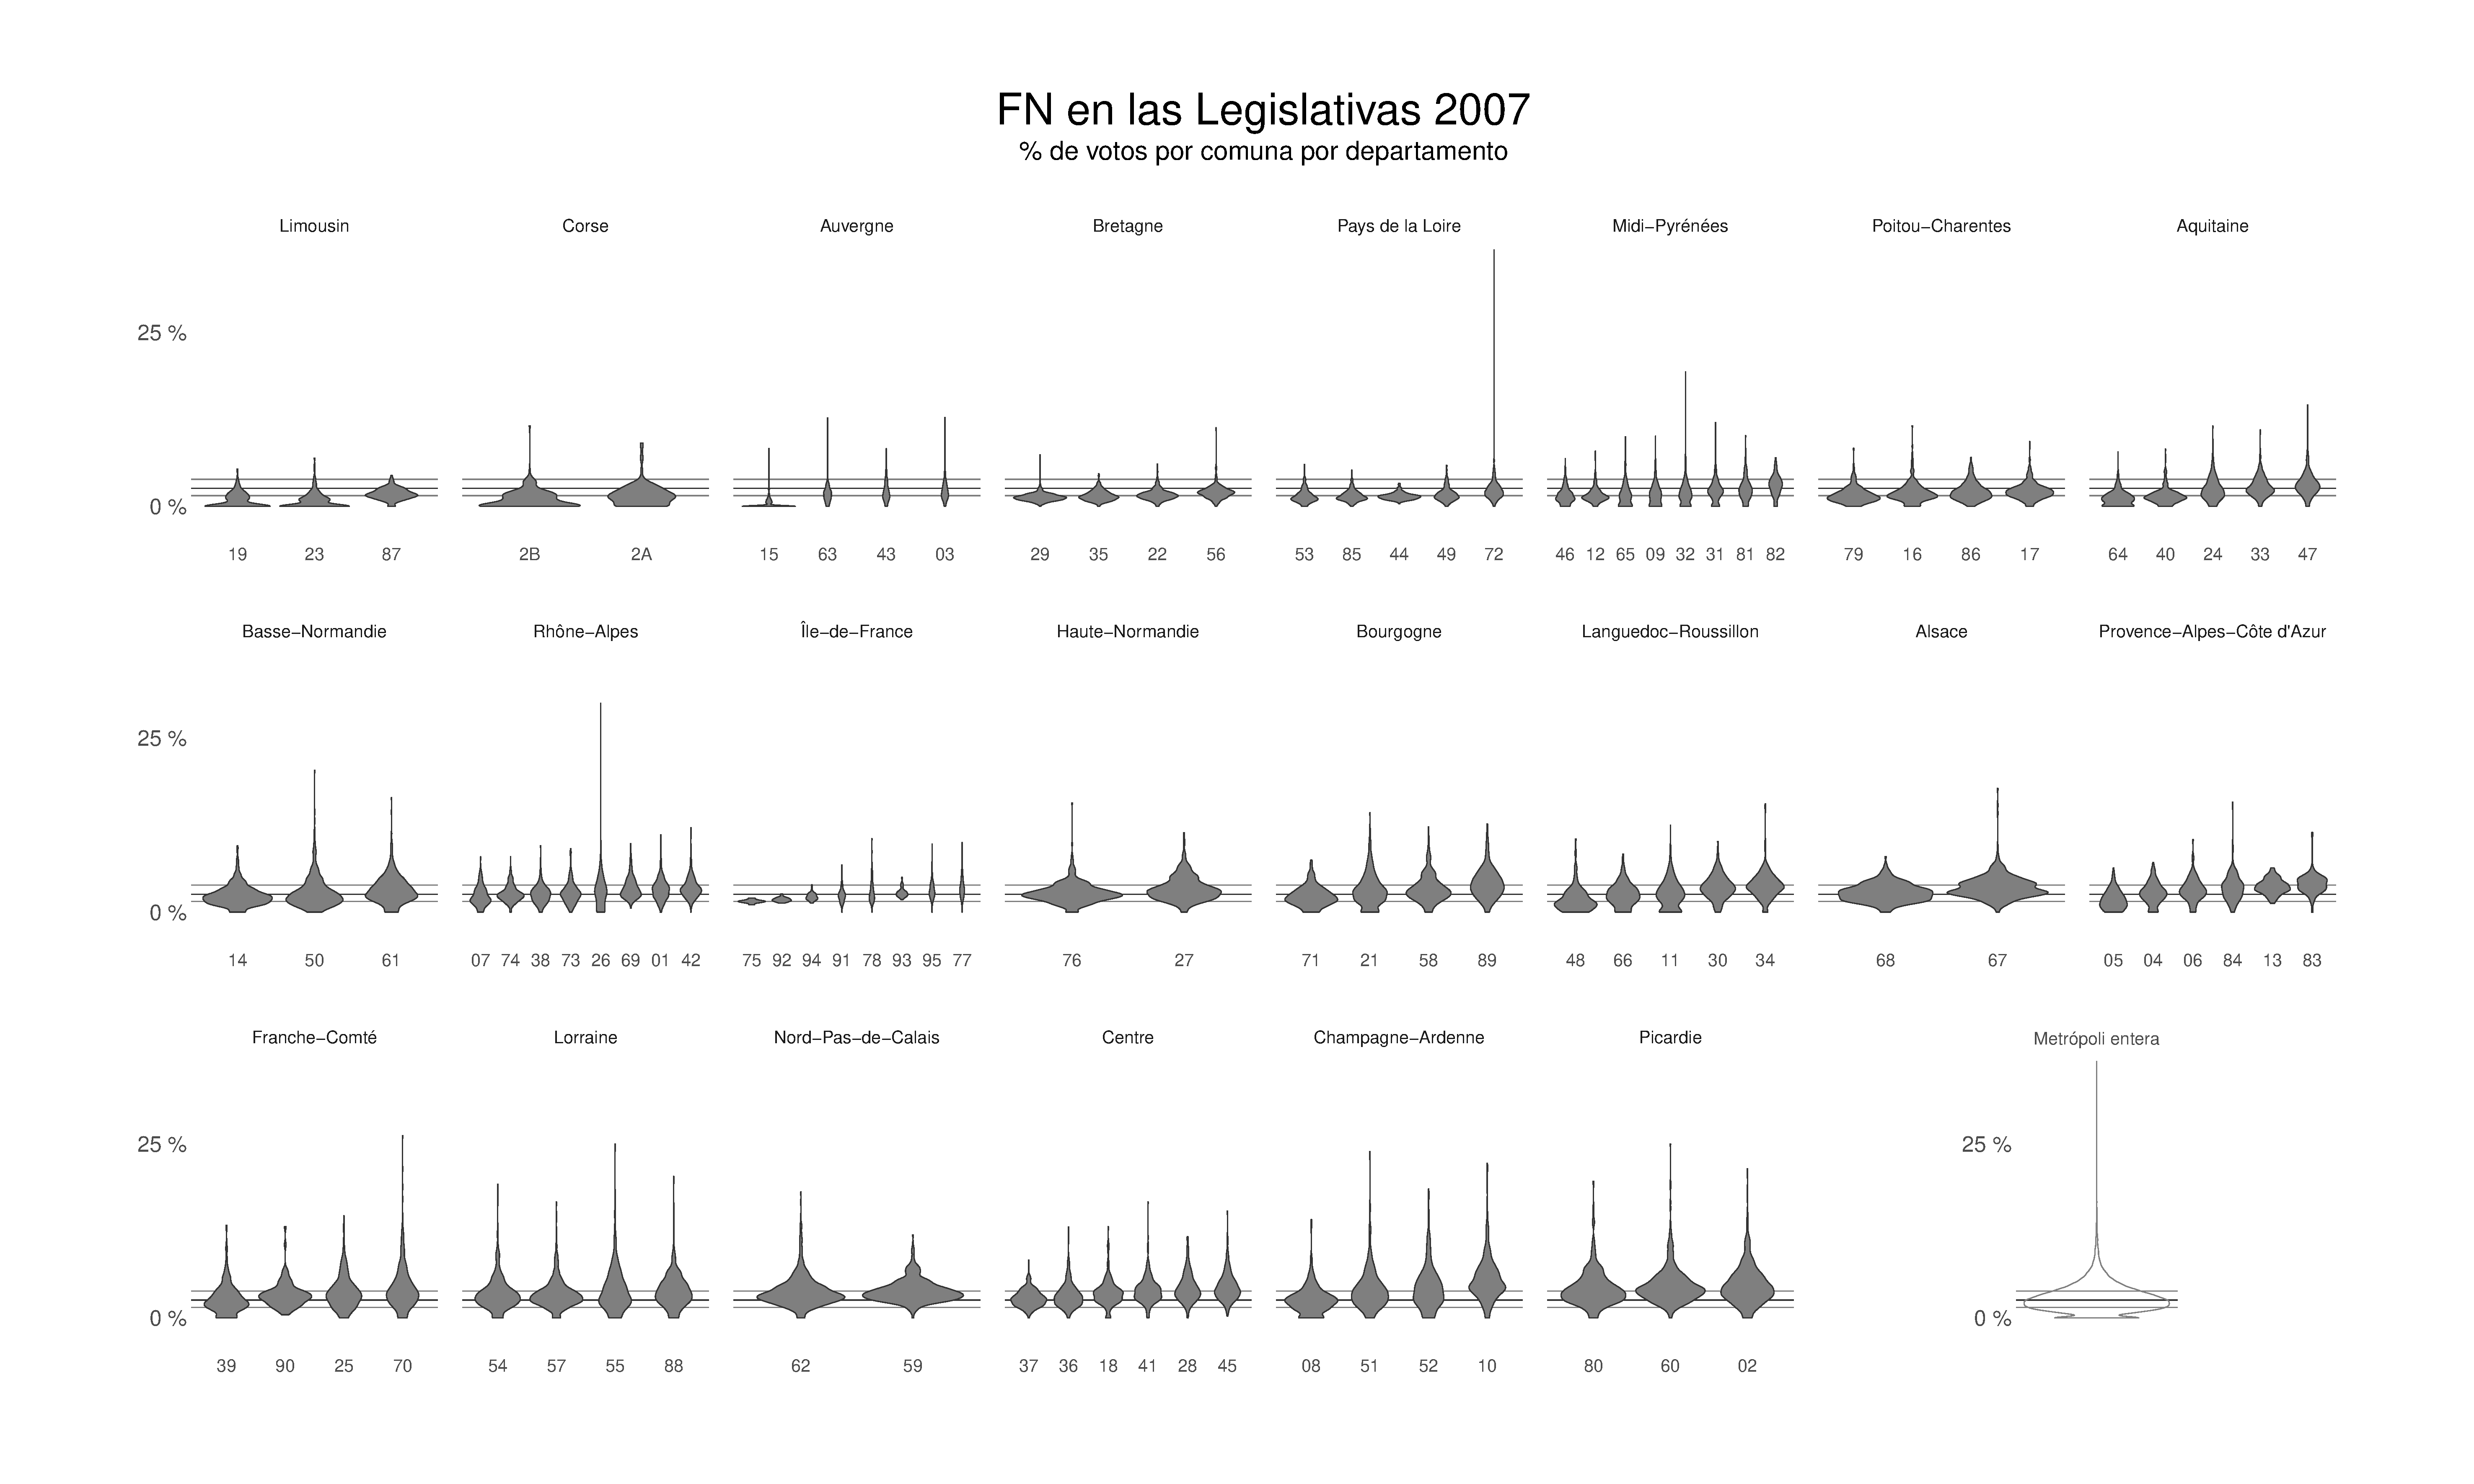
\includegraphics[scale=0.12]{Pct_Votos_Por_Comuna_FN_Dpto_L07}
	\caption{Distribuciones departamentales del porcentaje de votos recibidos por las candidaturas frontistas en las elecciones legislativas del 2007; los violines rellenos de color son las distribuciones considerando solo las comunas del departamento correspondiente mientras que las 3 líneas horizontales representan una referencia al rango intercuartílico y la mediana de la distribución considerando todas las comunas de la metrópoli, misma que puede verse en el panel inferior derecho. Fuente: elaboración propia con base en los datos electorales oficiales del Ministerio del Interior francés.}
	\label{fig:Ej_Votos_Por_Dpto_L07}	
\end{figure}

\begin{figure}[h]
	\centering
	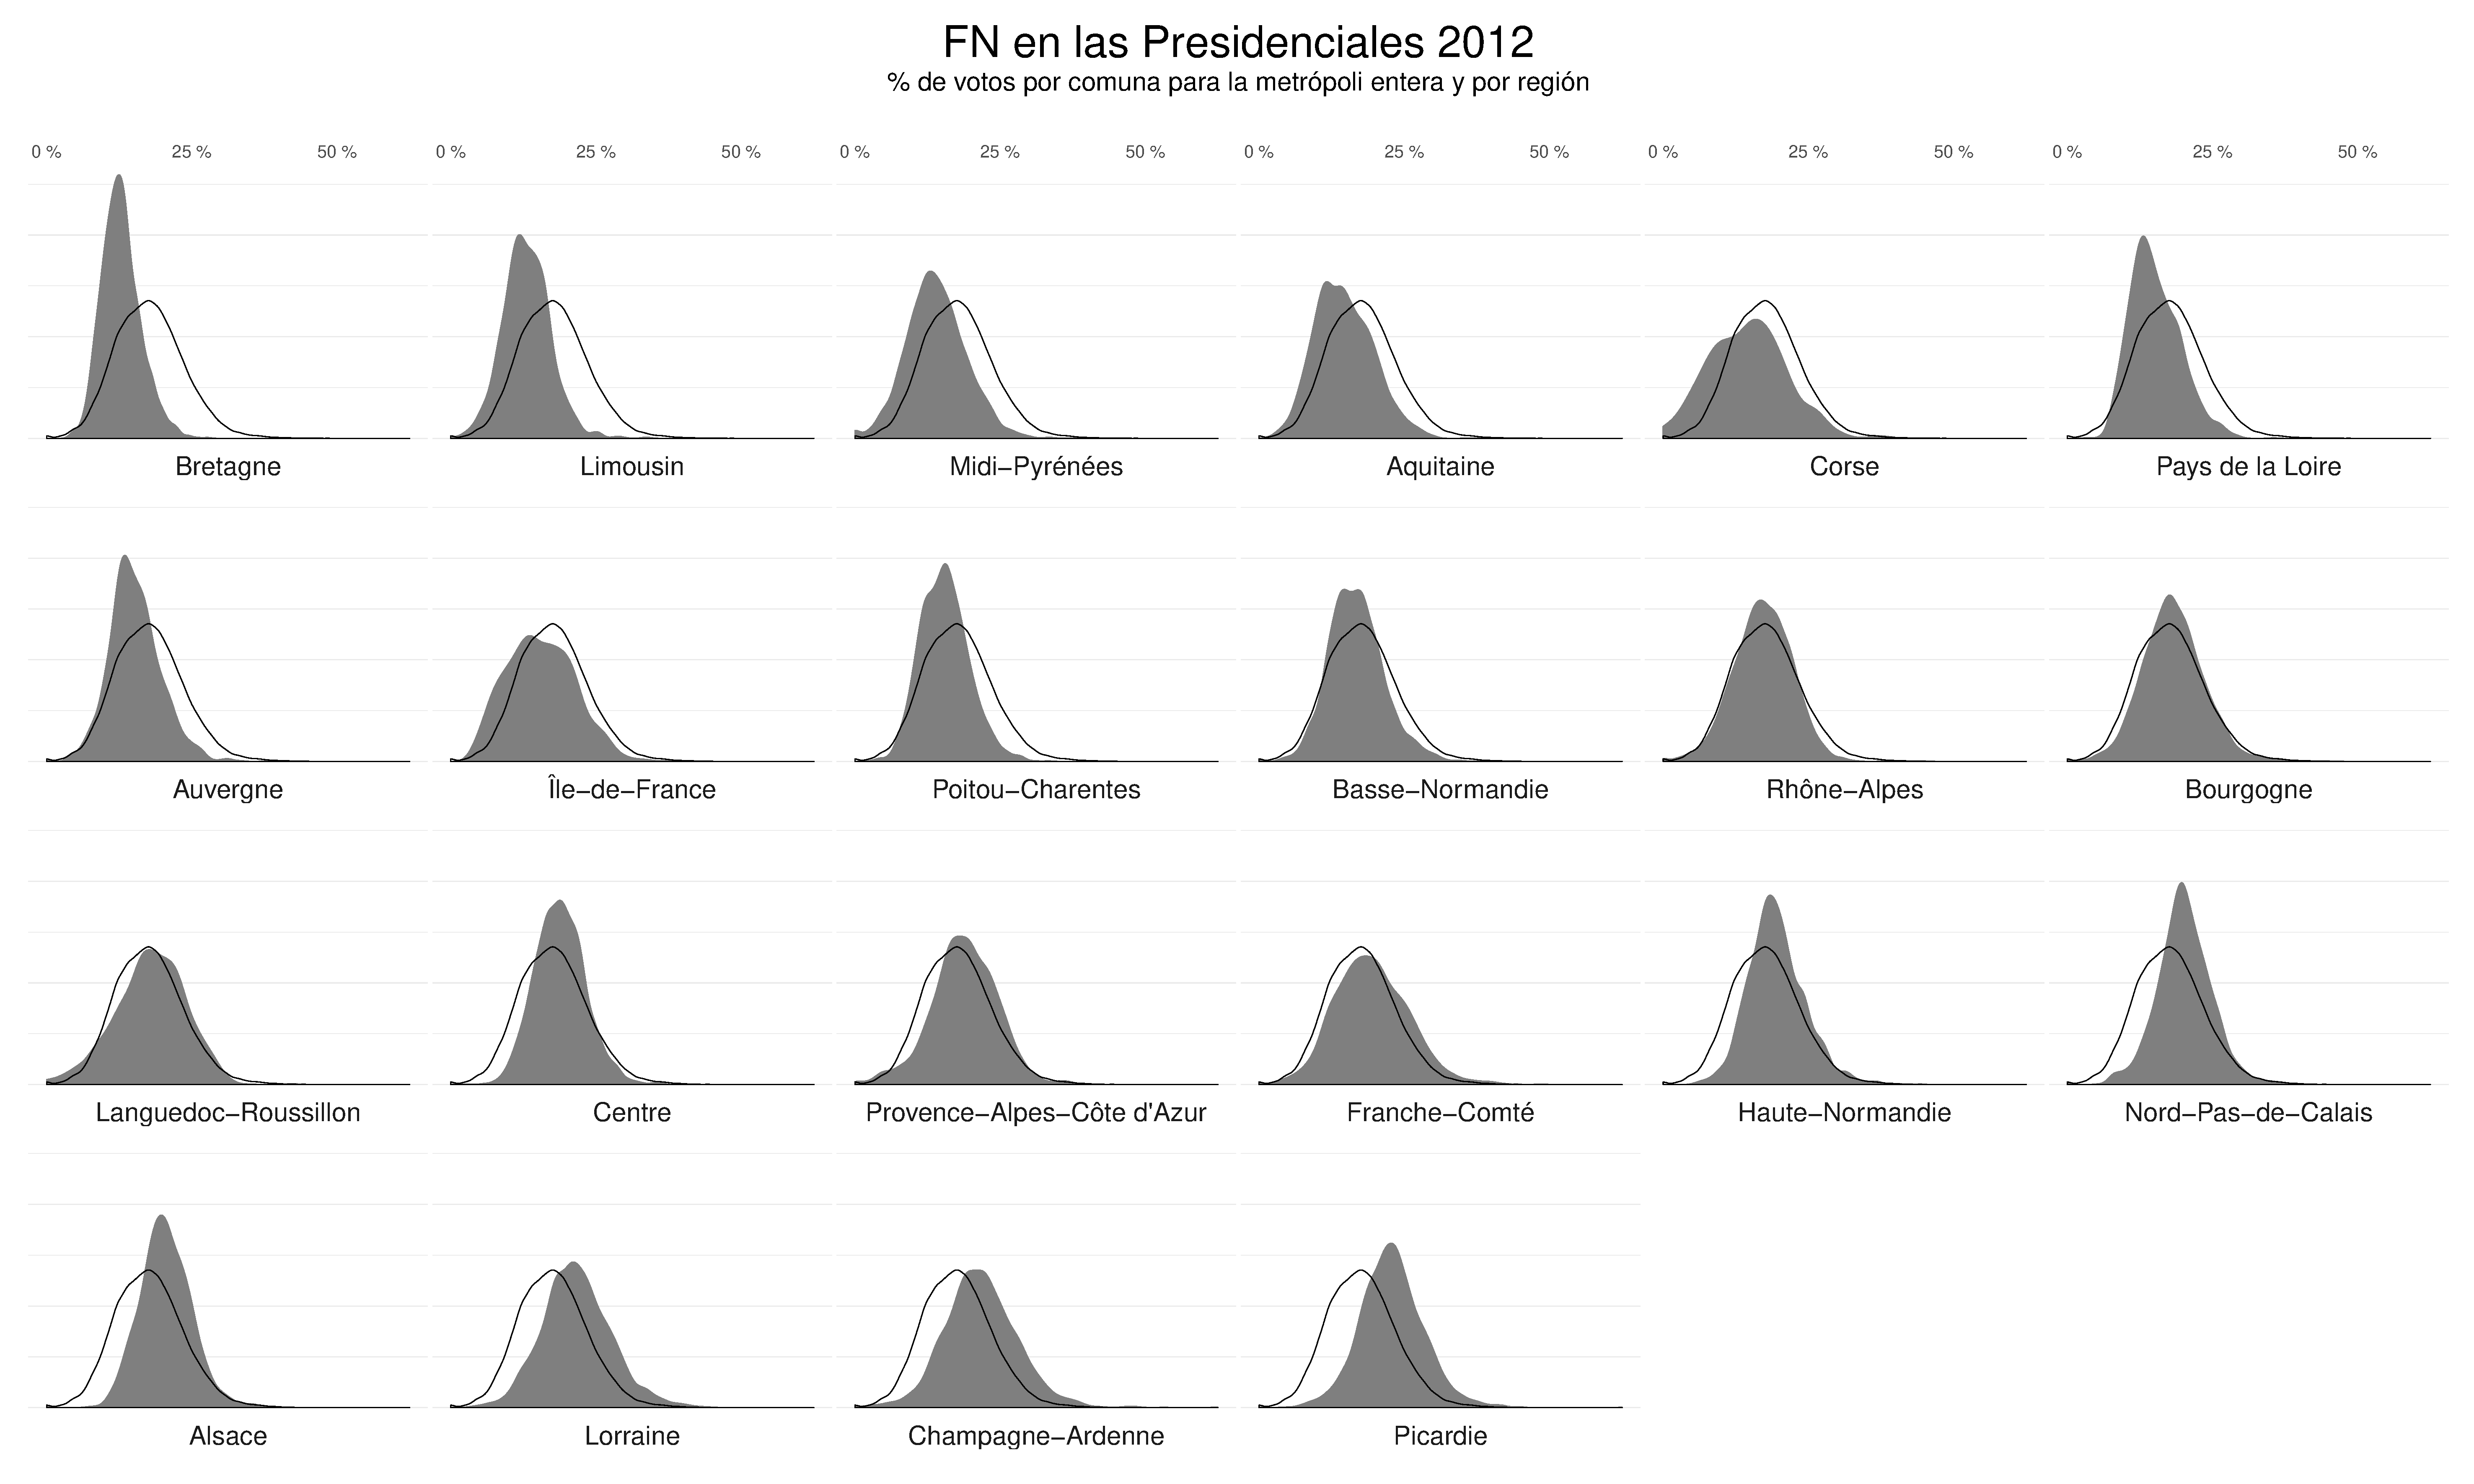
\includegraphics[scale=0.1]{Pct_Votos_Por_Comuna_FN_Reg_P12}
	\caption{Distribuciones regionales del porcentaje de votos recibidos por Marine Le Pen en las elecciones presidenciales del 2012; las distribuciones rellenas de color son las distribuciones considerando solo las comunas de la región respectiva mientras que la distribución sin relleno es la distribución considerando todas las comunas de la metrópoli. Fuente: elaboración propia con base en los datos electorales oficiales del Ministerio del Interior francés.}
	\label{fig:Ej_Votos_Por_Reg_P12}	
\end{figure}

\begin{figure}[h]
	\centering
	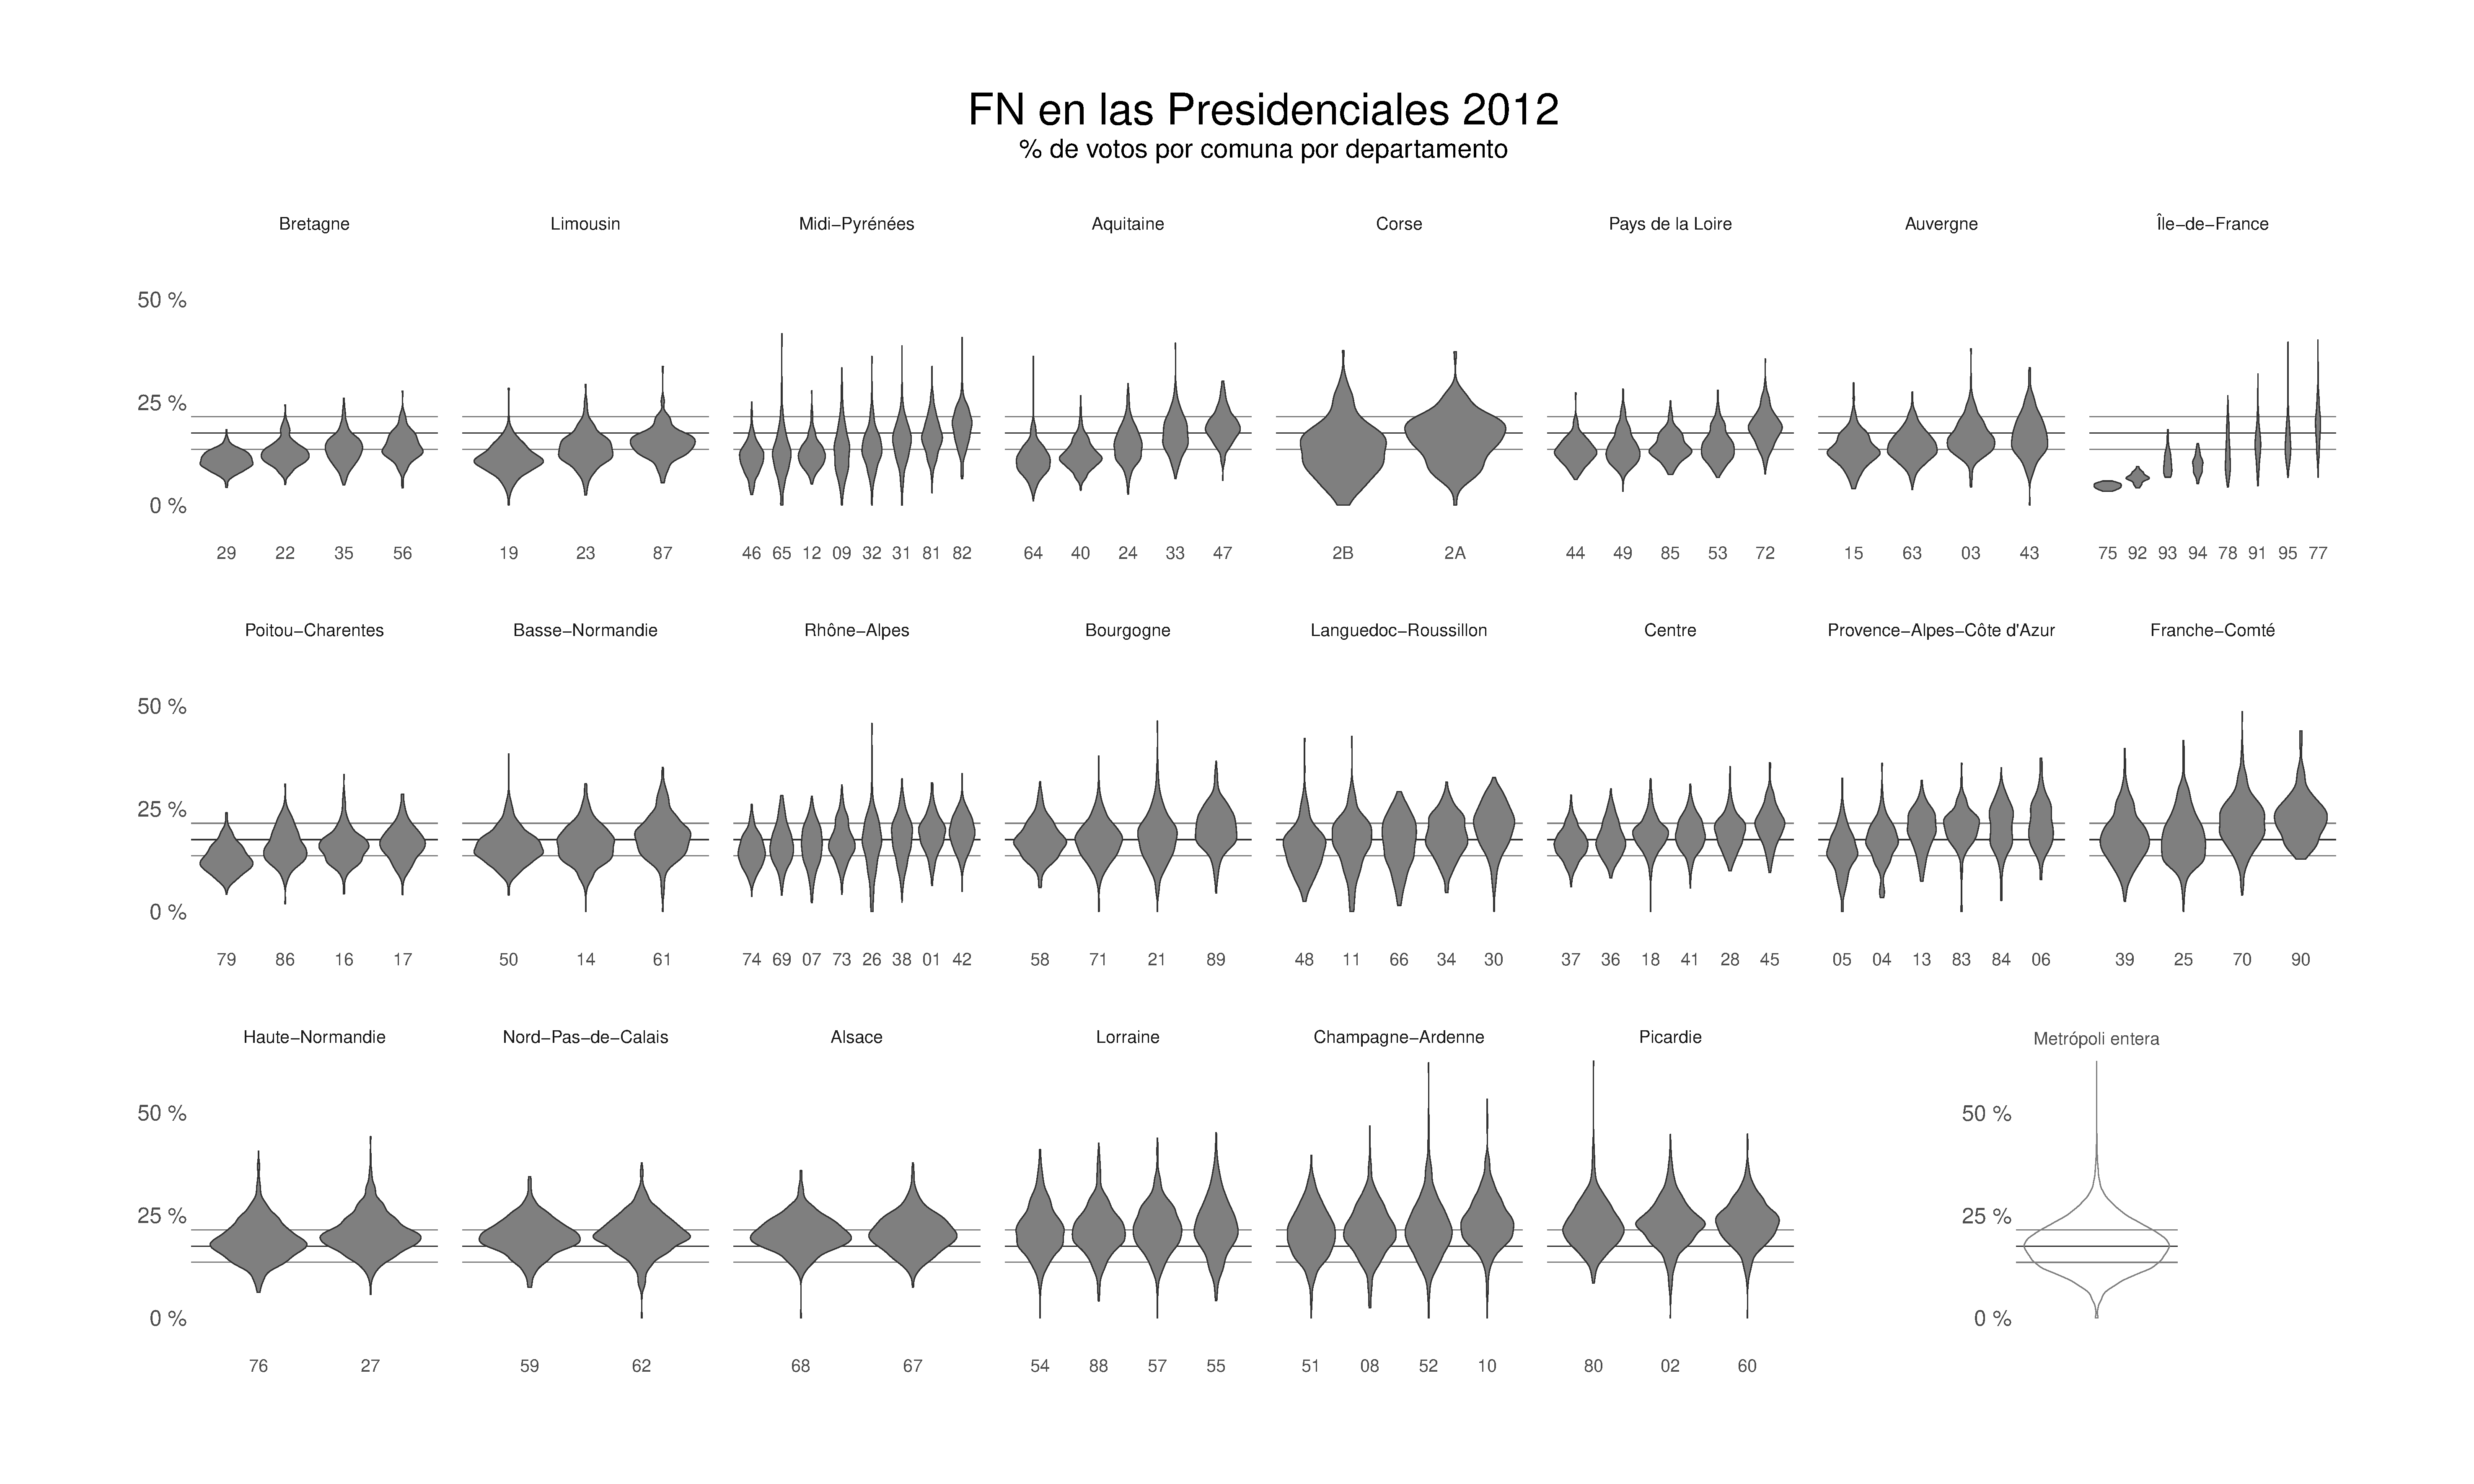
\includegraphics[scale=0.12]{Pct_Votos_Por_Comuna_FN_Dpto_P12}
	\caption{Distribuciones departamentales del porcentaje de votos recibidos por Marine Le Pen en las elecciones presidenciales de 2012; los violines rellenos de color son las distribuciones considerando solo las comunas del departamento correspondiente mientras que las 3 líneas horizontales representan una referencia al rango intercuartílico y la mediana de la distribución considerando todas las comunas de la metrópoli, misma que puede verse en el panel inferior derecho. Fuente: elaboración propia con base en los datos electorales oficiales del Ministerio del Interior francés.}
	\label{fig:Ej_Votos_Por_Dpto_P12}	
\end{figure}

\begin{figure}[h]
	\centering
	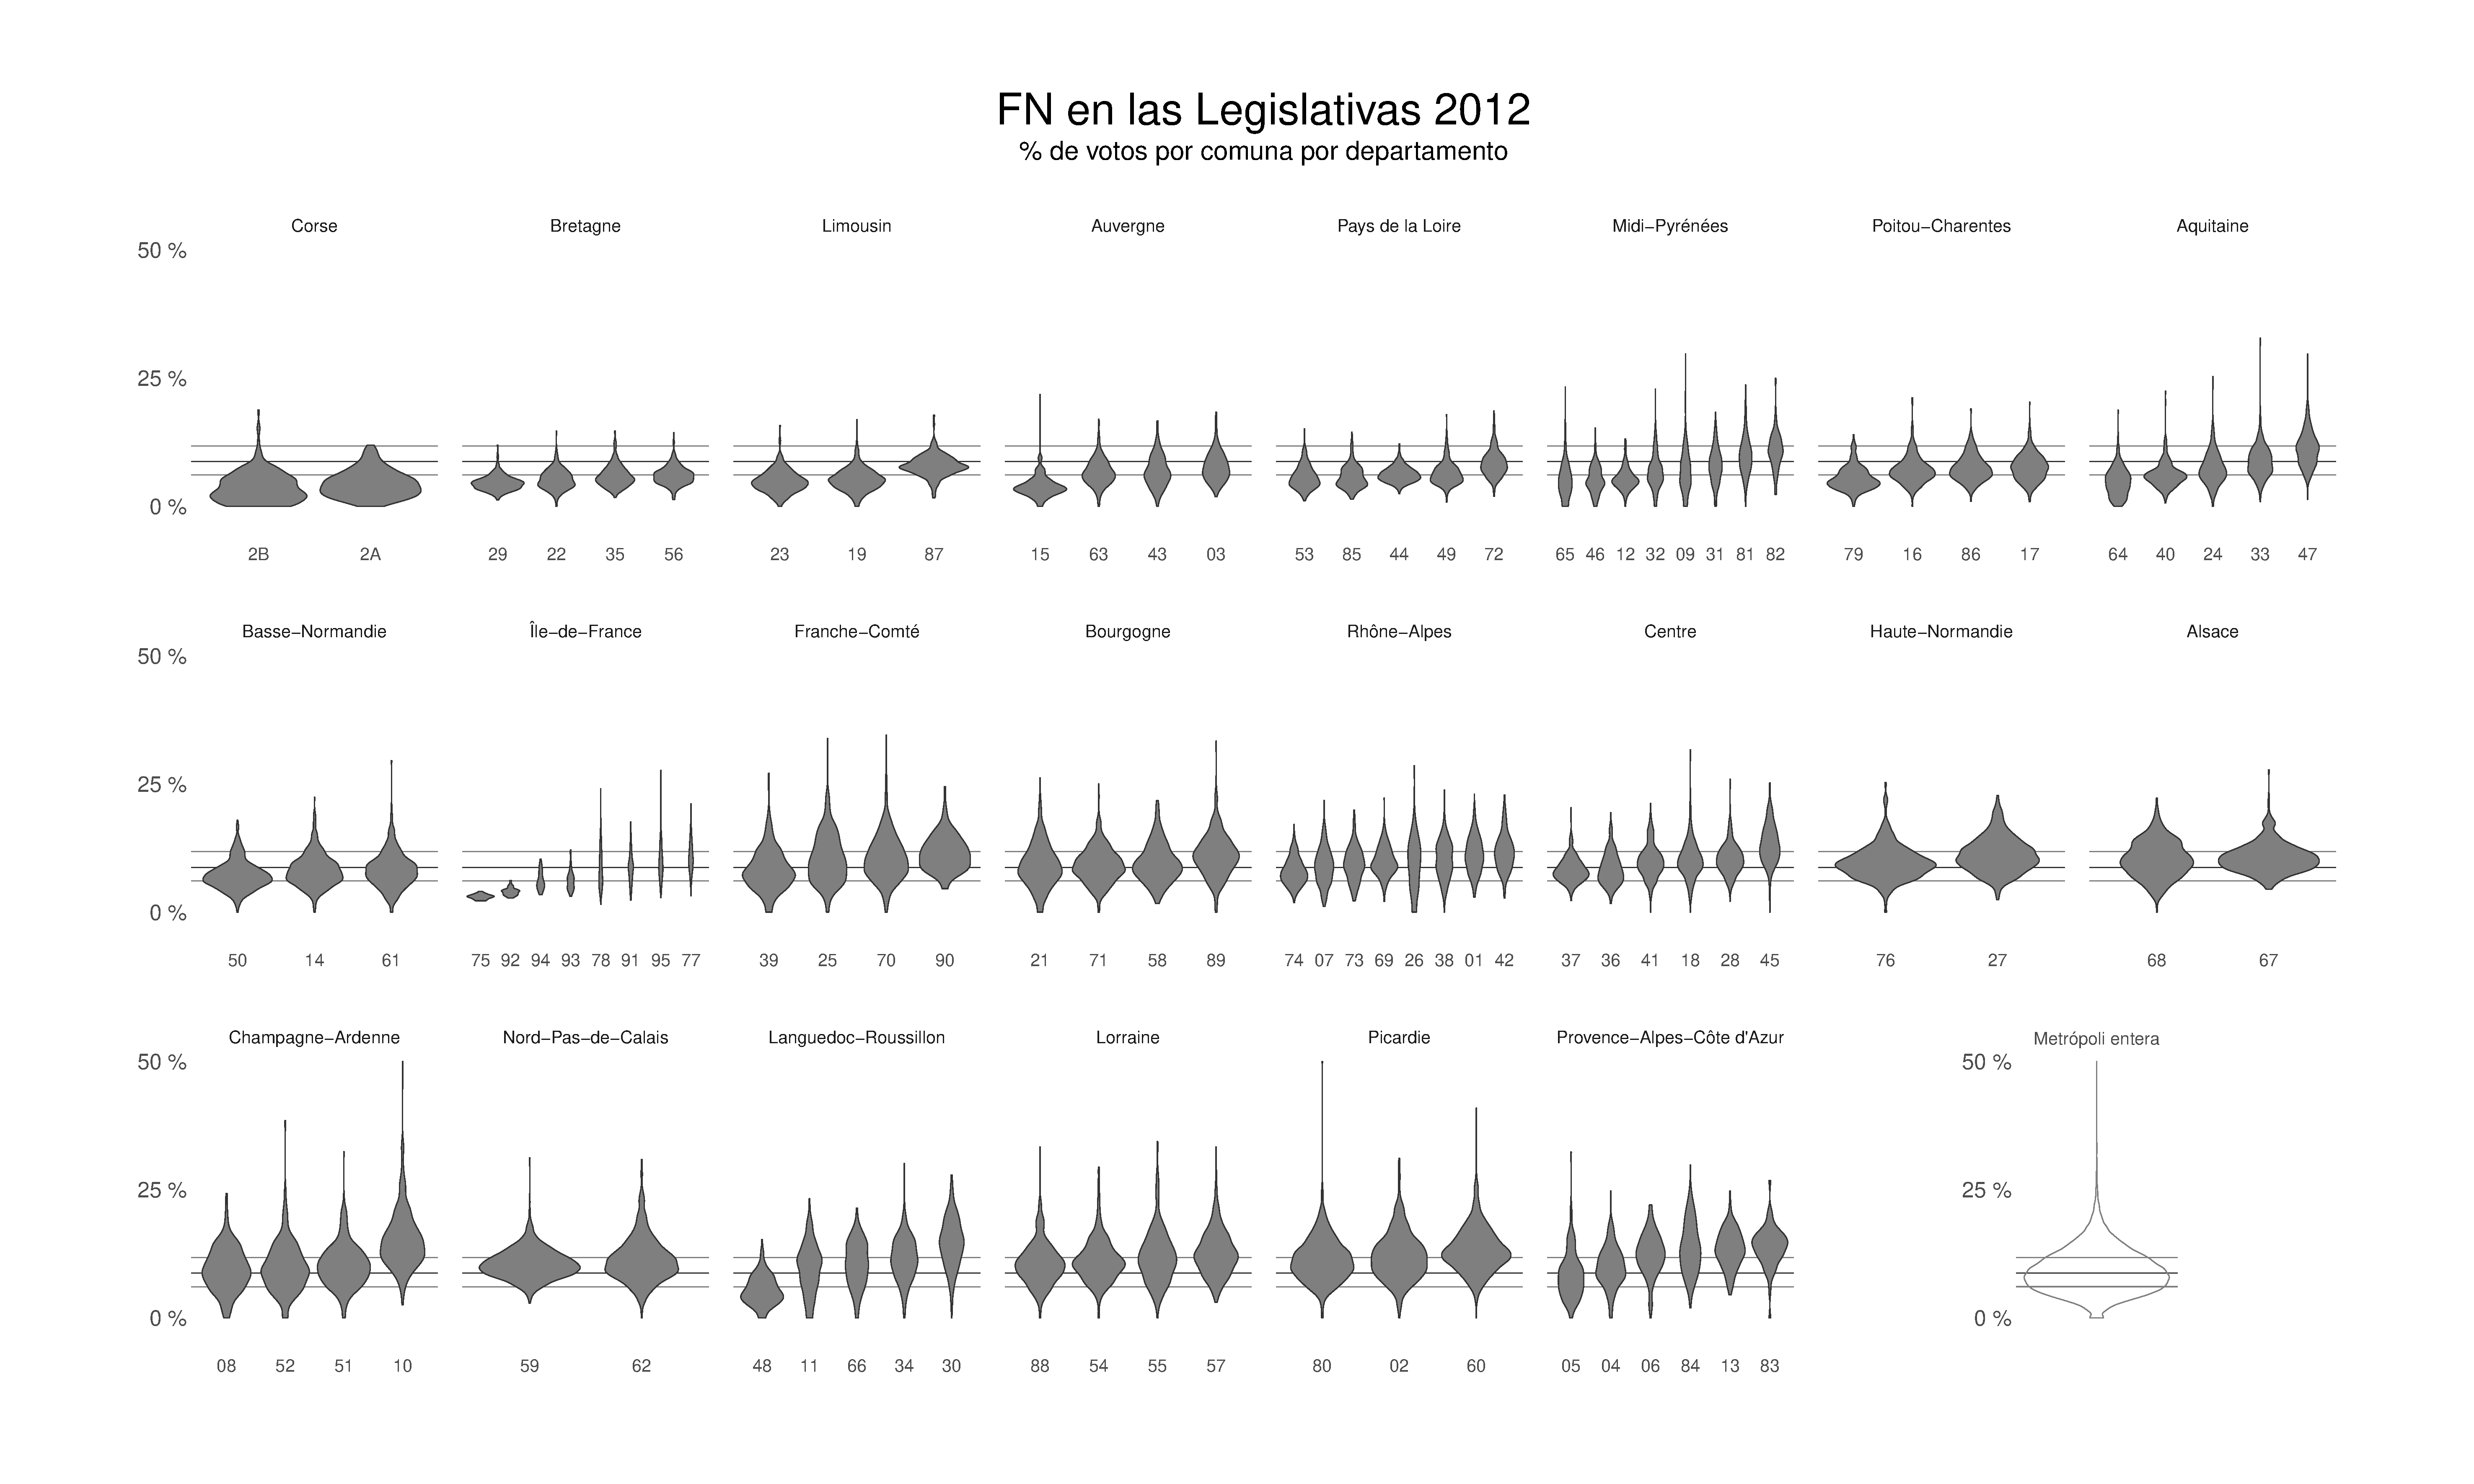
\includegraphics[scale=0.12]{Pct_Votos_Por_Comuna_FN_Dpto_L12}
	\caption{Distribuciones departamentales del porcentaje de votos recibidos por las candidaturas frontistas en las elecciones legislativas del 2012; los violines rellenos de color son las distribuciones considerando solo las comunas del departamento correspondiente mientras que las 3 líneas horizontales representan una referencia al rango intercuartílico y la mediana de la distribución considerando todas las comunas de la metrópoli, misma que puede verse en el panel inferior derecho. Fuente: elaboración propia con base en los datos electorales oficiales del Ministerio del Interior francés.}
	\label{fig:Ej_Votos_Por_Dpto_L12}	
\end{figure}
%\chapter{Familia exponencial}

En este anexo presento 3 distribuciones que pertenecen a la familia exponencial. Para ello, presento de nueva cuenta definición de la familia exponencial: 

\textbf{Definición \ref{def:Fam_Exp}. Familia Exponencial}\\
Sea $Y$ una variable aleatoria con función de distribución $p\left(Y|\theta = (\theta_1,\dots,\theta_k)\right)$ tal que 
\begin{equation*}
p\left(Y|\theta = (\theta_1,\dots,\theta_k)\right) = a(\theta)b(Y)exp\left\lbrace\sum\limits_{j=1}^k c_j(\theta)d_j(Y)\right\rbrace,
\end{equation*}
donde $a, b$ y todas las $c_j$ y $d_j$ son funciones conocidas. Se dice entonces que $Y$ pertenece a la \textbf{familia exponencial}.
 

\begin{enumerate}

\item \textbf{Distribución Normal}

\begin{align*}
Y &\sim N(\mu,\sigma^2) \\
p(y|\theta = (\mu,\sigma^2)) &=\dfrac{1}{\sqrt{2\pi\sigma^2}}exp\left\lbrace-\dfrac{1}{2\sigma^2}(y-\mu)^2\right\rbrace\\
& = \dfrac{1}{\sqrt{2\pi\sigma^2}}exp\left\lbrace-\dfrac{y^2-2y\mu+\mu^2}{2\sigma^2}\right\rbrace\\
& = \dfrac{1}{\sqrt{2\pi\sigma^2}}exp\left\lbrace-\dfrac{\mu^2}{2\sigma^2}\right\rbrace exp\left\lbrace y\dfrac{\mu}{\sigma^2} - y^2\dfrac{1}{\sigma^2}\right\rbrace \\
\intertext{De aquí podemos ver entonces que:}
a(\theta = (\mu,\sigma^2)) &= \dfrac{1}{\sqrt{2\pi\sigma^2}}exp\left\lbrace-\dfrac{\mu^2}{2\sigma^2}\right\rbrace & b(y) &= 1 \\
c_1(\theta = (\mu,\sigma^2)) &= \dfrac{\mu}{\sigma^2} & d_1(y) &= y\\ 
c_2(\theta = (\mu,\sigma^2)) &= -\dfrac{1}{\sigma^2} & d_2(y) &= y^2\\ 
\end{align*}

\item \textbf{Distribución Poisson}
\begin{align*}
Y &\sim Poi(\lambda) \\
p(y|\theta = \lambda) &=\dfrac{\lambda^ye^{-\lambda}}{y!}I_{\mathbb{N}}(y) \\
& = e^{-\lambda}\dfrac{I_{\mathbb{N}}(y)}{y!}exp\left\lbrace y\, ln(\lambda)\right\rbrace 
\intertext{De aquí podemos ver entonces que:}
a(\theta = \lambda) &= e^{-\lambda} & b(y) &= \dfrac{I_{\mathbb{N}}(y)}{y!} \\
c_1(\theta = \lambda) &= ln(\lambda) & d_1(y) &= y\\ 
\end{align*}

\item \textbf{Distribución Binomial}
Suponemos que $n$, el número de ensayos Bernoulli, es conocido. 
\begin{align*}
Y &\sim Bin(n,p) \\
p(y|\theta = p) &= {n \choose y} p^y(1-p)^{n-y}I_{\mathbb{N}_n}(y) \\
& = (1-p)^n {n \choose y} I_{\mathbb{N}_n}(y)\left(\dfrac{p}{1-p}\right)^y \\
& = (1-p)^n {n \choose y} I_{\mathbb{N}_n}(y) exp\left\lbrace y\,ln\left(\dfrac{p}{1-p}\right)\right\rbrace
\intertext{De aquí podemos ver entonces que:}
a(\theta = p) &= (1-p)^n & b(y) &= {n \choose y} I_{\mathbb{N}_n}(y) \\
c_1(\theta = p) &= ln\left(\dfrac{p}{1-p}\right) & d_1(y) &= y\\ 
\end{align*}

\end{enumerate}


%%%%%%%%%%%%%%%%%%%%%%%%%%%%%%%%%%%%%%%%%%%%%%%%%%%%%%%%%%%%%
%%  REFERENCIAS %%%
%%%%%%%%%%%%%%%%%%%%%%%%%%%%%%%%%%%%%%%%%%%%%%%%%%%%%%%%%%%%%

\addcontentsline{toc}{part}{Referencias}
\part*{Referencias}
\printbibliography[title = {Referencias}]

%%%%%%%%%%%%%%%%%%%%%%%%%%%%%%%%%%%%%%%%%%%%%%%%%%%%%%%%%%%%%
%%  FINAL DEL DOCUMENTO %%%
%%%%%%%%%%%%%%%%%%%%%%%%%%%%%%%%%%%%%%%%%%%%%%%%%%%%%%%%%%%%%

\end{document}